\documentclass[12pt,]{krantz}
\usepackage{lmodern}
\usepackage{amssymb,amsmath}
\usepackage{ifxetex,ifluatex}
\usepackage{fixltx2e} % provides \textsubscript
\ifnum 0\ifxetex 1\fi\ifluatex 1\fi=0 % if pdftex
  \usepackage[T1]{fontenc}
  \usepackage[utf8]{inputenc}
\else % if luatex or xelatex
  \ifxetex
    \usepackage{mathspec}
  \else
    \usepackage{fontspec}
  \fi
  \defaultfontfeatures{Ligatures=TeX,Scale=MatchLowercase}
    \setmonofont[Mapping=tex-ansi,Scale=0.7]{Source Code Pro}
\fi
% use upquote if available, for straight quotes in verbatim environments
\IfFileExists{upquote.sty}{\usepackage{upquote}}{}
% use microtype if available
\IfFileExists{microtype.sty}{%
\usepackage{microtype}
\UseMicrotypeSet[protrusion]{basicmath} % disable protrusion for tt fonts
}{}
\usepackage[margin=1in]{geometry}
\usepackage{hyperref}
\PassOptionsToPackage{usenames,dvipsnames}{color} % color is loaded by hyperref
\hypersetup{unicode=true,
            pdftitle={Predictive Models: Explore, Explain, and Debug},
            pdfauthor={Przemyslaw Biecek and Tomasz Burzykowski},
            colorlinks=true,
            linkcolor=Maroon,
            citecolor=Blue,
            urlcolor=Blue,
            breaklinks=true}
\urlstyle{same}  % don't use monospace font for urls
\usepackage{natbib}
\bibliographystyle{apalike}
\usepackage{color}
\usepackage{fancyvrb}
\newcommand{\VerbBar}{|}
\newcommand{\VERB}{\Verb[commandchars=\\\{\}]}
\DefineVerbatimEnvironment{Highlighting}{Verbatim}{commandchars=\\\{\}}
% Add ',fontsize=\small' for more characters per line
\usepackage{framed}
\definecolor{shadecolor}{RGB}{248,248,248}
\newenvironment{Shaded}{\begin{snugshade}}{\end{snugshade}}
\newcommand{\AlertTok}[1]{\textcolor[rgb]{0.94,0.16,0.16}{#1}}
\newcommand{\AnnotationTok}[1]{\textcolor[rgb]{0.56,0.35,0.01}{\textbf{\textit{#1}}}}
\newcommand{\AttributeTok}[1]{\textcolor[rgb]{0.77,0.63,0.00}{#1}}
\newcommand{\BaseNTok}[1]{\textcolor[rgb]{0.00,0.00,0.81}{#1}}
\newcommand{\BuiltInTok}[1]{#1}
\newcommand{\CharTok}[1]{\textcolor[rgb]{0.31,0.60,0.02}{#1}}
\newcommand{\CommentTok}[1]{\textcolor[rgb]{0.56,0.35,0.01}{\textit{#1}}}
\newcommand{\CommentVarTok}[1]{\textcolor[rgb]{0.56,0.35,0.01}{\textbf{\textit{#1}}}}
\newcommand{\ConstantTok}[1]{\textcolor[rgb]{0.00,0.00,0.00}{#1}}
\newcommand{\ControlFlowTok}[1]{\textcolor[rgb]{0.13,0.29,0.53}{\textbf{#1}}}
\newcommand{\DataTypeTok}[1]{\textcolor[rgb]{0.13,0.29,0.53}{#1}}
\newcommand{\DecValTok}[1]{\textcolor[rgb]{0.00,0.00,0.81}{#1}}
\newcommand{\DocumentationTok}[1]{\textcolor[rgb]{0.56,0.35,0.01}{\textbf{\textit{#1}}}}
\newcommand{\ErrorTok}[1]{\textcolor[rgb]{0.64,0.00,0.00}{\textbf{#1}}}
\newcommand{\ExtensionTok}[1]{#1}
\newcommand{\FloatTok}[1]{\textcolor[rgb]{0.00,0.00,0.81}{#1}}
\newcommand{\FunctionTok}[1]{\textcolor[rgb]{0.00,0.00,0.00}{#1}}
\newcommand{\ImportTok}[1]{#1}
\newcommand{\InformationTok}[1]{\textcolor[rgb]{0.56,0.35,0.01}{\textbf{\textit{#1}}}}
\newcommand{\KeywordTok}[1]{\textcolor[rgb]{0.13,0.29,0.53}{\textbf{#1}}}
\newcommand{\NormalTok}[1]{#1}
\newcommand{\OperatorTok}[1]{\textcolor[rgb]{0.81,0.36,0.00}{\textbf{#1}}}
\newcommand{\OtherTok}[1]{\textcolor[rgb]{0.56,0.35,0.01}{#1}}
\newcommand{\PreprocessorTok}[1]{\textcolor[rgb]{0.56,0.35,0.01}{\textit{#1}}}
\newcommand{\RegionMarkerTok}[1]{#1}
\newcommand{\SpecialCharTok}[1]{\textcolor[rgb]{0.00,0.00,0.00}{#1}}
\newcommand{\SpecialStringTok}[1]{\textcolor[rgb]{0.31,0.60,0.02}{#1}}
\newcommand{\StringTok}[1]{\textcolor[rgb]{0.31,0.60,0.02}{#1}}
\newcommand{\VariableTok}[1]{\textcolor[rgb]{0.00,0.00,0.00}{#1}}
\newcommand{\VerbatimStringTok}[1]{\textcolor[rgb]{0.31,0.60,0.02}{#1}}
\newcommand{\WarningTok}[1]{\textcolor[rgb]{0.56,0.35,0.01}{\textbf{\textit{#1}}}}
\usepackage{longtable,booktabs}
\usepackage{graphicx,grffile}
\makeatletter
\def\maxwidth{\ifdim\Gin@nat@width>\linewidth\linewidth\else\Gin@nat@width\fi}
\def\maxheight{\ifdim\Gin@nat@height>\textheight\textheight\else\Gin@nat@height\fi}
\makeatother
% Scale images if necessary, so that they will not overflow the page
% margins by default, and it is still possible to overwrite the defaults
% using explicit options in \includegraphics[width, height, ...]{}
\setkeys{Gin}{width=\maxwidth,height=\maxheight,keepaspectratio}
\IfFileExists{parskip.sty}{%
\usepackage{parskip}
}{% else
\setlength{\parindent}{0pt}
\setlength{\parskip}{6pt plus 2pt minus 1pt}
}
\setlength{\emergencystretch}{3em}  % prevent overfull lines
\providecommand{\tightlist}{%
  \setlength{\itemsep}{0pt}\setlength{\parskip}{0pt}}
\setcounter{secnumdepth}{5}
% Redefines (sub)paragraphs to behave more like sections
\ifx\paragraph\undefined\else
\let\oldparagraph\paragraph
\renewcommand{\paragraph}[1]{\oldparagraph{#1}\mbox{}}
\fi
\ifx\subparagraph\undefined\else
\let\oldsubparagraph\subparagraph
\renewcommand{\subparagraph}[1]{\oldsubparagraph{#1}\mbox{}}
\fi

%%% Use protect on footnotes to avoid problems with footnotes in titles
\let\rmarkdownfootnote\footnote%
\def\footnote{\protect\rmarkdownfootnote}

%%% Change title format to be more compact
\usepackage{titling}

% Create subtitle command for use in maketitle
\providecommand{\subtitle}[1]{
  \posttitle{
    \begin{center}\large#1\end{center}
    }
}

\setlength{\droptitle}{-2em}

  \title{Predictive Models: Explore, Explain, and Debug}
    \pretitle{\vspace{\droptitle}\centering\huge}
  \posttitle{\par}
  \subtitle{Human-Centered Interpretable Machine Learning}
  \author{Przemyslaw Biecek and Tomasz Burzykowski}
    \preauthor{\centering\large\emph}
  \postauthor{\par}
      \predate{\centering\large\emph}
  \postdate{\par}
    \date{2019-07-17}

\usepackage{booktabs}

\usepackage{amsthm}
\newtheorem{theorem}{Theorem}[section]
\newtheorem{lemma}{Lemma}[section]
\theoremstyle{definition}
\newtheorem{definition}{Definition}[section]
\newtheorem{corollary}{Corollary}[section]
\newtheorem{proposition}{Proposition}[section]
\theoremstyle{definition}
\newtheorem{example}{Example}[section]
\theoremstyle{definition}
\newtheorem{exercise}{Exercise}[section]
\theoremstyle{remark}
\newtheorem*{remark}{Remark}
\newtheorem*{solution}{Solution}
\begin{document}
\maketitle

{
\hypersetup{linkcolor=black}
\setcounter{tocdepth}{2}
\tableofcontents
}
\listoftables
\listoffigures
\hypertarget{preface}{%
\section*{Preface}\label{preface}}
\addcontentsline{toc}{section}{Preface}

\begin{center}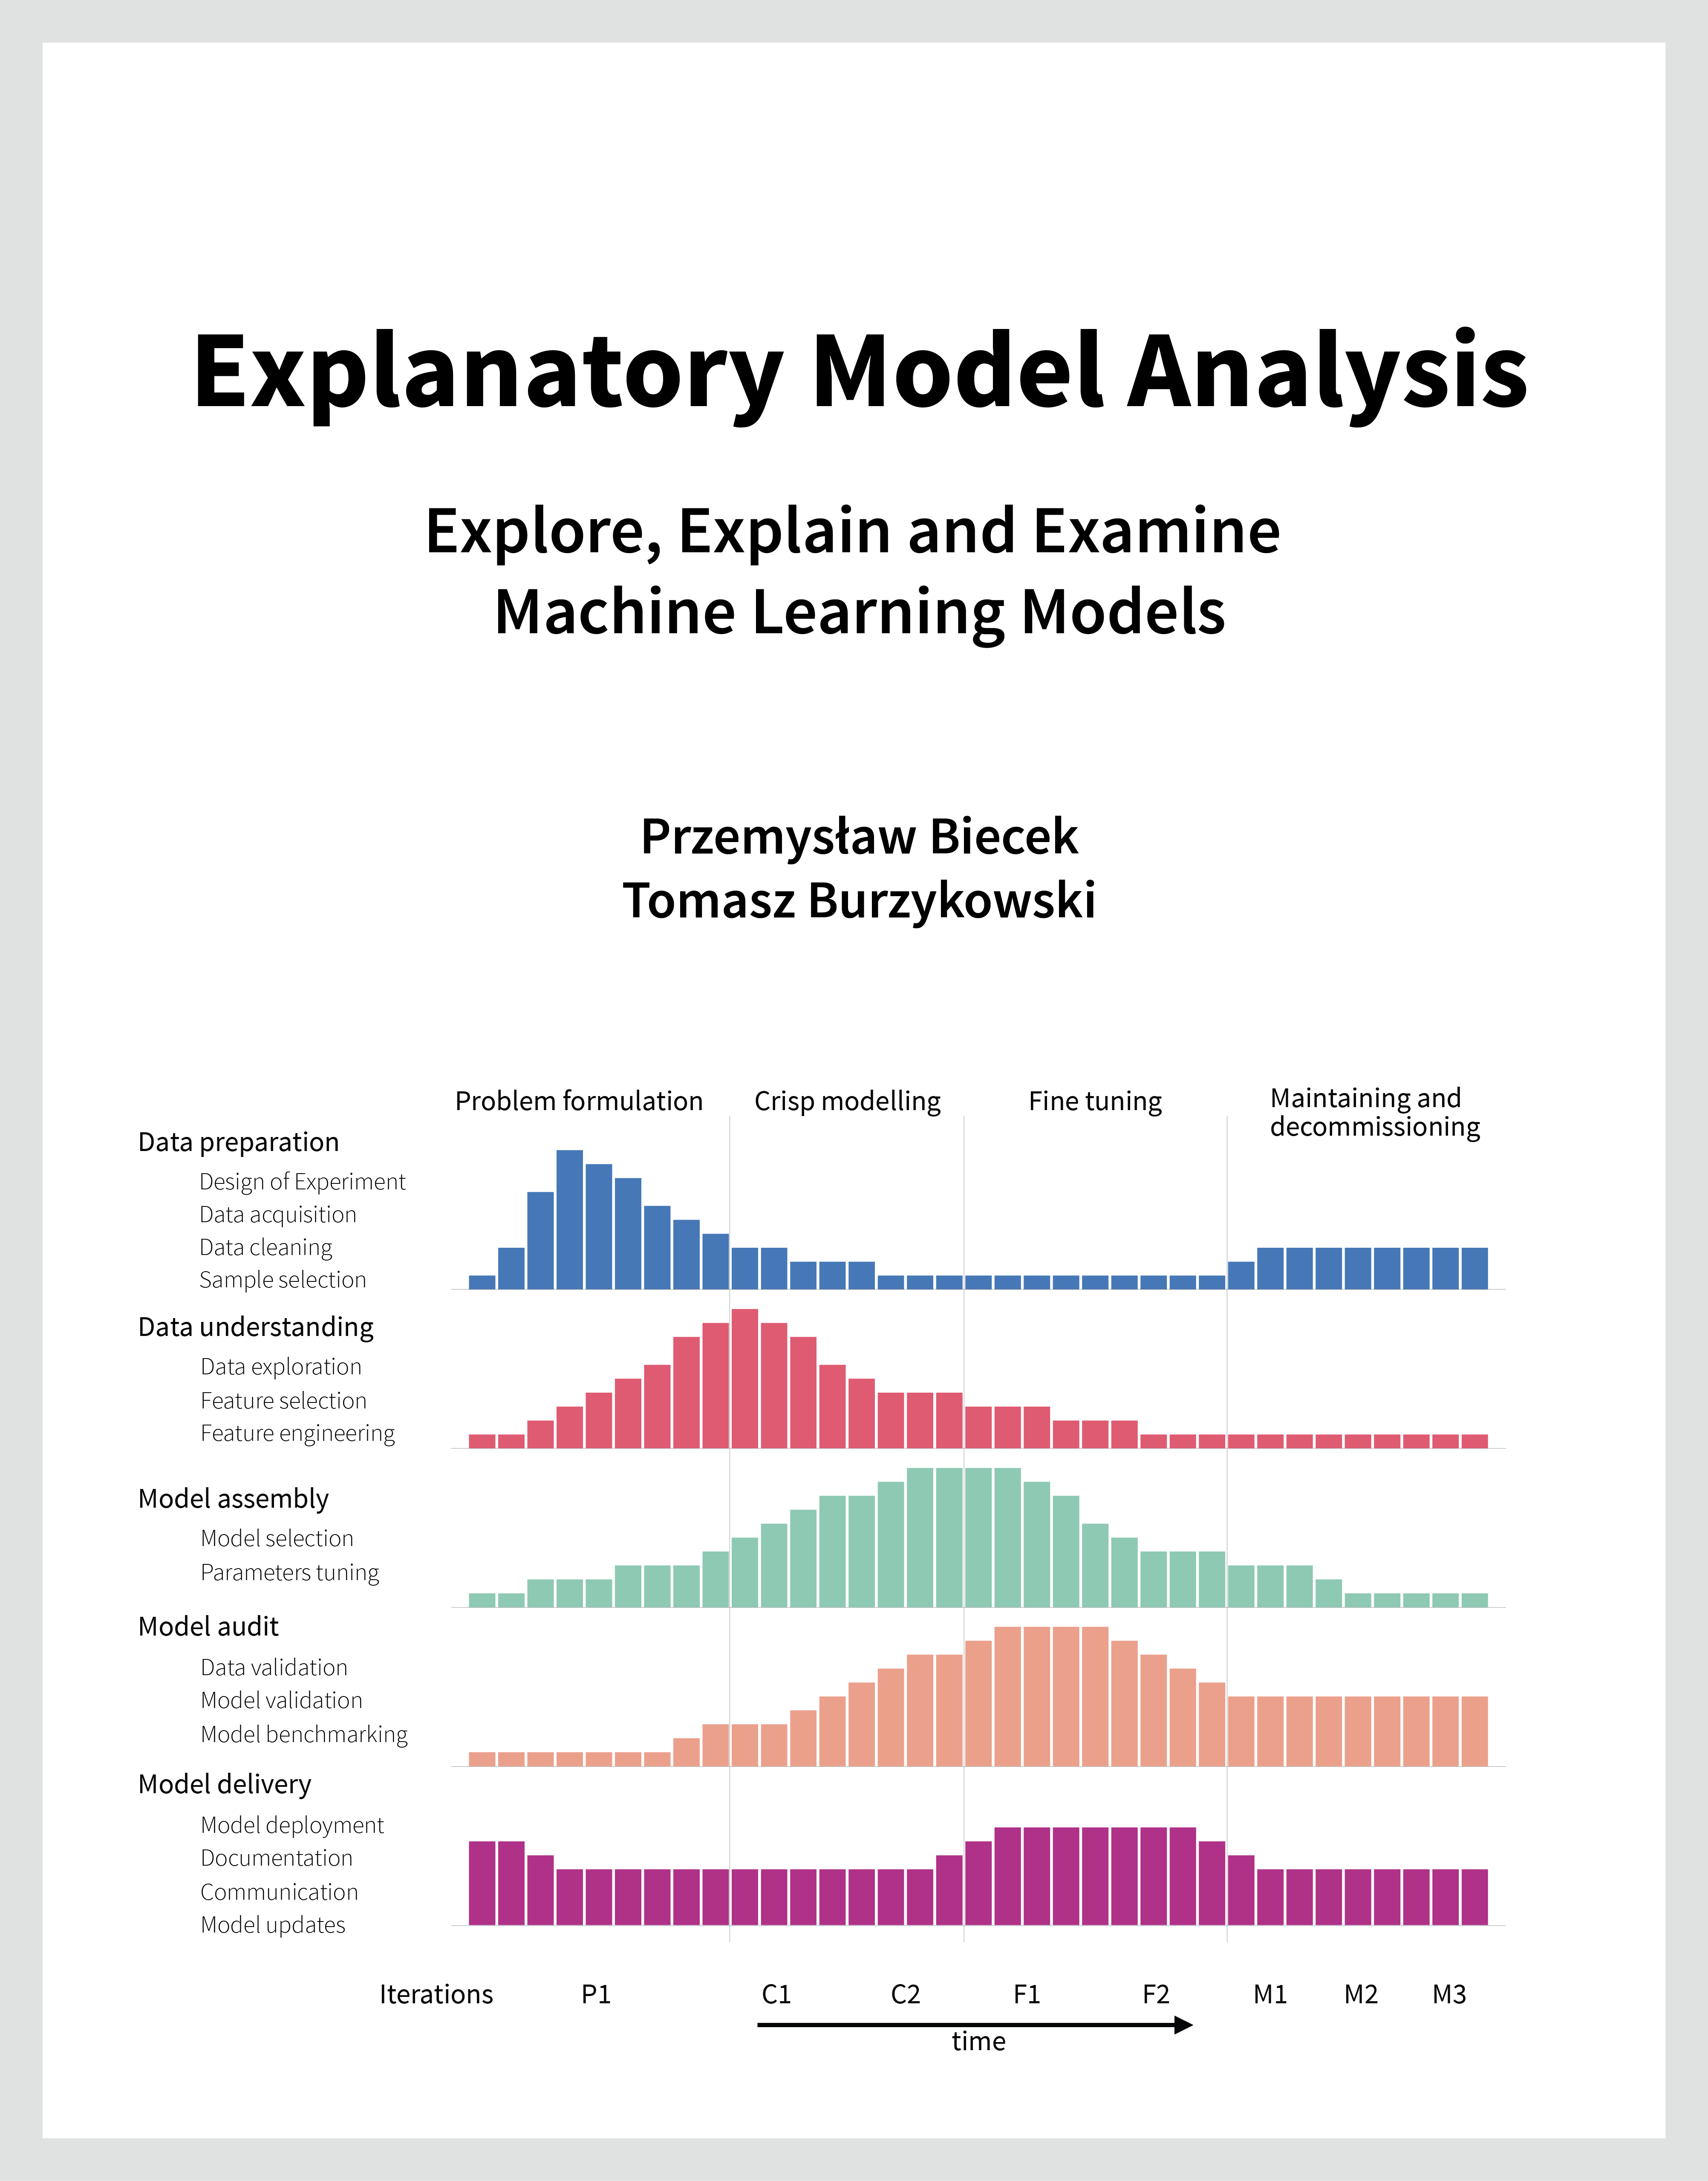
\includegraphics[width=0.99\linewidth]{figure/front} \end{center}

\hypertarget{introduction}{%
\section{Introduction}\label{introduction}}

\hypertarget{notes-to-readers}{%
\subsection{Notes to readers}\label{notes-to-readers}}

A note to readers: this text is a work in progress.

We've released this initial version to get more feedback. Feedback can
be given at the GitHub repo
\url{https://github.com/pbiecek/PM_VEE/issues}. Copyediting has not been
done yet so read at your own risk.

We are primarily interested in the organization and consistency of the
content, but any comments will be welcommed.

Thanks for taking the time to read this.

We'd like to thank everyone that contributed feedback, typos, or
discussions while the book was being written. GitHub contributors
included, \href{https://github.com/agosiewska/}{agosiewska}, Rees
Morrison.

\hypertarget{the-aim-of-the-book}{%
\subsection{The aim of the book}\label{the-aim-of-the-book}}

Predictive models are used to guess (statisticians would say: predict)
values of a variable of interest based on other variables. As an
example, consider prediction of sales based on historical data,
prediction of risk of heart disease based on patient characteristics, or
prediction of political attitudes based on Facebook comments.

Predictive models have been constructed through the enitre human
history. Ancient Egyptians, for instance, used observations of the
rising of Sirius to predict flooding of the Nile. A more rigorous
approach to model construction may be attributed to the method of least
squares, published more than two centuries ago by Legendre in 1805 and
by Gauss in 1809. With time, the number of applications in economy,
medicine, biology, and agriculture has grown. The term \emph{regression}
was coined by Francis Galton in 1886. Initially, it was referring to
biological applications, while today it is used for various models that
allow prediction of continuous variables. Prediction of nominal
variables is called \emph{classification}, and its beginning may be
attributed to works of Ronald Fisher in 1936.

During the last century, many statistical models that can be used for
predictive purposes have been developed. These include linear models,
generalized linear models, regression and classification trees,
rule-based models, and many others. Developments in mathematical
foundations of predictive models were boosted by increasing
computational power of personal computers and availability of large
datasets in the era of ,,big data'' that we have entered.

With the increasing demand for predictive models, model features such as
flexibility, ability to perform internally variable selection (feature
engineering), and high precision of predictions are of interest. To
obtain robust models, ensembles of models are used. Techniques like
bagging, boosting, or model stacking combine hundreds or thousands of
small models into a one super-model. Large deep neural models have over
a billion parameters.

There is a cost of this progress. Complex models may seem to operate
like ,,black boxes'`. It may be difficult, or even impossible, to
understand how thousands of coefficients affect the model prediction. At
the same time, complex models may not work as well as we would like them
to. An overview of real problems with large black-box models may be
found in an excellent book of Cathy O'Neil \citep{ONeil} or in her TED
Talk ,,\emph{The era of blind faith in big data must end}''. There is a
growing number of examples of predictive models with performance that
deteriorated over time or became biased in some sense. For instance,
IBM's Watson for Oncology was criticized by oncologists for delivering
unsafe and inaccurate recommendations \citep{IBMWatson}. Amazon's system
for CV screening was found to be biased against women \citep{AmazonAI}.
The COMPAS (Correctional Offender Management Profiling for Alternative
Sanctions) algorithm for predicting recidivism, developed by Northpointe
(now Equivant), is biased against blacks \citep{COMPAS}. These are
examples of models and algorithms that led to serious violations of
fairness and ethical principles. An example of situation when data drift
led to deterioration in model performance is the Google Flu model, which
gave worse predictions after two years than at baseline
\citep{GoogleFLU}, {[}Lazer et al Science 2014{]}.

A reaction to some of these examples and problems are new regulations,
like the General Data Protection Regulation \citep{EUGDPR}. Also, new
civic rights are being formulated \citep{RightToExpl},
\citep{RightToExpl2}, \citep{RightToExpl3}. A noteworthy example is the
\emph{,,Right to Explanation''}, i.e., the right to be provided an
explanation for an output of an automated algorithm \citep{RightToExpl}.
To exercise the right, methods for verification, exploration, and
explanation of predictive models are needed.

We can conclude that, today, the true bottleneck in predictive modelling
is not the lack of data, nor the lack of computational power, nor
inadequate algorithms, nor the lack of flexible models. It is the lack
of tools for model validation, model exploration, and explanation of
model decisions. Thus, in this book, we present a collection of methods
that may be used for this purpose. As development of such methods is a
very active area of research and new methods become available almost on
a continuous basis, we do not aim at being exhaustive. Rather, we
present the mind-set, key problems, and several examples of methods that
can be used in model exploration.

\begin{figure}

{\centering 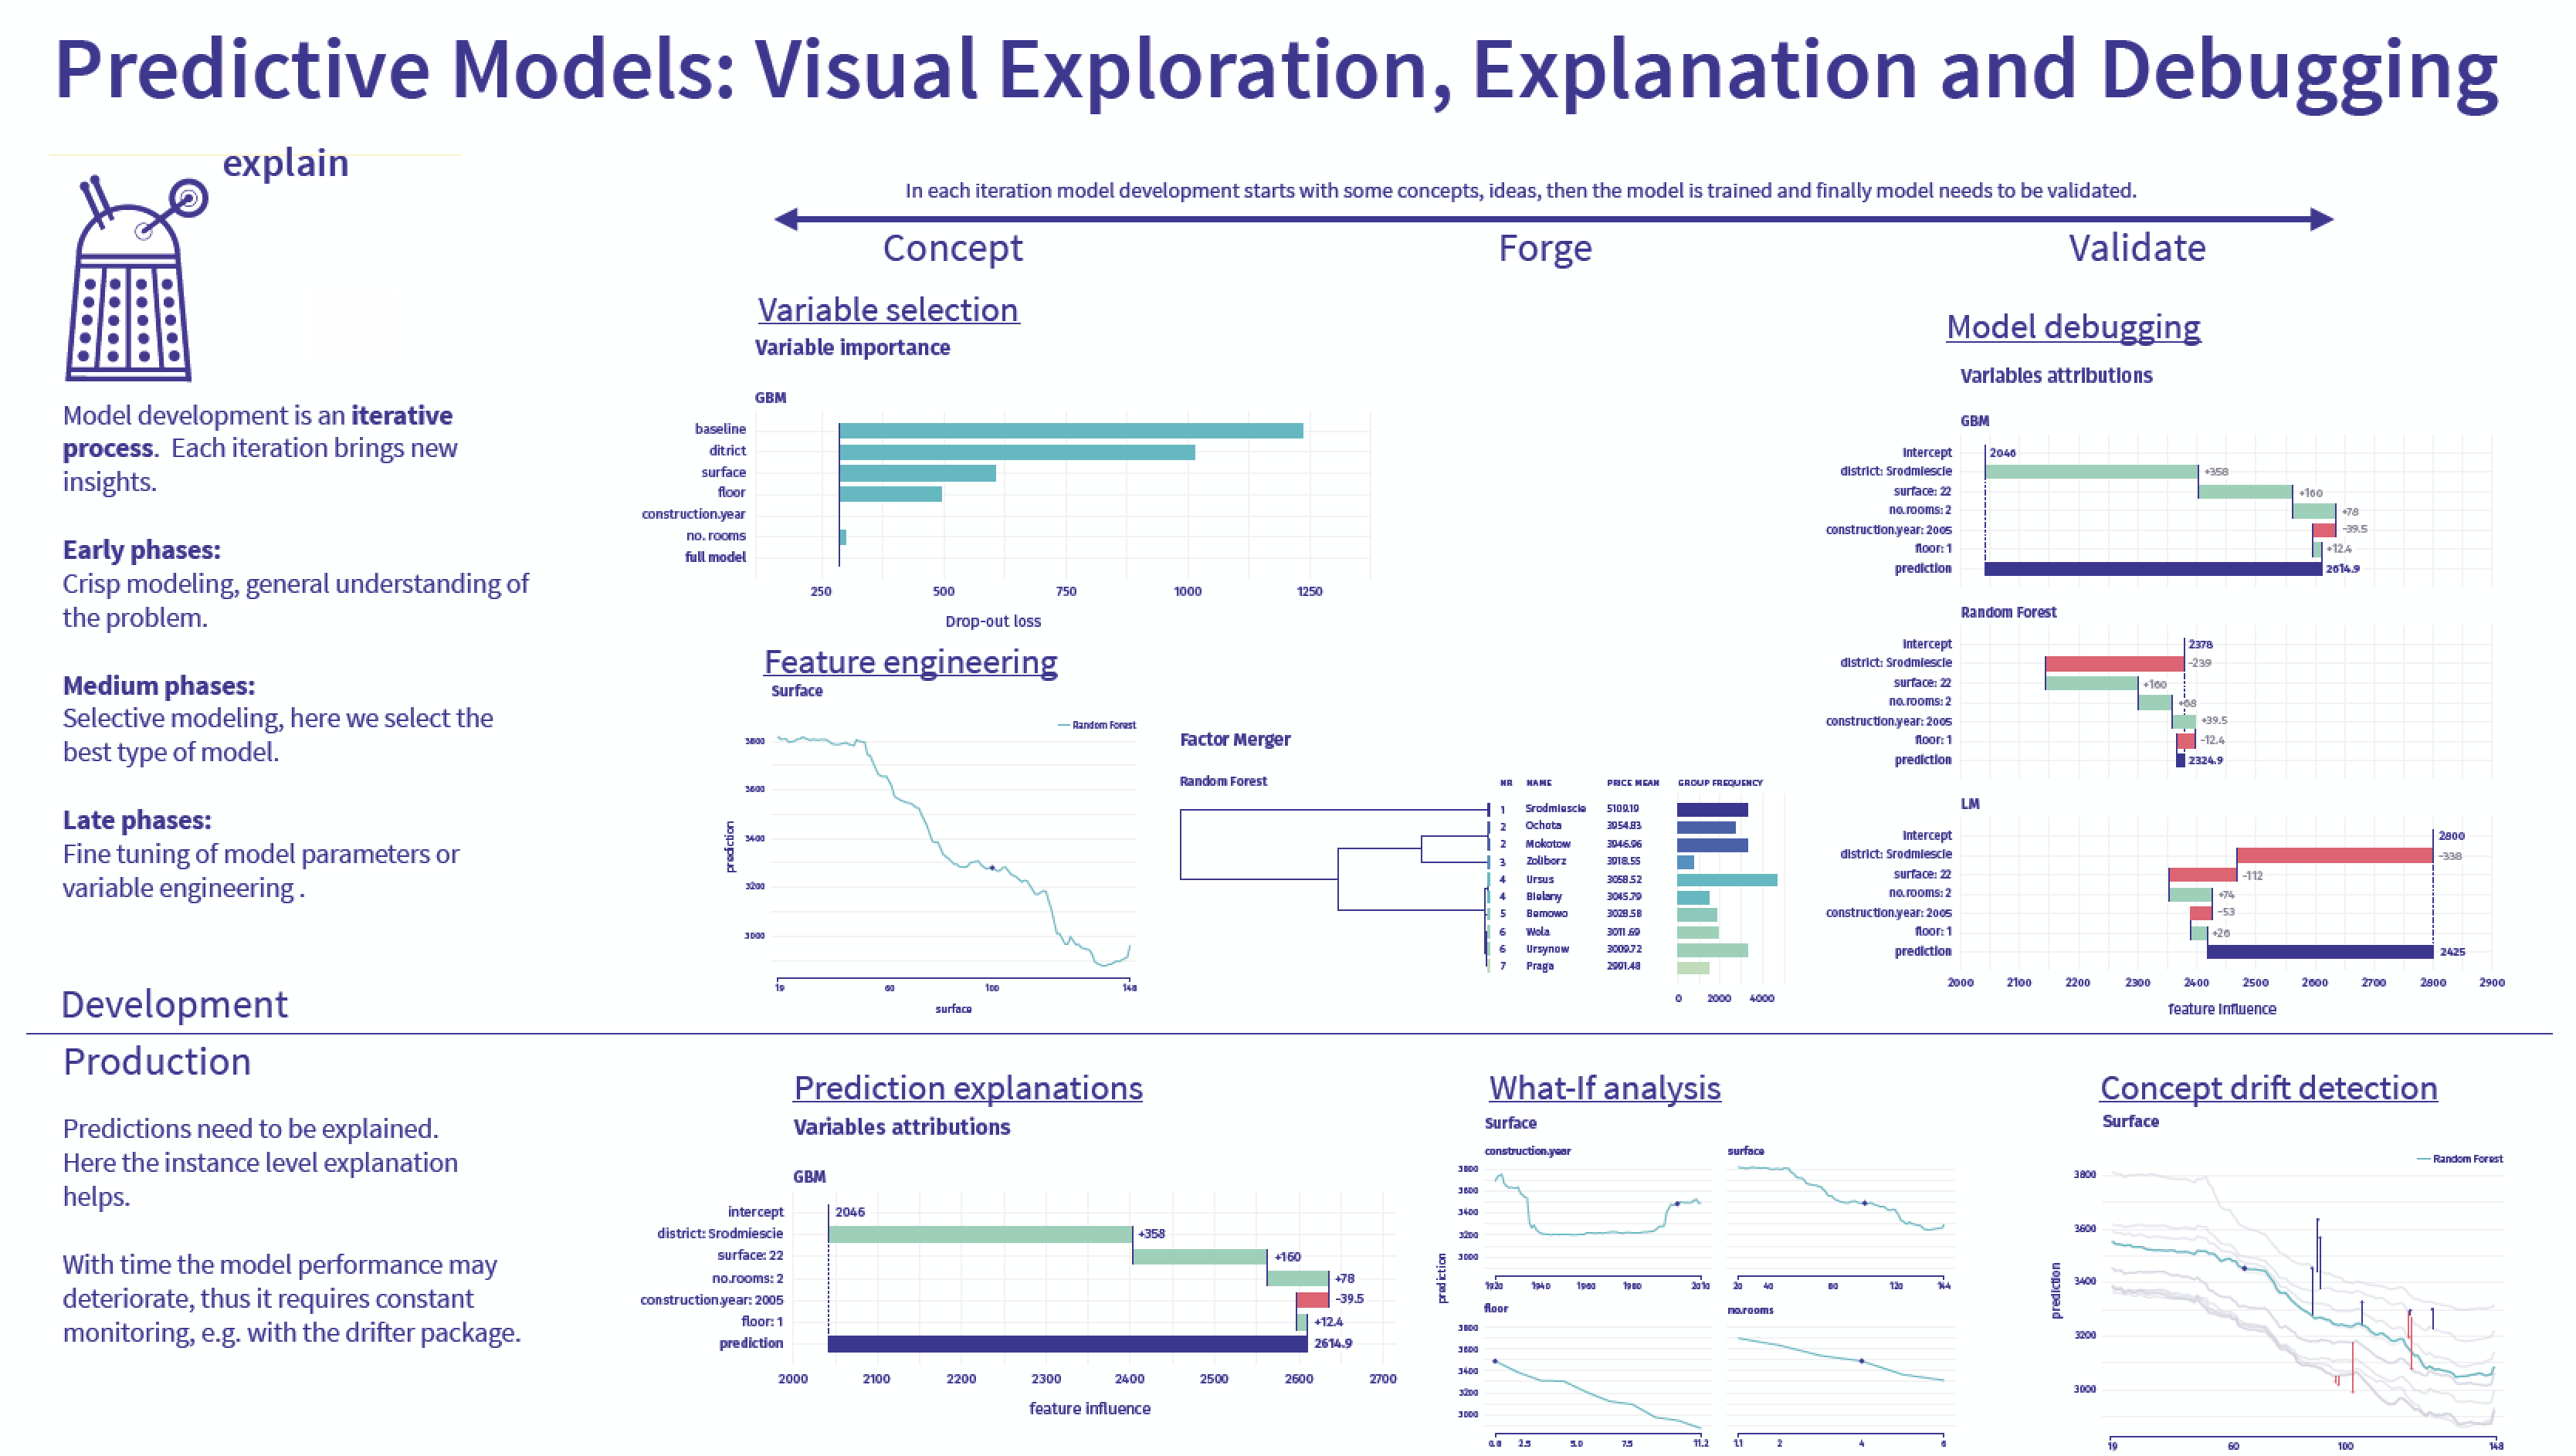
\includegraphics[width=0.99\linewidth]{figure/DrWhyAI_PMVEE} 

}

\caption{(fig:DrWhyAIPMVEE) Visual exploration of predictive models help in every phase of model life-cycle. Model level methods help in early crisp modeling. Instance level methods help in debugging. Feature effects help to cross-compare candidate models. Auditors help to identify weak sides of considered models.}\label{fig:DrWhyAIPMVEE}
\end{figure}

\hypertarget{three-single-laws}{%
\subsection{A bit of philosophy: three laws of model
explanation}\label{three-single-laws}}

Seventy-six years ago, Isaac Asimov forumlated
\href{https://en.wikipedia.org/wiki/Three_Laws_of_Robotics}{Three Laws
of Robotics}: 1) a robot may not injure a human being, 2) a robot must
obey the orders given it by human beings, and 3) a robot must protect
its own existence.

Today's robots, like cleaning robots, robotic pets, or autonomous cars
are far from being conscious enough to fall under Asimov's ethics.
However, we are more and more surrounded by complex predictive models
and algorithms used for decision making. Machine-learning models are
used in health care, politics, education, justice, and many other areas.
The models and algorithms have a far larger influence on our lives than
physical robots. Yet, applications of such models are left unregulated
despite examples of their potential harmfulness. See \emph{Weapons of
Math Destruction} by Cathy O'Neil \citep{ONeil} for an excellent
overview of selected problems.

It's clear that we need to control the models and algorithms that may
affect us. Thus, Asimov's laws are referred to in the context of the
discussion around
\href{https://en.wikipedia.org/wiki/Ethics_of_artificial_intelligence}{Ethics
of Artifical Intelligence}. Initiatives to formulate principles for AI
development have been undertaken, for instance, in the UK {[}Olhede \&
Wolfe, Significance 2018, 15: 6-7{]}. Following Asimov's approach, we
propose three requirements that any predictive model should fulfill:

\begin{itemize}
\tightlist
\item
  \textbf{Prediction's justification}. For every prediction of a model,
  one should be able to understand which variables affect the prediction
  and to what extent.
\item
  \textbf{Prediction's speculation}. For every prediction of a model,
  one should be able to understand how the model prediction would change
  if input variables changed.
\item
  \textbf{Prediction's validation}. For every prediction of a model, one
  should be able to verify how strong is the evidence that confirms the
  prediction.
\end{itemize}

We see two ways to comply with these requirements. One is to use only
models that fulfill these conditions by design. However, the price for
transparency may be a reduction in performance. Another way is to use
tools that allow, perhaps by using approximations, to ,,explain''
predictions for any model. In our book, we will focus on the latter
approach.

\hypertarget{terminology}{%
\subsection{Terminology}\label{terminology}}

It is worth noting that, when it comes to predictive models, the same
concepts have often been given different names in statistics and in
machine learning. For instance, in the statistical-modelling literature,
one refers to ,,explanatory variables,'' with ,,independent variables,''
,,predictors,'' or ,,covariates'' as often-used equivalents. Explanatory
variables are used in the model as means to explain (predict) the
,,dependent variable,'' also called ,,predicted'' variable or
,,response.'' In machine-learning terminology, ,,input variables'' or
,,features'' are used to predict the ,,output'' variable. In statistical
modelling, models are fit to the data that contain ,,observations,''
whereas in the machine-learning world a dataset may contain
,,instances.''

To the extent possible, in our book we try to consistently use the
statistical-modelling terminology. However, the reader may find
references to a ,,feature'' here and there. Somewhat inconsistently, we
also introduce the term ,,instance-level'' explanation. Instance-level
explanation methods are designed to extract information about the
behavior of the model related to a specific observation (or instance).
On the other hand, ,,global'' explanation techniques allow obtaining
information about the behavior of the model for an entire dataset.

We consider models for dependent variables that can be continuous or
nominal. The values of a continuous variable can be represented by
numbers with an ordering that makes some sense (zip codes or phone
numbers are not considered as continuous variables). A continuous
variable does not have to be continuous in the mathematical sense;
counts (number of floors, steps, etc.) will be treated as continuous
variables as well. A nominal variable can assume only a finite set of
values that cannot be given numeric values.

In this book we focus on ,,black-box'' models. We discuss them in a bit
more detail in the next section.

\hypertarget{glass-box-models-vs.black-box-models}{%
\subsection{Glass-box models vs.~black-box
models}\label{glass-box-models-vs.black-box-models}}

Black-box models are models with a complex structure that is hard to
understand by humans. Usually this refers to a large number of model
coefficients. As people vary in their capacity to understand complex
models, there is no strict threshold for the number of coefficients that
makes a model a black-box. In practice, for most people this threshold
is probably closer to 10 than to 100.

A ,,glass-box'' (sometimes called white-box) model, which is opposite to
a ,,black-box'' one, is a model that is easy to understand (though maybe
not by every pearson). It has a simple structure and a limited number of
coefficients. The two most common classess of glass-box models are
decision or regression trees, as an example in Figure \ref{fig:BILLCD8},
or models with an additive structure, like the following model for
mortality risk in melanoma patients:

\[
RelativeRisk = 1 + 3.6 * [Breslow > 2] - 2 * [TILs > 0] 
\]

In the model, two explanatory variables are used: an indicator whether
the thickness of the lesion according to the Breslow scale is larger
than 2 mm and an indicator whether the percentage of tumor-infiltrating
lymphocytes (TILs) is larger than 0.

The structure of a glass box-model is, in general, easy to understand.
It may be difficult to collect the necessary data, build the model, fit
it to the data, or perform model validation, but once the model has been
developed its interpretation and mode of working is straightforward.

Why is it important to understand the model structure? There are several
important advantages. If the model structure is clear, we can easily see
which variables are included in the model and which are not. Hence, for
instance, we may be able to, question the model when a particular
explanatory variable was excluded from it. Also, in the case of a model
with a clear structure and a limited number of coefficients, we can
easily link changes in model predictions with changes in particular
explanatory variables. This, in turn, may allow us to challenge the
model against domain knowledge if, for instance, the effect of a
particular variable on predictions is inconsistent with previously
established results. Note that linking changes in model predictions with
changes in particular explanatory variables may be difficult when there
are many variables and/or coefficients in the model. For instance, a
classification tree with hundreds of nodes is difficult to understand,
as is a linear regression model with hundreds of cofficients.

Comprehending the performance of a black-box models presents more
challenges. The structure of a complex model, such as a neural-network
model, mmay be far from transparent. Consequently, we may not understand
which features influence the model decisions and bby how much.
Consequently, it may be difficult to decide whether the model is
consistent with our domain knowledge. In our book we present tools that
can help in extracting the information necessary for the evaluation of
complex models.

\begin{figure}

{\centering 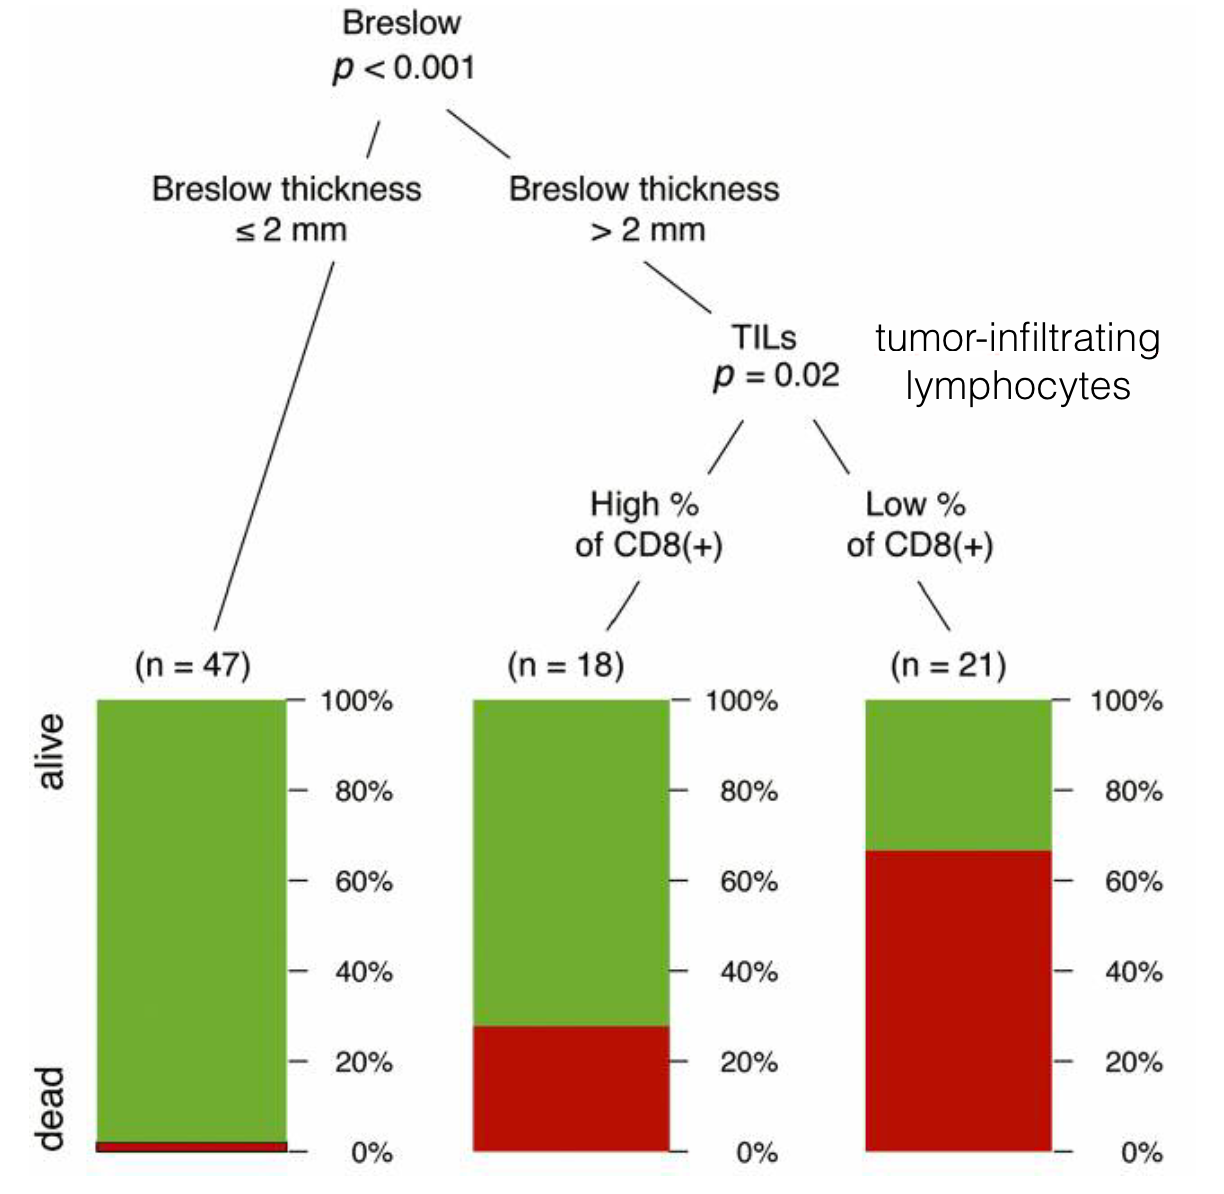
\includegraphics[width=0.5\linewidth]{figure/wbBILL8model} 

}

\caption{(fig:BILLCD8) Example tree model for melanoma risk}\label{fig:BILLCD8}
\end{figure}

\hypertarget{model-visualization-exploration-and-explanation}{%
\subsection{Model visualization, exploration, and
explanation}\label{model-visualization-exploration-and-explanation}}

In general, the lifecycle of a model can be divided, into three phases:
development (or building), deployment, and maintenance.

Model development is the phase in which one is looking for the best
available model. During this process, model exploration tools are
useful. Exploration involves evaluation of the fit of the model,
verification of the assumptions underlying the model (diagnostics), and
assessment of the predictive performance of the model (validation). In
our book we will focus on the visualization tools that can be useful in
model exploration. We will not, however, discuss visualization methods
for diagnostic purposes, as they are extensively discussed in many books
devoted to statistical modelling.

Model deployment is the phase in which a predictive model is adopted for
use. In this phase, it is crucial that the users gain confidence in
using the model. It is worth noting that the users might not have been
involved in the model development. Moreover, they may only have access
to the binary implementation of the model, may not provide any insight
into the details of the model structure. In this situation, model
explanation tools can help to understand the factors that influence
model predictions and boost confidence in the model. The tools are one
of the main focus points of our book.

Finally, a deployed model requires maintenance. In this phase, one
monitors a model performance by, for instance, checking the validity of
predictions for different datasets. If issues are detected, model
explanation tools may be used to find the source of the problem and to
suggest a modification of the structure of the model.

\hypertarget{model-agnostic-vs.model-specific-approach}{%
\subsection{Model-agnostic vs.~model-specific
approach}\label{model-agnostic-vs.model-specific-approach}}

Some classes of models have been developed for a long period of time or
have attracted intensive research. Consequently, those classes of models
are equipped with excellent tools for model exploration or
visualisation. For example:

\begin{itemize}
\tightlist
\item
  There are many tools for diagnostics and evaluation of linear models.
  Model assumptions are formally defined (normality, linear structure,
  homogenous variance) and can be checked by using normality tests or
  plots (normal qq-plot), diagnostic plots, tests for model structure,
  tools for identification of outliers, etc.
\item
  For many more advanced models with an additive structure, like the
  proportional hazards model, many tools can be used for checking model
  assumptions.
\item
  Random-forest models are equipped with the out-of-bag method of
  evaluating performance and several tools for measuring variable
  importance \citep{R-randomForest}. Methods have been developed to
  extract information from the model structure about possible
  interactions \citep{R-randomForestExplainer}. Similar tools have been
  developed for other ensembles of trees, like xgboost models
  \citep{R-xgboostExplainer}.
\item
  Neural networks enjoy a large collection of dedicated
  model-explanation tools that use, for instance, the layer-wise
  relevance propagation technique \citep{BachLWRP}, or saliency maps
  technique \citep{SaliencyMaps}, or a mixed approach.
\end{itemize}

Of course, the list of model classes with dedicated collections of
model-explanation and/or diagnostics methods is much longer. This
variety of model-specific approaches does lead to issues, though. For
instance, one cannot easily compare explanations for two models with
different structures. Also, every time a new architecture or a new
ensemble of models is proposed, one needs to look for new methods of
model exploration. Finally, for brand-new models no tools for model
explanation or diagnostics may be immediately available.

For these reasons, in our book we focus on model-agnostic techniques. In
particular, we prefer not to assume anything about the model structure,
as we may be dealing with a black-box model with an unclear structure.
In that case, the only operation that we may be able to perform is
evaluation of a model for a selected observation.

However, while we do not assume anything about the structure of the
model, we will assume that the model operates on \(p\)-dimensional
vectors and, for a single vector, it returns a single value which is a
real number. This assumption holds for a broad range of models for data
such as tabular data, images, text data, videos, etc. It may not be
suitable for, e.g., models with memory like seq2seq models
\citep{seq2seq} or Long Short Term Memory models \citep{lstm} in which
the model output depends also on sequence of previous inputs.

\hypertarget{notation}{%
\subsection{Notation}\label{notation}}

Methods described in this book were developed by different authors, who
used different mathematical notations. We try to keep the mathematical
notation consistent throughout the entre book. In some cases this may
result in formulae wth a fairly complex system of indices.

In this section, we provide a general overview of the notation we use.
Whenever necessary, parts of the notation will be explained again in
subsequent chapters.

We consider predictive models that operate on a \(p\)-dimensional input
space \(\mathcal X\). By \(x \in \mathcal X\) we will refer to a single
point in this input space.

In some cases models are described in context of a dataset with \(n\)
observations. By \(x_i\) we refer to the \(i\)-th observation in this
dataset. Of course, \(x_i \in \mathcal X\).

Some explainers are constructed around an observation of interest which
will be denoted by \(x_{*}\). The observation may not necessarily belong
to the analyzed dataset; hence, the use of the asterisk in the index. Of
course, \(x_* \in \mathcal X\).

Points in \(\mathcal X\) are \(p\) dimensional vectors. We will refer to
the \(j\)-th coordinate by using \(j\) in superscript. Thus, \(x^j_i\)
deontes the \(j\)-th coordinate of the \(i\)-th observation from the
analyzed dataset. If \(\mathcal J\) denotes a subset of indices, then
\(x^{\mathcal J}\) denotes the elements of vector \(x\) corresponding to
the indices included in \(\mathcal J\).

We will use the notation \(x^{-j}\) to refer to a vector that results
from removing the \(j\)-th coordinate from vector \(x\). By
\(x^{j|=z}\), we denote a vector with the values at all coordinates
equal to the values in \(x\), except of the \(j\)-th coordinate, which
is set equal to \(z\). So, if \(w=x^{j|=z}\), then \(w^j = z\) and
\(\forall_{k\neq j} w^k = x^k\).

In this book, a model is a function \(f:\mathcal X \rightarrow y\) that
transforms a point from \(\mathcal X\) into a real number. In most
cases, the presented methods can be used directly for multi-variate
dependent variables; however, we use examples with uni-variate responses
to simplify the notation.

We will use \(r_i = y_i - f(x_i)\) we refer to the model residual, i.e.,
the difference between the observed value of the dependent variable
\(Y\) for the \(i\)-th observation from a particular dataset and the
model prediction for the observaton.

\hypertarget{bookstructure}{%
\subsection{The structure of the book}\label{bookstructure}}

Our book is split in two parts. In the part \emph{Instance-level
explainers}, we present techniques for exploration and explanation of
model predictions for a single observation. On the other hand, in the
part \emph{Global explainers}, we present techniques for exploration and
explanation of model's performance for an entire dataset.

Before embarking on the description of the methods, in Chapter
\ref{doItYourselfWithR}, we provide a short description of R tools and
packages that are necessary to replicate the results presented for
various methods. In Chapter \ref{dataSetsIntro}, we describe three
datasets that are used throughout the book to illustrate the presented
methods and tools.

The \emph{Instance-level explainers} part of the book consists of
Chapters \ref{ceterisParibus}-\ref{SummaryInstanceLevel}. In Chapters
\ref{ceterisParibus}-\ref{localDiagnostics}, methods based on
Ceteris-paribus (CP) profiles are presented. The profiles show the
change of model-based predictions induced by a change of a single
variable; they are introduced in Chapter \ref{ceterisParibus}. Chapter
\ref{ceterisParibusOscillations} presents a CP-profile-based measure
that summarizes the impact of a selected variable on model's
predictions. The measure can be used to select the profiles that are
worth plotting for a model with a large number of explanatory variables.
Chapter \ref{localDiagnostics} describes local-fidelity plots that are
useful to investigate the sources of a poor prediction for a particular
single observation.

Chapters \ref{breakDown}-\ref{shapley} present methods to decompose
variable contributions to model predictions. In particular, Chapter
\ref{breakDown} introduces Break-down (BD) plots for models with
additive effects. On the other hand, Chapter \ref{iBreakDown} presents a
method for models including interactions. Finally, Chapter \ref{shapley}
describes an alternative method for decomposing model predictions that
is closely linked with Shapley values \citep{shapleybook1952} developed
originally for cooperative games.

Chapter \ref{LIME} presens a different approach to explanation of
single-instance predictions. It is based on a local approximation of a
black-box model by a simpler, glass-box one. In paricular, in the
chapter, the Local Interpretable Model-Agnostic Explanations (LIME)
method \citep{lime} is discussed.

The final chapter of the first part, Chapter \ref{SummaryInstanceLevel},
presence a comparison of various instance-level explainers.

The \emph{Global explainers} part of the book consists of Chapters
\ref{ModelLevelExploration}-\ref{conceptDrift}.

In each part, every method is described in a separate chapter that has
the same structure: * Subsection \emph{Introduction} explains the goal
of and the general idea behind the method. * Subsection \emph{Method}
shows mathematical or computational details related to the method. This
subsection can be skipped if you are not interested in the details. *
Subsection \emph{Example} shows an exemplary application of the method
with discussion of results. * Subsection \emph{Pros and cons} summarizes
the advantages and disadvantages of the method. It also provides some
guideance regarding when to use the method. * Subsection \emph{Code
snippets} shows the implementation of the method in R and Python. This
subsection can be skipped if you are not interested in the
implementation.

Finally, we would like to signal that, \textbf{in this book, we do show}

\begin{itemize}
\tightlist
\item
  how to determine features that affect model prediction for a single
  observation. In particular, we present the theory and examples of
  methods that can be used to explain prediction like break down plots,
  ceteris paribus profiles, local-model approximations, or Shapley
  values.
\item
  techniques to examine fully-trained machine-learning models as a
  whole. In particular, we review the theory and examples of methods
  that can be used to explain model performance globally, like
  partial-dependency plots, variable-importance plots, and others.
\item
  charts that can be used to present key information in a quick way.
\item
  tools and methods for model comparison.
\item
  code snippets for R and Python that explain how to use the described
  methods.
\end{itemize}

On the other hand, \textbf{in this book, we do not focus on}

\begin{itemize}
\tightlist
\item
  any specific model. The techniques presented are model agnostic and do
  not make any assumptions related to model structure.
\item
  data exploration. There are very good books on this topic, like R for
  Data Science \url{http://r4ds.had.co.nz/} or TODO
\item
  the process of model building. There are also very good books on this
  topic, see An Introduction to Statistical Learning by Gareth James,
  Daniela Witten, Trevor Hastie and Robert Tibshirani
  \url{http://www-bcf.usc.edu/~gareth/ISL/} or TODO
\item
  any particular tools for model building. These are discussed, for
  instance, in Applied Predictive Modeling by Max Kuhn and Kjell Johnson
  \url{http://appliedpredictivemodeling.com/}
\end{itemize}

\hypertarget{thanksto}{%
\subsection{Acknowledgements}\label{thanksto}}

Przemek's work on interpretability started during research trips within
the RENOIR project (691152 - H2020/2016-2019). So he would like to thank
Prof.~Janusz Holyst for the chance to take part in this project.

Przemek would also like thank Prof.~Chris Drake for her hospitality.
This book would have never been created without perfect conditions that
Przemek found at Chris's house in Woodland.

This book has been prepared using the \textbf{bookdown} package
\citep{R-bookdown}, created thanks to the amazing work of Yihui Xie.

\hypertarget{doItYourselfWithR}{%
\section{Do-it-yourself With R}\label{doItYourselfWithR}}

In our book we introduce different methods for instance-level and global
explanation and exploration of predictive models. In each chapter, there
is a section with code snippets for R that show how a particular method
has been implemented. In this chapter we provide a short description of
steps that will allow the reader to replicate the results presented for
various methods.

\hypertarget{what-to-install}{%
\subsection{What to install?}\label{what-to-install}}

Obviously, R \citep{RcoreT} is needed. It is always better to use the
newest version, but at least R in version 3.5 should be used. R can be
downloaded from \url{https://cran.r-project.org/}.

A good editor makes working with R much easier. There is a plenty of
choices, but, especially for beginners, it is worth considering the
RStudio editor, an open-source and enterprise-ready tool for R. It can
be downloaded from \url{https://www.rstudio.com/}.

Once R and the editor are available, the required packages should be
installed.

The most important one is the \texttt{DALEX} package. It is the entry
point to solutions introduced in this book. The package can be installed
by executing the following command from the R command line:

\begin{verbatim}
install.packages("DALEX")
\end{verbatim}

Installation of \texttt{DALEX} will automatically take care about
installation of other hard requirements (packages required by it), like
the \texttt{ggplot2} package for data visualization.

To repeat all examples in this book, two additional packages are needed:
\texttt{ingredients} and \texttt{iBreakDown}. The easiest way to get
them, including other useful weak dependencies, is to execute the
following command:

\begin{verbatim}
DALEX::install_dependencies()
\end{verbatim}

\hypertarget{how-to-work-with-dalex}{%
\subsection{\texorpdfstring{How to work with
\texttt{DALEX}?}{How to work with DALEX?}}\label{how-to-work-with-dalex}}

To conduct model exploration with \texttt{DALEX}, first, a model has to
be created. Then the model has got to be prepared for exploration.

There are many packages in R that can be used to construct a model. Some
packages are structure-specific, like \texttt{randomForest} for
Random-Forest Classification and Regression models \citep{randomForest},
\texttt{gbm} for Generalized Boosted Regression Models \citep{gbm},
extensions for Generalized Linear Models \citep{rms}, or many others.
There is also a number of packages that can be used for constucting
models with different structures. These include the \texttt{h2o} package
\citep{h2oPackage}, \texttt{caret} \citep{caret} and its successor
\texttt{parsnip} \citep{parsnipPackage}, a very powerful and extensible
\texttt{mlr} \citep{mlr}, or \texttt{keras} that is a wrapper to Python
library with the same name \citep{kerasPackage}.

While it is great to have such a large choice of tools for constructing
models, the downside is that different packages have different
interfaces and different arguments. Moreover, model-objects created with
different packages may have different internal structures. The main goal
of the \texttt{DALEX} package \citep{R-DALEX} is to create a level of
abstraction around a model that makes it easier to explore and explain
the model.

Function \texttt{DALEX::explain} is THE function for model wrapping. The
function requires five arguments:

\begin{itemize}
\tightlist
\item
  \texttt{model}, a model-object;
\item
  \texttt{data}, a data frame with validation data;
\item
  \texttt{y}, observed values of the dependent variable for the
  validation data; it is an optional argument, required for explainers
  focused on model validation and benchmarking.
\item
  \texttt{predict\_function}, a function that returns prediction scores;
  if not specified, then a default \texttt{predict()} function is used.
  Note that, for some models, the default \texttt{predict()} function
  returns classes; in such cases you should provide a function that will
  return numerical scores.
\item
  \texttt{label}, a name of a model; if not specified, then it is
  extracted from the \texttt{class(model)}. This name will be presented
  in figures, so it is recommended to make the name informative.
\end{itemize}

For an example, see Section \ref{ExplainersTitanicRCode}.

\hypertarget{how-to-work-with-archivist}{%
\subsection{\texorpdfstring{How to work with
\texttt{archivist}?}{How to work with archivist?}}\label{how-to-work-with-archivist}}

As we will focus on exploration of predictive models, we prefer not to
waste space nor time on replication of the code necessary for model
development. This is where the \texttt{archivist} packages helps.

The \texttt{archivist} package \citep{archivist} is designed to store,
share, and manage R objects. We will use it to easily access R models
and explainers. To install the package, the following command should be
executed in the R command line:

\begin{verbatim}
install.packages("archivist")
\end{verbatim}

Once the package has been installed, function \texttt{aread()} can be
used to retrieve R objects from any remote repository. For this book, we
use a GitHub repository \texttt{models} hosted at
\url{https://github.com/pbiecek/models}. For instance, to download a
model with the md5 hash \texttt{ceb40}, the following command has to be
executed:

\begin{Shaded}
\begin{Highlighting}[]
\NormalTok{archivist}\OperatorTok{::}\KeywordTok{aread}\NormalTok{(}\StringTok{"pbiecek/models/ceb40"}\NormalTok{)}
\end{Highlighting}
\end{Shaded}

Since the md5 hash \texttt{ceb40} uniquely defines the model, referring
to the repository object results in using exactly the same model and the
same explanations. Thus, in the subsequent chapters, pre-constructed
model explainers will be accessed with \texttt{archivist} hooks.

\hypertarget{Packages}{%
\subsection{DrWhy Packages}\label{Packages}}

Here we present list of arguments in explainers from \texttt{DrWhy}
universe. All explainers use unified set of arguments. All of them are
generic with two specific implementations \texttt{*.explainer} and
\texttt{*.default}. The first one is working for objects created with
\texttt{DALEX::explain()} function.

Common core arguments

\begin{itemize}
\tightlist
\item
  \texttt{x} a model to be explained, or an explainer created with
  function \texttt{DALEX::explain()}.
\item
  \texttt{data} validation dataset. Used to determine univariate
  distributions, calculation of quantiles, correlations and so on. It
  will be extracted from \texttt{x} if it's an explainer.
\item
  \texttt{predict\_function} predict function that operates on the model
  \texttt{x}. Since the model is a black box, the
  \texttt{predict\_function} is the only interface to access values from
  the model. It should be a function that takes at least a model
  \texttt{x} and \texttt{data} and returns vector of predictions. If
  model response has more than a single number (like multiclass models)
  then this function should return a marix/data.frame of the size
  \texttt{m} x \texttt{d}, where \texttt{m} is the number of
  observations while \texttt{d} is the dimensionality of model response.
  It will be extracted from \texttt{x} if it's an explainer.
\item
  \texttt{new\_observation} an observation/observations to be explained.
  Required for local/instance level explainers. Columns in should
  correspond to columns in the \texttt{data} argument.
\item
  \texttt{...} other parameters.
\item
  \texttt{label} name of the model. By default it's extracted from the
  \texttt{class} attribute of the model
\end{itemize}

Function specific arguments

\begin{itemize}
\tightlist
\item
  \texttt{keep\_distributions} if \texttt{TRUE}, then distributions of
  partial predictions is stored and can be plotted with the generic
  \texttt{plot()}.
\end{itemize}

\hypertarget{doItYourselfWithPython}{%
\section{Do-it-yourself With Python}\label{doItYourselfWithPython}}

\hypertarget{dataSetsIntro}{%
\section{Data Sets}\label{dataSetsIntro}}

We illustrate the methods presented in this book by using three
datasets:

\begin{itemize}
\tightlist
\item
  \emph{Sinking of the RMS Titanic}
\item
  \emph{Apartment prices}
\item
  \emph{Hire or fire}
\end{itemize}

The first dataset will be used to illustrate the application of the
techniques in the case of a predictive model for a binary dependent
variable. The second one will provide an example for models for a
continuous variable. Finally, the third dataset will be used for
illustration of models for a categorical dependent variable.

In this chapter, we provide a short description of each of the datasets,
together with results of exploratory analyses. We also introduce models
that will be used for illustration purposes in subsequent chapters.

\hypertarget{TitanicDataset}{%
\subsection{Sinking of the RMS Titanic}\label{TitanicDataset}}

\begin{figure}
\centering
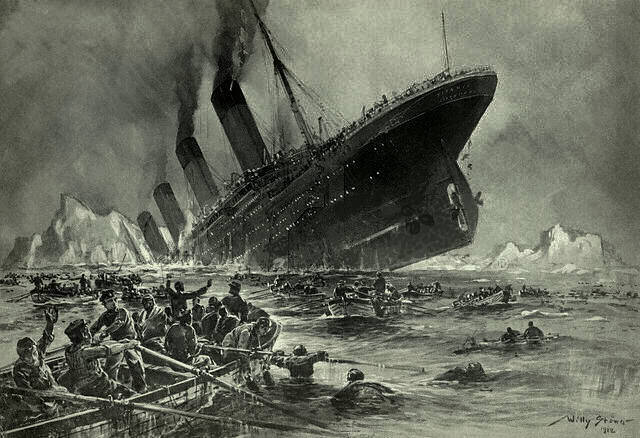
\includegraphics{figure/Titanic.jpg}
\caption{Titanic sinking by Willy Stöwer}
\end{figure}

Sinking of the RMS Titanic is one of the deadliest maritime disasters in
history (during peacetime). Over 1500 people died as a consequence of
collision with an iceberg. Projects like \emph{Encyclopedia titanica}
\texttt{https://www.encyclopedia-titanica.org/} are a source of rich and
precise data about Titanic's passengers. The data are available in a
dataset included in the \texttt{stablelearner} package. The dataset,
after some data cleaning and variable transformations, is also avaliable
in the \texttt{DALEX} package. In particular, the `titanic' data frame
contains 2207 observations (for 1317 passengers and 890 crew members)
and nine variables:

\begin{itemize}
\tightlist
\item
  \emph{gender}, person's (passenger's or crew member's) gender, a
  factor (categorical variable) with two levels (categories);
\item
  \emph{age}, person's age in years, a numerical variable; for adults,
  the age is given in (integer) years; for children younger than one
  year, the age is given as \(x/12\), where \(x\) is the number of
  months of child's age;
\item
  \emph{class}, the class in which the passenger travelled, or the duty
  class of a crew member; a factor with seven levels
\item
  \emph{embarked}, the harbor in which the person embarked on the ship,
  a factor with four levels;
\item
  \emph{country}, person's home country, a factor with 48 levels;
\item
  \emph{fare}, the price of the ticket (only available for passengers; 0
  for crew members), a numerical variable;
\item
  \emph{sibsp}, the number of siblings/spouses aboard the ship, a
  numerical variable;
\item
  \emph{parch}, the number of parents/children aboard the ship, a
  numerical variable;
\item
  \emph{survived}, a factor with two levels indicating whether the
  person survived or not.
\end{itemize}

The R code below provides more info about the contents of the dataset,
values of the variables, etc.

\begin{Shaded}
\begin{Highlighting}[]
\KeywordTok{library}\NormalTok{(}\StringTok{"DALEX"}\NormalTok{)}
\KeywordTok{head}\NormalTok{(titanic, }\DecValTok{2}\NormalTok{)}
\end{Highlighting}
\end{Shaded}

\begin{verbatim}
##   gender age class    embarked       country  fare sibsp parch survived
## 1   male  42   3rd Southampton United States  7.11     0     0       no
## 2   male  13   3rd Southampton United States 20.05     0     2       no
\end{verbatim}

\begin{Shaded}
\begin{Highlighting}[]
\KeywordTok{str}\NormalTok{(titanic)}
\end{Highlighting}
\end{Shaded}

\begin{verbatim}
## 'data.frame':    2207 obs. of  9 variables:
##  $ gender  : Factor w/ 2 levels "female","male": 2 2 2 1 1 2 2 1 2 2 ...
##  $ age     : num  42 13 16 39 16 25 30 28 27 20 ...
##  $ class   : Factor w/ 7 levels "1st","2nd","3rd",..: 3 3 3 3 3 3 2 2 3 3 ...
##  $ embarked: Factor w/ 4 levels "Belfast","Cherbourg",..: 4 4 4 4 4 4 2 2 2 4 ...
##  $ country : Factor w/ 48 levels "Argentina","Australia",..: 44 44 44 15 30 44 17 17 26 16 ...
##  $ fare    : num  7.11 20.05 20.05 20.05 7.13 ...
##  $ sibsp   : num  0 0 1 1 0 0 1 1 0 0 ...
##  $ parch   : num  0 2 1 1 0 0 0 0 0 0 ...
##  $ survived: Factor w/ 2 levels "no","yes": 1 1 1 2 2 2 1 2 2 2 ...
\end{verbatim}

\begin{Shaded}
\begin{Highlighting}[]
\KeywordTok{levels}\NormalTok{(titanic}\OperatorTok{$}\NormalTok{class)}
\end{Highlighting}
\end{Shaded}

\begin{verbatim}
## [1] "1st"              "2nd"              "3rd"             
## [4] "deck crew"        "engineering crew" "restaurant staff"
## [7] "victualling crew"
\end{verbatim}

\begin{Shaded}
\begin{Highlighting}[]
\KeywordTok{levels}\NormalTok{(titanic}\OperatorTok{$}\NormalTok{embarked)}
\end{Highlighting}
\end{Shaded}

\begin{verbatim}
## [1] "Belfast"     "Cherbourg"   "Queenstown"  "Southampton"
\end{verbatim}

Models considered for this dataset will use \emph{survived} as the
(binary) dependent variable.

\hypertarget{exploration-titanic}{%
\subsubsection{Data exploration}\label{exploration-titanic}}

It is always advisable to explore data before modelling. However, as
this book is focused on model exploration, we will limit the data
exploration part.

Before exploring the data, we first do some pre-processing. In
particular, the value of variables \emph{age}, \emph{country},
\emph{sibsp}, \emph{parch}, and \emph{fare} is missing for a limited
number of observations (2, 81, 10, 10, and 26, respectively). Analyzing
data with missing values is a topic on its own (Little and Rubin 1987;
Schafer 1997; Molenberghs and Kenward 2007). An often-used approach is
to impute the missing values. Toward this end, multiple imputation
should be considered (Schafer 1997; Molenberghs and Kenward 2007; van
Buuren 2012). However, given the limited number of missing values and
the intended illustrative use of the dataset, we will limit ourselves
to, admittedly inferior, single imputation. In particular, we replace
the missing \emph{age} values by the mean of the observed ones, i.e.,
30. Missing \emph{country} will be coded by ``X''. For \emph{sibsp} and
\emph{parch}, we replace the missing values by the most frequently
observed value, i.e., 0. Finally, for \emph{fare}, we use the mean fare
for a given \emph{class}, i.e., 0 pounds for crew, 89 pounds for the
1st, 22 pounds for the 2nd, and 13 pounds for the 3rd class. The R code
presented below implements the imputation steps.

\begin{Shaded}
\begin{Highlighting}[]
\CommentTok{# missing age is replaced by average (30)}
\NormalTok{titanic}\OperatorTok{$}\NormalTok{age[}\KeywordTok{is.na}\NormalTok{(titanic}\OperatorTok{$}\NormalTok{age)] =}\StringTok{ }\DecValTok{30}
\CommentTok{# missing country is replaced by "X"}
\NormalTok{titanic}\OperatorTok{$}\NormalTok{country <-}\StringTok{ }\KeywordTok{as.character}\NormalTok{(titanic}\OperatorTok{$}\NormalTok{country)}
\NormalTok{titanic}\OperatorTok{$}\NormalTok{country[}\KeywordTok{is.na}\NormalTok{(titanic}\OperatorTok{$}\NormalTok{country)] =}\StringTok{ "X"}
\NormalTok{titanic}\OperatorTok{$}\NormalTok{country <-}\StringTok{ }\KeywordTok{factor}\NormalTok{(titanic}\OperatorTok{$}\NormalTok{country)}
\CommentTok{# missing fare is replaced by class average}
\NormalTok{titanic}\OperatorTok{$}\NormalTok{fare[}\KeywordTok{is.na}\NormalTok{(titanic}\OperatorTok{$}\NormalTok{fare) }\OperatorTok{&}\StringTok{ }\NormalTok{titanic}\OperatorTok{$}\NormalTok{class }\OperatorTok{==}\StringTok{ "1st"}\NormalTok{] =}\StringTok{ }\DecValTok{89}
\NormalTok{titanic}\OperatorTok{$}\NormalTok{fare[}\KeywordTok{is.na}\NormalTok{(titanic}\OperatorTok{$}\NormalTok{fare) }\OperatorTok{&}\StringTok{ }\NormalTok{titanic}\OperatorTok{$}\NormalTok{class }\OperatorTok{==}\StringTok{ "2nd"}\NormalTok{] =}\StringTok{ }\DecValTok{22}
\NormalTok{titanic}\OperatorTok{$}\NormalTok{fare[}\KeywordTok{is.na}\NormalTok{(titanic}\OperatorTok{$}\NormalTok{fare) }\OperatorTok{&}\StringTok{ }\NormalTok{titanic}\OperatorTok{$}\NormalTok{class }\OperatorTok{==}\StringTok{ "3rd"}\NormalTok{] =}\StringTok{ }\DecValTok{13}
\CommentTok{# missing sibsp, parch are replaced by 0}
\NormalTok{titanic}\OperatorTok{$}\NormalTok{sibsp[}\KeywordTok{is.na}\NormalTok{(titanic}\OperatorTok{$}\NormalTok{sibsp)] =}\StringTok{ }\DecValTok{0}
\NormalTok{titanic}\OperatorTok{$}\NormalTok{parch[}\KeywordTok{is.na}\NormalTok{(titanic}\OperatorTok{$}\NormalTok{parch)] =}\StringTok{ }\DecValTok{0}
\end{Highlighting}
\end{Shaded}

After imputing the missing values, we investigate the association
between survival status and other variables. Figures
\ref{fig:titanicExplorationGender}-\ref{fig:titanicExplorationFare}
present graphically the proportion non- and survivors for different
levels of the other variables. The height of the bars (on the y-axis)
reflects the marginal distribution (proportions) of the observed levels
of the variable. On the other hand, the width of the bars (on the
x-axis) provides the information about the proportion of non- and
survivors. Note that, to construct the graphs for \emph{age} and
\emph{fare}, we categorized the range of the observed values.

Figures \ref{fig:titanicExplorationGender} and
\ref{fig:titanicExplorationAge} indicate that the proportion of
survivors was larger for females and children below 5 years of age. This
is most likely the result of the ``women and children first'' principle
that is often evoked in situations that require evacuation of persons
whose life is in danger. The principle can, perhaps, partially explain
the trend seen in Figures \ref{fig:titanicExplorationParch} and
\ref{fig:titanicExplorationSibsp}, i.e., a higher proportion of
survivors among those with 1-3 parents/children and 1-2 siblings/spouses
aboard. Figure \ref{fig:titanicExplorationClass} indicates that
passengers travelling in the first and second class had a higher chance
of survival, perhaps due to the proximity of the location of their
cabins to the deck. Interestingly, the proportion of survivors among
crew deck was similar to the proportion of the first-class passengers.
Figure \ref{fig:titanicExplorationFare} shows that the proportion of
survivors increased with the fare, which is consistent with the fact
that the proportion was higher for passengers travelling in the first
and second class. Finally, Figures \ref{fig:titanicExplorationEmbarked}
and \ref{fig:titanicExplorationCountry} do not suggest any noteworthy
trends.

\begin{figure}

{\centering 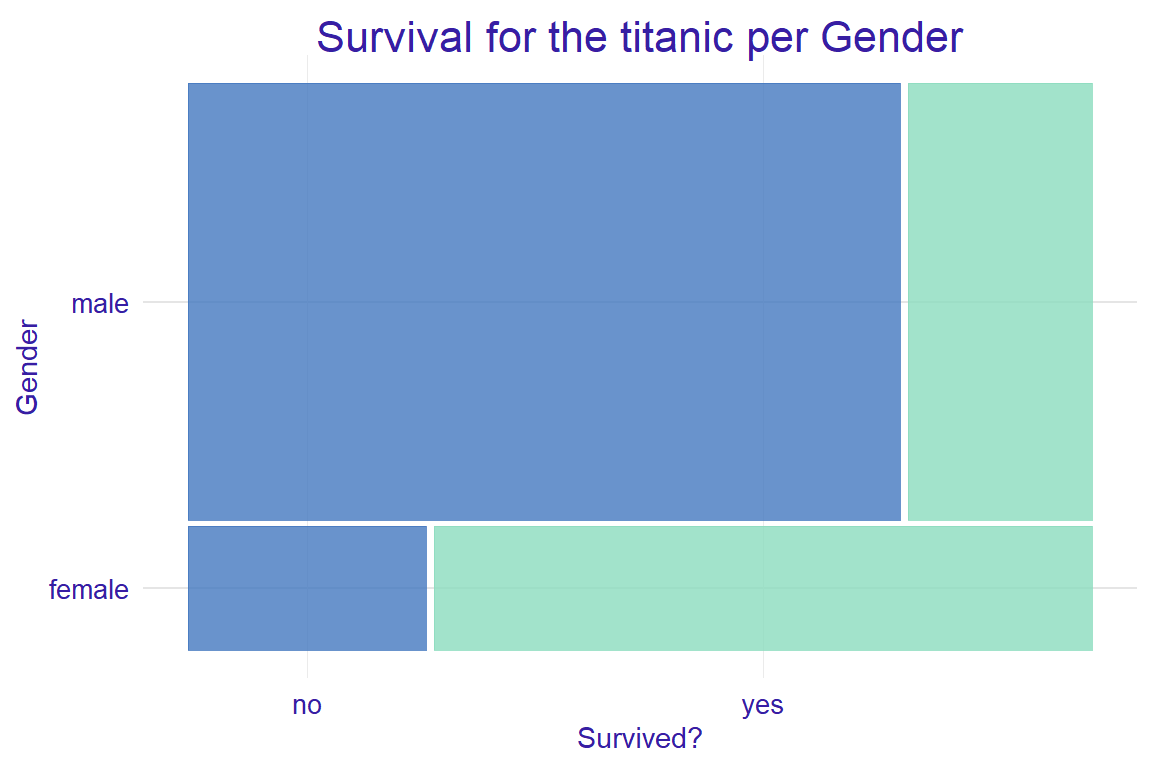
\includegraphics[width=0.7\linewidth]{PM_VEE_files/figure-latex/titanicExplorationGender-1} 

}

\caption{Survival according to gender in the Titanic data.}\label{fig:titanicExplorationGender}
\end{figure}

\begin{figure}

{\centering 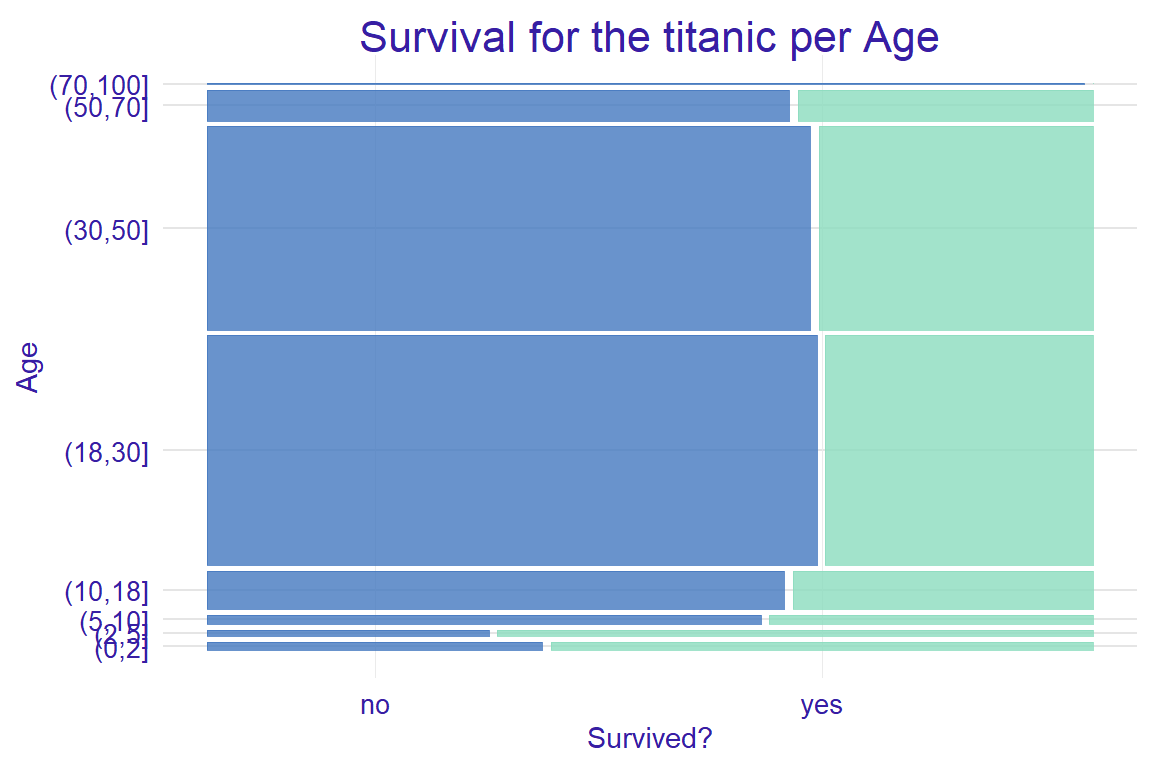
\includegraphics[width=0.7\linewidth]{PM_VEE_files/figure-latex/titanicExplorationAge-1} 

}

\caption{Survival accroding to age group in the Titanic data.}\label{fig:titanicExplorationAge}
\end{figure}

\begin{figure}

{\centering 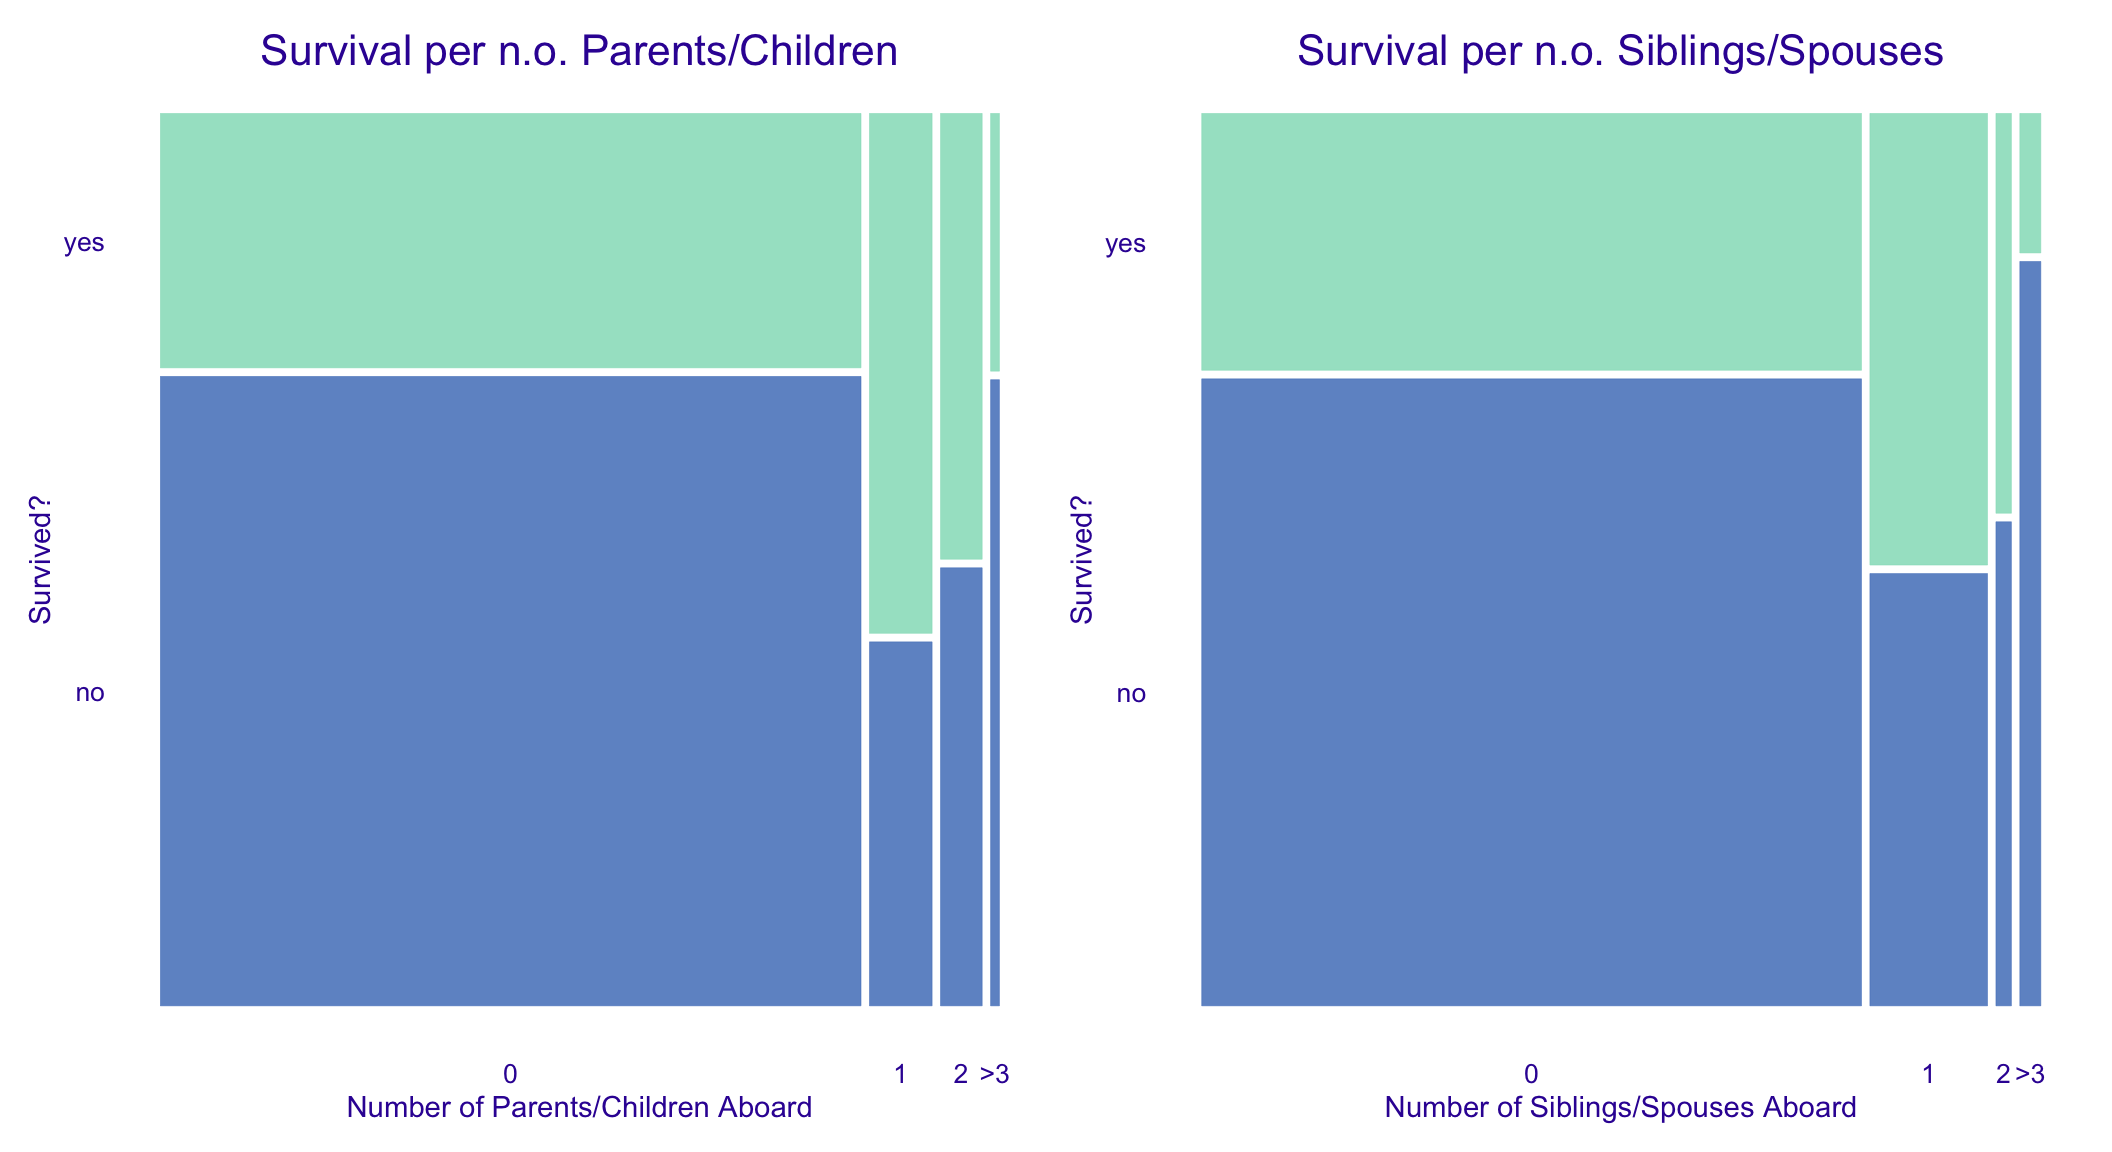
\includegraphics[width=0.7\linewidth]{PM_VEE_files/figure-latex/titanicExplorationParch-1} 

}

\caption{Survival according to the number of parents/children in the Titanic data.}\label{fig:titanicExplorationParch}
\end{figure}

\begin{figure}

{\centering 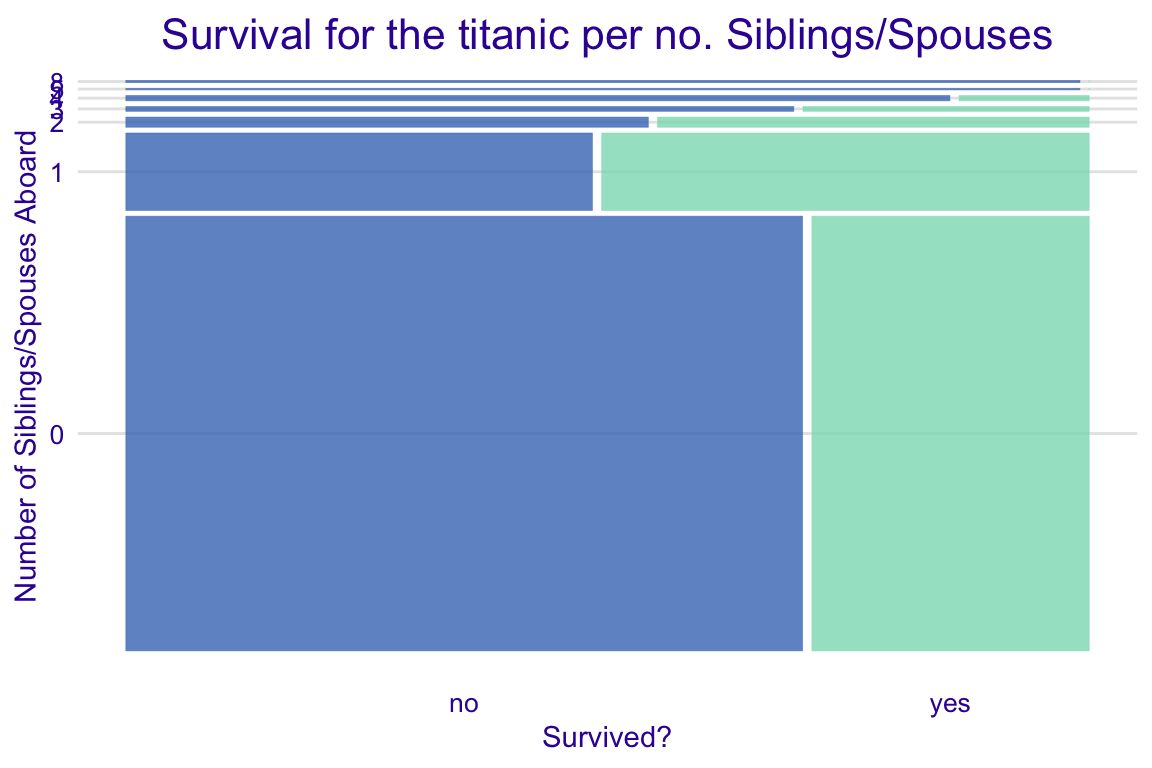
\includegraphics[width=0.7\linewidth]{PM_VEE_files/figure-latex/titanicExplorationSibsp-1} 

}

\caption{Survival according to the number of siblings/spouses in the Titanic data.}\label{fig:titanicExplorationSibsp}
\end{figure}
\begin{figure}

{\centering 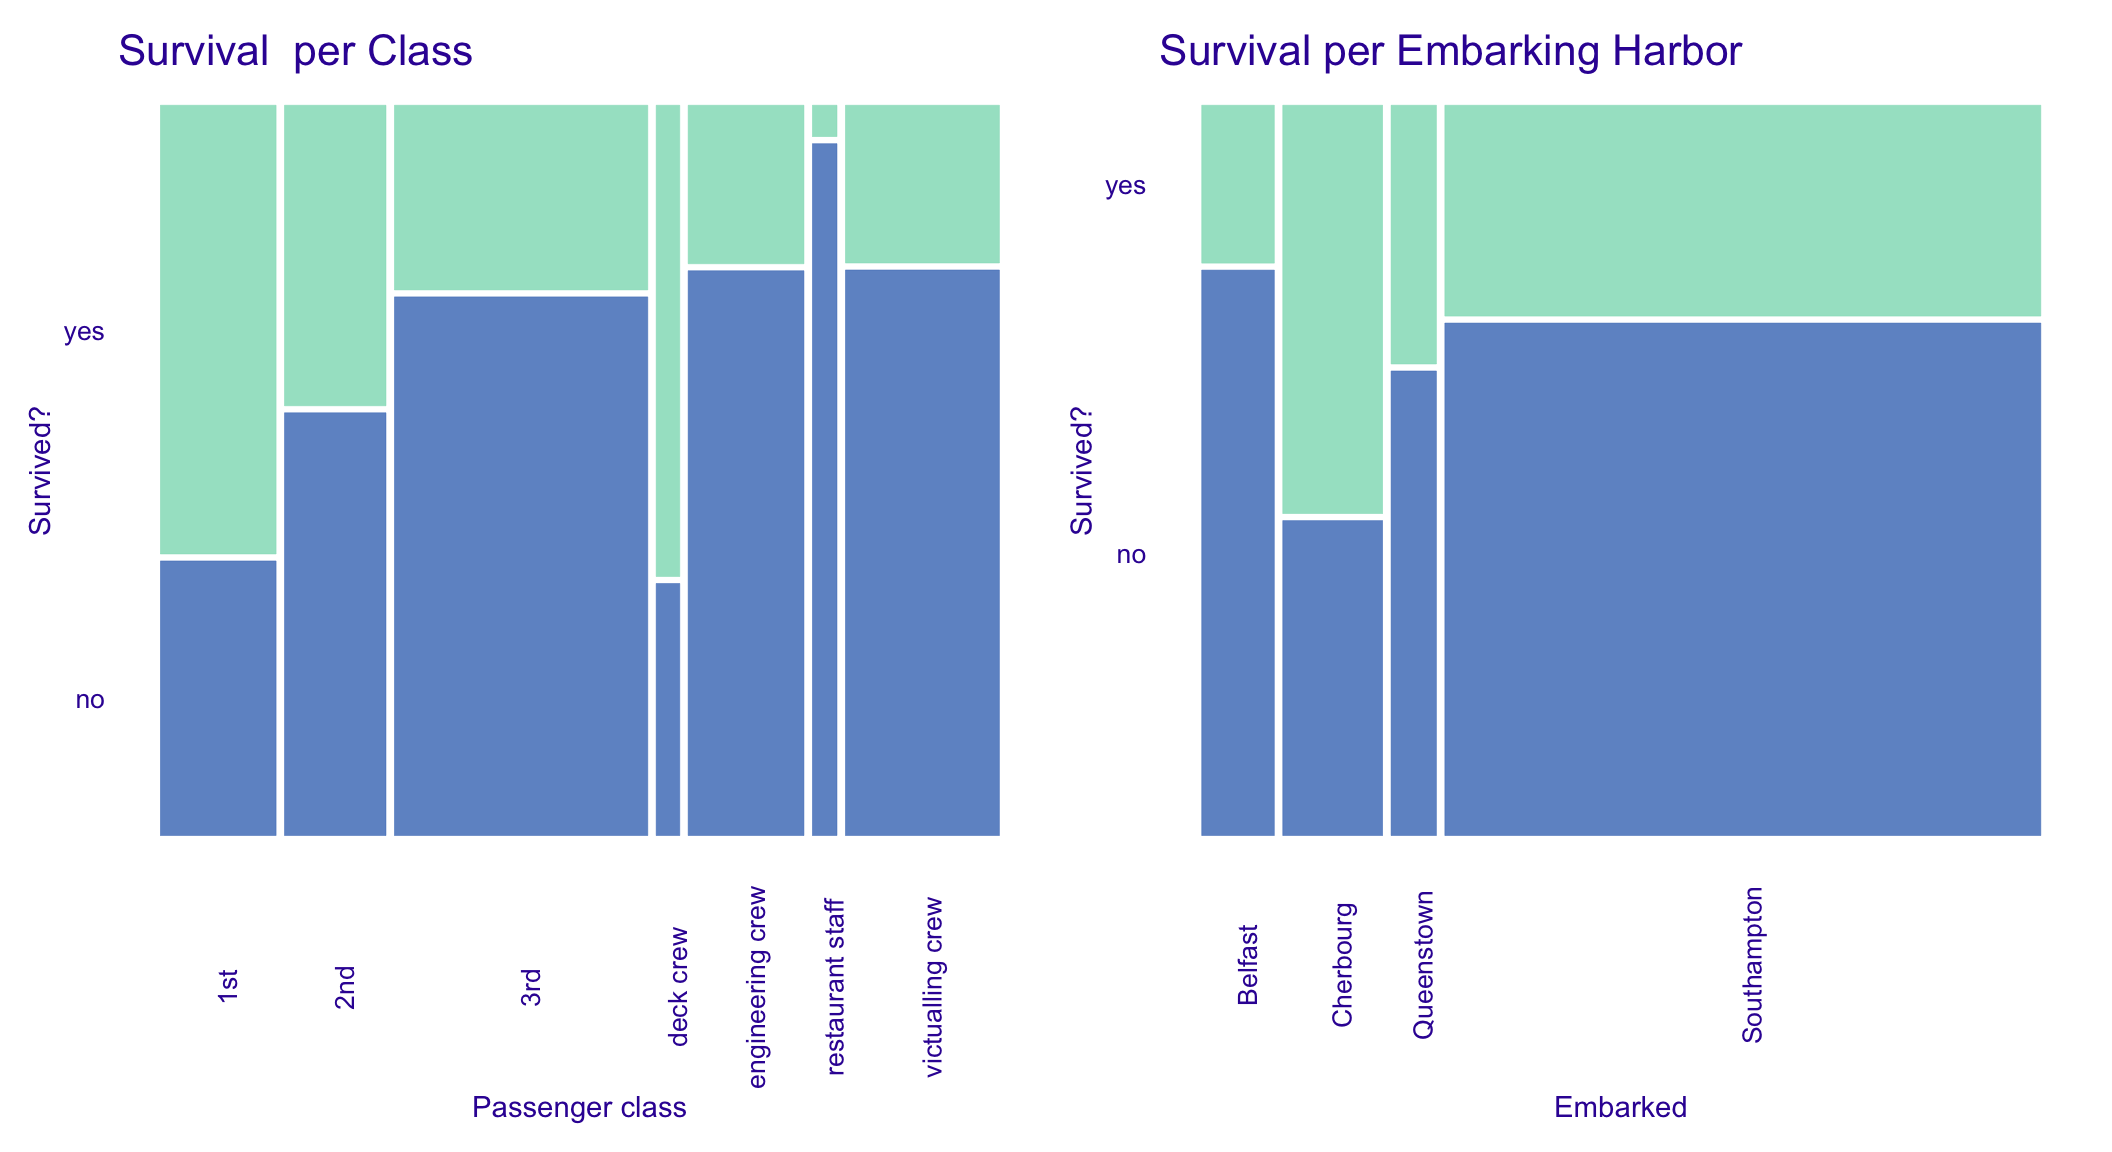
\includegraphics[width=0.7\linewidth]{PM_VEE_files/figure-latex/titanicExplorationClass-1} 

}

\caption{Survival according to the class in the Titanic data.}\label{fig:titanicExplorationClass}
\end{figure}

\begin{figure}

{\centering 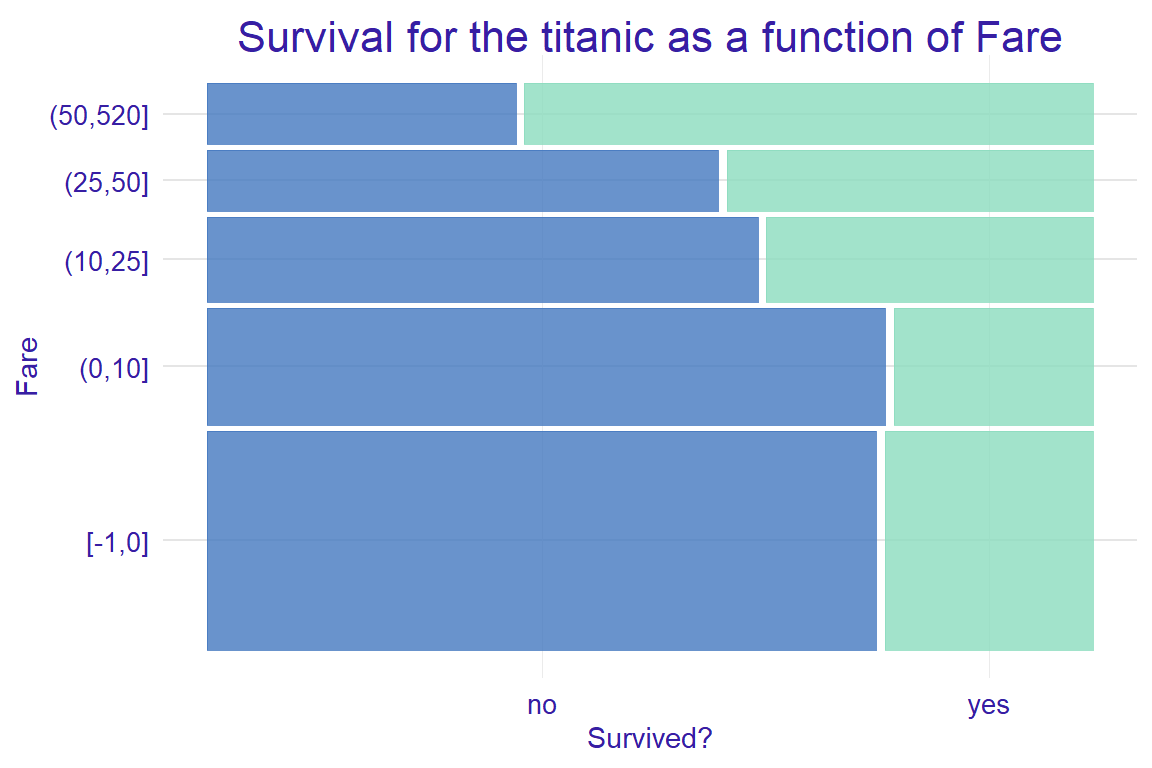
\includegraphics[width=0.7\linewidth]{PM_VEE_files/figure-latex/titanicExplorationFare-1} 

}

\caption{Survival according to fare in the Titanic data.}\label{fig:titanicExplorationFare}
\end{figure}

\begin{figure}

{\centering 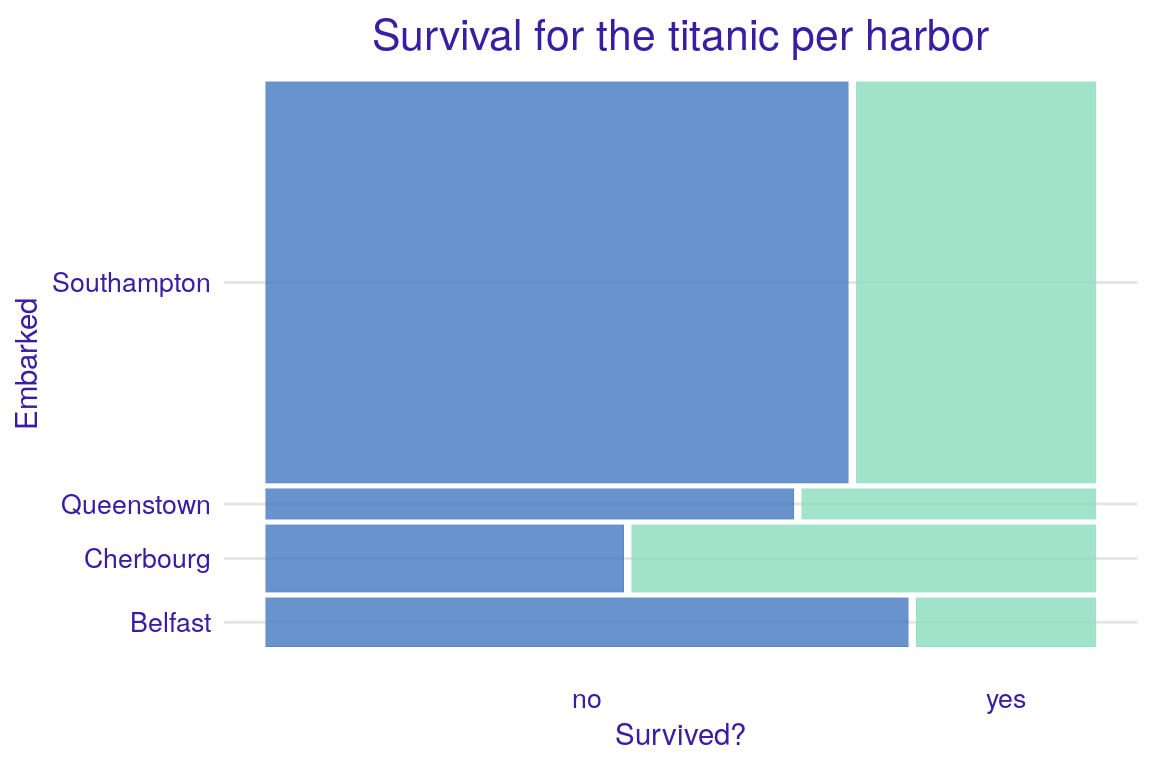
\includegraphics[width=0.7\linewidth]{PM_VEE_files/figure-latex/titanicExplorationEmbarked-1} 

}

\caption{Survival according to the port of embarking in the Titanic data.}\label{fig:titanicExplorationEmbarked}
\end{figure}

\begin{figure}

{\centering 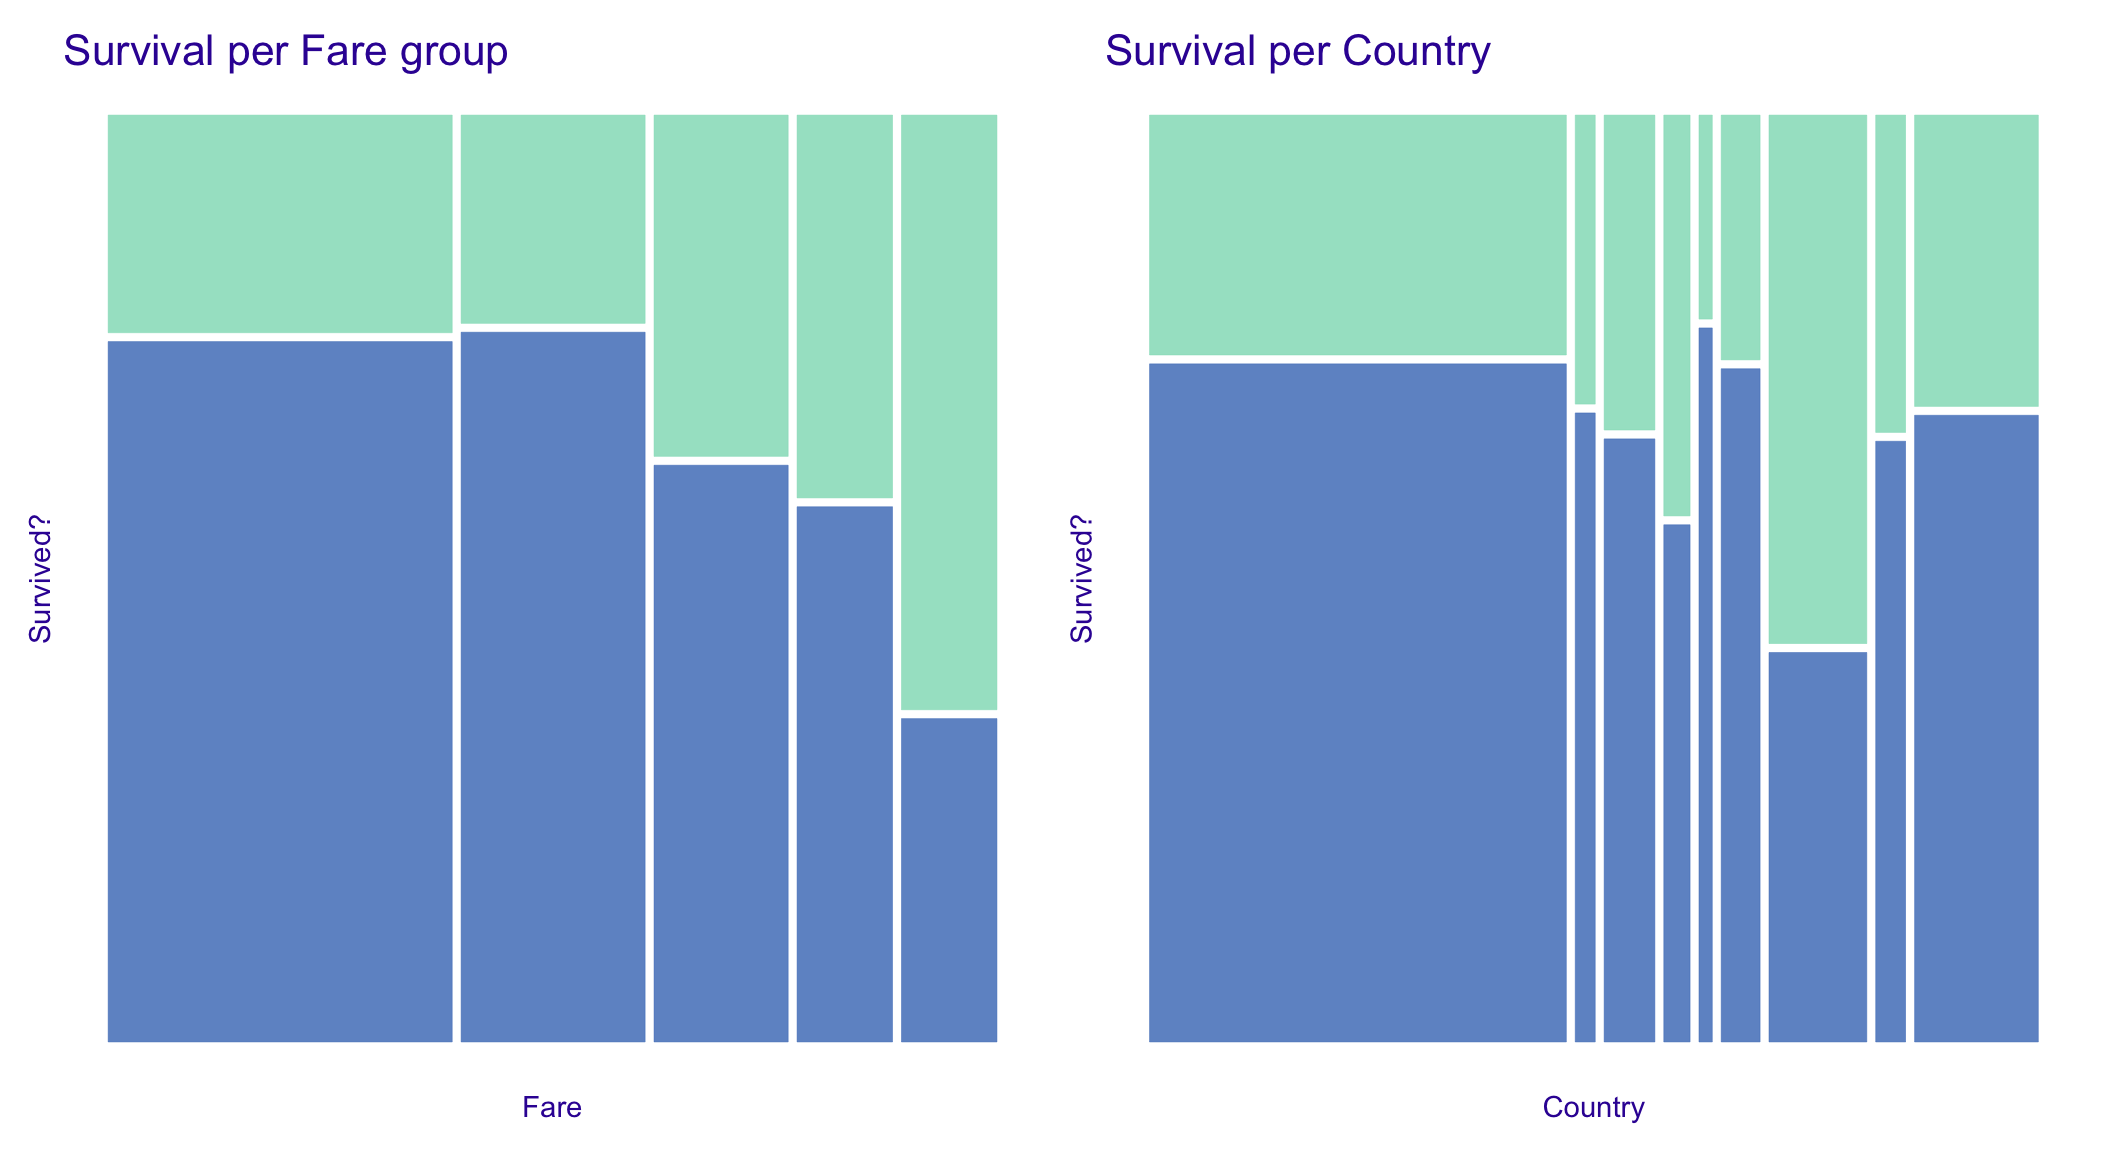
\includegraphics[width=0.7\linewidth]{PM_VEE_files/figure-latex/titanicExplorationCountry-1} 

}

\caption{Survival according to country in the Titanic data.}\label{fig:titanicExplorationCountry}
\end{figure}

\hypertarget{model-titanic-lmr}{%
\subsubsection{Logistic regression}\label{model-titanic-lmr}}

The dependent variable of interest, \emph{survival}, is binary. Thus, a
natural choice to build a predictive model is logistic regression. We do
not consider country as an explanatory variable. As there is no reason
to expect a linear relationship between age and odds of survival, we use
linear tail-restricted cubic splines, available in the \texttt{rcs()}
function of the \texttt{rms} package \citep{rms}, to model the effect of
age. We also do not expect linear relation for the \texttt{fare}
variable, but because of it's skewness, we do not use splines for this
variable. The results of the model are stored in model-object
\texttt{titanic\_lmr\_v6}, which will be used in subsequent chapters.

\begin{Shaded}
\begin{Highlighting}[]
\KeywordTok{library}\NormalTok{(}\StringTok{"rms"}\NormalTok{)}
\KeywordTok{set.seed}\NormalTok{(}\DecValTok{1313}\NormalTok{)}
\NormalTok{titanic_lmr_v6 <-}\StringTok{ }\KeywordTok{lrm}\NormalTok{(survived }\OperatorTok{==}\StringTok{ "yes"} \OperatorTok{~}\StringTok{ }\NormalTok{gender }\OperatorTok{+}\StringTok{ }\KeywordTok{rcs}\NormalTok{(age) }\OperatorTok{+}\StringTok{ }\NormalTok{class }\OperatorTok{+}\StringTok{ }\NormalTok{sibsp }\OperatorTok{+}
\StringTok{                   }\NormalTok{parch }\OperatorTok{+}\StringTok{ }\NormalTok{fare }\OperatorTok{+}\StringTok{ }\NormalTok{embarked, titanic)}
\NormalTok{titanic_lmr_v6}
\end{Highlighting}
\end{Shaded}

\begin{verbatim}
## Logistic Regression Model
##  
##  lrm(formula = survived == "yes" ~ gender + rcs(age) + class + 
##      sibsp + parch + fare + embarked, data = titanic)
##  
##                         Model Likelihood     Discrimination    Rank Discrim.    
##                            Ratio Test           Indexes           Indexes       
##  Obs           2207    LR chi2     752.06    R2       0.404    C       0.817    
##   FALSE        1496    d.f.            17    g        1.647    Dxy     0.635    
##   TRUE          711    Pr(> chi2) <0.0001    gr       5.191    gamma   0.636    
##  max |deriv| 0.0001                          gp       0.282    tau-a   0.277    
##                                              Brier    0.146                     
##  
##                         Coef    S.E.   Wald Z Pr(>|Z|)
##  Intercept               4.5746 0.5480   8.35 <0.0001 
##  gender=male            -2.7687 0.1586 -17.45 <0.0001 
##  age                    -0.1180 0.0221  -5.35 <0.0001 
##  age'                    0.6313 0.1628   3.88 0.0001  
##  age''                  -2.6583 0.7840  -3.39 0.0007  
##  age'''                  2.8977 1.0130   2.86 0.0042  
##  class=2nd              -1.1390 0.2501  -4.56 <0.0001 
##  class=3rd              -2.0627 0.2490  -8.28 <0.0001 
##  class=deck crew         1.0672 0.3498   3.05 0.0023  
##  class=engineering crew -0.9702 0.2648  -3.66 0.0002  
##  class=restaurant staff -3.1712 0.6583  -4.82 <0.0001 
##  class=victualling crew -1.0877 0.2596  -4.19 <0.0001 
##  sibsp                  -0.4504 0.1006  -4.48 <0.0001 
##  parch                  -0.0871 0.0987  -0.88 0.3776  
##  fare                    0.0014 0.0020   0.70 0.4842  
##  embarked=Cherbourg      0.7881 0.2836   2.78 0.0055  
##  embarked=Queenstown     0.2745 0.3409   0.80 0.4208  
##  embarked=Southampton    0.2343 0.2119   1.11 0.2689  
## 
\end{verbatim}

\hypertarget{model-titanic-rf}{%
\subsubsection{Random forest}\label{model-titanic-rf}}

As an alternative to a logistic regression model, we consider a random
forest model. Random forest is known for good predictive performance, is
able to grasp low-level variable interactions, and is quite stable
\citep{randomForestBreiman}. To fit the model, we apply the
\texttt{randomForest()} function, with default settings, from the
package with the same name \citep{randomForestRNews}.

In the first instance, we fit a model with the same set of explanatory
variables as the logistic regression model. The results of the model are
stored in model-object \texttt{titanic\_rf\_v6}.

\begin{Shaded}
\begin{Highlighting}[]
\KeywordTok{library}\NormalTok{(}\StringTok{"randomForest"}\NormalTok{)}
\KeywordTok{set.seed}\NormalTok{(}\DecValTok{1313}\NormalTok{)}
\NormalTok{titanic_rf_v6 <-}\StringTok{ }\KeywordTok{randomForest}\NormalTok{(survived }\OperatorTok{~}\StringTok{ }\NormalTok{class }\OperatorTok{+}\StringTok{ }\NormalTok{gender }\OperatorTok{+}\StringTok{ }\NormalTok{age }\OperatorTok{+}\StringTok{ }\NormalTok{sibsp }\OperatorTok{+}\StringTok{ }\NormalTok{parch }\OperatorTok{+}\StringTok{ }\NormalTok{fare }\OperatorTok{+}\StringTok{ }\NormalTok{embarked, }
                           \DataTypeTok{data =}\NormalTok{ titanic)}
\NormalTok{titanic_rf_v6}
\end{Highlighting}
\end{Shaded}

\begin{verbatim}
## 
## Call:
##  randomForest(formula = survived ~ class + gender + age + sibsp +      parch + fare + embarked, data = titanic) 
##                Type of random forest: classification
##                      Number of trees: 500
## No. of variables tried at each split: 2
## 
##         OOB estimate of  error rate: 18.62%
## Confusion matrix:
##       no yes class.error
## no  1393 103  0.06885027
## yes  308 403  0.43319269
\end{verbatim}

For comparison purposes, we also consider a model with only three
explanatory variables: \emph{class}, \emph{gender}, and \emph{age}. The
results of the model are stored in model-object
\texttt{titanic\_rf\_v3}.

\begin{Shaded}
\begin{Highlighting}[]
\NormalTok{titanic_rf_v3 <-}\StringTok{ }\KeywordTok{randomForest}\NormalTok{(survived }\OperatorTok{~}\StringTok{ }\NormalTok{class }\OperatorTok{+}\StringTok{ }\NormalTok{gender }\OperatorTok{+}\StringTok{ }\NormalTok{age, }\DataTypeTok{data =}\NormalTok{ titanic)}
\NormalTok{titanic_rf_v3}
\end{Highlighting}
\end{Shaded}

\begin{verbatim}
## 
## Call:
##  randomForest(formula = survived ~ class + gender + age, data = titanic) 
##                Type of random forest: classification
##                      Number of trees: 500
## No. of variables tried at each split: 1
## 
##         OOB estimate of  error rate: 21.02%
## Confusion matrix:
##       no yes class.error
## no  1367 129  0.08622995
## yes  335 376  0.47116737
\end{verbatim}

\hypertarget{model-titanic-gbm}{%
\subsubsection{Gradient boosting}\label{model-titanic-gbm}}

Finally, we consider the gradient-boosting model.
\citep{Friedman00greedyfunction} The model is known for being able to
accomodate higher-order interactions between variables. We use the same
set of explanatory variables as for the logistic regression model. To
fit the gradient-boosting model, we use function \texttt{gbm()} from the
\texttt{gbm} package \citep{gbm}. The results of the model are stored in
model-object \texttt{titanic\_gbm\_v6}.

\begin{Shaded}
\begin{Highlighting}[]
\KeywordTok{library}\NormalTok{(}\StringTok{"gbm"}\NormalTok{)}
\KeywordTok{set.seed}\NormalTok{(}\DecValTok{1313}\NormalTok{)}
\NormalTok{titanic_gbm_v6 <-}\StringTok{ }\KeywordTok{gbm}\NormalTok{(survived }\OperatorTok{==}\StringTok{ "yes"} \OperatorTok{~}\StringTok{ }\NormalTok{class }\OperatorTok{+}\StringTok{ }\NormalTok{gender }\OperatorTok{+}\StringTok{ }\NormalTok{age }\OperatorTok{+}\StringTok{ }\NormalTok{sibsp }\OperatorTok{+}\StringTok{ }\NormalTok{parch }\OperatorTok{+}\StringTok{ }\NormalTok{fare }\OperatorTok{+}\StringTok{ }\NormalTok{embarked, }
                      \DataTypeTok{data =}\NormalTok{ titanic, }\DataTypeTok{n.trees =} \DecValTok{15000}\NormalTok{)}
\end{Highlighting}
\end{Shaded}

\begin{verbatim}
## Distribution not specified, assuming bernoulli ...
\end{verbatim}

\begin{Shaded}
\begin{Highlighting}[]
\NormalTok{titanic_gbm_v6}
\end{Highlighting}
\end{Shaded}

\begin{verbatim}
## gbm(formula = survived == "yes" ~ class + gender + age + sibsp + 
##     parch + fare + embarked, data = titanic, n.trees = 15000)
## A gradient boosted model with bernoulli loss function.
## 15000 iterations were performed.
## There were 7 predictors of which 7 had non-zero influence.
\end{verbatim}

\hypertarget{predictions-titanic}{%
\subsubsection{Model predictions}\label{predictions-titanic}}

Let us now compare predictions that are obtained from the three
different models. In particular, we will compute the predicted
probability of survival for an 8-year-old boy who embarked in Belfast
and travelled in the 1-st class with no parents nor siblings and with a
ticket costing 72 pounds.

First, we create a data frame \texttt{johny\_d} that contains the data
describing the passenger.

\begin{Shaded}
\begin{Highlighting}[]
\NormalTok{johny_d <-}\StringTok{ }\KeywordTok{data.frame}\NormalTok{(}
            \DataTypeTok{class =} \KeywordTok{factor}\NormalTok{(}\StringTok{"1st"}\NormalTok{, }\DataTypeTok{levels =} \KeywordTok{c}\NormalTok{(}\StringTok{"1st"}\NormalTok{, }\StringTok{"2nd"}\NormalTok{, }\StringTok{"3rd"}\NormalTok{, }\StringTok{"deck crew"}\NormalTok{, }\StringTok{"engineering crew"}\NormalTok{, }\StringTok{"restaurant staff"}\NormalTok{, }\StringTok{"victualling crew"}\NormalTok{)),}
            \DataTypeTok{gender =} \KeywordTok{factor}\NormalTok{(}\StringTok{"male"}\NormalTok{, }\DataTypeTok{levels =} \KeywordTok{c}\NormalTok{(}\StringTok{"female"}\NormalTok{, }\StringTok{"male"}\NormalTok{)),}
            \DataTypeTok{age =} \DecValTok{8}\NormalTok{,}
            \DataTypeTok{sibsp =} \DecValTok{0}\NormalTok{,}
            \DataTypeTok{parch =} \DecValTok{0}\NormalTok{,}
            \DataTypeTok{fare =} \DecValTok{72}\NormalTok{,}
            \DataTypeTok{embarked =} \KeywordTok{factor}\NormalTok{(}\StringTok{"Belfast"}\NormalTok{, }\DataTypeTok{levels =} \KeywordTok{c}\NormalTok{(}\StringTok{"Belfast"}\NormalTok{,}\StringTok{"Cherbourg"}\NormalTok{,}\StringTok{"Queenstown"}\NormalTok{,}\StringTok{"Southampton"}\NormalTok{))}
\NormalTok{)}
\end{Highlighting}
\end{Shaded}

Subsequently, we use the generic function \texttt{predict()} to get the
predicted probability of survival for the logistic regression model.

\begin{Shaded}
\begin{Highlighting}[]
\NormalTok{(pred_lmr <-}\StringTok{ }\KeywordTok{predict}\NormalTok{(titanic_lmr_v6, johny_d, }\DataTypeTok{type =} \StringTok{"fitted"}\NormalTok{))}
\end{Highlighting}
\end{Shaded}

\begin{verbatim}
##         1 
## 0.7233413
\end{verbatim}

The predicted probability is equal to 0.72.

We do the same for the random forest and gradient boosting models.

\begin{Shaded}
\begin{Highlighting}[]
\NormalTok{(pred_rf <-}\StringTok{ }\KeywordTok{predict}\NormalTok{(titanic_rf_v6, johny_d, }\DataTypeTok{type =} \StringTok{"prob"}\NormalTok{))}
\end{Highlighting}
\end{Shaded}

\begin{verbatim}
##      no   yes
## 1 0.626 0.374
## attr(,"class")
## [1] "matrix" "votes"
\end{verbatim}

\begin{Shaded}
\begin{Highlighting}[]
\NormalTok{(pred_gbm <-}\StringTok{ }\KeywordTok{predict}\NormalTok{(titanic_gbm_v6, johny_d, }\DataTypeTok{type =} \StringTok{"response"}\NormalTok{, }\DataTypeTok{n.trees =} \DecValTok{15000}\NormalTok{))}
\end{Highlighting}
\end{Shaded}

\begin{verbatim}
## [1] 0.6700909
\end{verbatim}

As a result, we obtain the predicted probabilities of 0.37 and 0.67,
respectively.

The models lead to different probabilities. Thus, it might be of
interest to understand the reason for the differences, as it could help
us to decide which of the predictions we might want to trust.

Note that for some examples we will use another observation (instance)
with lower chances of survival. Let's call this passenger Henry.

\begin{Shaded}
\begin{Highlighting}[]
\NormalTok{henry <-}\StringTok{ }\KeywordTok{data.frame}\NormalTok{(}
            \DataTypeTok{class =} \KeywordTok{factor}\NormalTok{(}\StringTok{"1st"}\NormalTok{, }\DataTypeTok{levels =} \KeywordTok{c}\NormalTok{(}\StringTok{"1st"}\NormalTok{, }\StringTok{"2nd"}\NormalTok{, }\StringTok{"3rd"}\NormalTok{, }\StringTok{"deck crew"}\NormalTok{, }\StringTok{"engineering crew"}\NormalTok{, }\StringTok{"restaurant staff"}\NormalTok{, }\StringTok{"victualling crew"}\NormalTok{)),}
            \DataTypeTok{gender =} \KeywordTok{factor}\NormalTok{(}\StringTok{"male"}\NormalTok{, }\DataTypeTok{levels =} \KeywordTok{c}\NormalTok{(}\StringTok{"female"}\NormalTok{, }\StringTok{"male"}\NormalTok{)),}
            \DataTypeTok{age =} \DecValTok{47}\NormalTok{,}
            \DataTypeTok{sibsp =} \DecValTok{0}\NormalTok{,}
            \DataTypeTok{parch =} \DecValTok{0}\NormalTok{,}
            \DataTypeTok{fare =} \DecValTok{25}\NormalTok{,}
            \DataTypeTok{embarked =} \KeywordTok{factor}\NormalTok{(}\StringTok{"Cherbourg"}\NormalTok{, }\DataTypeTok{levels =} \KeywordTok{c}\NormalTok{(}\StringTok{"Belfast"}\NormalTok{,}\StringTok{"Cherbourg"}\NormalTok{,}\StringTok{"Queenstown"}\NormalTok{,}\StringTok{"Southampton"}\NormalTok{))}
\NormalTok{)}
\KeywordTok{round}\NormalTok{(}\KeywordTok{predict}\NormalTok{(titanic_lmr_v6, henry, }\DataTypeTok{type =} \StringTok{"fitted"}\NormalTok{),}\DecValTok{2}\NormalTok{)}
\end{Highlighting}
\end{Shaded}

\begin{verbatim}
##    1 
## 0.43
\end{verbatim}

\begin{Shaded}
\begin{Highlighting}[]
\KeywordTok{round}\NormalTok{(}\KeywordTok{predict}\NormalTok{(titanic_rf_v6, henry, }\DataTypeTok{type =} \StringTok{"prob"}\NormalTok{)[}\DecValTok{1}\NormalTok{,}\DecValTok{2}\NormalTok{],}\DecValTok{2}\NormalTok{)}
\end{Highlighting}
\end{Shaded}

\begin{verbatim}
## [1] 0.25
\end{verbatim}

\begin{Shaded}
\begin{Highlighting}[]
\KeywordTok{round}\NormalTok{(}\KeywordTok{predict}\NormalTok{(titanic_gbm_v6, henry, }\DataTypeTok{type =} \StringTok{"response"}\NormalTok{, }\DataTypeTok{n.trees =} \DecValTok{15000}\NormalTok{),}\DecValTok{2}\NormalTok{)}
\end{Highlighting}
\end{Shaded}

\begin{verbatim}
## [1] 0.42
\end{verbatim}

\hypertarget{ExplainersTitanicRCode}{%
\subsubsection{Explainers}\label{ExplainersTitanicRCode}}

Model-objects created with different libraries may have different
internal structures. Thus, first, we have got to create a wrapper around
the model. Toward this end, we use the \texttt{explain()} function from
the \texttt{DALEX} package \citep{R-DALEX}. The function requires five
arguments:

\begin{itemize}
\tightlist
\item
  \texttt{model}, a model-object;
\item
  \texttt{data}, a validation data frame;
\item
  \texttt{y}, observed values of the dependent variable for the
  validation data;
\item
  \texttt{predict\_function}, a function that returns prediction scores;
  if not specified, then a default \texttt{predict()} function is used;
\item
  \texttt{label}, a function that returns prediction scores; if not
  specified, then it is extracted from the \texttt{class(model)}. In the
  example below we create explainers for the logistic regression, random
  forest, and gradient boosting models created for the Titanic data.
\end{itemize}

Each explainer wraps all elements needed to create a model explanation,
i.e., a suitable \texttt{predict()} function, validation data set, and
the model object. Thus, in subsequent chapters we will use the
explainers instead of the model objects to keep code snippets more
concise.

\begin{Shaded}
\begin{Highlighting}[]
\NormalTok{explain_titanic_lmr_v6 <-}\StringTok{ }\KeywordTok{explain}\NormalTok{(}\DataTypeTok{model =}\NormalTok{ titanic_lmr_v6, }
                                 \DataTypeTok{data =}\NormalTok{ titanic[, }\DecValTok{-9}\NormalTok{],}
                                 \DataTypeTok{y =}\NormalTok{ titanic}\OperatorTok{$}\NormalTok{survived }\OperatorTok{==}\StringTok{ "yes"}\NormalTok{, }
                                 \DataTypeTok{predict_function =} \ControlFlowTok{function}\NormalTok{(m, x) }\KeywordTok{predict}\NormalTok{(m, x, }\DataTypeTok{type =} \StringTok{"fitted"}\NormalTok{),}
                                 \DataTypeTok{label =} \StringTok{"Logistic Regression v6"}\NormalTok{)}
\NormalTok{explain_titanic_rf_v6 <-}\StringTok{ }\KeywordTok{explain}\NormalTok{(}\DataTypeTok{model =}\NormalTok{ titanic_rf_v6, }
                                 \DataTypeTok{data =}\NormalTok{ titanic[, }\DecValTok{-9}\NormalTok{],}
                                 \DataTypeTok{y =}\NormalTok{ titanic}\OperatorTok{$}\NormalTok{survived }\OperatorTok{==}\StringTok{ "yes"}\NormalTok{, }
                                 \DataTypeTok{label =} \StringTok{"Random Forest v6"}\NormalTok{)}
\NormalTok{explain_titanic_rf_v3 <-}\StringTok{ }\KeywordTok{explain}\NormalTok{(}\DataTypeTok{model =}\NormalTok{ titanic_rf_v3, }
                                 \DataTypeTok{data =}\NormalTok{ titanic[, }\DecValTok{-9}\NormalTok{],}
                                 \DataTypeTok{y =}\NormalTok{ titanic}\OperatorTok{$}\NormalTok{survived }\OperatorTok{==}\StringTok{ "yes"}\NormalTok{, }
                                 \DataTypeTok{label =} \StringTok{"Random Forest v3"}\NormalTok{)}
\NormalTok{explain_titanic_gbm_v6 <-}\StringTok{ }\KeywordTok{explain}\NormalTok{(}\DataTypeTok{model =}\NormalTok{ titanic_gbm_v6, }
                                 \DataTypeTok{data =}\NormalTok{ titanic[, }\DecValTok{-9}\NormalTok{],}
                                 \DataTypeTok{y =}\NormalTok{ titanic}\OperatorTok{$}\NormalTok{survived }\OperatorTok{==}\StringTok{ "yes"}\NormalTok{, }
                                 \DataTypeTok{label =} \StringTok{"Generalized Boosted Regression v6"}\NormalTok{)}
\end{Highlighting}
\end{Shaded}

\hypertarget{ListOfModelsTitanic}{%
\subsubsection{\texorpdfstring{List of objects for the \texttt{titanic}
example}{List of objects for the titanic example}}\label{ListOfModelsTitanic}}

In the previous sections we have built several predictive models for the
\texttt{titanic} data set. The models will be used in the rest of the
book to illustrate the model explanation methods and tools.

For the ease of reference, we summarize the models in Table
\ref{tab:archivistHooksOfModelsTitanic}. The binary model-objects can be
downloaded by using the indicated \texttt{archivist} hooks
\citep{archivist}. By calling a function specified in the last column of
the table, one can recreate a selected model in a local R environment.

\begin{longtable}[]{@{}llll@{}}
\caption{\label{tab:archivistHooksOfModelsTitanic} Predictive models created
for the \texttt{titanic} dataset.}\tabularnewline
\toprule
\begin{minipage}[b]{0.21\columnwidth}\raggedright
Model name\strut
\end{minipage} & \begin{minipage}[b]{0.25\columnwidth}\raggedright
Model generator\strut
\end{minipage} & \begin{minipage}[b]{0.18\columnwidth}\raggedright
Variables\strut
\end{minipage} & \begin{minipage}[b]{0.25\columnwidth}\raggedright
Archivist hooks\strut
\end{minipage}\tabularnewline
\midrule
\endfirsthead
\toprule
\begin{minipage}[b]{0.21\columnwidth}\raggedright
Model name\strut
\end{minipage} & \begin{minipage}[b]{0.25\columnwidth}\raggedright
Model generator\strut
\end{minipage} & \begin{minipage}[b]{0.18\columnwidth}\raggedright
Variables\strut
\end{minipage} & \begin{minipage}[b]{0.25\columnwidth}\raggedright
Archivist hooks\strut
\end{minipage}\tabularnewline
\midrule
\endhead
\begin{minipage}[t]{0.21\columnwidth}\raggedright
\texttt{titanic\_lmr\_v6}\strut
\end{minipage} & \begin{minipage}[t]{0.25\columnwidth}\raggedright
\texttt{rms::\ lmr} v.5.1.3\strut
\end{minipage} & \begin{minipage}[t]{0.18\columnwidth}\raggedright
gender, age, class, sibsp, parch, fare, embarked\strut
\end{minipage} & \begin{minipage}[t]{0.25\columnwidth}\raggedright
Get the model: \texttt{archivist::\ aread("pbiecek/models/ceb40")}. Get
the explainer: \texttt{archivist::\ aread("pbiecek/models/2b9b6")}\strut
\end{minipage}\tabularnewline
\begin{minipage}[t]{0.21\columnwidth}\raggedright
\texttt{titanic\_rf\_v6}\strut
\end{minipage} & \begin{minipage}[t]{0.25\columnwidth}\raggedright
\texttt{randomForest::\ randomForest} v.4.6.14\strut
\end{minipage} & \begin{minipage}[t]{0.18\columnwidth}\raggedright
gender, age, class, sibsp, parch, fare, embarked\strut
\end{minipage} & \begin{minipage}[t]{0.25\columnwidth}\raggedright
Get the model: \texttt{archivist::\ aread("pbiecek/models/1f938")}. Get
the explainer: \texttt{archivist::\ aread("pbiecek/models/9b971")}\strut
\end{minipage}\tabularnewline
\begin{minipage}[t]{0.21\columnwidth}\raggedright
\texttt{titanic\_rf\_v3}\strut
\end{minipage} & \begin{minipage}[t]{0.25\columnwidth}\raggedright
\texttt{randomForest::\ randomForest} v.4.6.14\strut
\end{minipage} & \begin{minipage}[t]{0.18\columnwidth}\raggedright
gender, age, class\strut
\end{minipage} & \begin{minipage}[t]{0.25\columnwidth}\raggedright
Get the model: \texttt{archivist::\ aread("pbiecek/models/855c1")}. Get
the explainer: \texttt{archivist::\ aread("pbiecek/models/92754")}\strut
\end{minipage}\tabularnewline
\begin{minipage}[t]{0.21\columnwidth}\raggedright
\texttt{titanic\_gbm\_v6}\strut
\end{minipage} & \begin{minipage}[t]{0.25\columnwidth}\raggedright
\texttt{gbm::\ gbm} v.2.1.5\strut
\end{minipage} & \begin{minipage}[t]{0.18\columnwidth}\raggedright
gender, age, class, sibsp, parch, fare, embarked\strut
\end{minipage} & \begin{minipage}[t]{0.25\columnwidth}\raggedright
Get the model: \texttt{archivist::\ aread("pbiecek/models/24e72")}. Get
the explainer: \texttt{archivist::\ aread("pbiecek/models/84d5f")}\strut
\end{minipage}\tabularnewline
\bottomrule
\end{longtable}

Table \ref{tab:archivistHooksOfDataFramesTitanic} summarizes the data
frames that will be used in examples in the subsequent chapters.

\begin{longtable}[]{@{}llll@{}}
\caption{\label{tab:archivistHooksOfDataFramesTitanic} Data frames created
for the \texttt{titanic} example.}\tabularnewline
\toprule
\begin{minipage}[b]{0.22\columnwidth}\raggedright
Description\strut
\end{minipage} & \begin{minipage}[b]{0.16\columnwidth}\raggedright
No.~rows\strut
\end{minipage} & \begin{minipage}[b]{0.19\columnwidth}\raggedright
Variables\strut
\end{minipage} & \begin{minipage}[b]{0.33\columnwidth}\raggedright
Link to this object\strut
\end{minipage}\tabularnewline
\midrule
\endfirsthead
\toprule
\begin{minipage}[b]{0.22\columnwidth}\raggedright
Description\strut
\end{minipage} & \begin{minipage}[b]{0.16\columnwidth}\raggedright
No.~rows\strut
\end{minipage} & \begin{minipage}[b]{0.19\columnwidth}\raggedright
Variables\strut
\end{minipage} & \begin{minipage}[b]{0.33\columnwidth}\raggedright
Link to this object\strut
\end{minipage}\tabularnewline
\midrule
\endhead
\begin{minipage}[t]{0.22\columnwidth}\raggedright
\texttt{titanic} dataset with imputed missing values\strut
\end{minipage} & \begin{minipage}[t]{0.16\columnwidth}\raggedright
2207\strut
\end{minipage} & \begin{minipage}[t]{0.19\columnwidth}\raggedright
gender, age, class, embarked, country, fare, sibsp, parch,
survived\strut
\end{minipage} & \begin{minipage}[t]{0.33\columnwidth}\raggedright
\texttt{archivist::\ aread("pbiecek/models/27e5c")}\strut
\end{minipage}\tabularnewline
\begin{minipage}[t]{0.22\columnwidth}\raggedright
\texttt{johny\_d} 8-year-old boy that travelled in the 1st class without
parents\strut
\end{minipage} & \begin{minipage}[t]{0.16\columnwidth}\raggedright
1\strut
\end{minipage} & \begin{minipage}[t]{0.19\columnwidth}\raggedright
class, gender, age, sibsp, parch, fare, embarked\strut
\end{minipage} & \begin{minipage}[t]{0.33\columnwidth}\raggedright
\texttt{archivist::\ aread("pbiecek/models/e3596")}\strut
\end{minipage}\tabularnewline
\begin{minipage}[t]{0.22\columnwidth}\raggedright
\texttt{henry} 47-year-old male passenger from the 1st class, paid 25
pounds and embarked at Cherbourg\strut
\end{minipage} & \begin{minipage}[t]{0.16\columnwidth}\raggedright
1\strut
\end{minipage} & \begin{minipage}[t]{0.19\columnwidth}\raggedright
class, gender, age, sibsp, parch, fare, embarked\strut
\end{minipage} & \begin{minipage}[t]{0.33\columnwidth}\raggedright
\texttt{archivist::\ aread("pbiecek/models/a6538")}\strut
\end{minipage}\tabularnewline
\bottomrule
\end{longtable}

\hypertarget{ApartmentDataset}{%
\subsection{Apartment prices}\label{ApartmentDataset}}

\begin{figure}
\centering
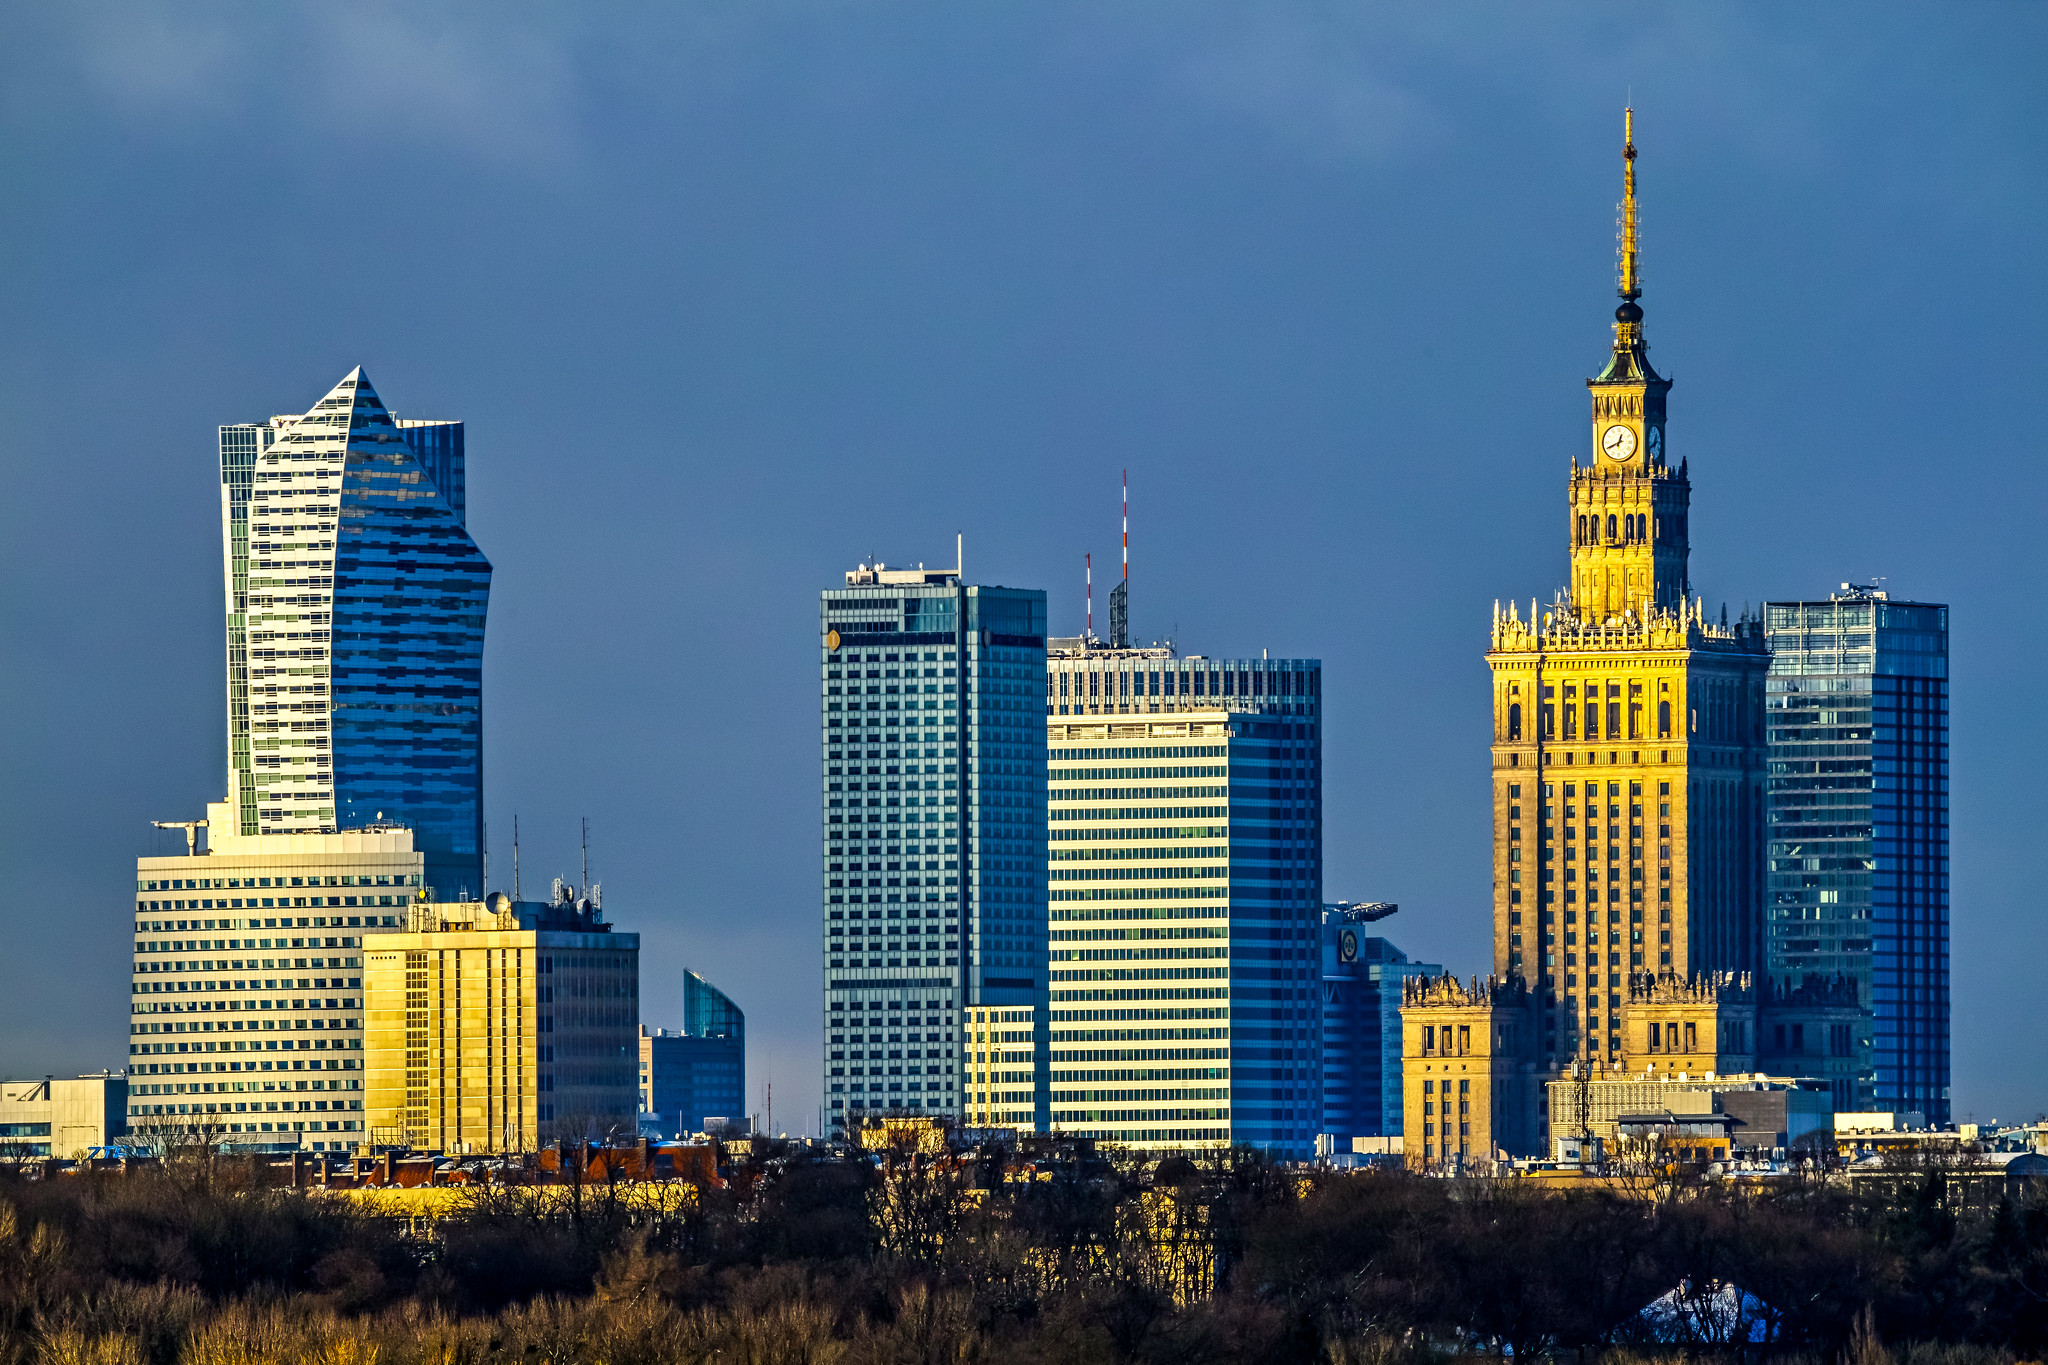
\includegraphics{figure/am1974_flicker.jpg}
\caption{Warsaw skyscrapers by Artur Malinowski Flicker}
\end{figure}

Predicting house prices is a common exercise used in machine-learning
courses. Various datasets for house prices are available at websites
like Kaggle (\url{https://www.kaggle.com}) or UCI Machine Learning
Repository (\url{https://archive.ics.uci.edu}).

In this book, we will work with an interesting variant of this problem.
The \texttt{apartments} dataset is an artificial dataset created to
match key characteristics of real apartments in Warszawa, the capital of
Poland. However, the dataset is created in a way that two very different
models, namely linear regression and random forest, have almost exactly
the same accuracy. The natural question is then: which model should we
choose? We will show that the model-explanation tools provide important
insight into the key model characteristics and are helpful in model
selection.

The dataset is available in the \texttt{DALEX} package \citep{R-DALEX}.
It contains 1000 observations (apartments) and six variables:

\begin{itemize}
\tightlist
\item
  \emph{m2.price}, apatments price per meter-squared (in EUR), a
  numerical variable;
\item
  \emph{construction.year}, the year of construction of the block of
  flats in which the apartment is located, a numerical variable;
\item
  \emph{surface}, apartment's total surface in squared meters, a
  numerical variable;
\item
  \emph{floor}, the floor at which the apartment is located (ground
  floor taken to be the first floor), a numerical integer variable with
  values from 1 to 10;
\item
  \emph{no.rooms}, the total number of rooms, a numerical variable with
  values from 1 to 6;
\item
  \emph{distric}, a factor with 10 levels indicating tha distric of
  Warszawa where the apartment is located.
\end{itemize}

The R code below provides more info about the contents of the dataset,
values of the variables, etc.

\begin{Shaded}
\begin{Highlighting}[]
\KeywordTok{library}\NormalTok{(}\StringTok{"DALEX"}\NormalTok{)}
\KeywordTok{head}\NormalTok{(apartments, }\DecValTok{2}\NormalTok{)}
\end{Highlighting}
\end{Shaded}

\begin{verbatim}
##   m2.price construction.year surface floor no.rooms    district
## 1     5897              1953      25     3        1 Srodmiescie
## 2     1818              1992     143     9        5     Bielany
\end{verbatim}

\begin{Shaded}
\begin{Highlighting}[]
\KeywordTok{str}\NormalTok{(apartments)}
\end{Highlighting}
\end{Shaded}

\begin{verbatim}
## 'data.frame':    1000 obs. of  6 variables:
##  $ m2.price         : num  5897 1818 3643 3517 3013 ...
##  $ construction.year: num  1953 1992 1937 1995 1992 ...
##  $ surface          : num  25 143 56 93 144 61 127 105 145 112 ...
##  $ floor            : int  3 9 1 7 6 6 8 8 6 9 ...
##  $ no.rooms         : num  1 5 2 3 5 2 5 4 6 4 ...
##  $ district         : Factor w/ 10 levels "Bemowo","Bielany",..: 6 2 5 4 3 6 3 7 6 6 ...
\end{verbatim}

\begin{Shaded}
\begin{Highlighting}[]
\KeywordTok{table}\NormalTok{(apartments}\OperatorTok{$}\NormalTok{floor)}
\end{Highlighting}
\end{Shaded}

\begin{verbatim}
## 
##   1   2   3   4   5   6   7   8   9  10 
##  90 116  87  86  95 104 103 103 108 108
\end{verbatim}

\begin{Shaded}
\begin{Highlighting}[]
\KeywordTok{table}\NormalTok{(apartments}\OperatorTok{$}\NormalTok{no.rooms)}
\end{Highlighting}
\end{Shaded}

\begin{verbatim}
## 
##   1   2   3   4   5   6 
##  99 202 231 223 198  47
\end{verbatim}

\begin{Shaded}
\begin{Highlighting}[]
\KeywordTok{levels}\NormalTok{(apartments}\OperatorTok{$}\NormalTok{district)}
\end{Highlighting}
\end{Shaded}

\begin{verbatim}
##  [1] "Bemowo"      "Bielany"     "Mokotow"     "Ochota"      "Praga"      
##  [6] "Srodmiescie" "Ursus"       "Ursynow"     "Wola"        "Zoliborz"
\end{verbatim}

Models considered for this dataset will use \emph{m2.price} as the
(continuous) dependent variable.

Model predictions will be obtained for a set of six apartments included
in data frame \texttt{apartments\_test}, also included in the
\texttt{DALEX} package.

\begin{Shaded}
\begin{Highlighting}[]
\KeywordTok{head}\NormalTok{(apartments_test)}
\end{Highlighting}
\end{Shaded}

\begin{verbatim}
##      m2.price construction.year surface floor no.rooms    district
## 1001     4644              1976     131     3        5 Srodmiescie
## 1002     3082              1978     112     9        4     Mokotow
## 1003     2498              1958     100     7        4     Bielany
## 1004     2735              1951     112     3        5        Wola
## 1005     2781              1978     102     4        4      Bemowo
## 1006     2936              2001     116     7        4      Bemowo
\end{verbatim}

\hypertarget{exploration-apartments}{%
\subsubsection{Data exploration}\label{exploration-apartments}}

Note that \texttt{apartments} is an artificial dataset created to
illustrate and explain differences between random forest and linear
regression. Hence, the structure of the data, the form and strength of
association between variables, plausibility of distributional
assumptions, etc., is better than in a real-life dataset. In fact, all
these characteristics of the data are known. Nevertheless, we conduct
some data exploration to illustrate the important aspects of the data.

The variable of interest is \emph{m2.price}, the price per
meter-squared. The histogram presented in Figure
\ref{fig:appartmentsExplorationMi2} indicates that the distribution of
the variable is slightly skewed to the right.
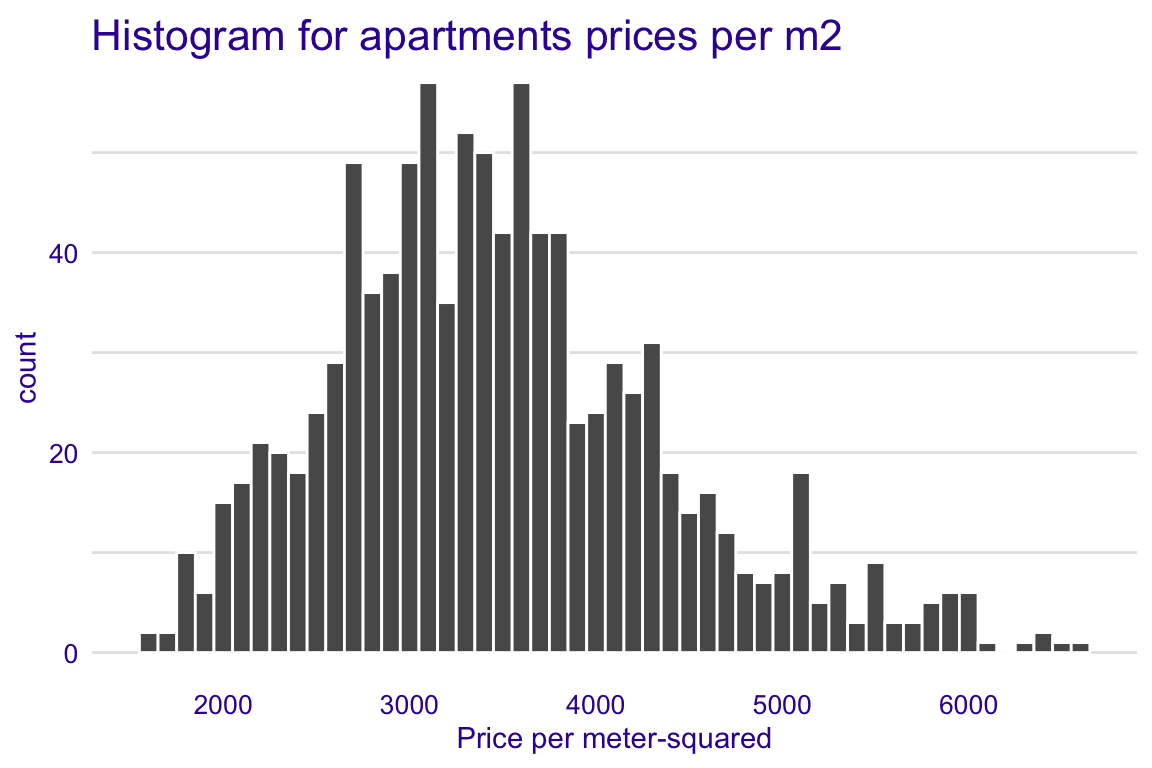
\includegraphics{PM_VEE_files/figure-latex/appartmentsExplorationMi2-1.pdf}

Figure \ref{fig:appartmentsMi2Construction} suggests (possibly) a
nonlinear relation between \emph{construction.year} and \emph{m2.price}.

\begin{figure}
\centering
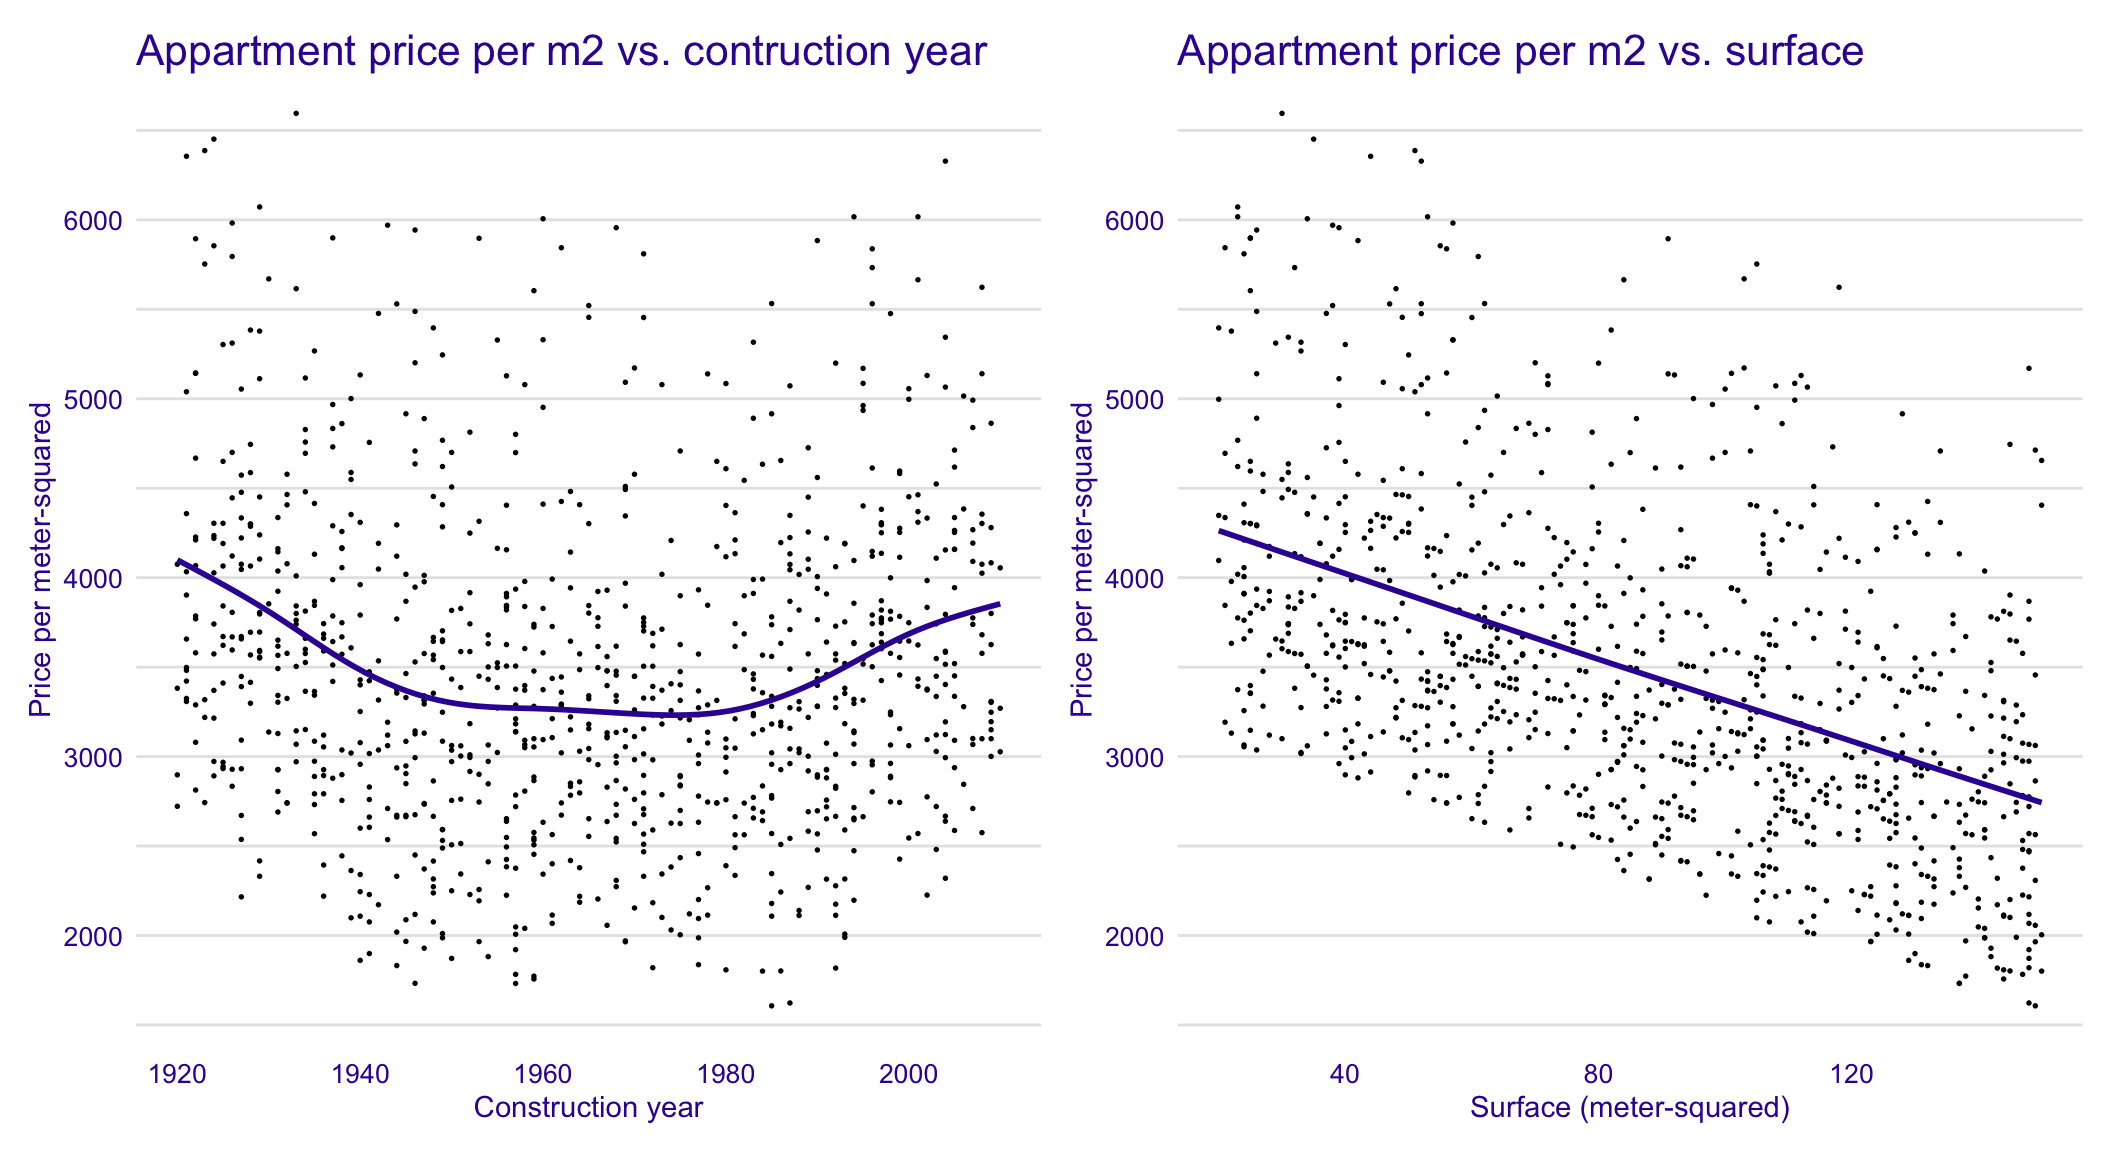
\includegraphics{PM_VEE_files/figure-latex/appartmentsMi2Construction-1.pdf}
\caption{\label{fig:appartmentsMi2Construction}(fig:appartmentsMi2Construction)
Price per meter-squared vs.~construction year}
\end{figure}

Figure \ref{fig:appartmentsMi2Surface} indicates a linear relation
between \emph{surface} and \emph{m2.price}.

\begin{figure}
\centering
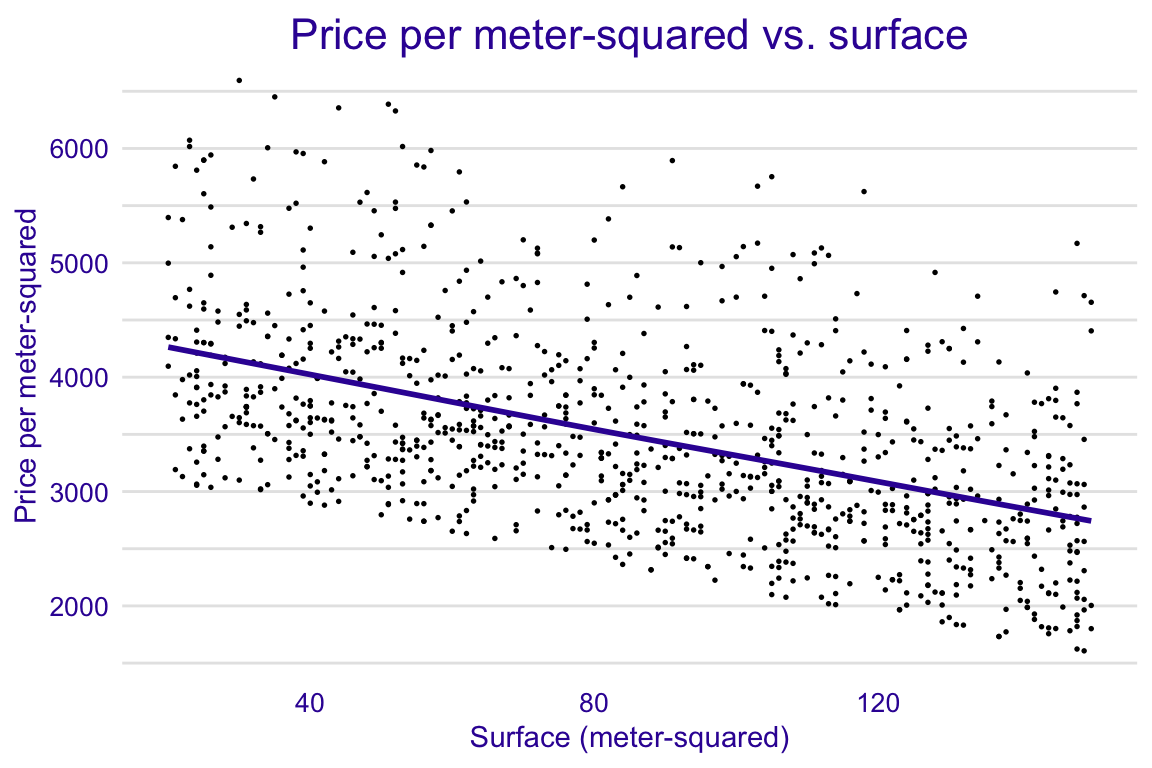
\includegraphics{PM_VEE_files/figure-latex/appartmentsMi2Surface-1.pdf}
\caption{\label{fig:appartmentsMi2Surface}(fig:appartmentsMi2Surface) Price
per meter-squared vs.~surface}
\end{figure}

Relation between \emph{floor} and \emph{m2.price} is also close to
linear, as seen in Figure \ref{fig:appartmentsMi2Floor}.

\begin{figure}
\centering
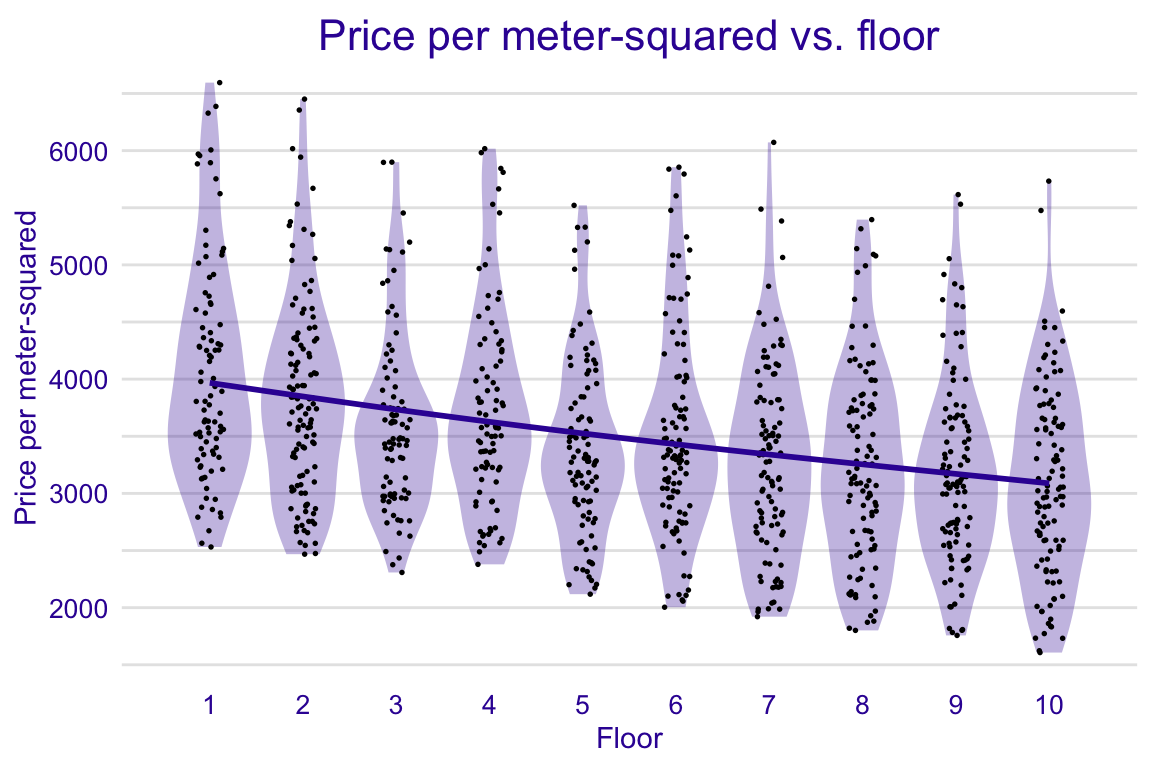
\includegraphics{PM_VEE_files/figure-latex/appartmentsMi2Floor-1.pdf}
\caption{\label{fig:appartmentsMi2Floor}(fig:appartmentsMi2Floor) Price per
meter-squared vs.~floor}
\end{figure}

There is a close to linear relation between \emph{no.rooms} and
\emph{m2.price}, as suggested by Figure \ref{fig:appartmentsMi2Norooms}.
It is worth noting that, quite naturally, surface and number of rooms
are correlated (see Figure \ref{fig:appartmentsSurfaceNorooms}).

\begin{figure}
\centering
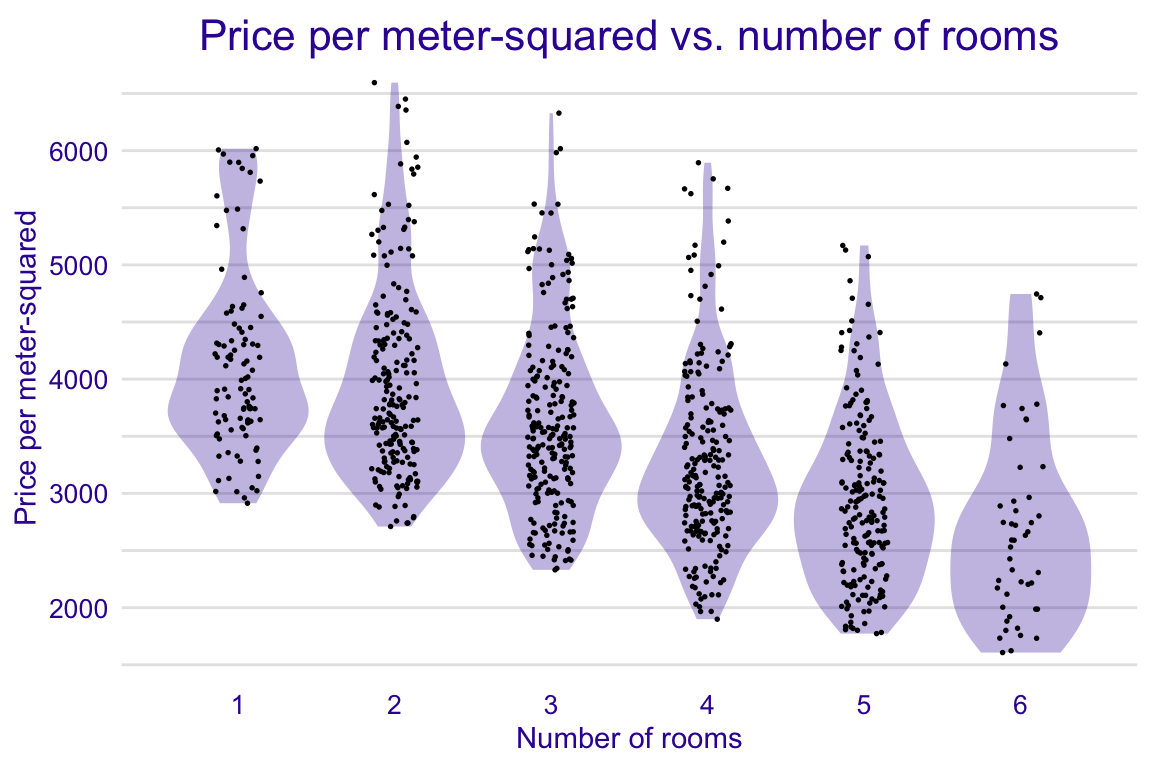
\includegraphics{PM_VEE_files/figure-latex/appartmentsMi2Norooms-1.pdf}
\caption{\label{fig:appartmentsMi2Norooms}(fig:appartmentsMi2Norooms) Price
per meter-squared vs.~number of rooms}
\end{figure}

\begin{figure}
\centering
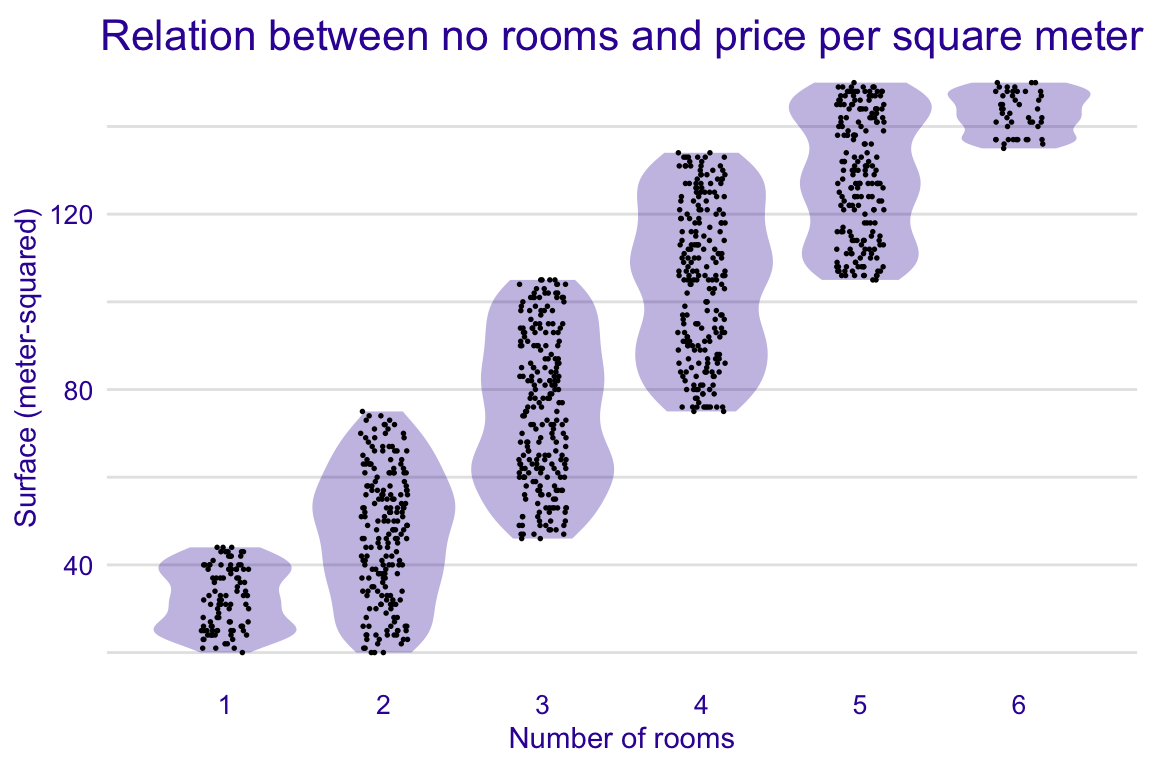
\includegraphics{PM_VEE_files/figure-latex/appartmentsSurfaceNorooms-1.pdf}
\caption{\label{fig:appartmentsSurfaceNorooms}(fig:appartmentsSurfaceNorooms)
Surface vs.~number of rooms}
\end{figure}

Prices depend on district. Violin plots in Figure
\ref{fig:appartmentsMi2District} indicate that the highest prices per
meter-squared are observed in Srodmiescie (Downtown).

\begin{figure}
\centering
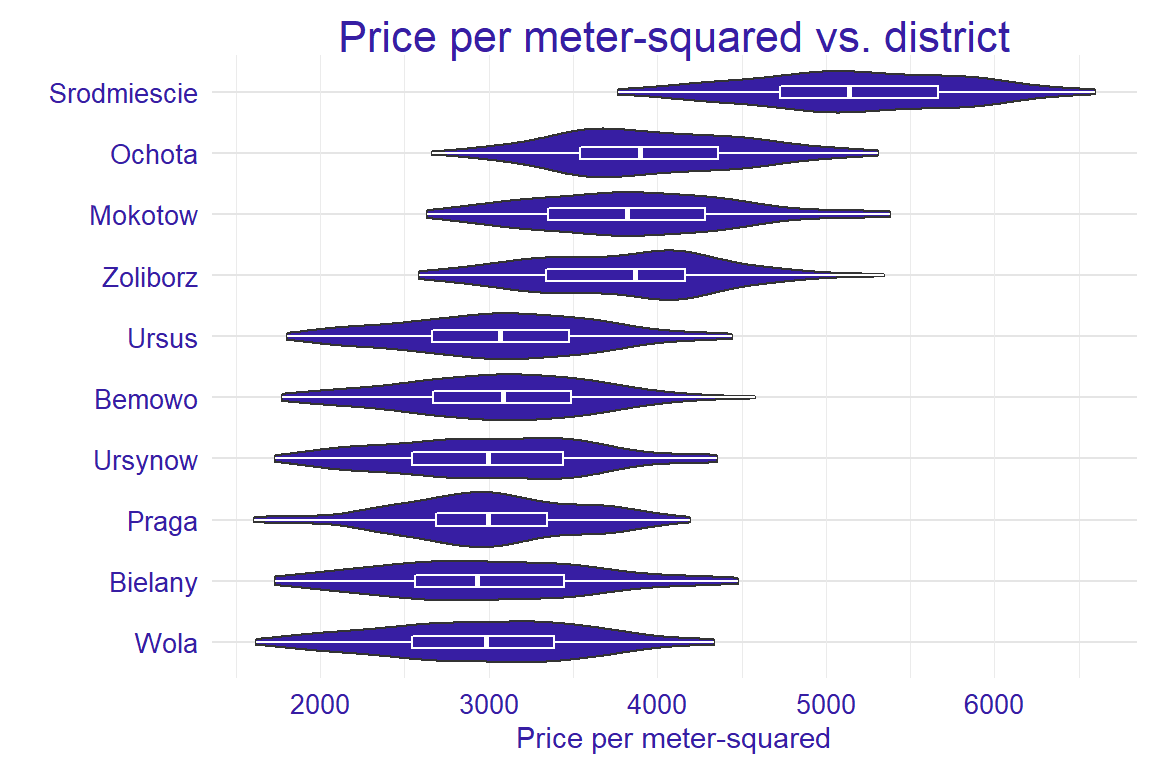
\includegraphics{PM_VEE_files/figure-latex/appartmentsMi2District-1.pdf}
\caption{\label{fig:appartmentsMi2District}(fig:appartmentsMi2District)
Price per meter-squared for different districts}
\end{figure}

\hypertarget{model-Apartments-lr}{%
\subsubsection{Linear regression}\label{model-Apartments-lr}}

The dependent variable of interest, \emph{m2.price}, is continuous.
Thus, a natural choice to build a predictive model is linear regression.
We treat all the other variables in the \texttt{apartments} data frame
as explanatory and include them in the model. The results of the model
are stored in model-object \texttt{apartments\_lm\_v5}.

\begin{Shaded}
\begin{Highlighting}[]
\NormalTok{apartments_lm_v5 <-}\StringTok{ }\KeywordTok{lm}\NormalTok{(m2.price }\OperatorTok{~}\StringTok{ }\NormalTok{., }\DataTypeTok{data =}\NormalTok{ apartments)}
\NormalTok{apartments_lm_v5}
\end{Highlighting}
\end{Shaded}

\begin{verbatim}
## 
## Call:
## lm(formula = m2.price ~ ., data = apartments)
## 
## Coefficients:
##         (Intercept)    construction.year              surface  
##            5003.248               -0.229              -10.238  
##               floor             no.rooms      districtBielany  
##             -99.482              -37.730               34.106  
##       districtPraga      districtUrsynow       districtBemowo  
##             -20.214               -1.974               16.891  
##       districtUrsus     districtZoliborz      districtMokotow  
##              46.833              906.865              935.271  
##      districtOchota  districtSrodmiescie  
##             943.145             2097.502
\end{verbatim}

\hypertarget{model-Apartments-rf}{%
\subsubsection{Random forest}\label{model-Apartments-rf}}

As an alternative to linear regression, we consider a random forest
model. To fit the model, we apply the \texttt{randomForest()} function,
with default settings, from the package with the same name
\citep{randomForestRNews}.\\
The results of the model are stored in model-object
\texttt{apartments\_rf\_v5}.

\begin{Shaded}
\begin{Highlighting}[]
\KeywordTok{library}\NormalTok{(}\StringTok{"randomForest"}\NormalTok{)}
\KeywordTok{set.seed}\NormalTok{(}\DecValTok{72}\NormalTok{)}
\NormalTok{apartments_rf_v5 <-}\StringTok{ }\KeywordTok{randomForest}\NormalTok{(m2.price }\OperatorTok{~}\StringTok{ }\NormalTok{., }\DataTypeTok{data =}\NormalTok{ apartments)}
\NormalTok{apartments_rf_v5}
\end{Highlighting}
\end{Shaded}

\begin{verbatim}
## 
## Call:
##  randomForest(formula = m2.price ~ ., data = apartments) 
##                Type of random forest: regression
##                      Number of trees: 500
## No. of variables tried at each split: 1
## 
##           Mean of squared residuals: 79789.39
##                     % Var explained: 90.28
\end{verbatim}

\hypertarget{predictionsApartments}{%
\subsubsection{Model predictions}\label{predictionsApartments}}

By aplying the \texttt{predict()} function to model-object
\texttt{apartments\_lm\_v5} with \texttt{apartments\_test} as the data
frame for which predictions are to be computed, we obtain the predicted
prices for the testing set of six apartments for the linear regression
model. Subsequently, we compute the mean squared difference between the
predicted and actual prices for the test apartments. We repeat the same
steps for the random forest model.

\begin{Shaded}
\begin{Highlighting}[]
\NormalTok{predicted_apartments_lm <-}\StringTok{ }\KeywordTok{predict}\NormalTok{(apartments_lm_v5, apartments_test)}
\NormalTok{rmsd_lm <-}\StringTok{ }\KeywordTok{sqrt}\NormalTok{(}\KeywordTok{mean}\NormalTok{((predicted_apartments_lm }\OperatorTok{-}\StringTok{ }\NormalTok{apartments_test}\OperatorTok{$}\NormalTok{m2.price)}\OperatorTok{^}\DecValTok{2}\NormalTok{))}
\NormalTok{rmsd_lm}
\end{Highlighting}
\end{Shaded}

\begin{verbatim}
## [1] 283.0865
\end{verbatim}

\begin{Shaded}
\begin{Highlighting}[]
\NormalTok{predicted_apartments_rf <-}\StringTok{ }\KeywordTok{predict}\NormalTok{(apartments_rf_v5, apartments_test)}
\NormalTok{rmsd_rf <-}\StringTok{ }\KeywordTok{sqrt}\NormalTok{(}\KeywordTok{mean}\NormalTok{((predicted_apartments_rf }\OperatorTok{-}\StringTok{ }\NormalTok{apartments_test}\OperatorTok{$}\NormalTok{m2.price)}\OperatorTok{^}\DecValTok{2}\NormalTok{))}
\NormalTok{rmsd_rf}
\end{Highlighting}
\end{Shaded}

\begin{verbatim}
## [1] 282.9519
\end{verbatim}

For the random forest model, the square-root of the mean squared
difference is equal to 283. It is only minimally smaller than the value
of 283.1, obtained for the linear regression model. Thus, the question
we may face is: should we choose the more complex, but flexible
random-forest model, or the simpler and easier to interpret linear
model? In the subsequent chapters we will try to provide an answer to
this question.

\hypertarget{ListOfModelsApartments}{%
\subsubsection{\texorpdfstring{List of objects for the
\texttt{apartments}
example}{List of objects for the apartments example}}\label{ListOfModelsApartments}}

In Sections \ref{model-Apartments-lr} and \ref{model-Apartments-rf} we
have built two predictive models for the \texttt{apartments} data set.
The models will be used in the rest of the book to illustrate the model
explanation methods and tools.

For the ease of reference, we summarize the models in Table
\ref{tab:archivistHooksOfModelsApartments}. The binary model-objects can
be downloaded by using the indicated \texttt{archivist} hooks
\citep{archivist}. By calling a function specified in the last column of
the table, one can recreate a selected model in a local R environment.

\begin{longtable}[]{@{}llll@{}}
\caption{\label{tab:archivistHooksOfModelsApartments} Predictive models
created for the \texttt{apartments} dataset.}\tabularnewline
\toprule
\begin{minipage}[b]{0.21\columnwidth}\raggedright
Model name\strut
\end{minipage} & \begin{minipage}[b]{0.25\columnwidth}\raggedright
Model generator\strut
\end{minipage} & \begin{minipage}[b]{0.18\columnwidth}\raggedright
Variables\strut
\end{minipage} & \begin{minipage}[b]{0.25\columnwidth}\raggedright
Archivist hooks\strut
\end{minipage}\tabularnewline
\midrule
\endfirsthead
\toprule
\begin{minipage}[b]{0.21\columnwidth}\raggedright
Model name\strut
\end{minipage} & \begin{minipage}[b]{0.25\columnwidth}\raggedright
Model generator\strut
\end{minipage} & \begin{minipage}[b]{0.18\columnwidth}\raggedright
Variables\strut
\end{minipage} & \begin{minipage}[b]{0.25\columnwidth}\raggedright
Archivist hooks\strut
\end{minipage}\tabularnewline
\midrule
\endhead
\begin{minipage}[t]{0.21\columnwidth}\raggedright
\texttt{apartments\_lm\_v5}\strut
\end{minipage} & \begin{minipage}[t]{0.25\columnwidth}\raggedright
\texttt{stats::\ lm} v.3.5.3\strut
\end{minipage} & \begin{minipage}[t]{0.18\columnwidth}\raggedright
construction .year, surface, floor, no.rooms, district\strut
\end{minipage} & \begin{minipage}[t]{0.25\columnwidth}\raggedright
Get the model: \texttt{archivist::\ aread("pbiecek/models/55f19")}. Get
the explainer: TODO: add if needed\strut
\end{minipage}\tabularnewline
\begin{minipage}[t]{0.21\columnwidth}\raggedright
\texttt{apartments\_rf\_v5}\strut
\end{minipage} & \begin{minipage}[t]{0.25\columnwidth}\raggedright
\texttt{randomForest::\ randomForest} v.4.6.14\strut
\end{minipage} & \begin{minipage}[t]{0.18\columnwidth}\raggedright
construction .year, surface, floor, no.rooms, district\strut
\end{minipage} & \begin{minipage}[t]{0.25\columnwidth}\raggedright
Get the model: \texttt{archivist::\ aread("pbiecek/models/fe7a5")}. Get
the explainer: TODO: add if needed\strut
\end{minipage}\tabularnewline
\bottomrule
\end{longtable}

\hypertarget{HFDataset}{%
\subsection{Hire or fire}\label{HFDataset}}

Predictive models can be used to support decisions. For instance, they
can be used in a human-resources department to decide whether, for
instance, to promote an employee. An advantage of using a model for this
purpose would be the objectivity of the decision, which would not be
subject to personal preferences of a manager. However, in such a
situation, one would most likely want to understand what influences the
model's prediction.

To illustrate such a situation, we will use the \texttt{HR} dataset that
is available in the \texttt{DALEX} package \citep{R-DALEX}. It is an
artificial set of data from a human-resources department of a call
center. It contains 7847 observations (employees of the call center) and
six variables:

\begin{itemize}
\tightlist
\item
  \emph{gender}, person's gender, a factor with two levels;
\item
  \emph{age}, person's age in years, a numerical variable;
\item
  \emph{hours}, average number of working hours per week, a numerical
  variable;
\item
  \emph{evaluation}, the last evaluation score, a numerical variable
  with values 2 (fail), 3 (satisfactory), 4 (good), and 5 (very good);
\item
  \emph{salary}, the salary level, a numerical variable with values from
  0 (lowest) to 5 (highest);
\item
  \emph{status}, a factor with three indicating whether the employee was
  fired, retained, or promoted.
\end{itemize}

The R code below provides more info about the contents of the dataset,
values of the variables, etc.

\begin{Shaded}
\begin{Highlighting}[]
\KeywordTok{library}\NormalTok{(}\StringTok{"DALEX"}\NormalTok{)}
\KeywordTok{head}\NormalTok{(HR, }\DecValTok{4}\NormalTok{)}
\end{Highlighting}
\end{Shaded}

\begin{verbatim}
##   gender      age    hours evaluation salary status
## 1   male 32.58267 41.88626          3      1  fired
## 2 female 41.21104 36.34339          2      5  fired
## 3   male 37.70516 36.81718          3      0  fired
## 4 female 30.06051 38.96032          3      2  fired
\end{verbatim}

\begin{Shaded}
\begin{Highlighting}[]
\KeywordTok{str}\NormalTok{(HR)}
\end{Highlighting}
\end{Shaded}

\begin{verbatim}
## 'data.frame':    7847 obs. of  6 variables:
##  $ gender    : Factor w/ 2 levels "female","male": 2 1 2 1 2 2 1 2 1 1 ...
##  $ age       : num  32.6 41.2 37.7 30.1 21.1 ...
##  $ hours     : num  41.9 36.3 36.8 39 62.2 ...
##  $ evaluation: num  3 2 3 3 5 2 4 2 2 4 ...
##  $ salary    : num  1 5 0 2 3 0 0 4 4 4 ...
##  $ status    : Factor w/ 3 levels "fired","ok","promoted": 1 1 1 1 3 1 3 2 1 3 ...
\end{verbatim}

\begin{Shaded}
\begin{Highlighting}[]
\KeywordTok{table}\NormalTok{(HR}\OperatorTok{$}\NormalTok{evaluation)}
\end{Highlighting}
\end{Shaded}

\begin{verbatim}
## 
##    2    3    4    5 
## 2371 2272 1661 1543
\end{verbatim}

\begin{Shaded}
\begin{Highlighting}[]
\KeywordTok{table}\NormalTok{(HR}\OperatorTok{$}\NormalTok{salary)}
\end{Highlighting}
\end{Shaded}

\begin{verbatim}
## 
##    0    1    2    3    4    5 
## 1105 1417 1461 1508 1316 1040
\end{verbatim}

Models considered for this dataset will use \emph{status} as the
(categorical) dependent variable.

\hypertarget{exploration-HR}{%
\subsubsection{Data exploration}\label{exploration-HR}}

As it was the case for the \texttt{apartments} dataset (see Section
\ref{ApartmentDataset}), the \texttt{HR} data were simulated. Despite
the fact that characteristics of the data are known, we conduct some
data exploration to illustrate the important aspects of the data.

Figure \ref{fig:HRExplorationAge} indicates that young females and older
males were fired more frequently than older females and younger males.

\begin{figure}

{\centering 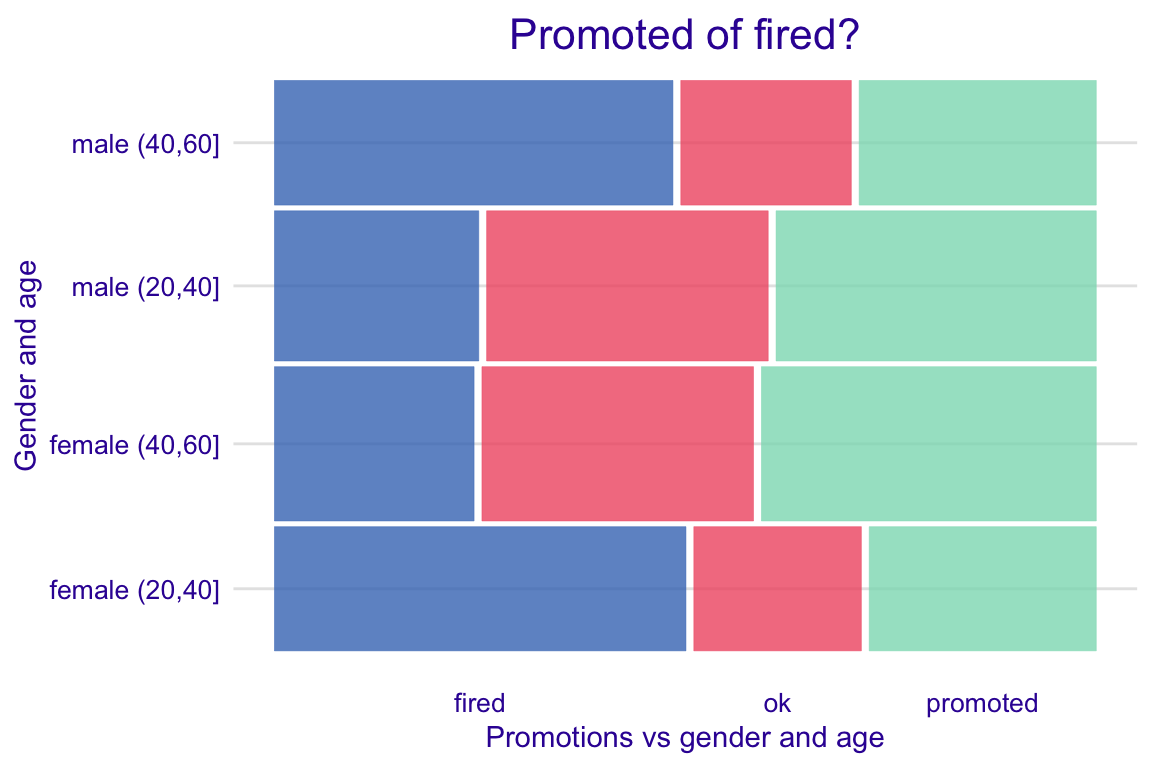
\includegraphics[width=0.7\linewidth]{PM_VEE_files/figure-latex/HRExplorationAge-1} 

}

\caption{Employment status for age-groups and gender.}\label{fig:HRExplorationAge}
\end{figure}

Figure \ref{fig:HRExplorationSalary} indicates that the proportion of
promoted employees was the lowest for the lowest and highest salary
level. At the same time, the proportion of fired employees was the
highest for the two salary levels.

\begin{figure}

{\centering 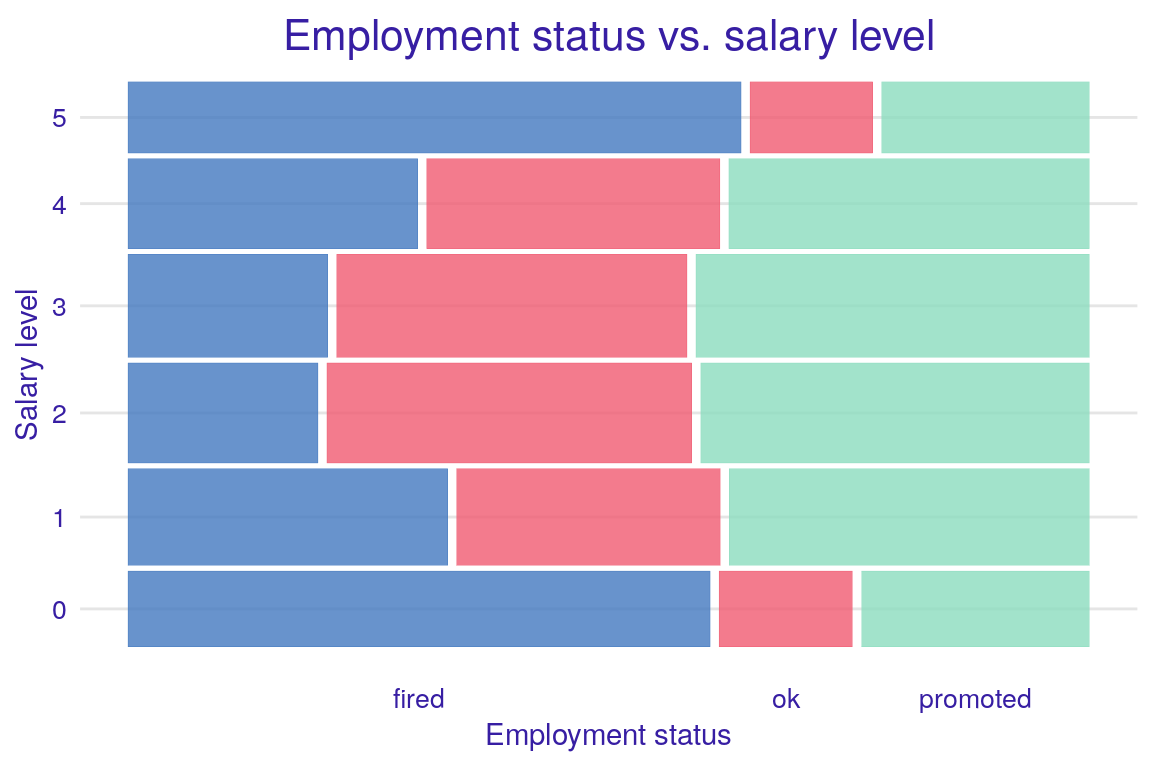
\includegraphics[width=0.7\linewidth]{PM_VEE_files/figure-latex/HRExplorationSalary-1} 

}

\caption{Employment status for different salary levels.}\label{fig:HRExplorationSalary}
\end{figure}

Figure \ref{fig:HRExplorationEvaluation} indicates that the chance of
being fired was larger for evaluation scores equal to 2 or 3. On the
other hand, the chance of being promoted substantially increased for
scores equal to 4 or 5.\\

\begin{figure}

{\centering 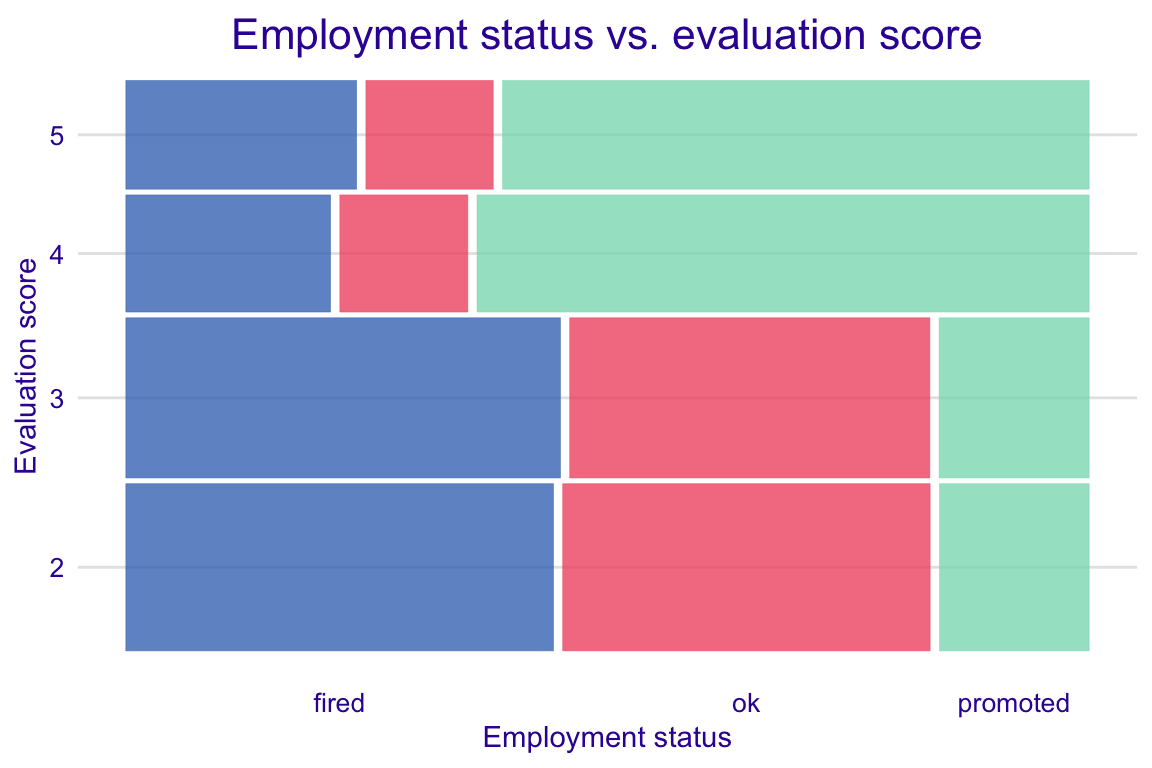
\includegraphics[width=0.7\linewidth]{PM_VEE_files/figure-latex/HRExplorationEvaluation-1} 

}

\caption{Employment status for different evaluation scores.}\label{fig:HRExplorationEvaluation}
\end{figure}

\hypertarget{model-HR-mr}{%
\subsubsection{Multinomial logistic regression}\label{model-HR-mr}}

The dependent variable of interest, \emph{status}, is categorical with
three categories. Thus, a simple choice is to consider a multinomial
logistic regression model \citep{Venables2010}. We fit the model with
the help of function \texttt{multinom} from package \texttt{nnet}. The
function fits multinomial log-linear models by using the neural-networks
approach. As a result, we obtain a complex model that is smoother as
compared to a random forest model that relies on binary splits for
continuous variables. We treat all variables other than \texttt{status}
in the \texttt{HR} data frame as explanatory and include them in the
model. The results of the model are stored in model-object
\texttt{HR\_glm\_v5}.

\begin{Shaded}
\begin{Highlighting}[]
\KeywordTok{library}\NormalTok{(}\StringTok{"nnet"}\NormalTok{)}
\KeywordTok{set.seed}\NormalTok{(}\DecValTok{1313}\NormalTok{)}
\NormalTok{HR_glm_v5 <-}\StringTok{ }\KeywordTok{multinom}\NormalTok{(status }\OperatorTok{~}\StringTok{ }\NormalTok{gender }\OperatorTok{+}\StringTok{ }\NormalTok{age }\OperatorTok{+}\StringTok{ }\NormalTok{hours }\OperatorTok{+}\StringTok{ }\NormalTok{evaluation }\OperatorTok{+}\StringTok{ }\NormalTok{salary, }\DataTypeTok{data =}\NormalTok{ HR)}
\end{Highlighting}
\end{Shaded}

\begin{verbatim}
## # weights:  21 (12 variable)
## initial  value 8620.810629 
## iter  10 value 7002.127738
## iter  20 value 6239.478146
## iter  20 value 6239.478126
## iter  20 value 6239.478124
## final  value 6239.478124 
## converged
\end{verbatim}

\begin{Shaded}
\begin{Highlighting}[]
\NormalTok{HR_glm_v5}
\end{Highlighting}
\end{Shaded}

\begin{verbatim}
## Call:
## multinom(formula = status ~ gender + age + hours + evaluation + 
##     salary, data = HR)
## 
## Coefficients:
##          (Intercept) gendermale         age      hours  evaluation
## ok         -3.199741 0.05185293 0.001003521 0.06628055 -0.03734345
## promoted  -12.677639 0.11838037 0.003436872 0.16253343  1.26109093
##              salary
## ok       0.01680039
## promoted 0.01507927
## 
## Residual Deviance: 12478.96 
## AIC: 12502.96
\end{verbatim}

\hypertarget{model-HR-rf}{%
\subsubsection{Random forest}\label{model-HR-rf}}

As an alternative to multinomial logistic regression, we consider a
random forest model. To fit the model, we apply the
\texttt{randomForest()} function, with default settings, from the
package with the same name \citep{randomForestRNews}. The results of the
model are stored in model-object \texttt{HR\_rf\_v5}.

\begin{Shaded}
\begin{Highlighting}[]
\KeywordTok{library}\NormalTok{(}\StringTok{"randomForest"}\NormalTok{)}
\KeywordTok{set.seed}\NormalTok{(}\DecValTok{1313}\NormalTok{)}
\NormalTok{HR_rf_v5 <-}\StringTok{ }\KeywordTok{randomForest}\NormalTok{(status }\OperatorTok{~}\StringTok{ }\NormalTok{gender }\OperatorTok{+}\StringTok{ }\NormalTok{age }\OperatorTok{+}\StringTok{ }\NormalTok{hours }\OperatorTok{+}\StringTok{ }\NormalTok{evaluation }\OperatorTok{+}\StringTok{ }\NormalTok{salary, }\DataTypeTok{data =}\NormalTok{ HR)}
\NormalTok{HR_rf_v5}
\end{Highlighting}
\end{Shaded}

\begin{verbatim}
## 
## Call:
##  randomForest(formula = status ~ gender + age + hours + evaluation +      salary, data = HR) 
##                Type of random forest: classification
##                      Number of trees: 500
## No. of variables tried at each split: 2
## 
##         OOB estimate of  error rate: 27.46%
## Confusion matrix:
##          fired   ok promoted class.error
## fired     2270  388      197   0.2049037
## ok         530 1243      448   0.4403422
## promoted   202  390     2179   0.2136413
\end{verbatim}

\hypertarget{predictionsHR}{%
\subsubsection{Model predictions}\label{predictionsHR}}

Let us now compare predictions that are obtained from the multinomial
regression and random forest models. In particular, we compute the
predicted probabilities of being fired, retained in service, or promoted
for Dilbert, a 58-year old male working around 42 hours per week for a
salary at level 2, who got evaluation score equal to 2. Data frame
\texttt{dilbert} contains the data describing the employee.

\begin{Shaded}
\begin{Highlighting}[]
\NormalTok{dilbert <-}\StringTok{ }\KeywordTok{data.frame}\NormalTok{(}\DataTypeTok{gender =} \KeywordTok{factor}\NormalTok{(}\StringTok{"male"}\NormalTok{, }\DataTypeTok{levels =} \KeywordTok{c}\NormalTok{(}\StringTok{"male"}\NormalTok{, }\StringTok{"female"}\NormalTok{)),}
                \DataTypeTok{age =} \FloatTok{57.7}\NormalTok{,}
                \DataTypeTok{hours =} \FloatTok{42.3}\NormalTok{,}
                \DataTypeTok{evaluation =} \DecValTok{2}\NormalTok{,}
                \DataTypeTok{salary =} \DecValTok{2}\NormalTok{)}
\end{Highlighting}
\end{Shaded}

By aplying the \texttt{predict()} function to model-objects
\texttt{HR\_rf\_v5} and \texttt{HR\_glm\_v5}, with \texttt{dilbert} as
the data frame for which predictions are to be computed, and argument
\texttt{type="prob"}, we obtain the predicted probabilities of being
fired, retained in service, or promoted for Dilbert.

\begin{Shaded}
\begin{Highlighting}[]
\NormalTok{pred_HR_rf <-}\StringTok{ }\KeywordTok{predict}\NormalTok{(HR_rf_v5, dilbert, }\DataTypeTok{type =} \StringTok{"prob"}\NormalTok{)}
\NormalTok{pred_HR_rf}
\end{Highlighting}
\end{Shaded}

\begin{verbatim}
##   fired    ok promoted
## 1 0.778 0.218    0.004
## attr(,"class")
## [1] "matrix" "votes"
\end{verbatim}

\begin{Shaded}
\begin{Highlighting}[]
\NormalTok{pred_HR_glm <-}\StringTok{ }\KeywordTok{predict}\NormalTok{(HR_glm_v5, dilbert, }\DataTypeTok{type =} \StringTok{"prob"}\NormalTok{)}
\NormalTok{pred_HR_glm}
\end{Highlighting}
\end{Shaded}

\begin{verbatim}
##      fired         ok   promoted 
## 0.56369601 0.40630786 0.02999612
\end{verbatim}

For both models, the predicted probability of promotion is low; it is
more likely that Dilbert will be fired. It is of interest to understand
why such prediction is made? Moreover, random forest yields a higher
probability of firing (0.78) than the multinomial regression model
(0.56). We may want to learn where does this difference come from? We
will try to answer these questions in subsequent chapters.

\hypertarget{ListOfModelsHR}{%
\subsubsection{\texorpdfstring{List of objects for the \texttt{HR}
example}{List of objects for the HR example}}\label{ListOfModelsHR}}

In Sections \ref{model-HR-mr} and \ref{model-HR-rf} we have built two
predictive models for the \texttt{HR} data set. The models will be used
in the remainder of the book to illustrate model-explanation methods and
tools.

For the ease of reference, we summarize the models in Table
\ref{tab:archivistHooksOfModelsHR}. The binary model-objects can be
downloaded by using the indicated \texttt{archivist} hooks
\citep{archivist}. By calling a function specified in the last column of
the table, one can recreate a selected model in a local R environment.

\begin{longtable}[]{@{}llll@{}}
\caption{\label{tab:archivistHooksOfModelsHR} Predictive models created for
the \texttt{HR} dataset.}\tabularnewline
\toprule
\begin{minipage}[b]{0.21\columnwidth}\raggedright
Model name\strut
\end{minipage} & \begin{minipage}[b]{0.25\columnwidth}\raggedright
Model generator\strut
\end{minipage} & \begin{minipage}[b]{0.18\columnwidth}\raggedright
Variables\strut
\end{minipage} & \begin{minipage}[b]{0.25\columnwidth}\raggedright
Archivist hooks\strut
\end{minipage}\tabularnewline
\midrule
\endfirsthead
\toprule
\begin{minipage}[b]{0.21\columnwidth}\raggedright
Model name\strut
\end{minipage} & \begin{minipage}[b]{0.25\columnwidth}\raggedright
Model generator\strut
\end{minipage} & \begin{minipage}[b]{0.18\columnwidth}\raggedright
Variables\strut
\end{minipage} & \begin{minipage}[b]{0.25\columnwidth}\raggedright
Archivist hooks\strut
\end{minipage}\tabularnewline
\midrule
\endhead
\begin{minipage}[t]{0.21\columnwidth}\raggedright
\texttt{HR\_rf\_v5}\strut
\end{minipage} & \begin{minipage}[t]{0.25\columnwidth}\raggedright
\texttt{randomForest::\ randomForest} v.4.6.14\strut
\end{minipage} & \begin{minipage}[t]{0.18\columnwidth}\raggedright
gender, age, hours, evaluation, salary\strut
\end{minipage} & \begin{minipage}[t]{0.25\columnwidth}\raggedright
Get the model: \texttt{archivist::\ aread("pbiecek/models/1ecfd")}. Get
the explainer: TODO: add if needed\strut
\end{minipage}\tabularnewline
\begin{minipage}[t]{0.21\columnwidth}\raggedright
\texttt{HR\_glm\_v5}\strut
\end{minipage} & \begin{minipage}[t]{0.25\columnwidth}\raggedright
\texttt{stats::\ glm} v.3.5.3\strut
\end{minipage} & \begin{minipage}[t]{0.18\columnwidth}\raggedright
gender, age, hours, evaluation, salary\strut
\end{minipage} & \begin{minipage}[t]{0.25\columnwidth}\raggedright
Get the model: \texttt{archivist::\ aread("pbiecek/models/f0244")}. Get
the explainer: TODO: add if needed\strut
\end{minipage}\tabularnewline
\bottomrule
\end{longtable}

\hypertarget{InstanceLevelExploration}{%
\section{Instance-level exploration}\label{InstanceLevelExploration}}

\begin{figure}

{\centering 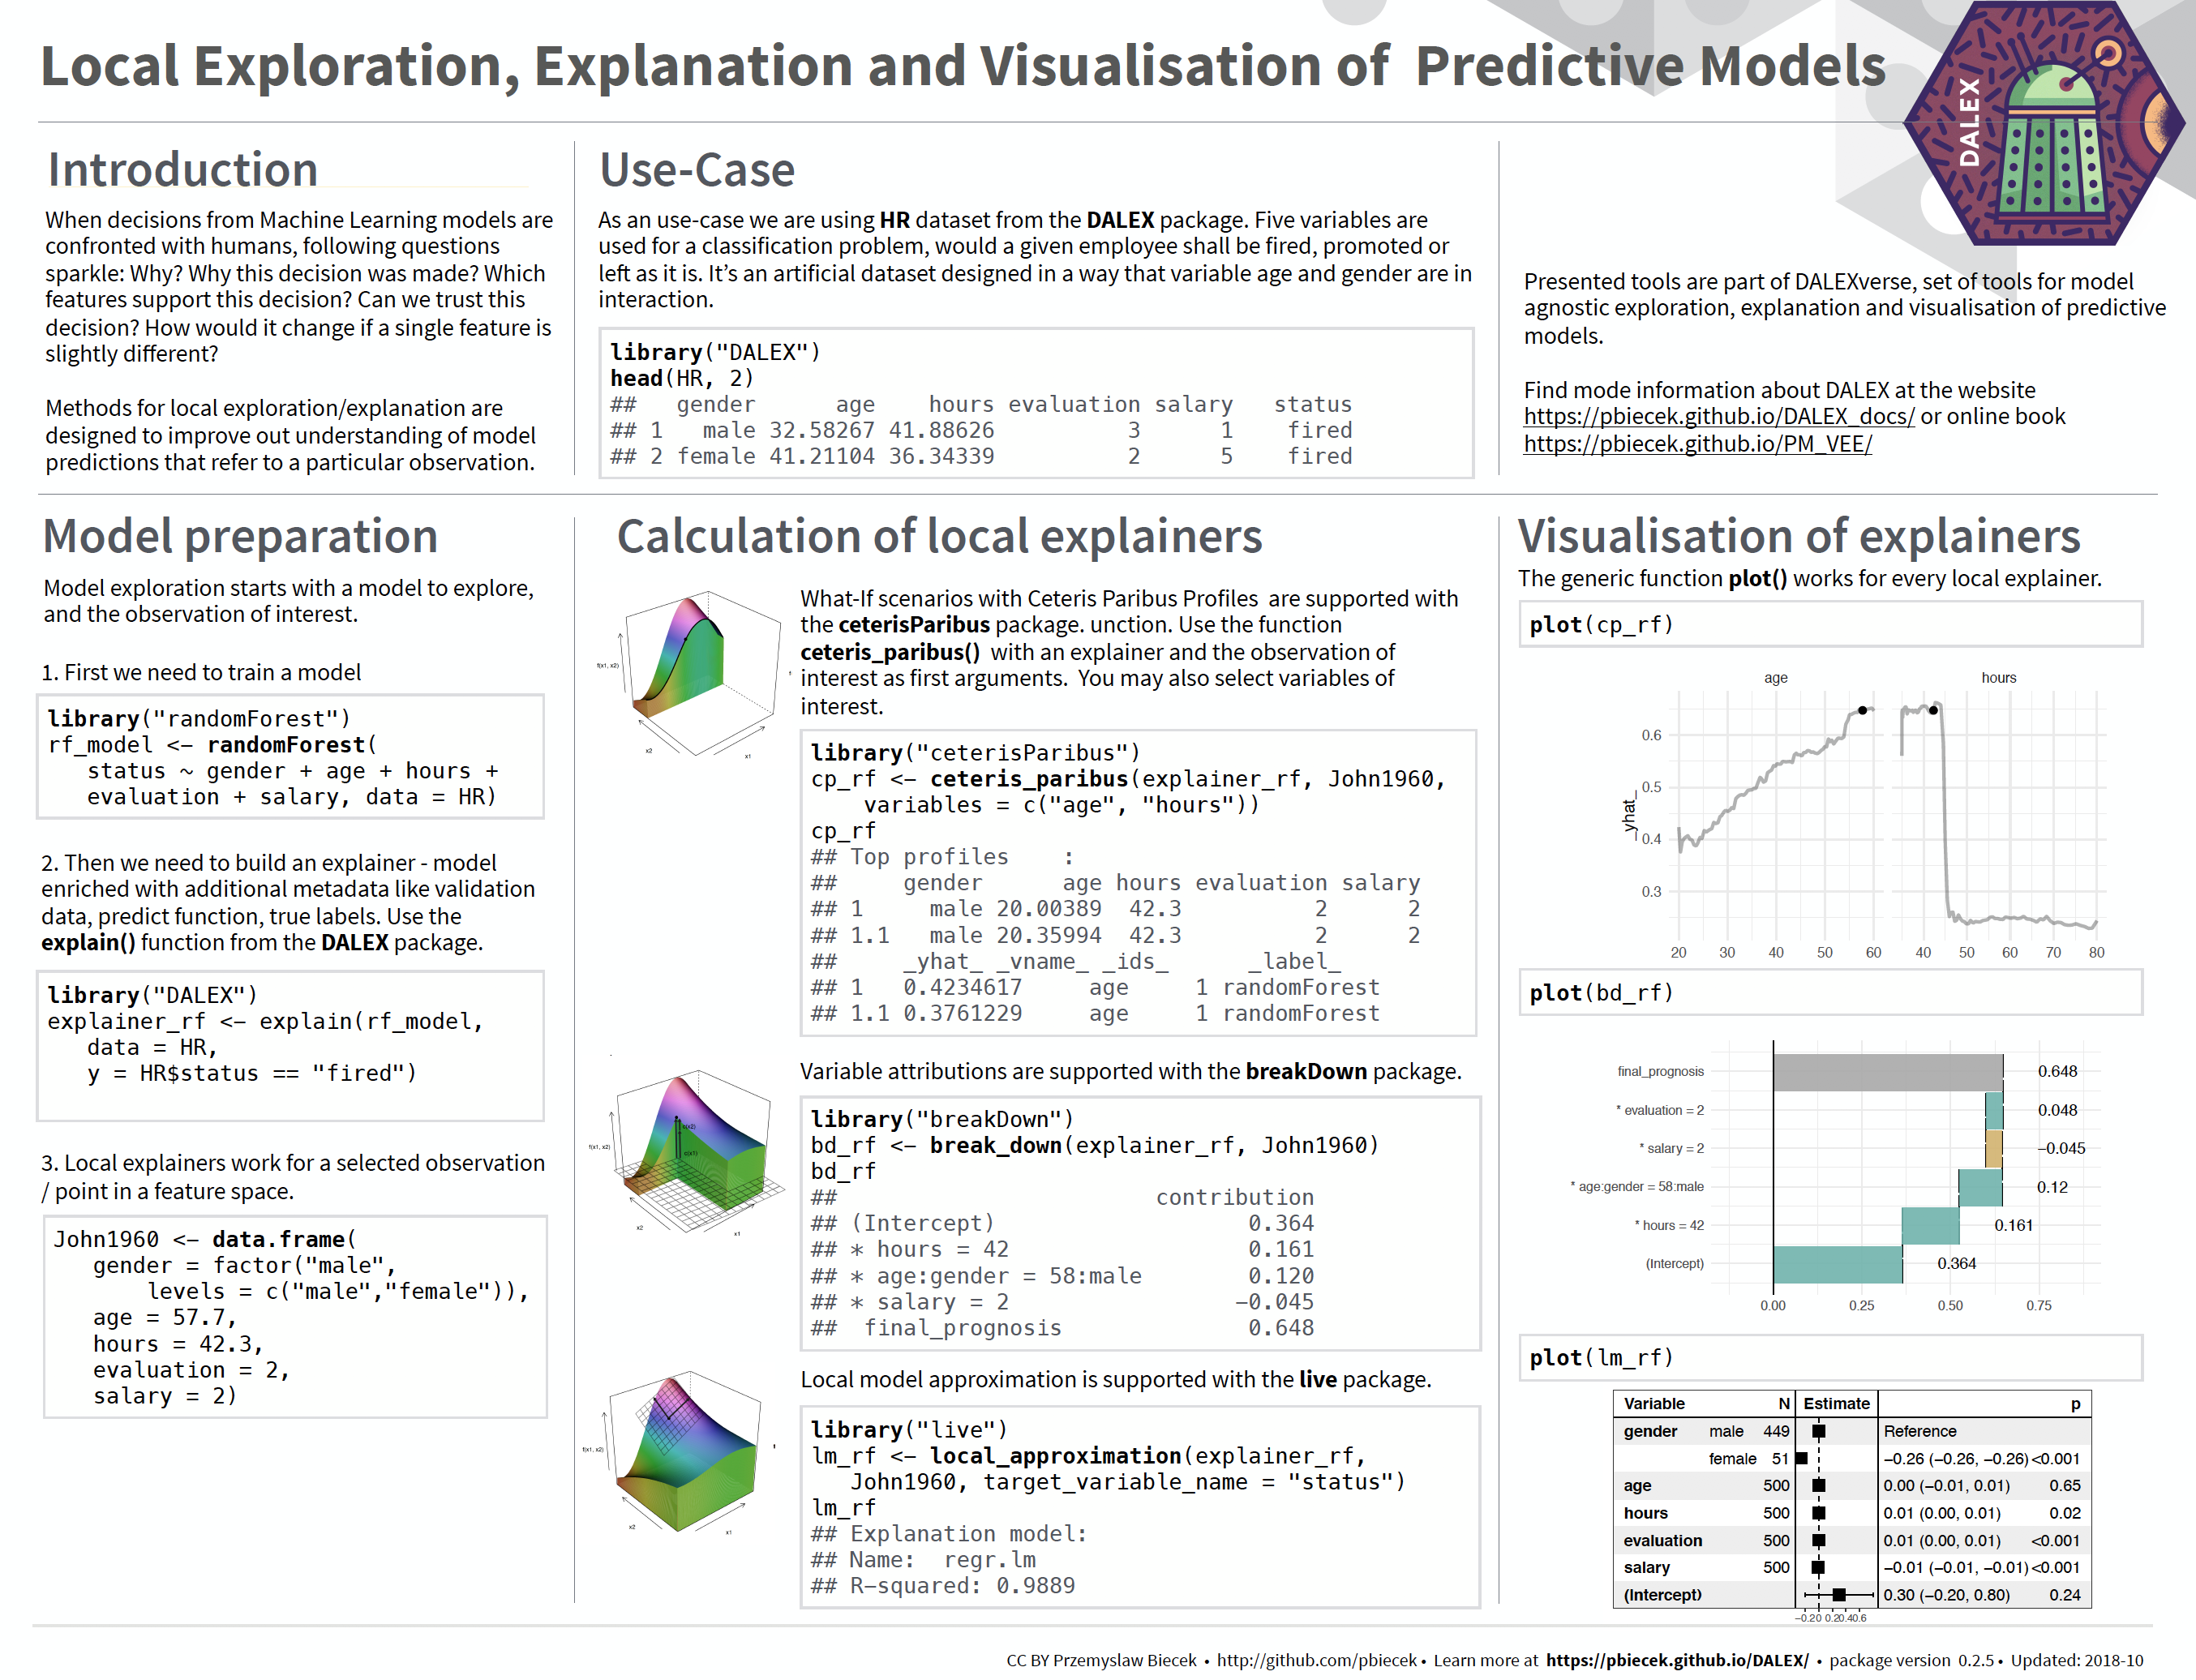
\includegraphics[width=0.99\linewidth]{figure/DALEX_local} 

}

\caption{(fig:localDALEXsummary) Summary of three approaches to local model exploration and explanation.}\label{fig:localDALEXsummary}
\end{figure}

Instance-level explainers help to understand how a model yields a
prediction for a single observation. We can think about the following
situations as examples:

\begin{itemize}
\tightlist
\item
  We may want to evaluate the effects of explanatory variables on model
  predictions. For instance, we may be interested in predicting the risk
  of heart attack based on person's age, sex, and smoking habits. A
  model may be used to construct a score (for instance, a linear
  combination of the explanatory variables representing age, sex, and
  smoking habits) that could be used for the purposes of prediction. For
  a particular patient we may want to learn how much the different
  variables contribute to the patient's score?
\item
  We may want to understand how models predictions would change if
  values of some of the explanatory variables changed. For instance,
  what would be the predicted risk of heart attack if the patient cut
  the number of cigarettes smoked per day by half?
\item
  We may discover that the model is providing incorrect predictions and
  we may want to find the reason. For instance, a patient with a very
  low risk-score experiences heart attack. What has driven that
  prediction?
\end{itemize}

A model is a function with a \(p\)-dimensional vector \(x\) as an
argument. The plot of the value(s) of the function can be constructed in
a \(p+1\)-dimensional space. An example with \(p=2\) is presented in
Figure \ref{fig:cutsSurfaceReady}. We will use it as an illustration of
key ideas. The plot provides an information about the values of the
function in the vicinity of point \(x^*\).

\begin{figure}

{\centering 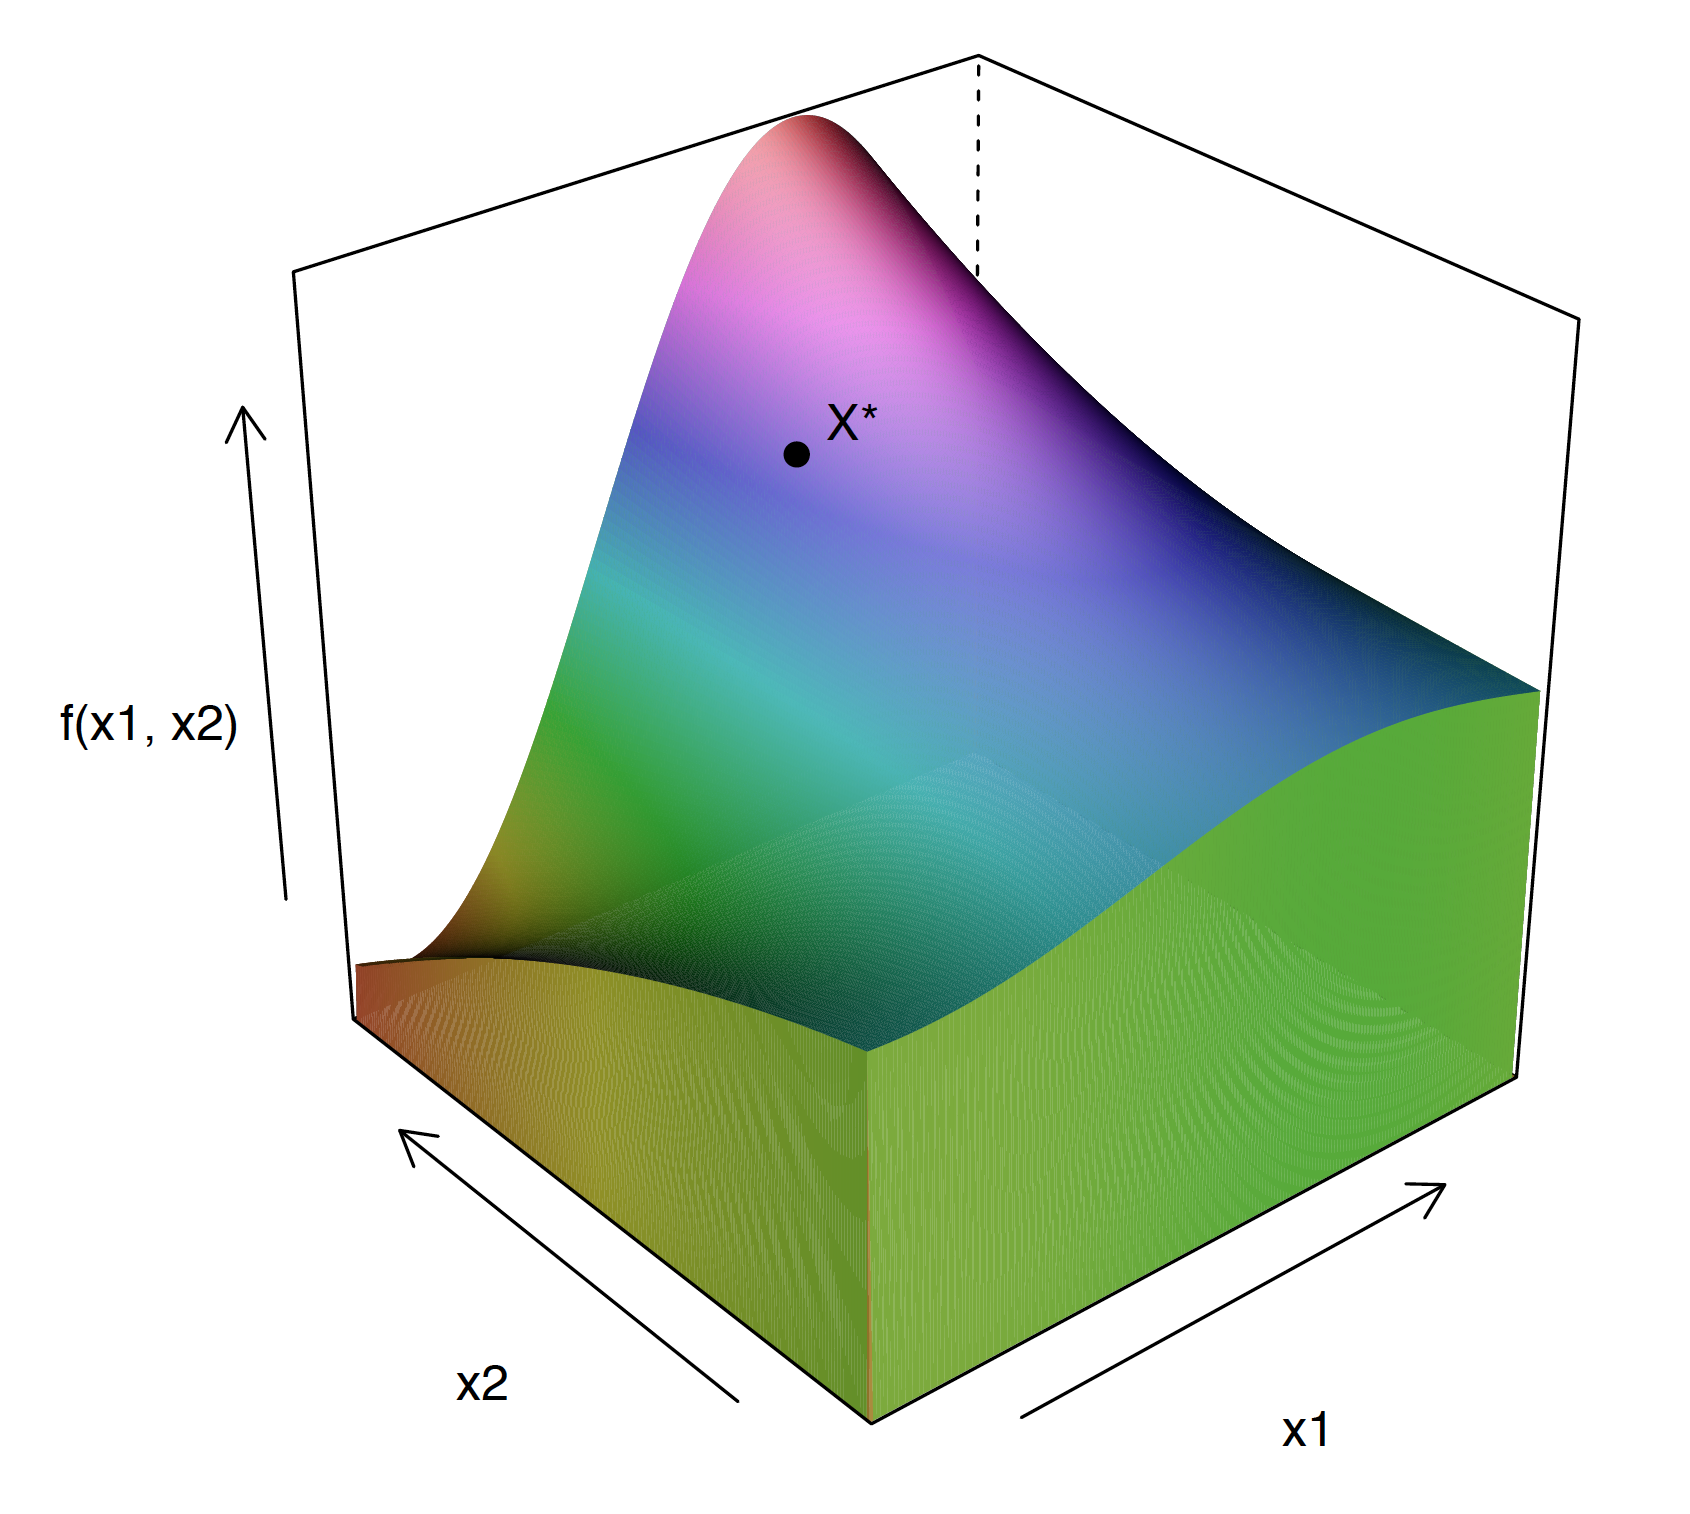
\includegraphics[width=0.6\linewidth]{figure/cuts_surface_ready_punkt} 

}

\caption{(fig:cutsSurfaceReady) Response surface for a model that is a function of two variables. We are interested in understanding the response of a model in a single point x*}\label{fig:cutsSurfaceReady}
\end{figure}

There are many different tools that may be used to explore the
predictions of the model around a single point \(x^*\). In the following
sections we will describe the most popular approaches. They can be
divided into three classes.

\begin{itemize}
\tightlist
\item
  One approach is to investigate how the model prediction changes if the
  value of a single explanatory variable changes. The approach is useful
  in the so-called ,,What-If'' analyses. In particular, we can construct
  plots presenting the change in model-based predictions induced by a
  change of a single variable. Such plots are usually called
  Ceteris-paribus (CP) profiles. An example is provided in panel A of
  Figure \ref{fig:cutsTechnikiReady}. Chapters
  \ref{ceterisParibus}-\ref{localDiagnostics} introduce the CP profiles
  and methods based on them.\\
\item
  Another approach is to analyze how the model prediction for point
  \(x^*\) is different from the average model prediction and how the
  difference can be distributed among explanatory variables. It is often
  called the ,,variable attributions'' approach. An example is provided
  in panel B of Figure \ref{fig:cutsTechnikiReady}. Chapters
  \ref{breakDown}-\ref{shapley} present various methods implementing
  this approach.
\item
  Yet another approach is to analyze the curvature of the response
  surface (see Figure \ref{fig:cutsSurfaceReady}) around the point of
  interest \(x^*\). Treating the model as a function, we are interested
  in the local behavior of this function around \(x^*\). In case of a
  black-box model, we may approximate it with a simpler glass-box model
  around \(x^*\). An example is provided in panel C of Figure
  \ref{fig:cutsTechnikiReady}. Chapter \ref{LIME} presents the Local
  Interpretable Model-agnostic Explanations (LIME) method that exploits
  the concept of a ,,local model.''
\end{itemize}

Each method has its own merits and limitations. They are briefly
discussed in the corresponding chapters. Chapter
\ref{SummaryInstanceLevel} offers a comparison of the methods.

\begin{figure}

{\centering 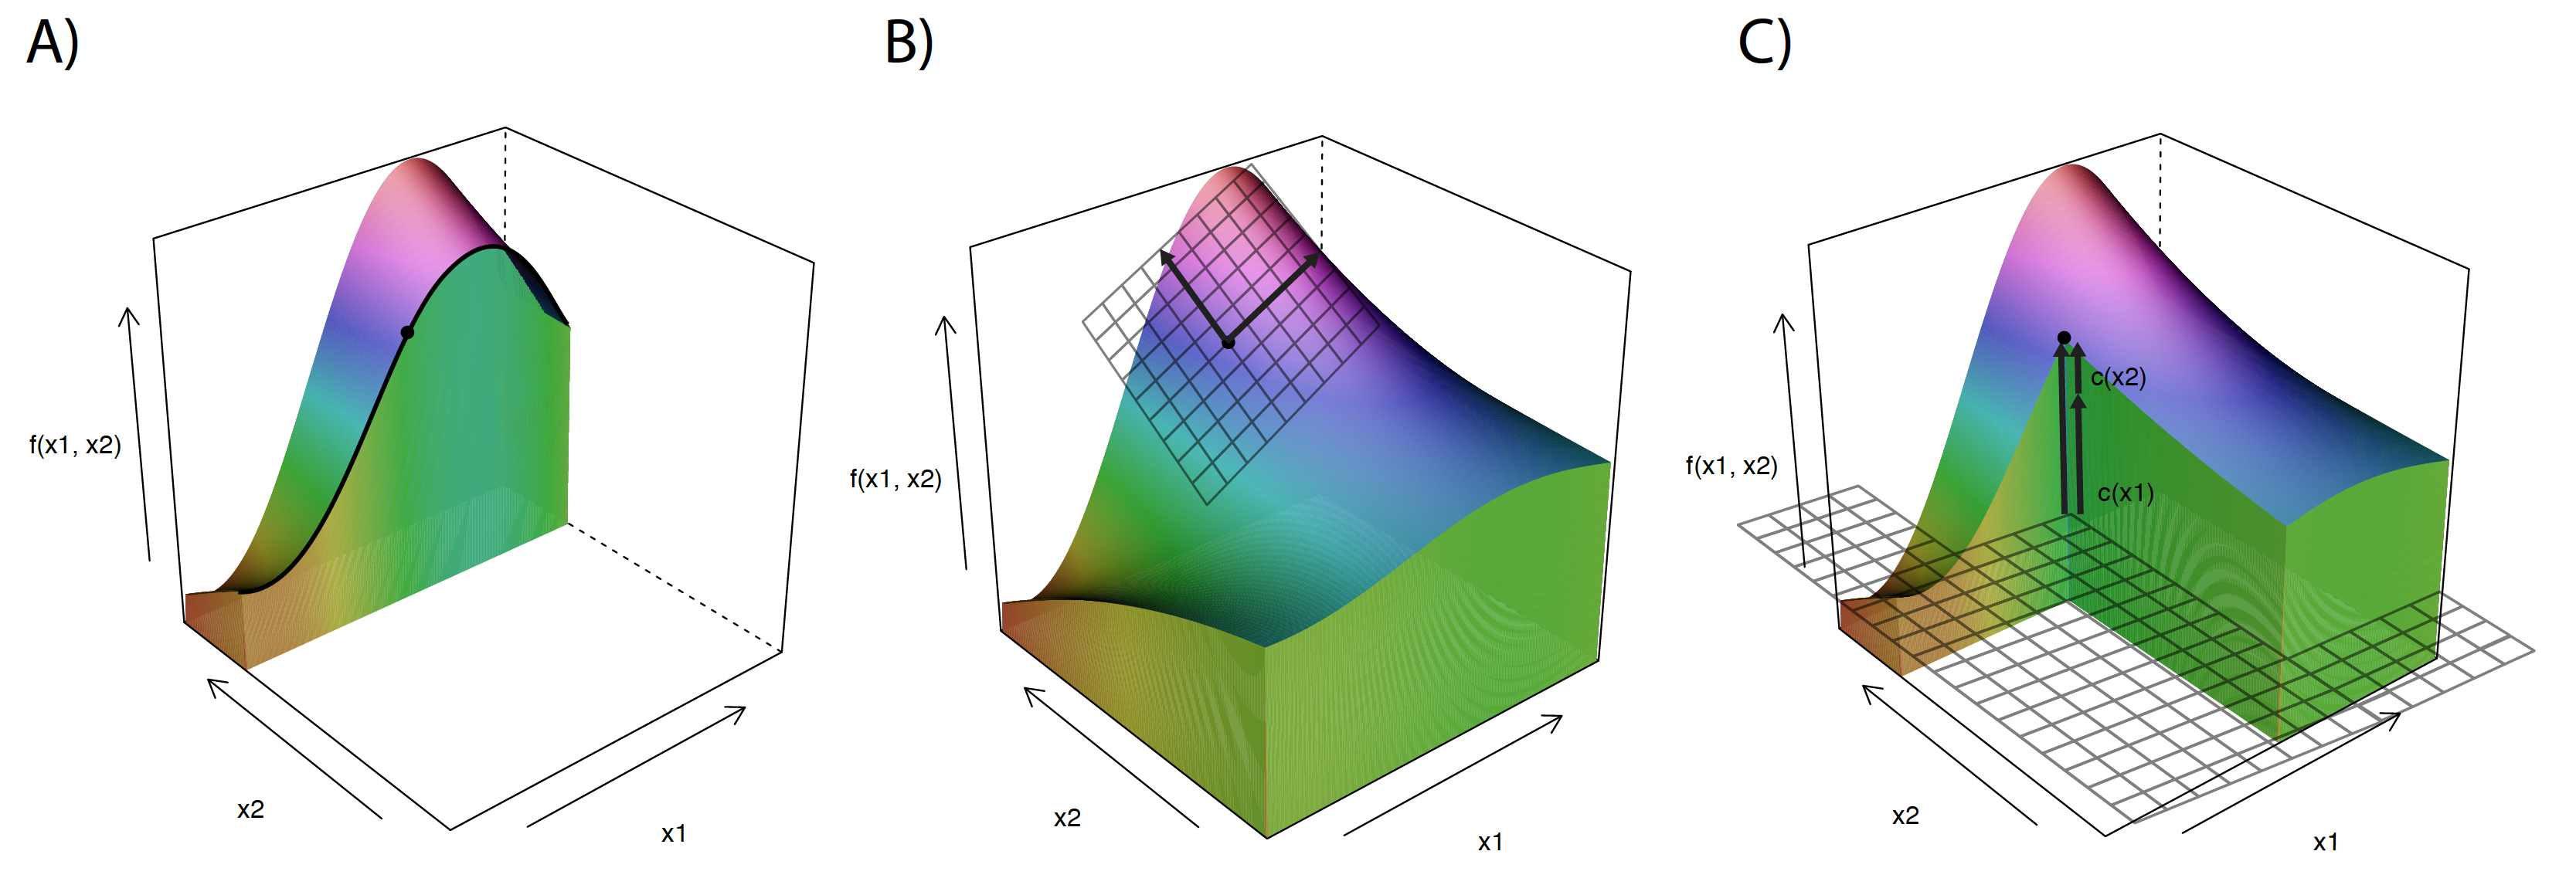
\includegraphics[width=0.99\linewidth]{figure/cuts_techniki_ready} 

}

\caption{(fig:cutsTechnikiReady) Illustration of different approaches to instance-level explanation. Panel A presents a What-If analysis with Ceteris-paribus profiles. The profiles show the model response as a function of a value of a single variable, while keeping the values of all other explanatory variables fixed. Panel B illustrates the concept of variable attributions. Additive effects of each variable show how the model response differs from the average. Panel C illustrates the concept of local models. A simpler glass-box model is fitted around the point of interest. It describes the local behaviour of the black-box model. }\label{fig:cutsTechnikiReady}
\end{figure}

\hypertarget{ceterisParibus}{%
\section{Ceteris-paribus Profiles and What-If
Analysis}\label{ceterisParibus}}

\hypertarget{CPIntro}{%
\subsection{Introduction}\label{CPIntro}}

\emph{Ceteris paribus} is a Latin phrase meaning ``other things held
constant'' or ``all else unchanged.'' In this chapter, we introduce a
technique for model exploration based on the \emph{Ceteris paribus}
principle. In particular, we examine the influence of each explanatory
variable, assuming that effects of all other variables are unchanged.
The main goal is to understand how changes in a single explanatory
variable affects model predictions.

Explanation tools (explainers) presented in this chapter are linked to
the second law introduced in Section \ref{three-single-laws}, i.e.~the
law of ``Prediction's speculation.'' This is why the tools are also
known as \emph{What-If model analysis} or \emph{Individual Conditional
Expectations} \citep{ICEbox}. It appears that it is easier to understand
how a black-box model is working if we can explore the model by
investigating the influence of explanatory variables separately,
changing one at a time.

\hypertarget{CPIntuition}{%
\subsection{Intuition}\label{CPIntuition}}

Panel A of Figure \ref{fig:modelResponseCurveLine} presents response
(prediction) surface for the \texttt{titanic\_lmr\_v6} model for two
explanatory variables, \emph{age} and \emph{class}, from the
\emph{titanic} dataset (see Section \ref{TitanicDataset}). We are
interested in the change of the model prediction induced by each of the
variables. Toward this end, we may want to explore the curvature of the
response surface around a single point with \emph{age} equal to 47 and
\emph{class} equal to ``1st,'' indicated in the plot. Ceteris-paribus
(CP) profiles are one-dimensional profiles that examine the curvature
across each dimension, i.e., for each variable. Panel B of Figure
\ref{fig:modelResponseCurveLine} presents the profiles corresponding to
\emph{age} and \emph{class}. Note that, in the CP profile for
\emph{age}, the point of interest is indicated by the black dot. In
essence, a CP profile shows a conditional expectation of the dependent
variable (response) for the particular explanatory variable.

\begin{figure}

{\centering 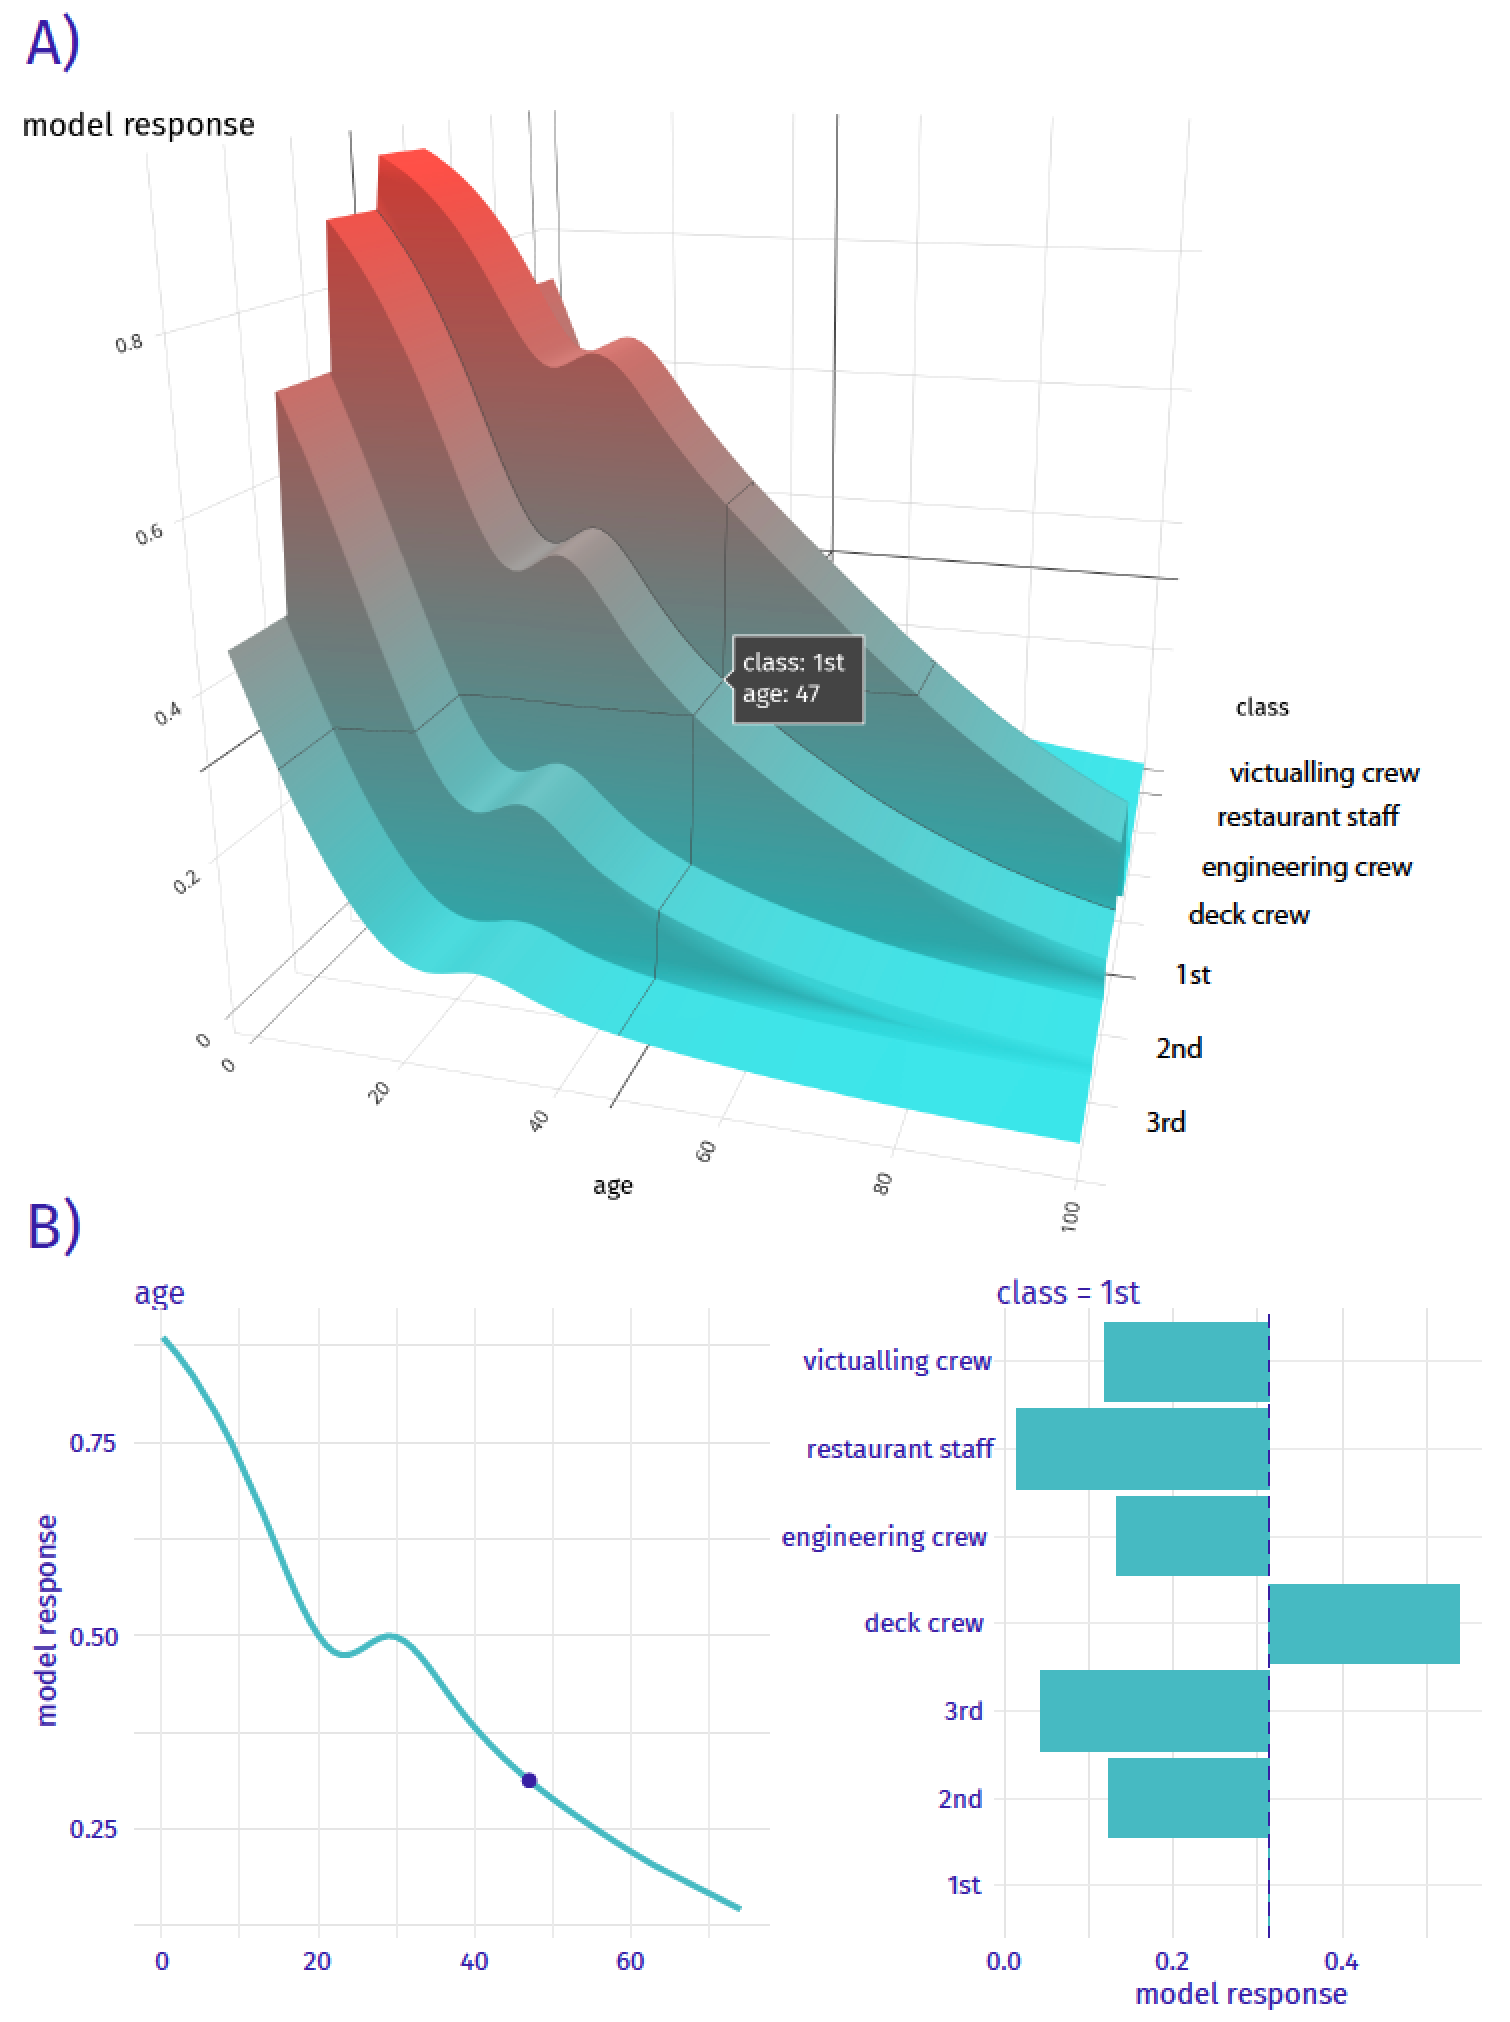
\includegraphics[width=0.7\linewidth]{figure/profile_age_class} 

}

\caption{(fig:modelResponseCurveLine) A) Model response (prediction) surface. Ceteris-paribus (CP) profiles marked with black curves help to understand the curvature of the surface while changing only a single explanatory variable. B) CP profiles for individual variables, age (continuous) and class (categorical).}\label{fig:modelResponseCurveLine}
\end{figure}

CP technique is similar to the LIME method (see Chapter \ref{LIME}).
LIME and CP profiles examine the curvature of response surface of a
model. The difference between these two methods lies in the fact that
LIME approximates the black-box model of interest locally with a simpler
glass-box model. Usually, the LIME model is sparse, i.e., contains fewer
explanatory variables. Thus, one needs to investigate a plot across a
smaller number of dimensions. On the other hand, the CP profiles present
conditional predictions for every variable and, in most cases, are
easier to interpret.

\hypertarget{CPMethod}{%
\subsection{Method}\label{CPMethod}}

In this section, we introduce more formally one-dimensional CP profiles.

In predictive modeling, we are interested in a distribution of a
dependent variable \(Y\) given vector \(x_*\). The latter contains
values of explanatory variables. In the ideal world, we would like to
know the conditional distribution of \(Y\) given \(x_*\). In practical
applications, however, we usually do not predict the entire
distribution, but just some of its characteristics like the expected
(mean) value, a quantile, or variance. Without loss of generality we
will assume that we model the conditional expected value
\(E_Y(Y | x_*)\).

Assume that we have got model \(f()\), for which \(f(x_*)\) is an
approximation of \(E_Y(Y | x_*)\), i.e.,
\(E_Y(Y | x_*) \approx f(x_*)\). Note that we do not assume that it is a
``good'' model, nor that the approximation is precise. We simply assume
that we have got a model that is used to estimate the conditional
expected value and to form predictions of the values of the dependent
variable. Our interest lies in the evaluation of the quality of the
predictions. If the model offers a ``good'' approximation of the
conditional expected value, it should be reflected in its satisfactory
predictive performance.

Recall (see Section \ref{notation}) that we use \(x_i\) to refer to the
vector corresponding to the \(i\)-th observation in a dataset. Let
\(x^{j}_{*}\) denote the \(j\)-th element of \(x_{*}\), i.e., the
\(j\)-th explanatory variable. We use \(x^{-j}_{*}\) to refer to a
vector resulting from removing the \(j\)-th element from \(x_{*}\). By
\(x^{j|=z}_{*}\), we denote a vector resulting from changing the value
of the \(j\)-th element of \(x_{*}\) to (a scalar) \(z\).

We define a one-dimensional CP profile \(h()\) for model \(f()\), the
\(j\)-th explanatory variable, and point \(x_*\) as follows:

\[
h^{f,j}_{x_*}(z) \equiv f(x_*^{j|=z}).
\] CP profile is a function that provides the dependence of the
approximated expected value (prediction) of \(Y\) on the value \(z\) of
the \(j\)-th explanatory variable. Note that, in practice, \(z\) is
taken to go through the entire range of values typical for the variable,
while values of all other explanatory variables are kept fixed at the
values specified by \(x_*\).

Note that in the situation when only a single model is considered, we
will skip the model index and we will denote the CP profile for the
\(j\)-th explanatory variable and the point of interest \(x_*\) by
\(h^{j}_{x_*}(z)\).

\hypertarget{CPExample}{%
\subsection{Example: Titanic}\label{CPExample}}

For continuous explanatory variables, a natural way to represent the CP
function is to use a profile plot similar to the ones presented in
Figure \ref{fig:profileAgeRf}. In the figure, the dot on the curves
marks an instance prediction, i.e., prediction \(f(x_*)\) for a single
observation \(x_*\). The curve itself shows how the prediction would
change if the value of a particular explanatory variable changed.

Figure \ref{fig:profileAgeRf} presents CP profiles for the \emph{age}
variable in the logistic regression and random forest models for the
Titanic dataset (see Sections \ref{model-titanic-lmr} and
\ref{model-titanic-rf}, respectively). It is worth observing that the
profile for the logistic regression model is smooth, while the one for
the random forest model shows more variability. For this instance
(observation), the prediction for the logistic regression model would
increase substantially if the value of \emph{age} became lower than 20.
For the random forrest model, a substantial increase would be obtained
if \emph{age} became lower than 13 or so.

\textbackslash{}begin\{figure\}

\{\centering 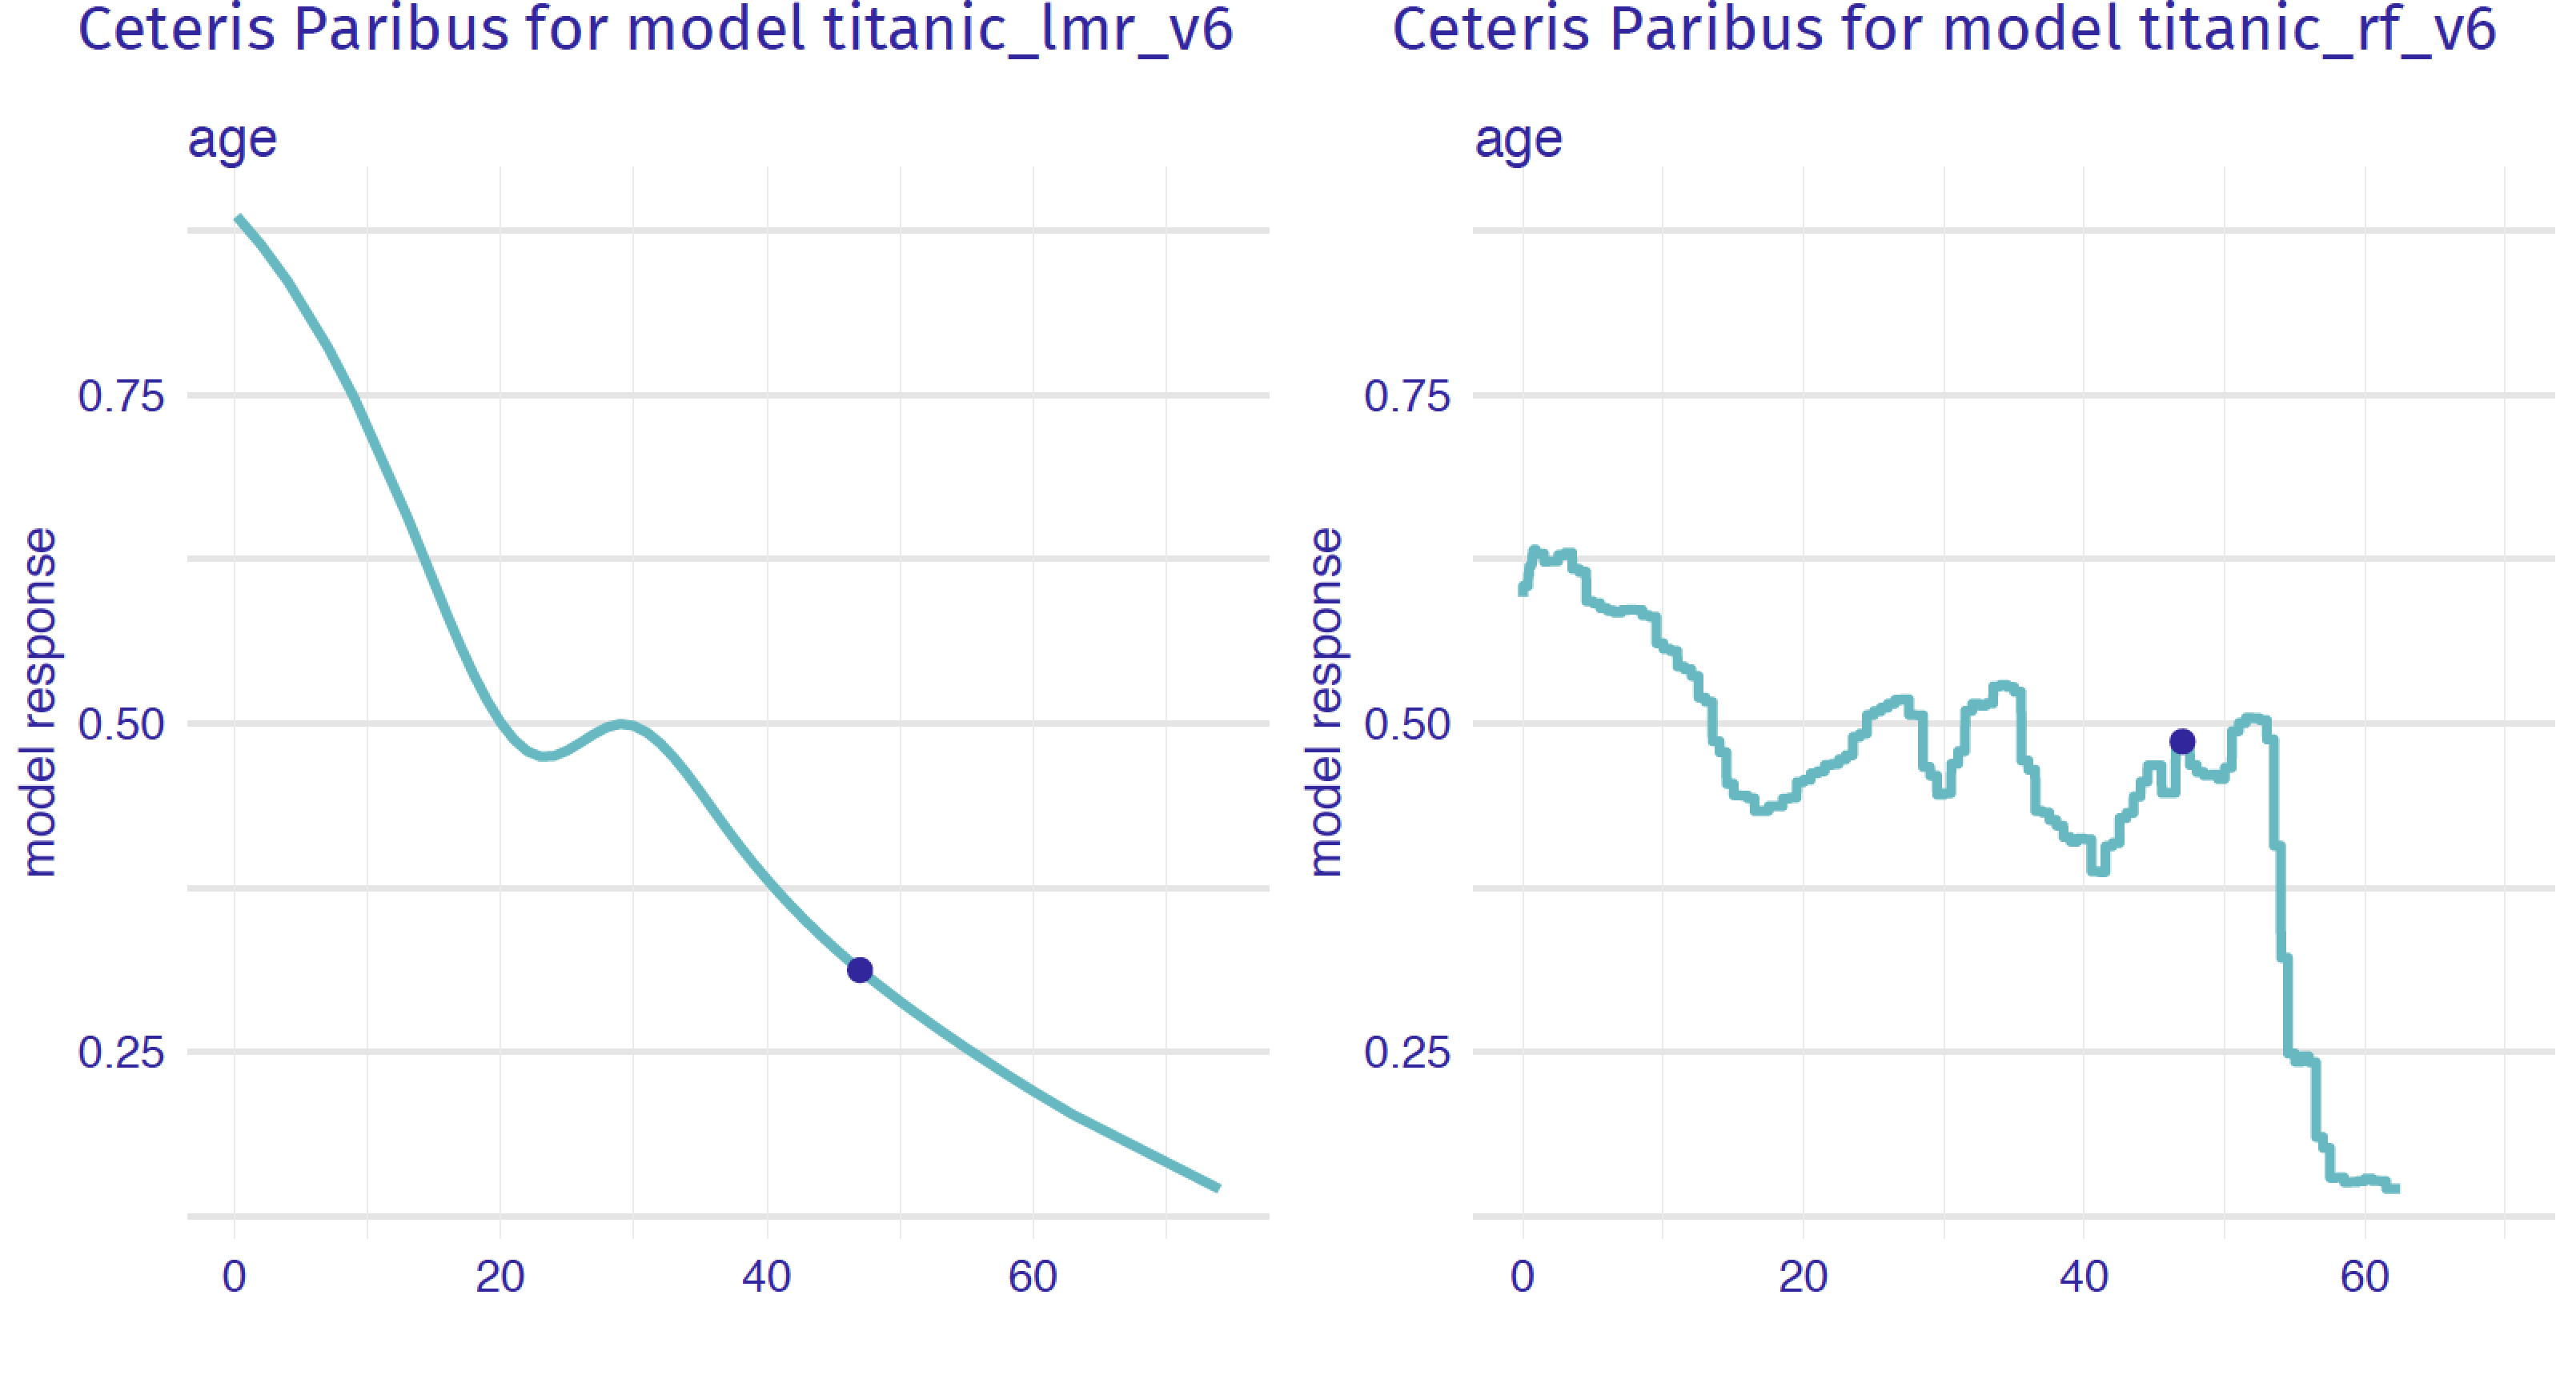
\includegraphics[width=0.7\linewidth]{figure/profile_age_rf}

\}

\textbackslash{}caption\{(fig:profileAgeRf) Ceteris-paribus profiles for
variable \texttt{age} for the logistic regression
(\texttt{titanic\_lmr\_v6}) and random forest (\texttt{titanic\_rf\_v6}
) models that predict the probability of surviving based on the Titanic
data\}\label{fig:profileAgeRf} \textbackslash{}end\{figure\}

For a categorical explanatory variable, a natural way to represent the
CP function is to use a barplot similar to the ones presented in Figure
\ref{fig:profileAgeRf2}. The barplots in Figure \ref{fig:profileAgeRf}
present CP profiles for the \emph{class} variable in the logistic
regression and random forest models for the Titanic dataset (see
Sections \ref{model-titanic-lmr} and \ref{model-titanic-rf},
respectively). For this instance (observation), the predicted
probability for the logistic regression model would decrease
substantially if the value of \emph{class} changed to ``2nd''. On the
other hand, for the random forest model, the largest change would be
marked if \emph{class} changed to ``restaurant staff''.

\textbackslash{}begin\{figure\}

\{\centering 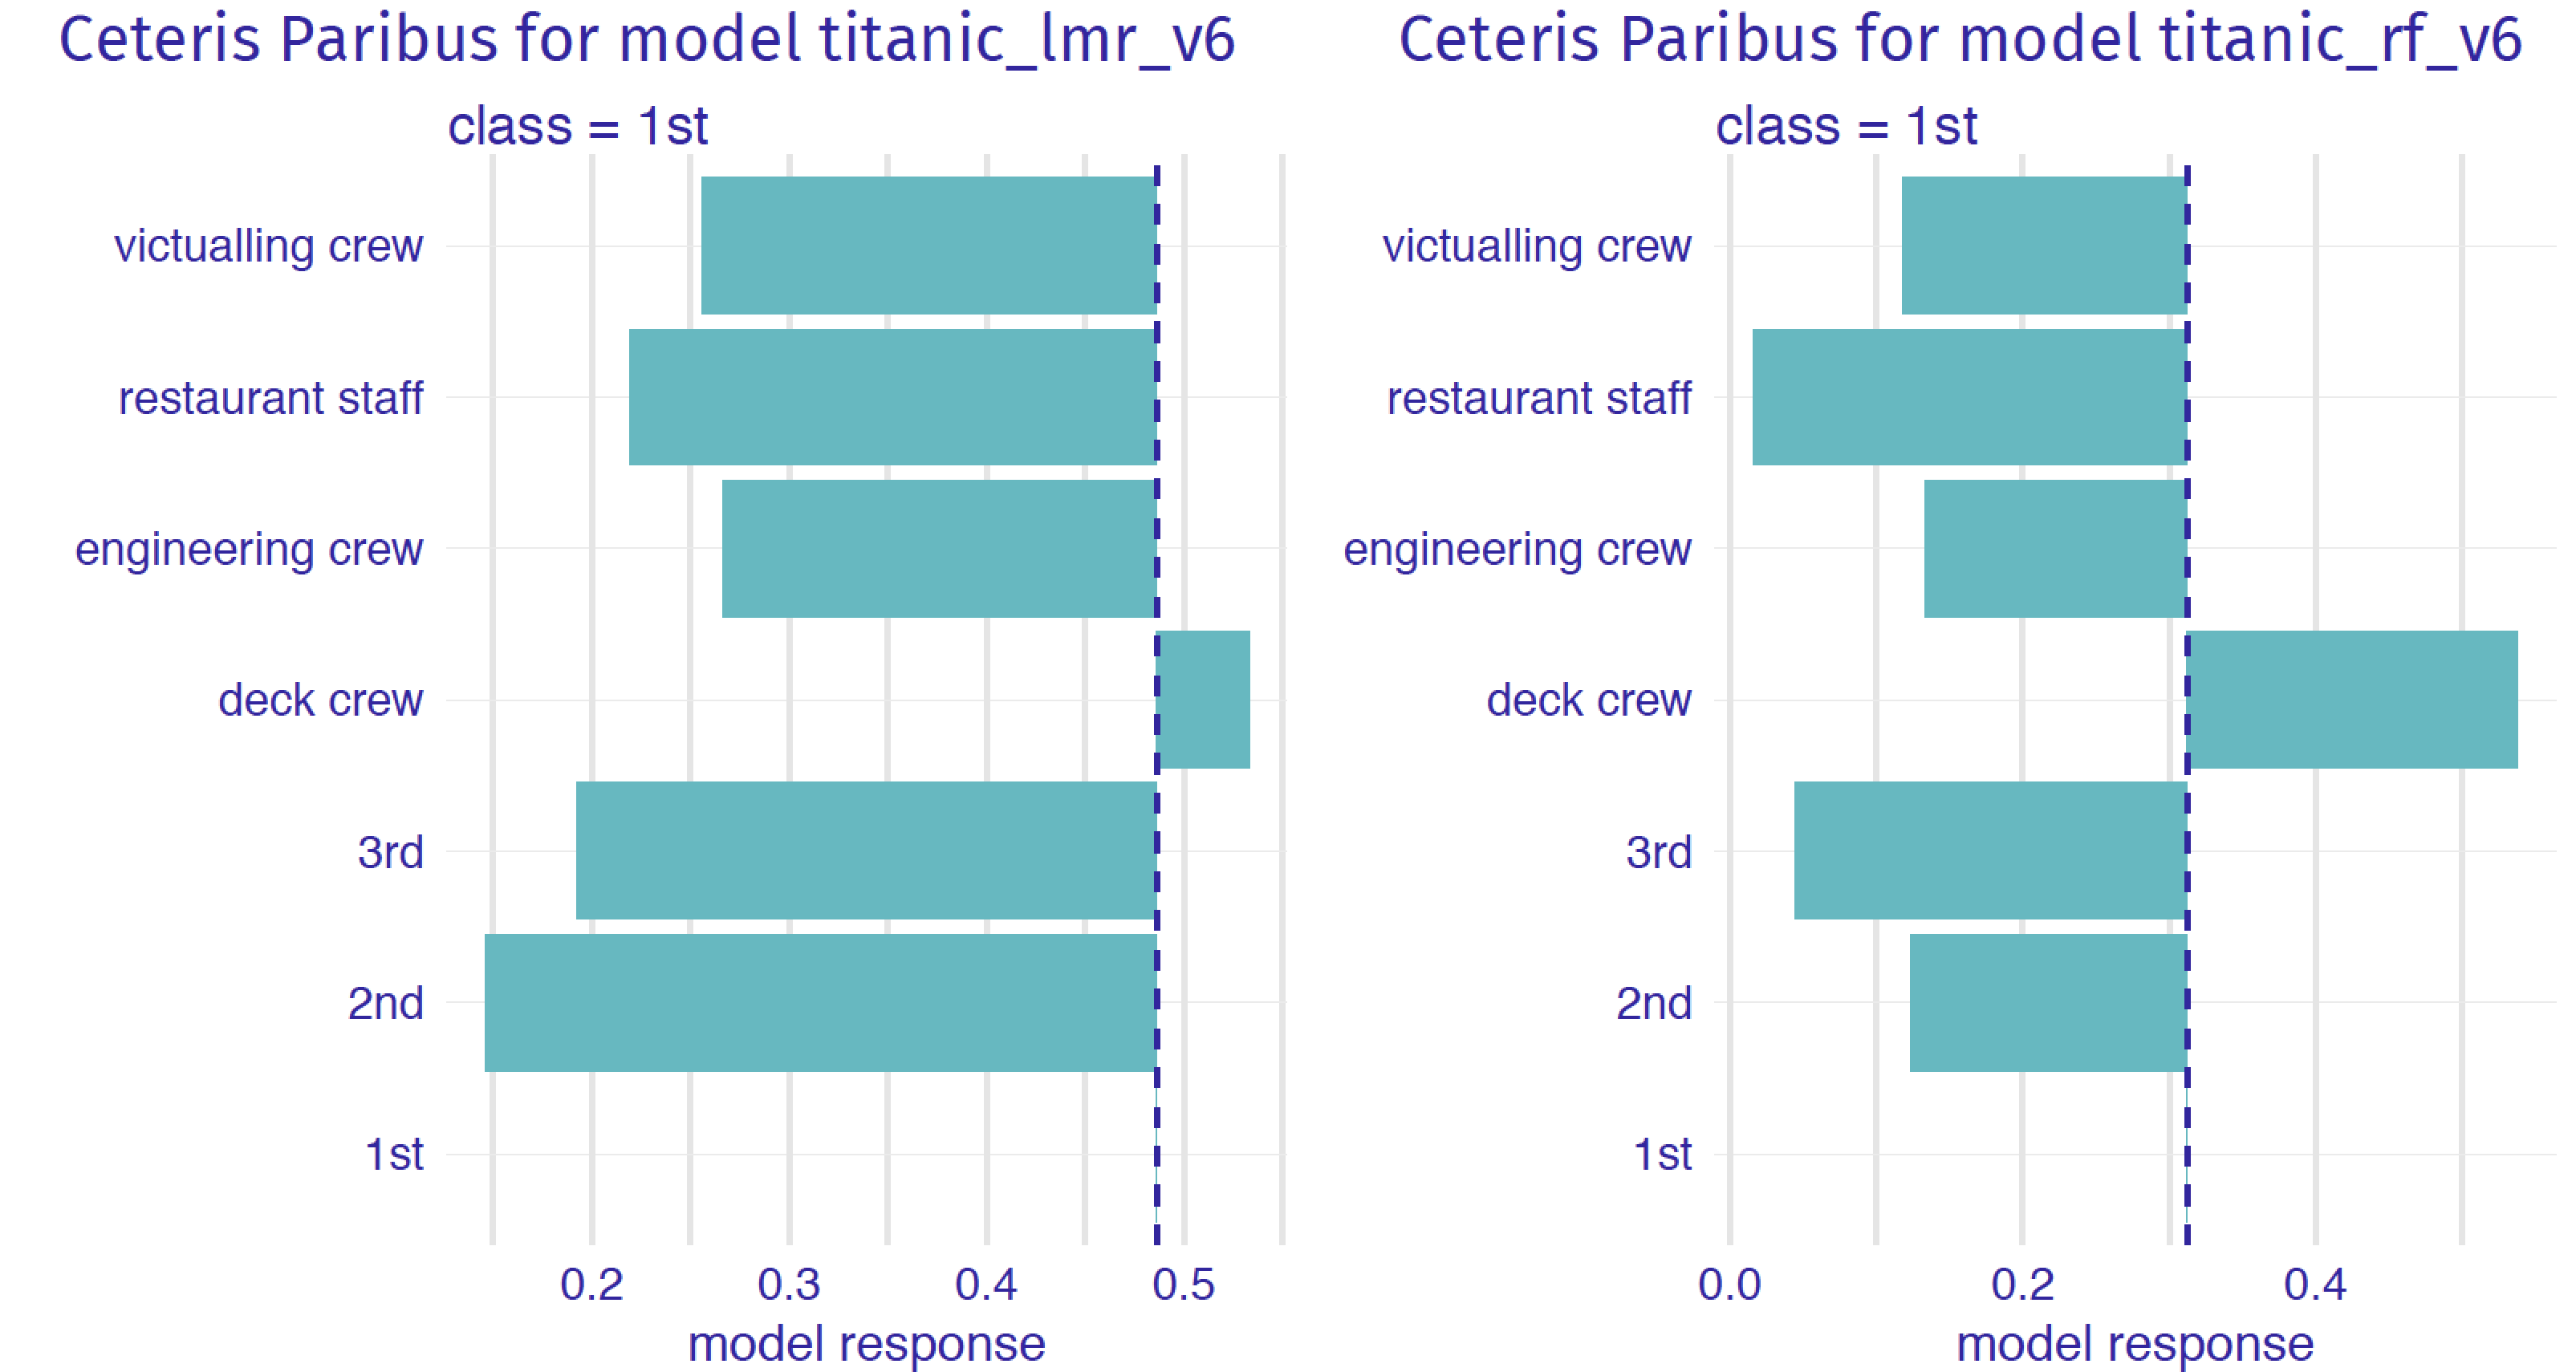
\includegraphics[width=0.7\linewidth]{figure/profile_class_rf}

\}

\textbackslash{}caption\{(fig:profileAgeRf2) Ceteris-paribus profiles
for variable \texttt{class} for the logistic regression
(\texttt{titanic\_lmr\_v6}) and random forest (\texttt{titanic\_rf\_v6}
) models that predict the probability of surviving based on the Titanic
data\}\label{fig:profileAgeRf2} \textbackslash{}end\{figure\}

Usually, black-box models contain a large number of explanatory
variables. However, CP profiles are legible even for tiny subplots,
created with techniques like sparklines or small multiples
\citep{Tufte1986}. In this way we can display a large number of profiles
at the same time keeping profiles for consecutive variables in separate
panels, as shown in Figure \ref{fig:profileV4Rf} for the random forest
model for the Titanic dataset. It helps if these panels are ordered so
that the most important profiles are listed first. We discuss a method
to assess the importance of CP profiles in the next chapter.

\textbackslash{}begin\{figure\}

\{\centering 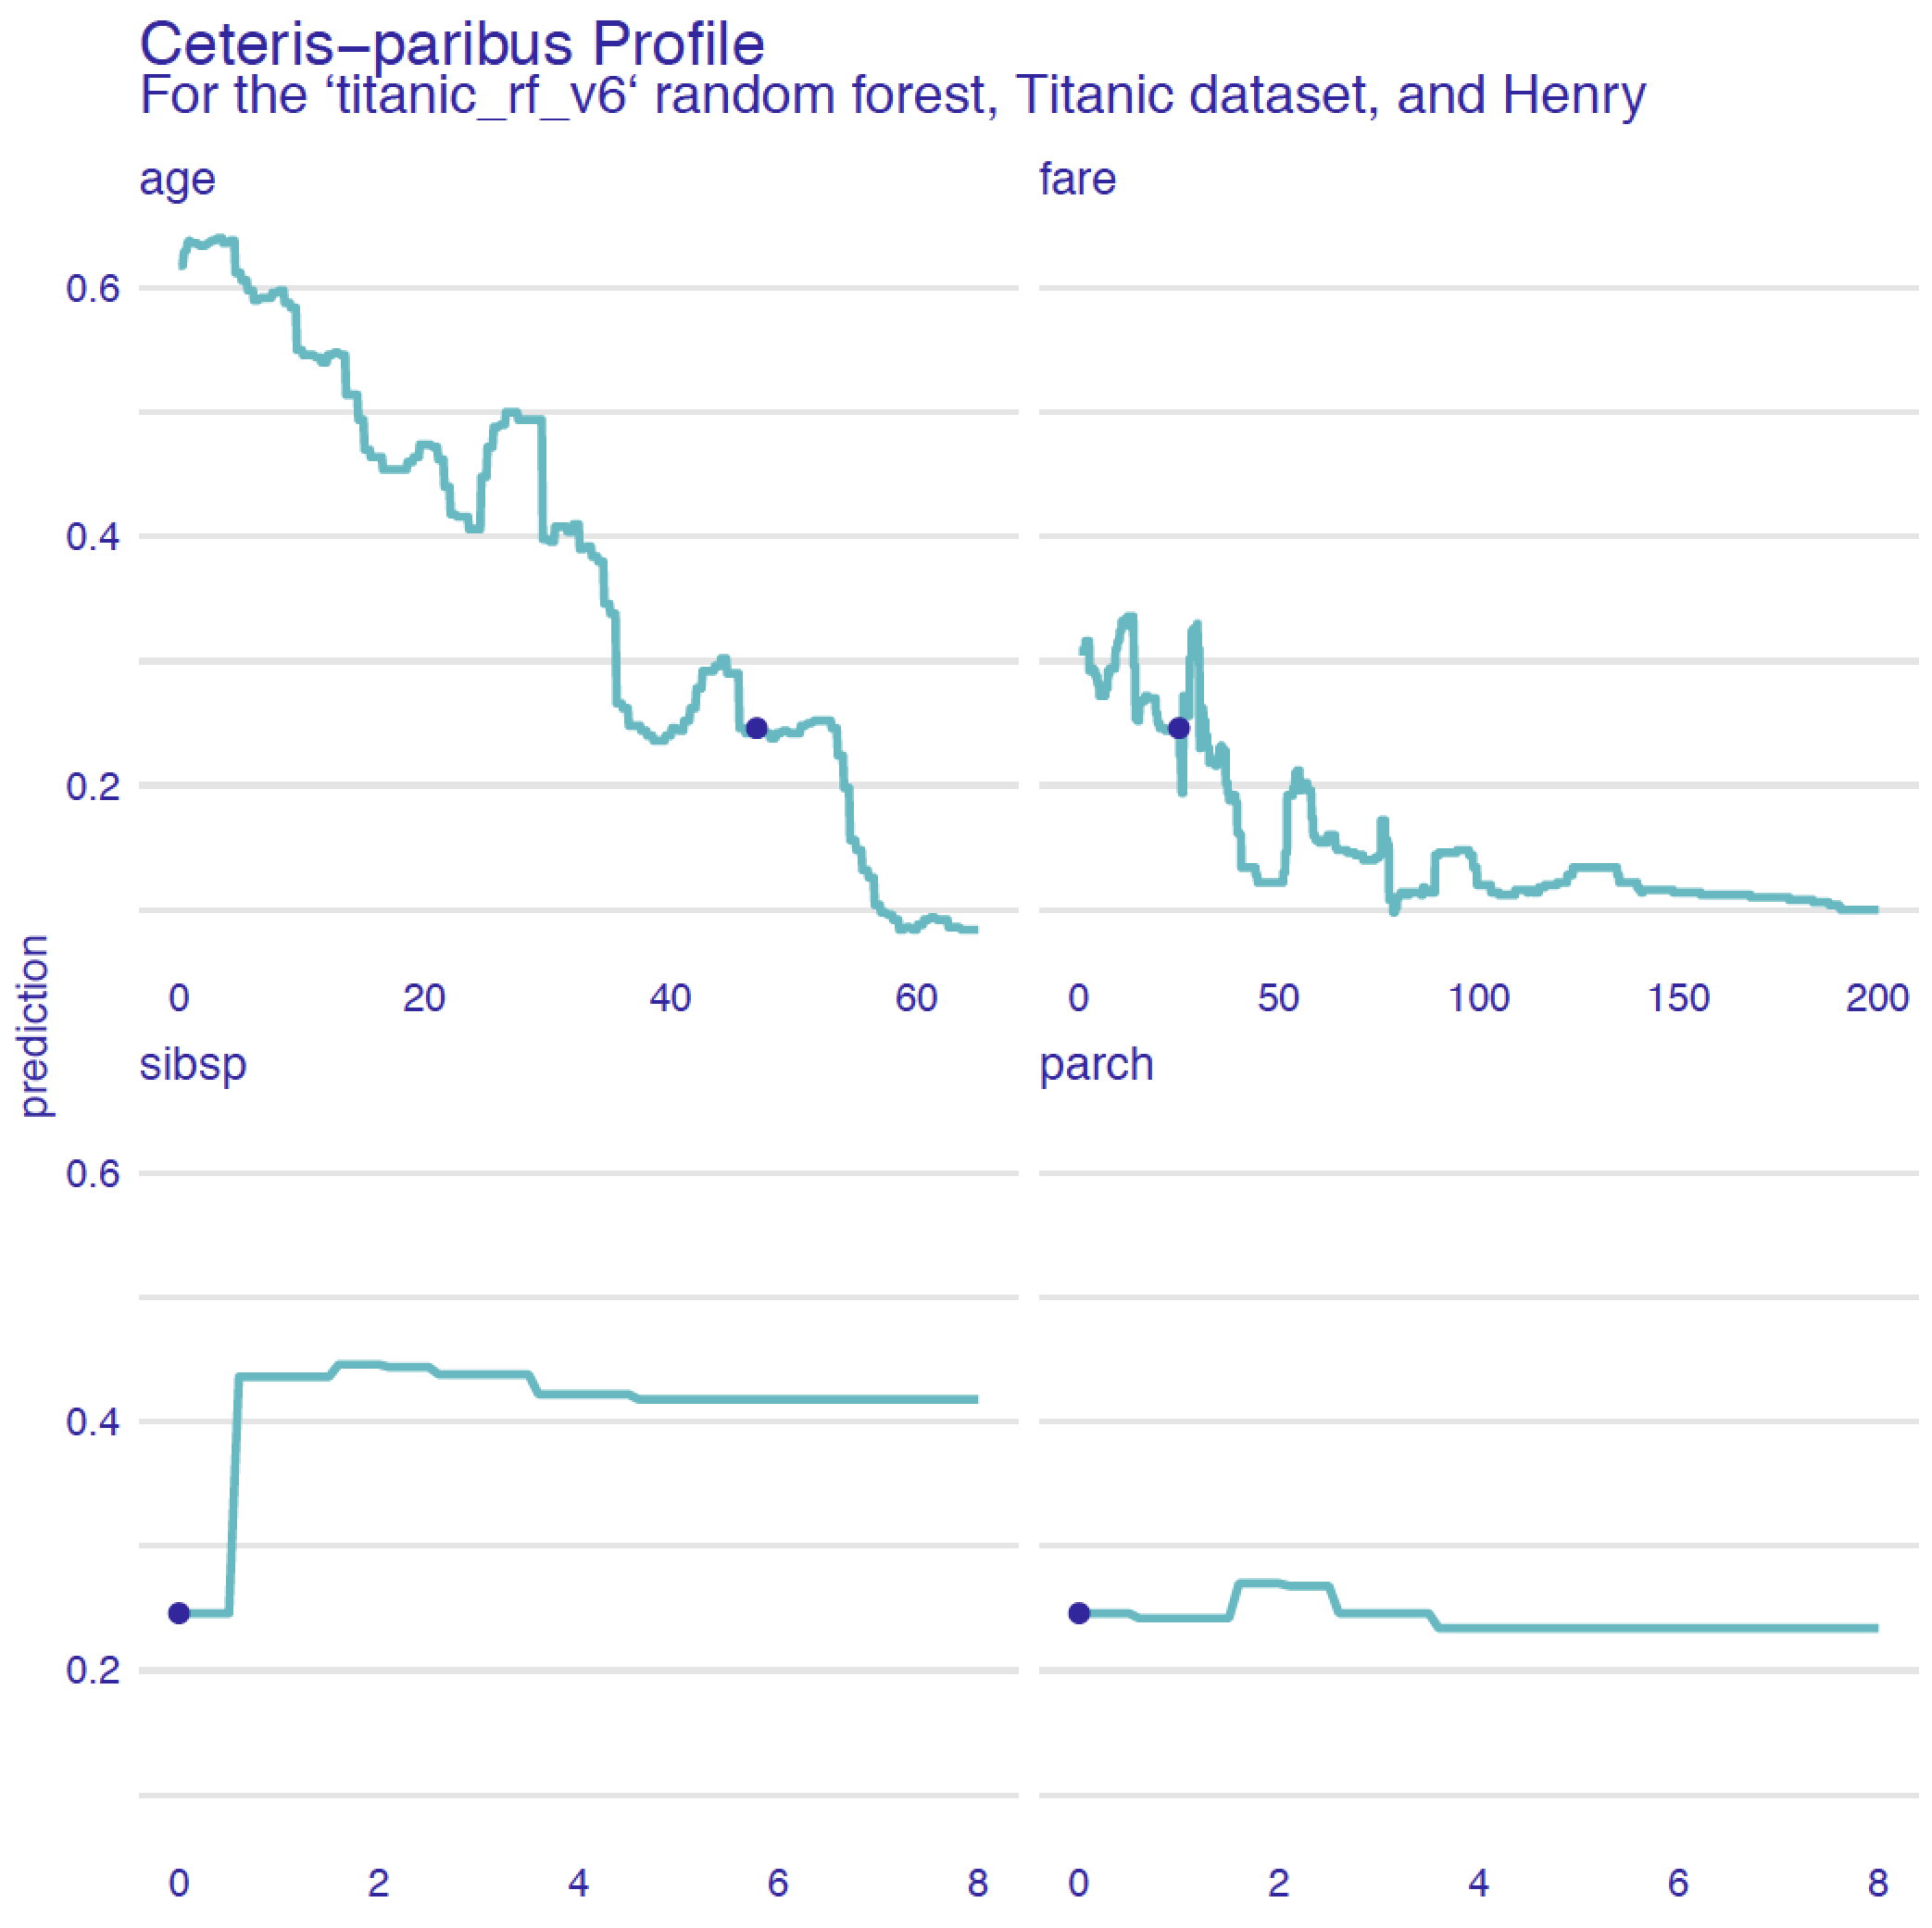
\includegraphics[width=0.7\linewidth]{figure/profile_v4_rf3}

\}

\textbackslash{}caption\{(fig:profileV4Rf) Ceteris-paribus profiles for
all continuous explanatory variables for the random forest
(\texttt{titanic\_rf\_v6}) model for the \texttt{titanic}
dataset\}\label{fig:profileV4Rf} \textbackslash{}end\{figure\}

\hypertarget{CPProsCons}{%
\subsection{Pros and cons}\label{CPProsCons}}

One-dimensional CP profiles, as presented in this chapter, offer a
uniform, easy to communicate and extendable approach to model
exploration. Their graphical representation is easy to understand and
explain. It is possible to show profiles for many variables or models in
a single plot. CP profiles are easy to compare, thus we can juxtapose
two or more models to better understand differences between models. We
can also compare two or more instances to better understand model
stability. CP profiles are also a useful tool for sensitivity analysis.

There are several issues related to the use of the CP profiles. If
explanatory variables are correlated, then changing one variable implies
a change in the other. In such case, the application of the
\emph{Ceteris paribus} principle may lead to unrealistic settings, as it
is not possible to keep one variable fixed while varying the other one.
For example, apartment's price prediction features like surface and
number of rooms are correlated thus it is unrealistic to consider very
small apartments with extreme number of rooms. Special cases are
interactions, which require the use of two-dimensional CP profiles that
are more complex than one-dimensional ones. Also, in case of a model
with hundreds or thousands of variables, the number of plots to inspect
may be daunting. Finally, while barplots allow visualization of CP
profiles for factors (categorical explanatory variables), their use
becomes less trivial in case of factors with many nominal (unordered)
categories (like, for example, a ZIP-code).

\hypertarget{CPR}{%
\subsection{Code snippets for R}\label{CPR}}

In this section, we present key features of the R package
\texttt{ingredients} \citep{ingredientsRPackage} which is a part of
\texttt{DrWhy.AI} universe and covers all methods presented in this
chapter. More details and examples can be found at
\url{https://modeloriented.github.io/ingredients/}.

Note that there are also other R packages that offer similar
functionality, like \texttt{condvis} \citep{JSSv081i05}, \texttt{pdp}
\citep{pdpRPackage}, \texttt{ICEbox} \citep{ICEboxRPackage},
\texttt{ALEPlot} \citep{ALEPlotRPackage}, \texttt{iml}
\citep{imlRPackage}.

For illustration, we use two classification models developed in Chapter
\ref{TitanicDataset}, namely the logistic regression model
\texttt{titanic\_lmr\_v6} (Section \ref{model-titanic-lmr}) and the
random forest model \texttt{titanic\_rf\_v6} (Section
\ref{model-titanic-rf}). They are developed to predict the probability
of survival after sinking of Titanic. Instance-level explanations are
calculated for a single observation \texttt{henry} - a 47 years old male
passenger that travelled in the 1st class.

\texttt{DALEX} explainers for both models and the \texttt{henry} data
frame are retrieved via the \texttt{archivist} hooks as listed in
Section \ref{ListOfModelsTitanic}.

\begin{Shaded}
\begin{Highlighting}[]
\KeywordTok{library}\NormalTok{(}\StringTok{"rms"}\NormalTok{)}
\NormalTok{explain_lmr_v6 <-}\StringTok{ }\NormalTok{archivist}\OperatorTok{::}\KeywordTok{aread}\NormalTok{(}\StringTok{"pbiecek/models/2b9b6"}\NormalTok{)}

\KeywordTok{library}\NormalTok{(}\StringTok{"randomForest"}\NormalTok{)}
\NormalTok{explain_rf_v6 <-}\StringTok{ }\NormalTok{archivist}\OperatorTok{::}\KeywordTok{aread}\NormalTok{(}\StringTok{"pbiecek/models/9b971"}\NormalTok{)}

\KeywordTok{library}\NormalTok{(}\StringTok{"DALEX"}\NormalTok{)}
\NormalTok{henry <-}\StringTok{ }\NormalTok{archivist}\OperatorTok{::}\KeywordTok{aread}\NormalTok{(}\StringTok{"pbiecek/models/a6538"}\NormalTok{)}
\NormalTok{henry}
\end{Highlighting}
\end{Shaded}

\begin{verbatim}
##   class gender age sibsp parch fare  embarked
## 1   1st   male  47     0     0   25 Cherbourg
\end{verbatim}

\hypertarget{basic-use-of-the-ceteris_paribus-function}{%
\subsubsection{\texorpdfstring{Basic use of the
\texttt{ceteris\_paribus}
function}{Basic use of the ceteris\_paribus function}}\label{basic-use-of-the-ceteris_paribus-function}}

The easiest way to create and plot CP profiles is to call
\texttt{ceteris\_paribus()} function and then the generic
\texttt{plot()} function. By default, profiles for all variables are
being calculated and all numeric features are being plotted. One can
limit the number of variables that should be considered with the
\texttt{variables} argument.

To obtain CP profiles, the \texttt{ceteris\_paribus()} function requires
the explainer-object and the instance data frame as arguments. As a
result, the function yields an object od the class
\texttt{ceteris\_paribus\_explainer}. It is a data frame with model
predictions.

\begin{Shaded}
\begin{Highlighting}[]
\KeywordTok{library}\NormalTok{(}\StringTok{"ingredients"}\NormalTok{)}
\NormalTok{cp_titanic_rf <-}\StringTok{ }\KeywordTok{ceteris_paribus}\NormalTok{(explain_rf_v6, henry)}
\NormalTok{cp_titanic_rf}
\end{Highlighting}
\end{Shaded}

\begin{verbatim}
## Top profiles    : 
##                class gender age sibsp parch fare  embarked _yhat_ _vname_
## 1                3rd   male  47     0     0   25 Cherbourg  0.100   class
## 1.1              2nd   male  47     0     0   25 Cherbourg  0.054   class
## 1.2              1st   male  47     0     0   25 Cherbourg  0.246   class
## 1.3 engineering crew   male  47     0     0   25 Cherbourg  0.096   class
## 1.4 victualling crew   male  47     0     0   25 Cherbourg  0.098   class
## 1.5 restaurant staff   male  47     0     0   25 Cherbourg  0.092   class
##     _ids_          _label_
## 1       1 Random Forest v6
## 1.1     1 Random Forest v6
## 1.2     1 Random Forest v6
## 1.3     1 Random Forest v6
## 1.4     1 Random Forest v6
## 1.5     1 Random Forest v6
## 
## 
## Top observations:
##   class gender age sibsp parch fare  embarked _yhat_          _label_
## 1   1st   male  47     0     0   25 Cherbourg  0.246 Random Forest v6
##   _ids_
## 1     1
\end{verbatim}

To obtain a graphical representation of CP profiles, the generic
\texttt{plot()} function can be applied to the data frame returned by
the \texttt{ceteris\_paribus()} function. It returns a \texttt{ggplot2}
object that can be processed further if needed. In the examples below,
we use the \texttt{ggplot2} functions, like \texttt{ggtitle()} or
\texttt{ylim()}, to modify plot's title or the range of the Y-axis.

The resulting plot can be enriched with additional data by applying
functions \texttt{ingredients::show\_rugs()} (adds rugs for the selected
points), \texttt{ingredients::show\_observations} (adds dots that shows
observations), or \texttt{ingredients::show\_aggreagated\_profiles}. All
these functions can take additional arguments to modify size, color, or
linetype.

Below we show an R snippet that can be used to replicate plots presented
in the upper part of Figure \ref{fig:profileV4Rf}.

\begin{Shaded}
\begin{Highlighting}[]
\KeywordTok{library}\NormalTok{(}\StringTok{"ggplot2"}\NormalTok{)}
\KeywordTok{plot}\NormalTok{(cp_titanic_rf, }\DataTypeTok{variables =} \KeywordTok{c}\NormalTok{(}\StringTok{"age"}\NormalTok{, }\StringTok{"fare"}\NormalTok{)) }\OperatorTok{+}
\StringTok{  }\KeywordTok{show_observations}\NormalTok{(cp_titanic_rf, }\DataTypeTok{variables =} \KeywordTok{c}\NormalTok{(}\StringTok{"age"}\NormalTok{, }\StringTok{"fare"}\NormalTok{)) }\OperatorTok{+}
\StringTok{  }\KeywordTok{ggtitle}\NormalTok{(}\StringTok{"Ceteris Paribus Profiles"}\NormalTok{, }\StringTok{"For the random forest model and the Titanic dataset"}\NormalTok{)}
\end{Highlighting}
\end{Shaded}

\textbackslash{}begin\{figure\}

\{\centering 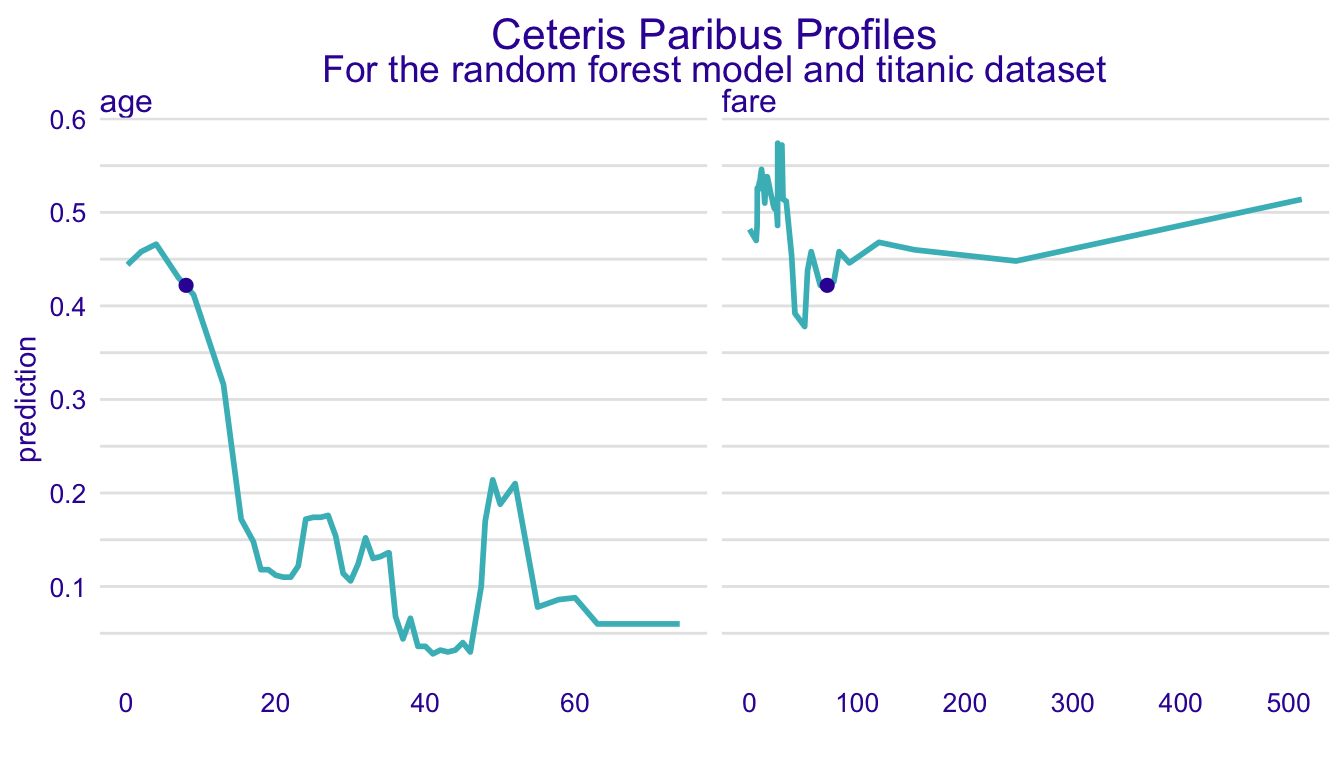
\includegraphics[width=0.7\linewidth]{PM_VEE_files/figure-latex/titanicCeterisProfile01-1}

\}

\textbackslash{}caption\{Ceteris-paribus profiles for \texttt{age} and
\texttt{fare} variables and the \texttt{titanic\_rf\_v6}
model.\}\label{fig:titanicCeterisProfile01} \textbackslash{}end\{figure\}

By default, all numerical variables are plotted. To plot CP profiles for
categorical variables, we have got to add the
\texttt{only\_numerical\ =\ FALSE} argument to the \texttt{plot()}
function. The code below an be used to recreate the right-hand-side plot
from Figure \ref{fig:profileAgeRf2}.

\begin{Shaded}
\begin{Highlighting}[]
\KeywordTok{plot}\NormalTok{(cp_titanic_rf, }\DataTypeTok{variables =} \KeywordTok{c}\NormalTok{(}\StringTok{"class"}\NormalTok{, }\StringTok{"embarked"}\NormalTok{), }\DataTypeTok{only_numerical =} \OtherTok{FALSE}\NormalTok{) }\OperatorTok{+}
\StringTok{  }\KeywordTok{ggtitle}\NormalTok{(}\StringTok{"Ceteris Paribus Profiles"}\NormalTok{, }\StringTok{"For the random forest model and the Titanic dataset"}\NormalTok{)}
\end{Highlighting}
\end{Shaded}

\textbackslash{}begin\{figure\}

\{\centering 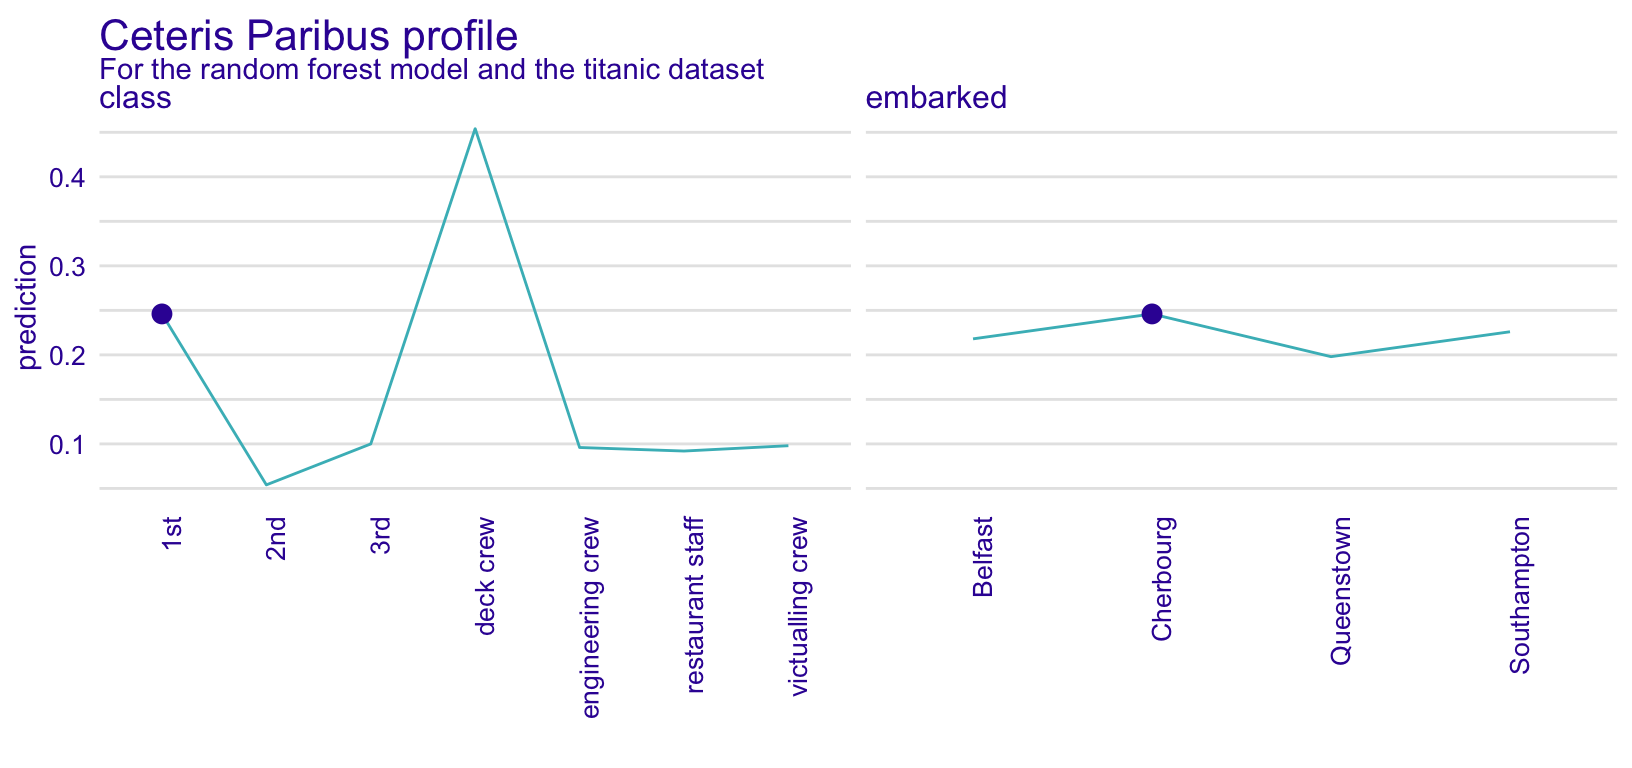
\includegraphics[width=0.7\linewidth]{PM_VEE_files/figure-latex/titanicCeterisProfile01B-1}

\}

\textbackslash{}caption\{Ceteris-paribus profiles for \texttt{class} and
\texttt{embarked} variables and the \texttt{titanic\_rf\_v6}
model.\}\label{fig:titanicCeterisProfile01B} \textbackslash{}end\{figure\}

\hypertarget{advanced-use-of-the-ceteris_paribus-function}{%
\subsubsection{\texorpdfstring{Advanced use of the
\texttt{ceteris\_paribus}
function}{Advanced use of the ceteris\_paribus function}}\label{advanced-use-of-the-ceteris_paribus-function}}

The \texttt{ceteris\_paribus()} is a very flexible function. To better
understand how it can be used, we briefly review its arguments.

\begin{itemize}
\tightlist
\item
  \texttt{x}, \texttt{data}, \texttt{predict\_function}, \texttt{label}
  - information about a model. If \texttt{x} is created with the
  \texttt{DALEX::explain} function, then other arguments are extracted
  from \texttt{x}; this is how we use the function in this chapter.
  Otherwise, we have got to specify directly the model, the validation
  data, the predict function, and the model label.
\item
  \texttt{new\_observation} - instance (one or more), for which we want
  to calculate CP profiles. It should be a data frame with same
  variables as in the validation data.
\item
  \texttt{y} - observed value of the dependent variable for
  \texttt{new\_observation}. The use of this argument is illustrated in
  Section \ref{cPLocDiagIntro}.
\item
  \texttt{variables} - names of explanatory variables, for which CP
  profiles are to be calculated. By default, the profiles will be
  constructed for all variables, which may be time consuming.
\item
  \texttt{variable\_splits} - a list of values for which CP profiles are
  to be calculated. By default, these are all values for categorical
  variables. For continuous variables, uniformly-placed values are
  selected; one can specify the number of the values with the
  \texttt{grid\_points} argument (the default is 101).
\end{itemize}

The code below allows to obtain the plots in the upper part of Figure
\ref{fig:profileV4Rf}. The argument \texttt{variable\_splits} specifies
the variables (\texttt{age} and \texttt{fare}) for which CP profiles are
to be calculated, together with the list of values at which the profiles
are to be evaluated.

\begin{Shaded}
\begin{Highlighting}[]
\NormalTok{cp_titanic_rf <-}\StringTok{ }\KeywordTok{ceteris_paribus}\NormalTok{(explain_rf_v6, henry,}
              \DataTypeTok{variable_splits =} \KeywordTok{list}\NormalTok{(}\DataTypeTok{age =} \KeywordTok{seq}\NormalTok{(}\DecValTok{0}\NormalTok{, }\DecValTok{70}\NormalTok{, }\FloatTok{0.1}\NormalTok{),}
                                     \DataTypeTok{fare =} \KeywordTok{seq}\NormalTok{(}\DecValTok{0}\NormalTok{, }\DecValTok{100}\NormalTok{, }\FloatTok{0.1}\NormalTok{)))}
\end{Highlighting}
\end{Shaded}

\begin{Shaded}
\begin{Highlighting}[]
\KeywordTok{plot}\NormalTok{(cp_titanic_rf) }\OperatorTok{+}\StringTok{ }
\StringTok{  }\KeywordTok{show_observations}\NormalTok{(cp_titanic_rf, }\DataTypeTok{variables =} \KeywordTok{c}\NormalTok{(}\StringTok{"age"}\NormalTok{, }\StringTok{"fare"}\NormalTok{), }\DataTypeTok{size =} \DecValTok{5}\NormalTok{) }\OperatorTok{+}\StringTok{ }
\StringTok{  }\KeywordTok{ylim}\NormalTok{(}\DecValTok{0}\NormalTok{, }\DecValTok{1}\NormalTok{) }\OperatorTok{+}
\StringTok{  }\KeywordTok{ggtitle}\NormalTok{(}\StringTok{"Ceteris Paribus Profiles"}\NormalTok{, }\StringTok{"For the random forest model and titanic dataset"}\NormalTok{)}
\end{Highlighting}
\end{Shaded}

\textbackslash{}begin\{figure\}

\{\centering 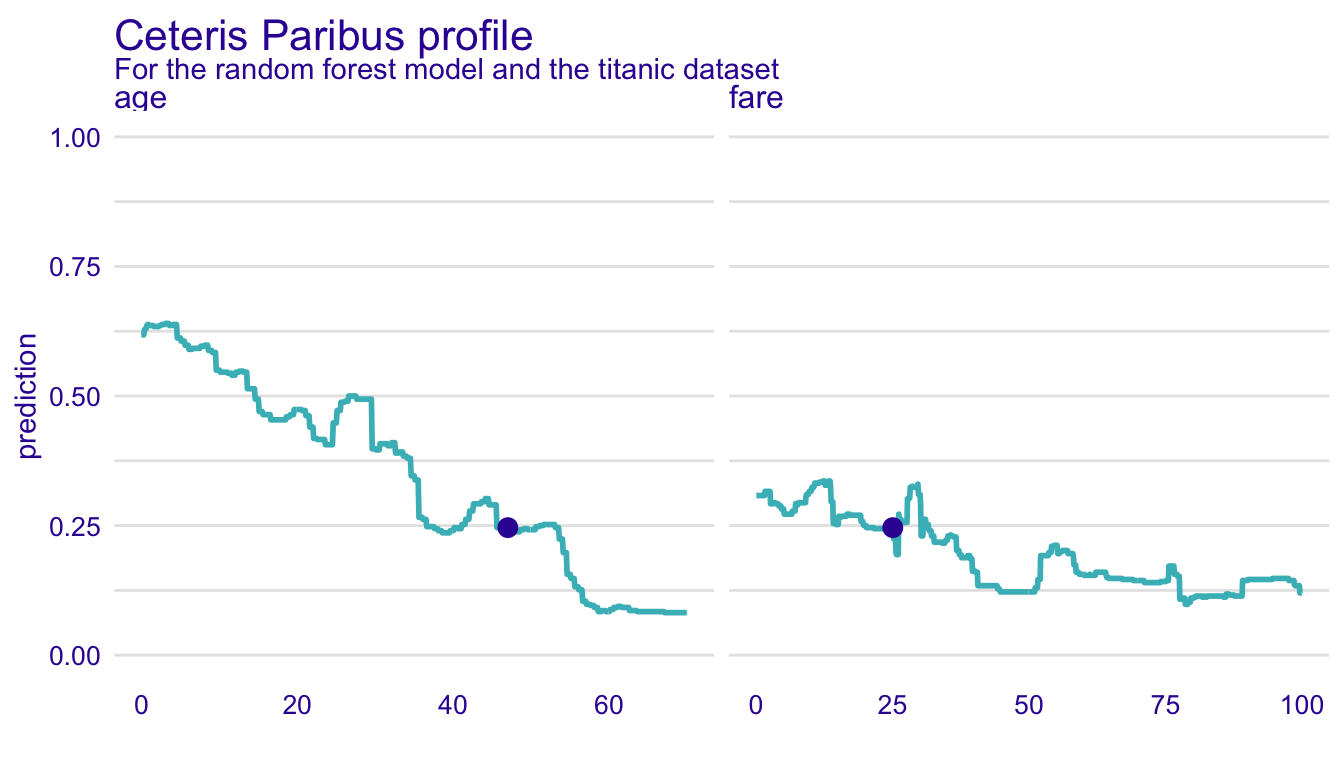
\includegraphics[width=0.7\linewidth]{PM_VEE_files/figure-latex/titanicCeterisProfile01C-1}

\}

\textbackslash{}caption\{Ceteris-paribus profiles for \texttt{class} and
\texttt{embarked} variables and the \texttt{titanic\_rf\_v6} model. Blue
dot stands for \texttt{henry}.\}\label{fig:titanicCeterisProfile01C}
\textbackslash{}end\{figure\}

To enhance the plot, additional functions can be used. The generic
\texttt{plot()} function creates a \texttt{ggplot2} object with a single
\texttt{geom\_line} layer. Function \texttt{show\_observations} adds
\texttt{geom\_point} layer, \texttt{show\_rugs} adds
\texttt{geom\_rugs}, while \texttt{show\_profiles} adds another
\texttt{geom\_line}. All these functions take, as the first argument, an
object created with the \texttt{ceteris\_paribus} function. They can be
combined freely to superpose profiles for different models or
observations.

In the example below, we present the code to create XO profiles for two
passengers, \texttt{henry} and \texttt{johny\_d}. Their profiles are
included in a plot presented in Figure
\ref{fig:titanicCeterisProfile01D}. We use the
\texttt{scale\_color\_manual} function to add names of passengers to the
plot, and to control colors and positions.

\begin{Shaded}
\begin{Highlighting}[]
\NormalTok{johny_d <-}\StringTok{ }\NormalTok{archivist}\OperatorTok{::}\KeywordTok{aread}\NormalTok{(}\StringTok{"pbiecek/models/e3596"}\NormalTok{)}
\NormalTok{cp_titanic_rf2 <-}\StringTok{ }\KeywordTok{ceteris_paribus}\NormalTok{(explain_rf_v6, }\KeywordTok{rbind}\NormalTok{(henry, johny_d))}
\end{Highlighting}
\end{Shaded}

\begin{Shaded}
\begin{Highlighting}[]
\KeywordTok{plot}\NormalTok{(cp_titanic_rf2, }\DataTypeTok{color =} \StringTok{"_ids_"}\NormalTok{) }\OperatorTok{+}\StringTok{ }
\StringTok{  }\KeywordTok{show_observations}\NormalTok{(cp_titanic_rf2, }\DataTypeTok{size =} \DecValTok{5}\NormalTok{, }\DataTypeTok{variables =} \KeywordTok{c}\NormalTok{(}\StringTok{"age"}\NormalTok{, }\StringTok{"fare"}\NormalTok{)) }\OperatorTok{+}\StringTok{ }
\StringTok{  }\KeywordTok{show_rugs}\NormalTok{(cp_titanic_rf2, }\DataTypeTok{sides =} \StringTok{"bl"}\NormalTok{, }\DataTypeTok{variables =} \KeywordTok{c}\NormalTok{(}\StringTok{"age"}\NormalTok{, }\StringTok{"fare"}\NormalTok{)) }\OperatorTok{+}\StringTok{ }
\StringTok{  }\KeywordTok{scale_color_manual}\NormalTok{(}\DataTypeTok{name =} \StringTok{"Passenger:"}\NormalTok{, }\DataTypeTok{breaks =} \DecValTok{1}\OperatorTok{:}\DecValTok{2}\NormalTok{, }\DataTypeTok{values =} \KeywordTok{c}\NormalTok{(}\StringTok{"#4378bf"}\NormalTok{, }\StringTok{"#8bdcbe"}\NormalTok{), }\DataTypeTok{labels =} \KeywordTok{c}\NormalTok{(}\StringTok{"henry"}\NormalTok{ , }\StringTok{"johny_d"}\NormalTok{)) }\OperatorTok{+}\StringTok{ }
\StringTok{  }\KeywordTok{ggtitle}\NormalTok{(}\StringTok{"Ceteris Paribus Profiles"}\NormalTok{, }\StringTok{"For the random forest model and the Titanic dataset"}\NormalTok{)}
\end{Highlighting}
\end{Shaded}

\textbackslash{}begin\{figure\}

\{\centering 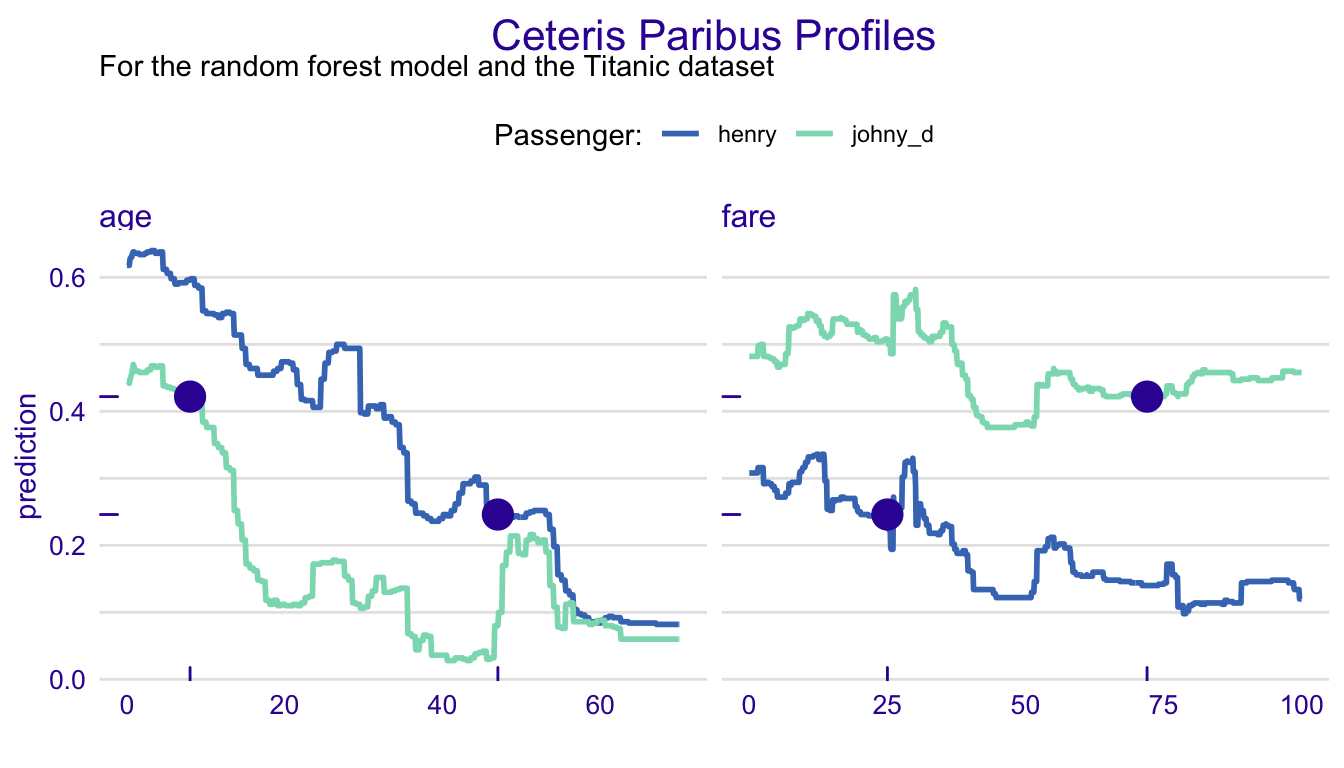
\includegraphics[width=0.7\linewidth]{PM_VEE_files/figure-latex/titanicCeterisProfile01D-1}

\}

\textbackslash{}caption\{Ceteris-paribus profiles for the
\texttt{titanic\_rf\_v6} model. Profiles for different passangers are
color-coded.\}\label{fig:titanicCeterisProfile01D}
\textbackslash{}end\{figure\}

\hypertarget{champion-challenger-analysis}{%
\subsubsection{Champion-challenger
analysis}\label{champion-challenger-analysis}}

One of the most interesting uses of the explainers is comparison of CP
profiles for two or more of models.

To illustrate this possibility, first, we have go to construct profiles
for the models. In our illustration, for the sake of clarity, we limit
ourselves just to two models: the logistic regression and random forest
models for the Titanic data. Moreover, we only consider the \texttt{age}
and \texttt{fare} variables. We use \texttt{henry} as the instance, for
which predictions are of interest.

\begin{Shaded}
\begin{Highlighting}[]
\NormalTok{cp_titanic_rf <-}\StringTok{ }\KeywordTok{ceteris_paribus}\NormalTok{(explain_rf_v6, henry)}
\NormalTok{cp_titanic_lmr <-}\StringTok{ }\KeywordTok{ceteris_paribus}\NormalTok{(explain_lmr_v6, henry)}
\end{Highlighting}
\end{Shaded}

Subsequently, we construct the plot. The result is shown in Figure
\ref{fig:titanicCeterisProfile01E}. Predictions for \texttt{henry} are
slightly different, logistic regression returns in this case higher
predictions then random forest. For \texttt{age} variable profiles of
both models are similar, in both models we see decreasing dependency.
While for \texttt{fare} the logistic regression model is slightly
positive while random forest is negative. The larger the \texttt{fare}
the larger is difference between these models. Such analysis helps us to
which degree different models agree on what if scenarios.

Note that every \texttt{plot} and \texttt{show\_*} function can take a
collection of explainers as arguments. Profiles for different models are
included in a single plot. In the presented R snippet, models are
color-coded with the help of the argument
\texttt{color\ =\ "\_label\_"}, where \texttt{\_label\_} refers to the
name of the column in the CP explainer that contains the model label.

\begin{Shaded}
\begin{Highlighting}[]
\KeywordTok{plot}\NormalTok{(cp_titanic_rf, cp_titanic_lmr, }\DataTypeTok{color =} \StringTok{"_label_"}\NormalTok{) }\OperatorTok{+}
\StringTok{  }\KeywordTok{show_observations}\NormalTok{(cp_titanic_rf, cp_titanic_lmr, }\DataTypeTok{color =} \StringTok{"black"}\NormalTok{, }\DataTypeTok{variables =} \KeywordTok{c}\NormalTok{(}\StringTok{"age"}\NormalTok{, }\StringTok{"fare"}\NormalTok{), }\DataTypeTok{size =} \DecValTok{5}\NormalTok{) }\OperatorTok{+}
\StringTok{  }\KeywordTok{scale_color_discrete}\NormalTok{(}\DataTypeTok{name =} \StringTok{"Selected models:"}\NormalTok{) }\OperatorTok{+}\StringTok{ }\KeywordTok{ylim}\NormalTok{(}\DecValTok{0}\NormalTok{,}\DecValTok{1}\NormalTok{) }\OperatorTok{+}\StringTok{ }
\StringTok{  }\KeywordTok{ggtitle}\NormalTok{(}\StringTok{"Ceteris Paribus Profiles for Henry"}\NormalTok{)}
\end{Highlighting}
\end{Shaded}

\textbackslash{}begin\{figure\}

\{\centering 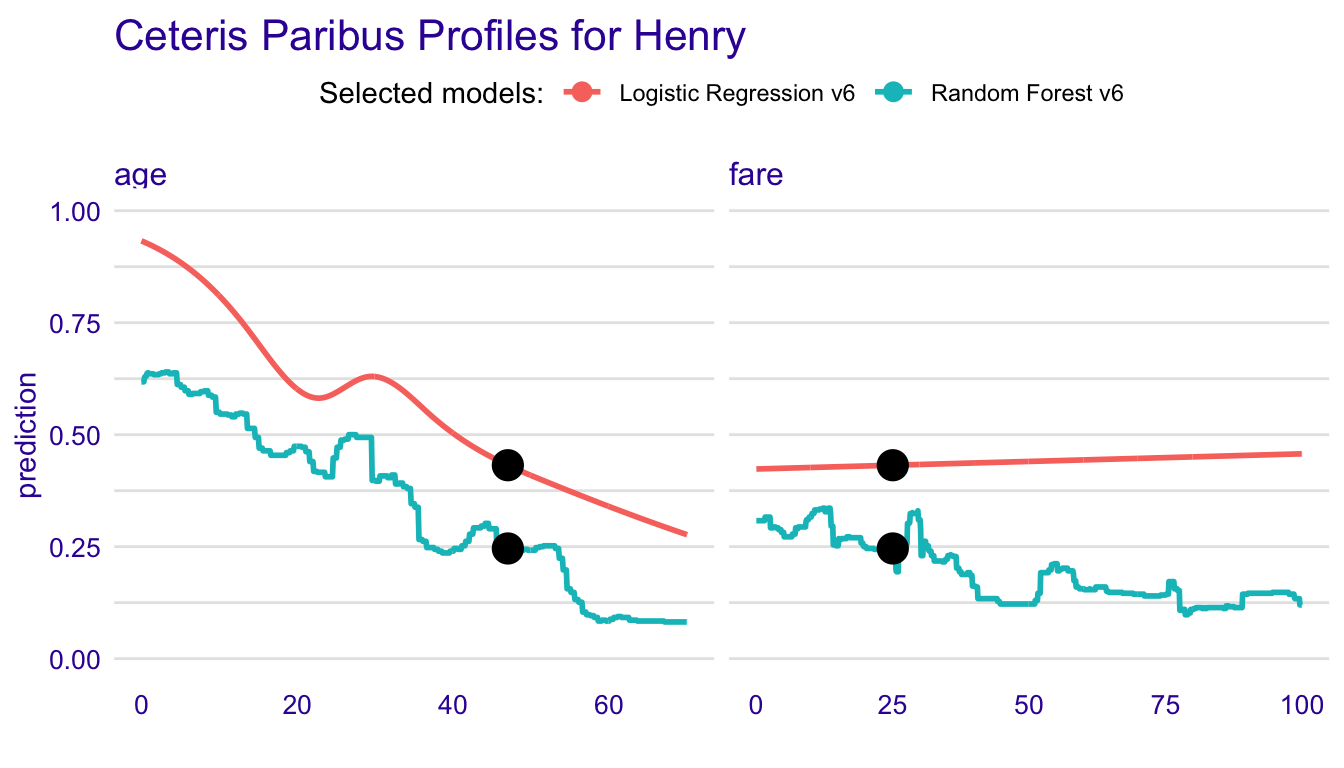
\includegraphics[width=0.7\linewidth]{PM_VEE_files/figure-latex/titanicCeterisProfile01E-1}

\}

\textbackslash{}caption\{Champion-challenger comparison of the
\texttt{titanic\_lmr\_v6} and \texttt{titanic\_rf\_v6} models. Profiles
for different models are color-coded.\}\label{fig:titanicCeterisProfile01E}
\textbackslash{}end\{figure\}

\hypertarget{ceterisParibusOscillations}{%
\section{Ceteris-paribus Oscillations and Local
Variable-importance}\label{ceterisParibusOscillations}}

\hypertarget{CPOscIntro}{%
\subsection{Introduction}\label{CPOscIntro}}

Visual examination of Ceteris-paribus (CP) profiles is insightful, but
for a model with a large number of explanatory variables we may end up
with a large number of plots which may be overwhelming. To prioritize
between the profiles we need a measure that would summarize the impact
of a selected variable on model's predictions. In this chapter we
describe a solution closely linked with CP profiles. An alternative is
discussed in the Chapters \ref{breakDown} and \ref{shapley}.

\hypertarget{CPOscIntuition}{%
\subsection{Intuition}\label{CPOscIntuition}}

To assign importance to CP profiles, we can use the concept of profile
oscillations. In particular, the larger influence of an explanatory
variable on prediction at a particular instance, the larger the
fluctuations along the corresponding CP profile. For a variable that
exercises little or no influence on model prediction, the profile will
be flat or will barely change. In other words, the values of the CP
profile should be close to the value of the model prediction for the
particular instance. Consequently, the sum of differences between the
profile and the value of the prediction, take across all possible values
of the explanatory variable, should be close to zero. The sum can be
graphically depicted by the area between the profile and the horizontal
line representing the instance prediction. On the other hand, for an
explanatory variable with a large influence on the prediction, the area
should be large. Figure \ref{fig:CPVIPprofiles} illustrates the concept.
Panle A of the figure corresponds to the CP profiles presented in Figure
\ref{fig:profileV4Rf}. The larger the highlighted area in Figure
\ref{fig:CPVIPprofiles}, the more important is the variable for the
particular prediction.

\textbackslash{}begin\{figure\}

\{\centering 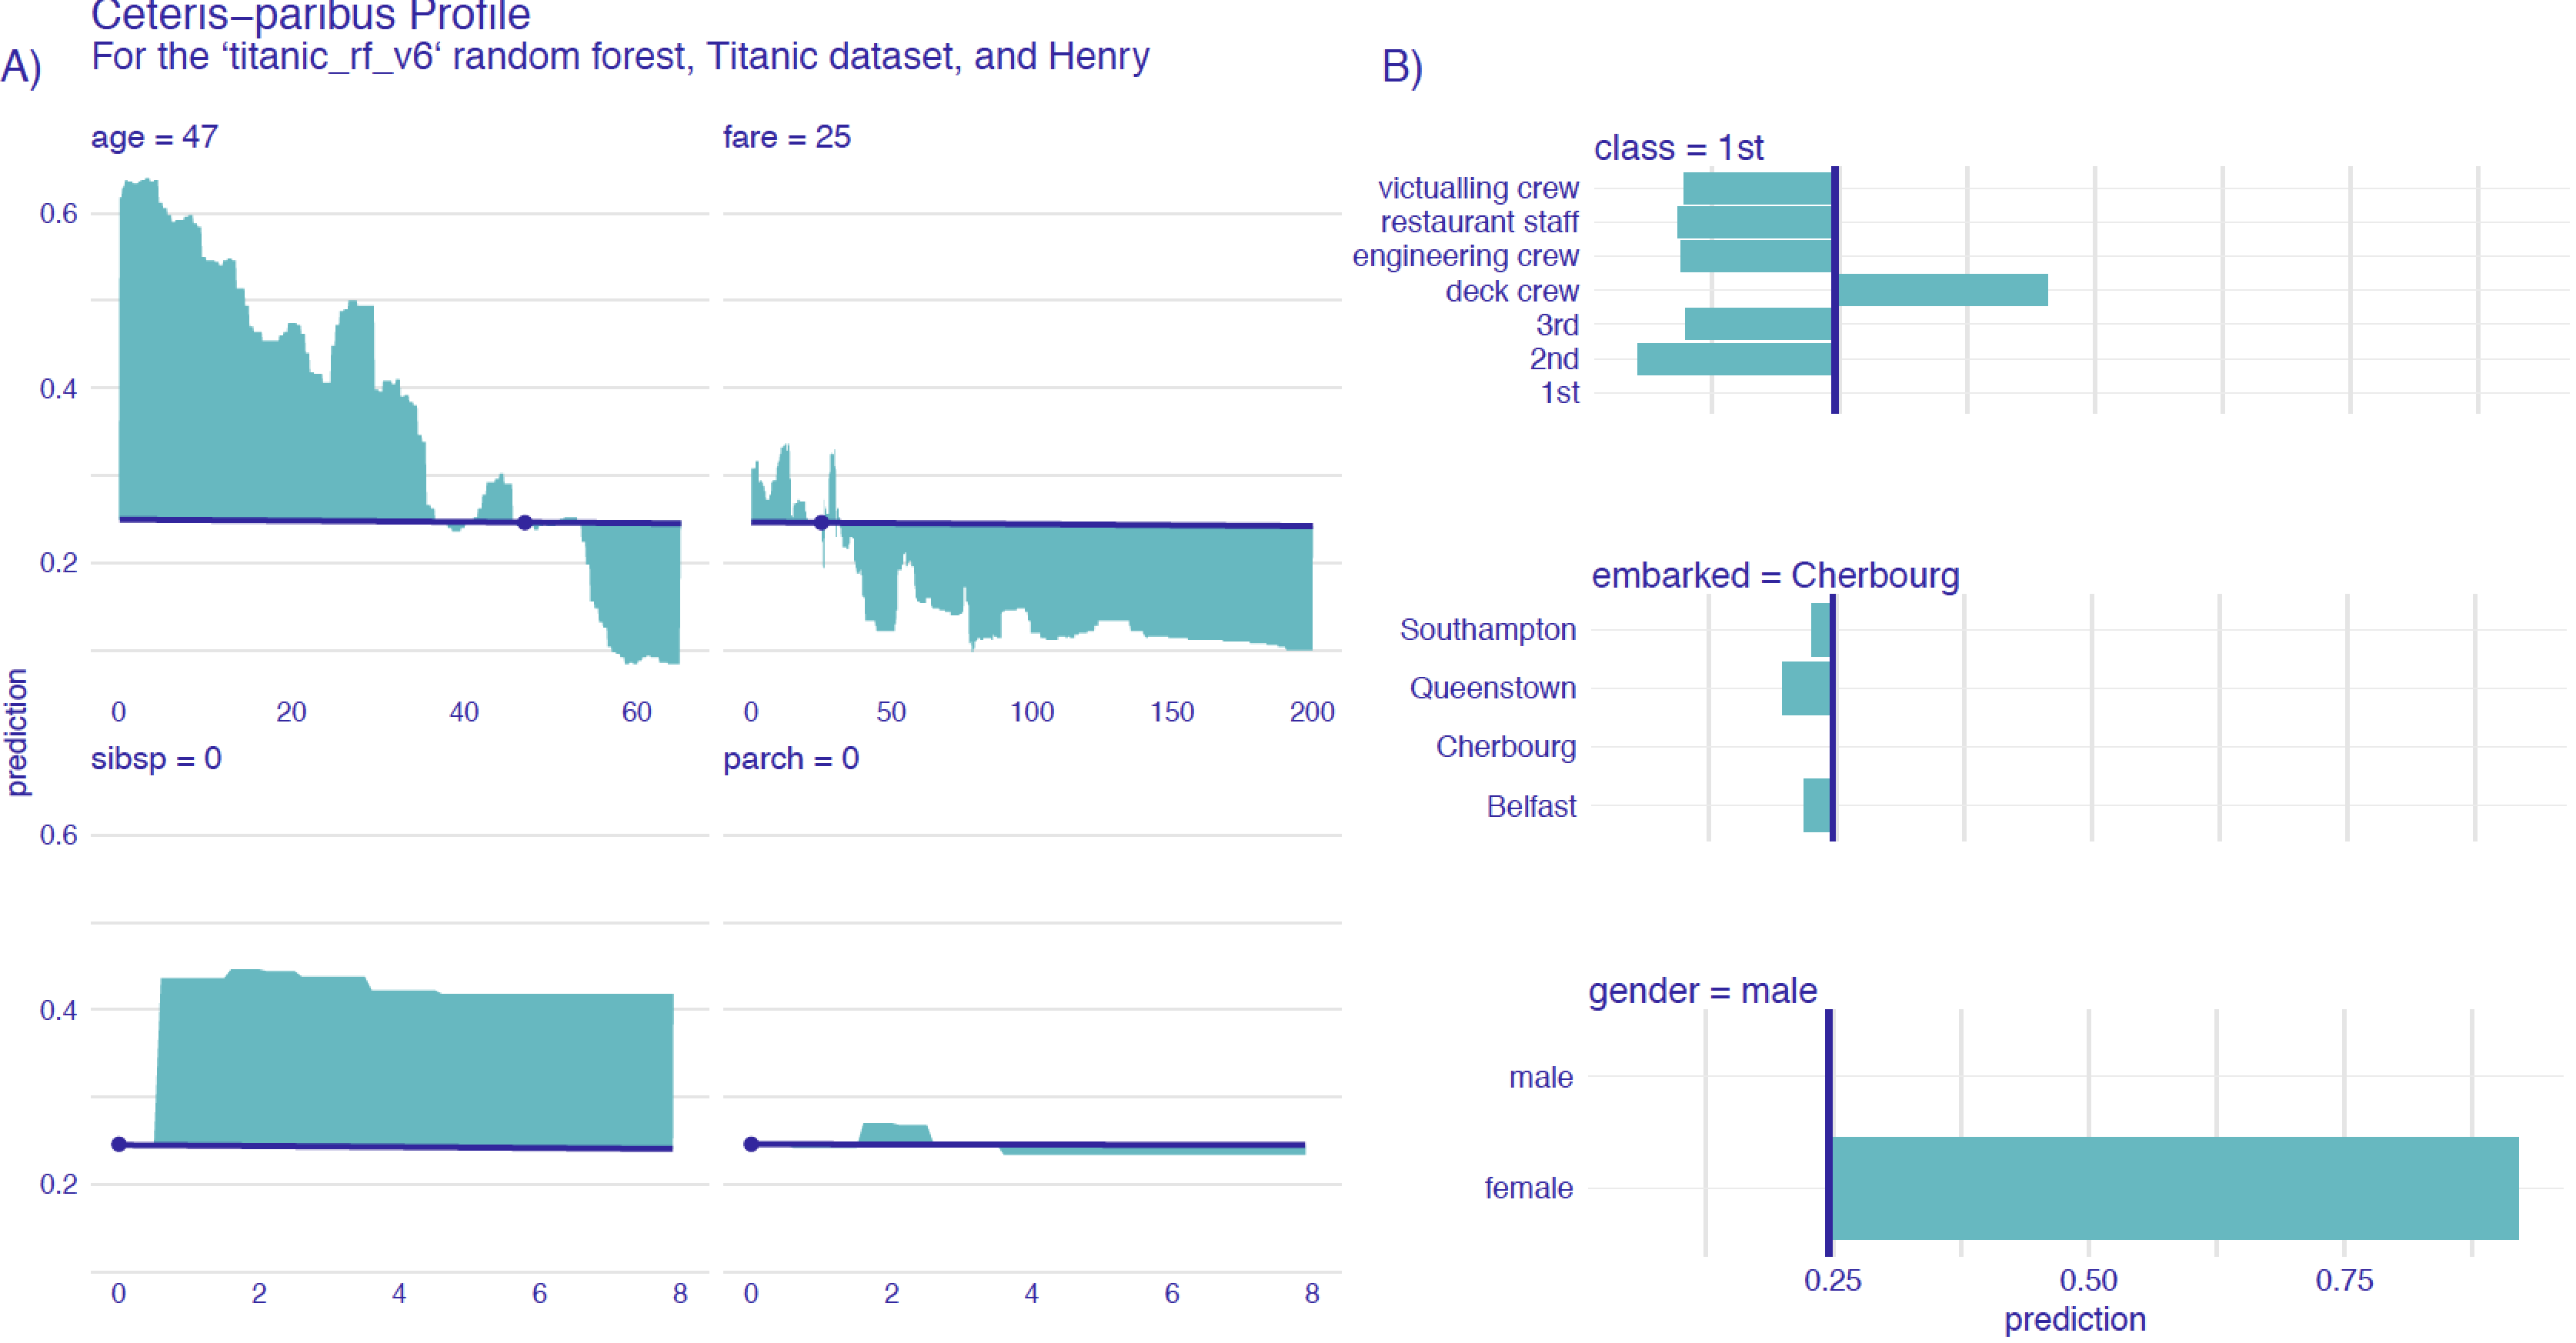
\includegraphics[width=0.99\linewidth]{figure/profile_v4_rf2}

\}

\textbackslash{}caption\{(fig:CPVIPprofiles) The value of the colored
area summarizes the Ceteris-paribus-profile oscillations and provides
the mean of the absolute deviations between the CP profile and the
instance prediction. Panel A shows plots for continuous explanatory
variables, while panel B shows plots for categorical variables in the
\texttt{titanic\_rf\_v6} model.\}\label{fig:CPVIPprofiles}
\textbackslash{}end\{figure\}

\hypertarget{CPOscMethod}{%
\subsection{Method}\label{CPOscMethod}}

Let us formalize this concept now. Denote by \(g^j(z)\) the probability
density function of the distribution of the \(j\)-th explanatory
variable. The summary measure of the variable's importance for model
prediction at point \(x_*\), \(vip_{CP}^{j}(x_*)\), computed based on
the variable's CP profile, is defined as follows:

\begin{equation}
vip_{CP}^j(x_*) = \int_{\mathcal R} |h^{j}_{x_*}(z) - f(x_*)| g^j(z)dz=E_{X^j}\left[|h^{j}_{x_*}(X^j) - f(x_*)|\right].
\label{eq:VIPCPdef}
\end{equation}

Thus, \(vip_{CP}^j(x_*)\) is the expected absolute deviation of the CP
profile from the model prediction for \(x_*\) over the distribution
\(g^j(z)\) for the \(j\)-th explanatory variable.

The true distribution of \(j\)-th explanatory variable is, in most
cases, unknown. Thus, there are several options how to calculate
\eqref{eq:VIPCPdef}.

One is to calculate just the area under the CP curve, i.e., to assume
that \(g^j(z)\) is a uniform distribution for the range of variable
\(x^j\). It folows then that a straightforward estimator of
\(vip_{CP}^{j,uni}(x_*)\) is

\begin{equation}
\widehat{vip}_{CP}^{j,uni}(x_*) = \frac 1k \sum_{l=1}^k |h^{j}_{x_*}(z_l) - f(x_*)|,
\label{eq:VIPCPuni}
\end{equation}

where \(z_l\) (\(l=1, \ldots, k\)) are the selected values of the
\(j\)-th explanatory variable. For instance, one can select use all
unique values of \(x^{j}\) in the considered dataset. Alternatively, for
a continuous variable, one can use an equi-distant grid of values.

Another approach is to use the empirical distribution for \(x^{j}\).
This leads to the estimator of \(vip_{CP}^{j,emp}(x_*)\) defined as

\begin{equation}
\widehat{vip}_{CP}^{j,emp}(x_*) = \frac 1n \sum_{i=1}^n |h^{j}_{x_*}(x^{j}_i) - f(x_*)|,
\label{eq:VIPCPemp}
\end{equation}

where index \(i\) goes through all observations in a dataset.

The use of of \(\widehat{vip}_{CP}^{j,emp}(x_*)\) is preferred when
there are enough data to accurately estimate the empirical distribution
and when the distribution is not uniform. On the other hand,
\(\widehat{vip}_{CP}^{j,uni}(x_*)\) is in most cases quicker to compute
and, therefore, it is preferred if we look for fast approximations.

It is worth noting that the importance of an explanatory variable for
instance prediction may be very different for different points \(x_*\).
For example, consider model \[
f(x_1, x_2) = x_1 * x_2,
\] where \(x_1\) and \(x_2\) take values in \([0,1]\). Consider
prediction for an observation described by vector \(x_* = (0,1)\). In
that case, the importance of \(X_1\) is larger than \(X_2\). This is
because the CP profile for the first variable, given by the values of
function \(f(z,1)=z\), will have oscillations. On the other hand, the
profile for the second variable will show no oscillations, because the
profile is given by function \(f(0,z)=0\). Obviously, the situation is
reversed for \(x_*=(1,0)\).

\hypertarget{CPOscExample}{%
\subsection{Example: Titanic}\label{CPOscExample}}

Figure \ref{fig:CPVIP1} provides a barplot of variable importance
measures for different continuous explanatory variables for the random
forest model \texttt{titanic\_rf\_v6} for \texttt{henry}.

The longer the bar, the larger the CP-profile oscillations for a
particular explanatory variable. Thus, Figure \ref{fig:CPVIP1} indicates
that the most important variable for prediction for the selected
observation are \texttt{gender} and \texttt{sibsp}, followed by
\texttt{age}.

From the Ceteris Paribus one can read that if Henry were older, this
would significantly lower the chance of survival. One the other hand,
were Henry not travelling alone, this would increase the chance.

From the oscillation's plot one can only read which features are
important but one cannot read how they influence the prediction. This is
why profile oscillations shall be accompanied by Ceteris Paribus
profiles.

\textbackslash{}begin\{figure\}

\{\centering 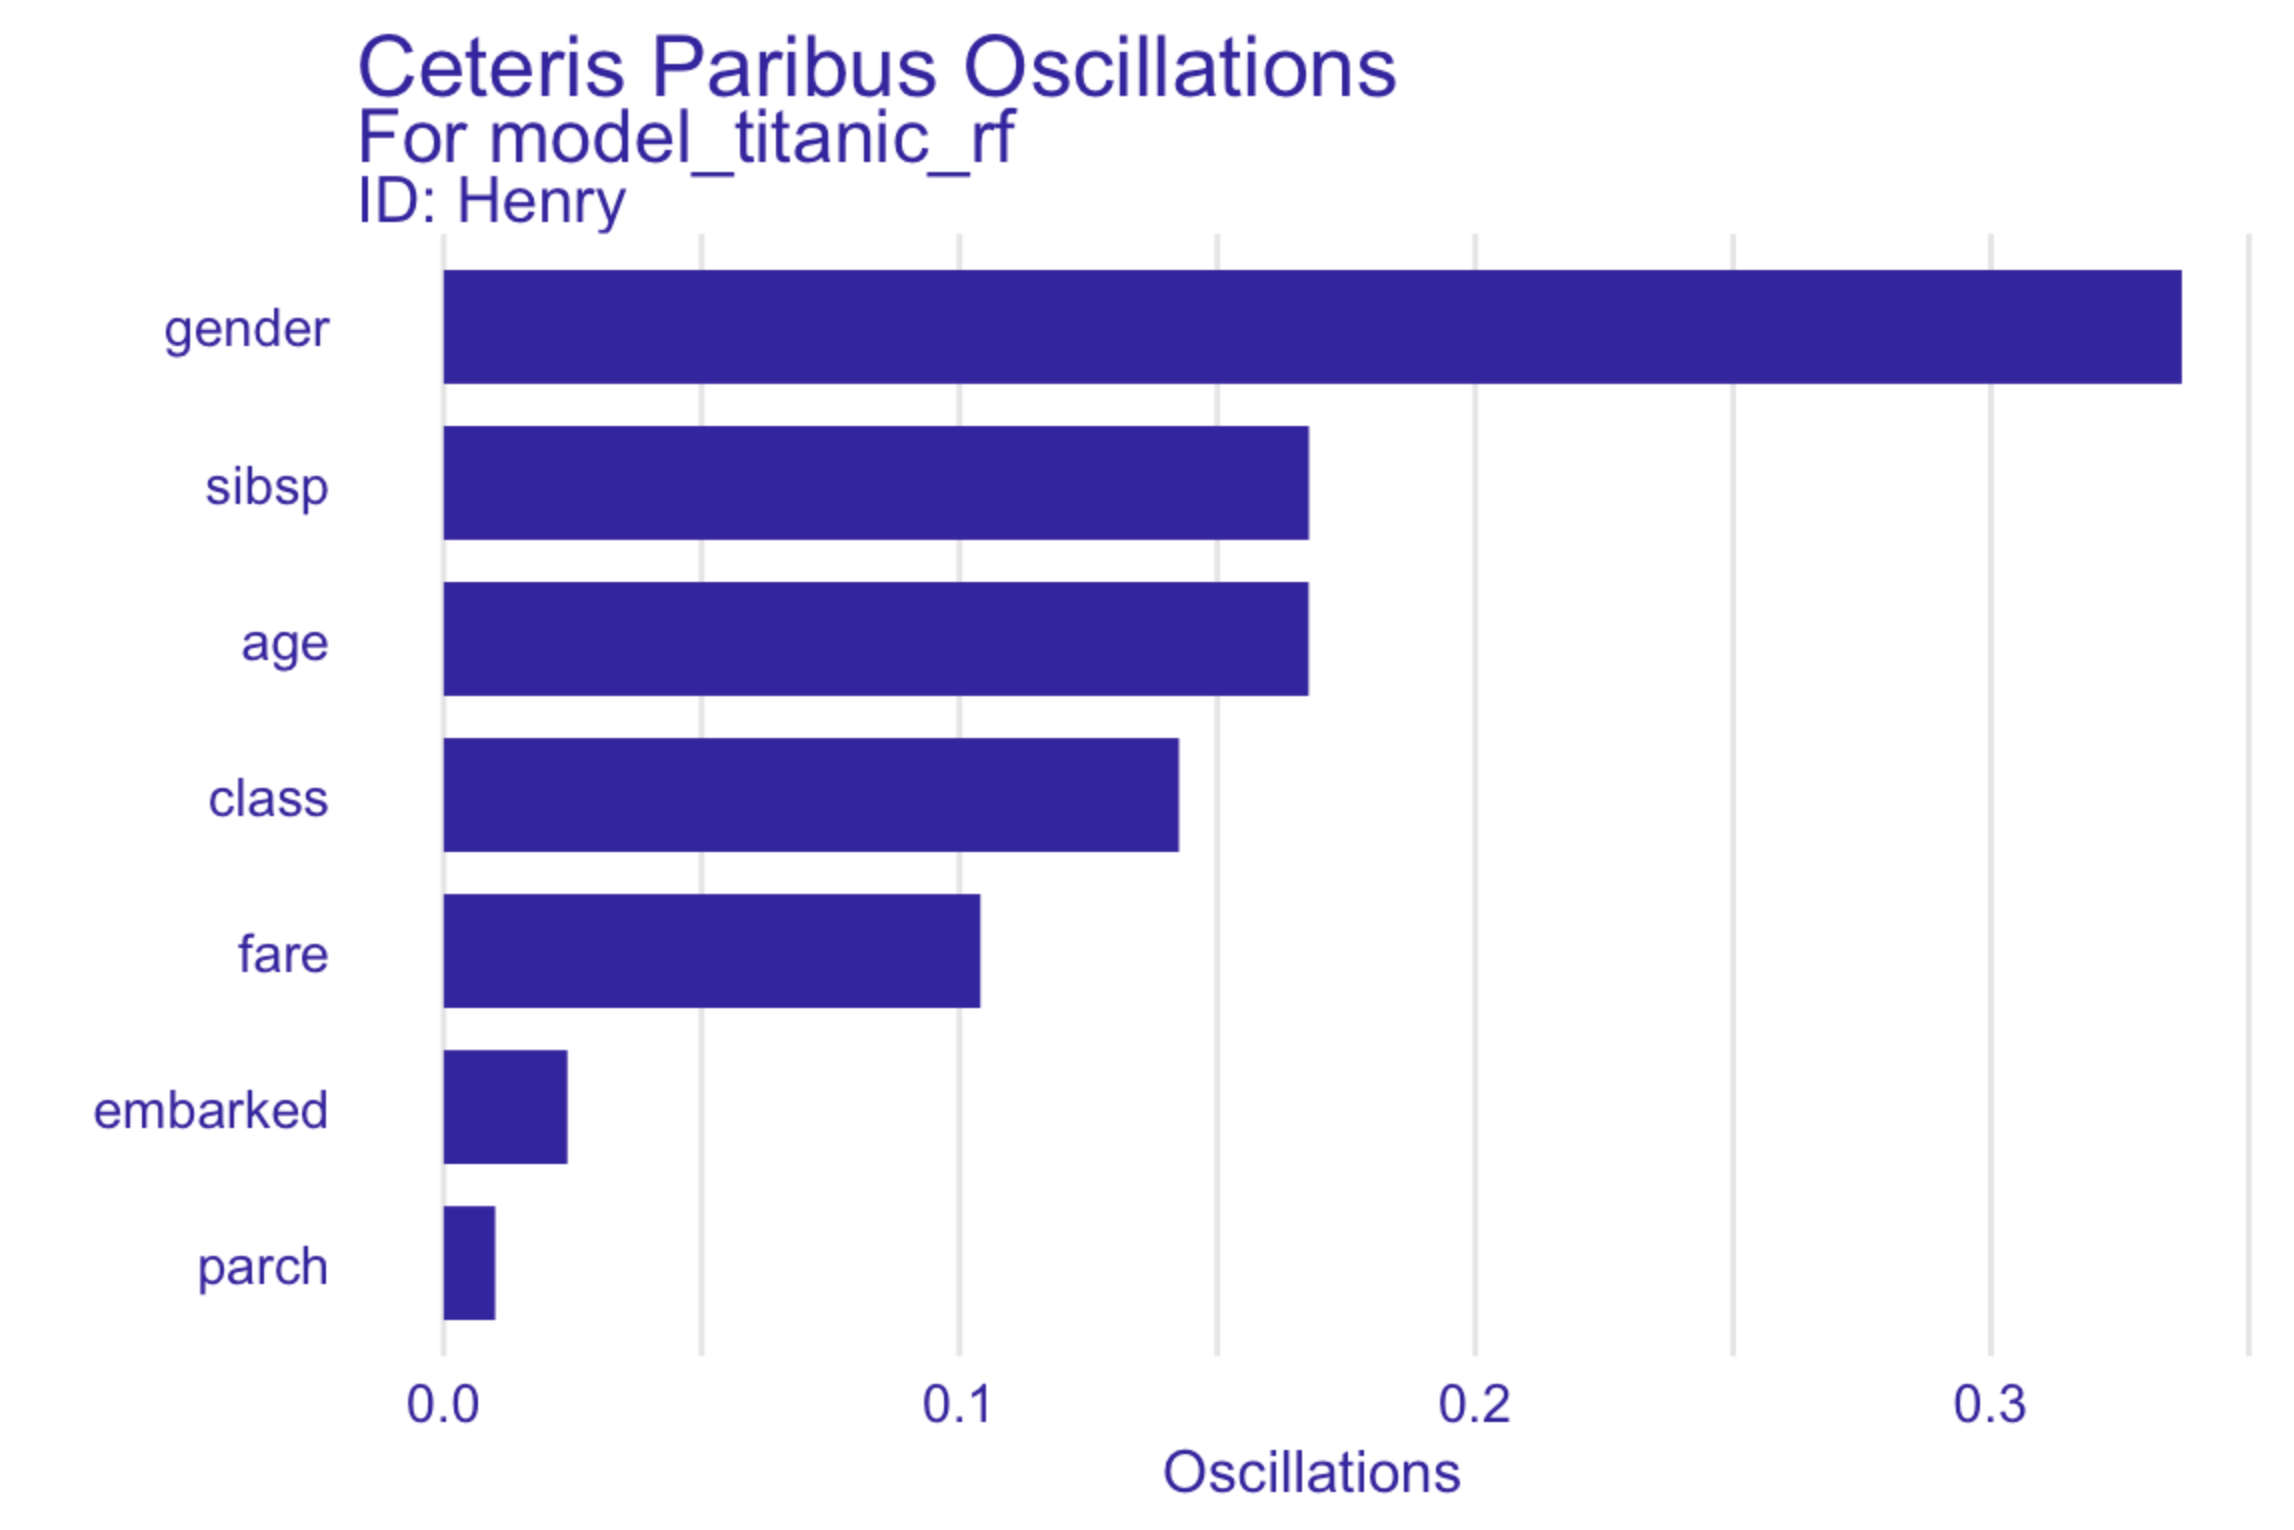
\includegraphics[width=0.75\linewidth]{figure/oscillations_all_rf_plot}

\}

\textbackslash{}caption\{(fig:CPVIP1) Variable-importance measures
calculated for Ceteris-paribus oscillations for \texttt{henry} based on
the \texttt{titanic\_rf\_v6} model\}\label{fig:CPVIP1}
\textbackslash{}end\{figure\}

\hypertarget{CPOscProsCons}{%
\subsection{Pros and cons}\label{CPOscProsCons}}

Oscillations of CP profiles are easy to interpret and understand. By
using the average of oscillations, it is possible to select the most
important variables for an instance prediction. The methodology can
easily be extended to two or more variables.

There are several issues related to the use of the CP oscillations. For
example, the oscillations may not be of help in situations when the use
of CP profiles may itself be problematic (e.g., in the case of
correlated explanatory variables or interactions - see Section
\ref{CPProsCons}). An important issue is that the local variable
importance do not sum up to the instance prediction for which they are
calculated. In Chapters \ref{breakDown} and \ref{shapley}, we will
introduce measures that address this problem.

\hypertarget{CPOscR}{%
\subsection{Code snippets for R}\label{CPOscR}}

In this section, we present key features of R package
\texttt{ingredients} which is a part of the \texttt{DrWhy.AI} universe
and covers all methods presented in this chapter. More details and
examples can be found at
\url{https://modeloriented.github.io/ingredients/}.

For illustration purposes we use the random forest model
\texttt{titanic\_rf\_v6} (see Section \ref{odel-HR-rf}). Recall that it
is developed to predict the probability of survival from sinking of
Titanic. Instance-level explanations are calculated for a single
observation: \texttt{henry} - a 47-year-old passenger that travelled in
the 1st class.

\texttt{DALEX} explainers for both models and the Henry data are
retrieved via \texttt{archivist} hooks as listed in Section
\ref{ListOfModelsTitanic}.

\begin{Shaded}
\begin{Highlighting}[]
\KeywordTok{library}\NormalTok{(}\StringTok{"randomForest"}\NormalTok{)}
\NormalTok{explain_rf_v6 <-}\StringTok{ }\NormalTok{archivist}\OperatorTok{::}\KeywordTok{aread}\NormalTok{(}\StringTok{"pbiecek/models/9b971"}\NormalTok{)}

\KeywordTok{library}\NormalTok{(}\StringTok{"DALEX"}\NormalTok{)}
\NormalTok{henry <-}\StringTok{ }\NormalTok{archivist}\OperatorTok{::}\KeywordTok{aread}\NormalTok{(}\StringTok{"pbiecek/models/a6538"}\NormalTok{)}
\NormalTok{henry}
\end{Highlighting}
\end{Shaded}

\hypertarget{basic-use-of-the-calculate_oscillations-function}{%
\subsubsection{\texorpdfstring{Basic use of the
\texttt{calculate\_oscillations}
function}{Basic use of the calculate\_oscillations function}}\label{basic-use-of-the-calculate_oscillations-function}}

To calculate CP oscillations, we have got to calculate CP profiles for
the selected observation. We use \texttt{henry} as the instance
prediction of interest.

CP profiles are calculated by applying the \texttt{ceteris\_paribus()}
function to the wrapper object.

\begin{Shaded}
\begin{Highlighting}[]
\KeywordTok{library}\NormalTok{(}\StringTok{"ingredients"}\NormalTok{)}
\KeywordTok{library}\NormalTok{(}\StringTok{"ggplot2"}\NormalTok{)}

\NormalTok{cp_titanic_rf <-}\StringTok{ }\KeywordTok{ceteris_paribus}\NormalTok{(explain_rf_v6, henry)}
\end{Highlighting}
\end{Shaded}

The resulting object can subsequently be processed with the
\texttt{calculate\_oscillations()} function to calculate the
oscillations and the estimated value of the variable-importance measure
\eqref{eq:VIPCPdef}.

\begin{Shaded}
\begin{Highlighting}[]
\NormalTok{oscillations_titanic_rf <-}\StringTok{ }\KeywordTok{calculate_oscillations}\NormalTok{(cp_titanic_rf)}
\NormalTok{oscillations_titanic_rf}
\end{Highlighting}
\end{Shaded}

\begin{verbatim}
##    _vname_ _ids_ oscillations
## 2   gender     1   0.33700000
## 4    sibsp     1   0.15500000
## 3      age     1   0.14700000
## 1    class     1   0.14257143
## 6     fare     1   0.05407273
## 7 embarked     1   0.02400000
## 5    parch     1   0.00800000
\end{verbatim}

Note that, by default, \texttt{calculate\_oscillations()} estimates
\(vip_{CP}^j(x_*)\) by \(\widehat{vip}_{CP}^{j,uni}(x_*)\), given in
\eqref{eq:VIPCPuni}, using all unique values of the explanatory variable
as the grid points.

The \texttt{calculate\_oscillations()} function returns an object of
class \texttt{ceteris\_paribus\_oscillations}, which has a form of a
data frame, but has also an overloaded \texttt{plot()} function. We can
use the latter function to plot the local variable-importance measures
for the instance of interest.

\begin{Shaded}
\begin{Highlighting}[]
\NormalTok{oscillations_titanic_rf}\OperatorTok{$}\StringTok{`}\DataTypeTok{_ids_}\StringTok{`}\NormalTok{ <-}\StringTok{ "Henry"}
\KeywordTok{plot}\NormalTok{(oscillations_titanic_rf) }\OperatorTok{+}\StringTok{ }\KeywordTok{ggtitle}\NormalTok{(}\StringTok{"Ceteris Paribus Oscillations"}\NormalTok{)}
\end{Highlighting}
\end{Shaded}

\begin{center}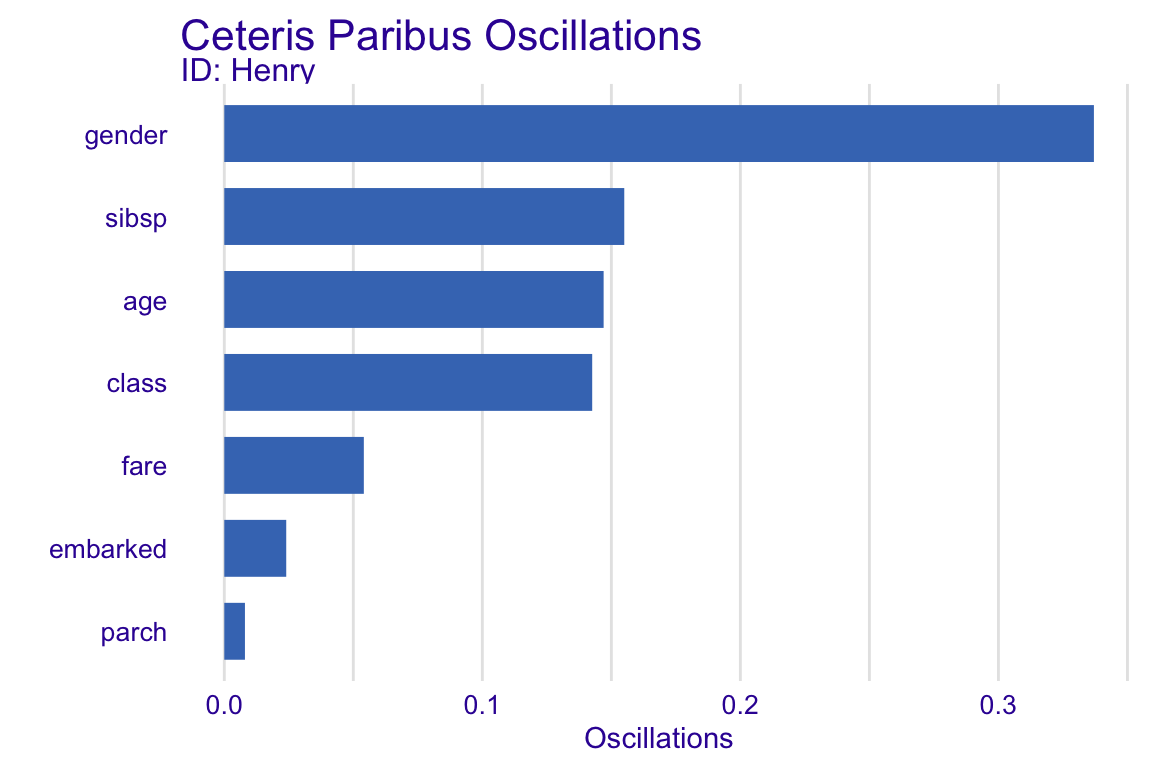
\includegraphics[width=0.7\linewidth]{PM_VEE_files/figure-latex/titanicCeterisProfile02E-1} \end{center}

\hypertarget{advanced-use-of-the-calculate_oscillations-function}{%
\subsubsection{\texorpdfstring{Advanced use of the
\texttt{calculate\_oscillations}
function}{Advanced use of the calculate\_oscillations function}}\label{advanced-use-of-the-calculate_oscillations-function}}

As mentioned in the previous section, \texttt{calculate\_oscillations()}
estimates \(vip_{CP}^j(x_*)\) by \(\widehat{vip}_{CP}^{j,uni}(x_*)\)
using all unique values of the explanatory variable as the grid points.
However, other approaches are also possible.

One is to use \(\widehat{vip}_{CP}^{j,uni}(x_*)\), but assuming an
equi-distant grid of values for a continuous explanatory variable.
Toward this aim, we have got to explicitly specify a dense uniform grid
of values for such a variable. The \texttt{variable\_splits} argument
can be used for this purpose.

\begin{Shaded}
\begin{Highlighting}[]
\NormalTok{cp_titanic_rf_uniform <-}\StringTok{ }\KeywordTok{ceteris_paribus}\NormalTok{(explain_rf_v6, henry, }
              \DataTypeTok{variable_splits =} \KeywordTok{list}\NormalTok{(}\DataTypeTok{age =} \KeywordTok{seq}\NormalTok{(}\DecValTok{0}\NormalTok{, }\DecValTok{65}\NormalTok{, }\FloatTok{0.1}\NormalTok{),}
                                     \DataTypeTok{fare =} \KeywordTok{seq}\NormalTok{(}\DecValTok{0}\NormalTok{, }\DecValTok{200}\NormalTok{, }\FloatTok{0.1}\NormalTok{),}
                                     \DataTypeTok{sibsp =} \KeywordTok{seq}\NormalTok{(}\DecValTok{0}\NormalTok{, }\DecValTok{8}\NormalTok{, }\FloatTok{0.1}\NormalTok{),}
                                     \DataTypeTok{parch =} \KeywordTok{seq}\NormalTok{(}\DecValTok{0}\NormalTok{, }\DecValTok{8}\NormalTok{, }\FloatTok{0.1}\NormalTok{),}
                                     \DataTypeTok{gender =} \KeywordTok{unique}\NormalTok{(titanic}\OperatorTok{$}\NormalTok{gender),}
                                     \DataTypeTok{embarked =} \KeywordTok{unique}\NormalTok{(titanic}\OperatorTok{$}\NormalTok{embarked),}
                                     \DataTypeTok{class =} \KeywordTok{unique}\NormalTok{(titanic}\OperatorTok{$}\NormalTok{class)))}
\end{Highlighting}
\end{Shaded}

Subsequently, we apply the \texttt{calculate\_oscillations()} function
to compute the oscillations and the variable-importance measures.

\begin{Shaded}
\begin{Highlighting}[]
\NormalTok{oscillations_uniform <-}\StringTok{ }\KeywordTok{calculate_oscillations}\NormalTok{(cp_titanic_rf_uniform)}
\NormalTok{oscillations_uniform}\OperatorTok{$}\StringTok{`}\DataTypeTok{_ids_}\StringTok{`}\NormalTok{ <-}\StringTok{ "Henry"}
\NormalTok{oscillations_uniform}
\end{Highlighting}
\end{Shaded}

\begin{verbatim}
##    _vname_ _ids_ oscillations
## 5   gender Henry    0.3370000
## 3    sibsp Henry    0.1677778
## 1      age Henry    0.1677235
## 7    class Henry    0.1425714
## 2     fare Henry    0.1040790
## 6 embarked Henry    0.0240000
## 4    parch Henry    0.0100000
\end{verbatim}

\begin{Shaded}
\begin{Highlighting}[]
\KeywordTok{plot}\NormalTok{(oscillations_uniform) }\OperatorTok{+}\StringTok{ }\KeywordTok{ggtitle}\NormalTok{(}\StringTok{"Ceteris Paribus Oscillations"}\NormalTok{, }\StringTok{"Expectation over uniform distribution"}\NormalTok{)}
\end{Highlighting}
\end{Shaded}

\begin{center}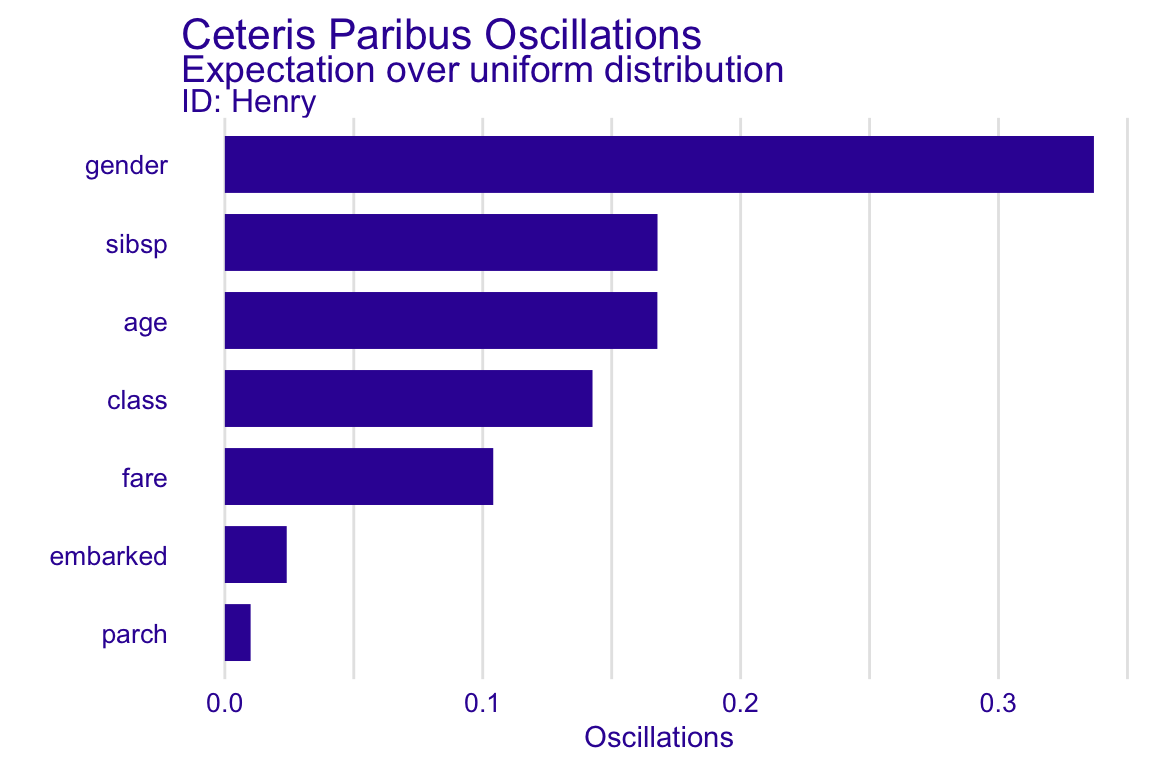
\includegraphics[width=0.7\linewidth]{PM_VEE_files/figure-latex/titanicCeterisProfile02G-1} \end{center}

Another approach is to calculate the expectation \eqref{eq:VIPCPdef} over
the empirical distribution of a variable, i..e, to use
\(\widehat{vip}_{CP}^{j,emp}(x_*)\), given in \eqref{eq:VIPCPemp}. Toward
this aim, we use the \texttt{variable\_splits} argument to explicitly
specify the validation-data sample to define the grid of values.

\begin{Shaded}
\begin{Highlighting}[]
\NormalTok{titanic <-}\StringTok{ }\KeywordTok{na.omit}\NormalTok{(titanic)}

\NormalTok{cp_titanic_rf_empirical <-}\StringTok{ }\KeywordTok{ceteris_paribus}\NormalTok{(explain_rf_v6, henry, }
              \DataTypeTok{variable_splits =} \KeywordTok{list}\NormalTok{(}\DataTypeTok{age =}\NormalTok{ titanic}\OperatorTok{$}\NormalTok{age,}
                                     \DataTypeTok{fare =}\NormalTok{ titanic}\OperatorTok{$}\NormalTok{fare,}
                                     \DataTypeTok{sibsp =}\NormalTok{ titanic}\OperatorTok{$}\NormalTok{sibsp,}
                                     \DataTypeTok{parch =}\NormalTok{ titanic}\OperatorTok{$}\NormalTok{parch,}
                                     \DataTypeTok{gender =}\NormalTok{ titanic}\OperatorTok{$}\NormalTok{gender,}
                                     \DataTypeTok{embarked =}\NormalTok{ titanic}\OperatorTok{$}\NormalTok{embarked,}
                                     \DataTypeTok{class =}\NormalTok{ titanic}\OperatorTok{$}\NormalTok{class))}
\end{Highlighting}
\end{Shaded}

\begin{Shaded}
\begin{Highlighting}[]
\NormalTok{oscillations_empirical <-}\StringTok{ }\KeywordTok{calculate_oscillations}\NormalTok{(cp_titanic_rf_empirical)}
\NormalTok{oscillations_empirical}\OperatorTok{$}\StringTok{`}\DataTypeTok{_ids_}\StringTok{`}\NormalTok{ <-}\StringTok{ "Henry"}
\NormalTok{oscillations_empirical}
\end{Highlighting}
\end{Shaded}

\begin{verbatim}
##    _vname_ _ids_ oscillations
## 1      age Henry  0.153323969
## 5   gender Henry  0.149336656
## 7    class Henry  0.133567739
## 2     fare Henry  0.056883552
## 3    sibsp Henry  0.035932034
## 6 embarked Henry  0.019818758
## 4    parch Henry  0.001623924
\end{verbatim}

\begin{Shaded}
\begin{Highlighting}[]
\KeywordTok{plot}\NormalTok{(oscillations_empirical) }\OperatorTok{+}\StringTok{ }\KeywordTok{ggtitle}\NormalTok{(}\StringTok{"Ceteris Paribus Oscillations"}\NormalTok{, }\StringTok{"Expectation over empirical distribution"}\NormalTok{)}
\end{Highlighting}
\end{Shaded}

\begin{center}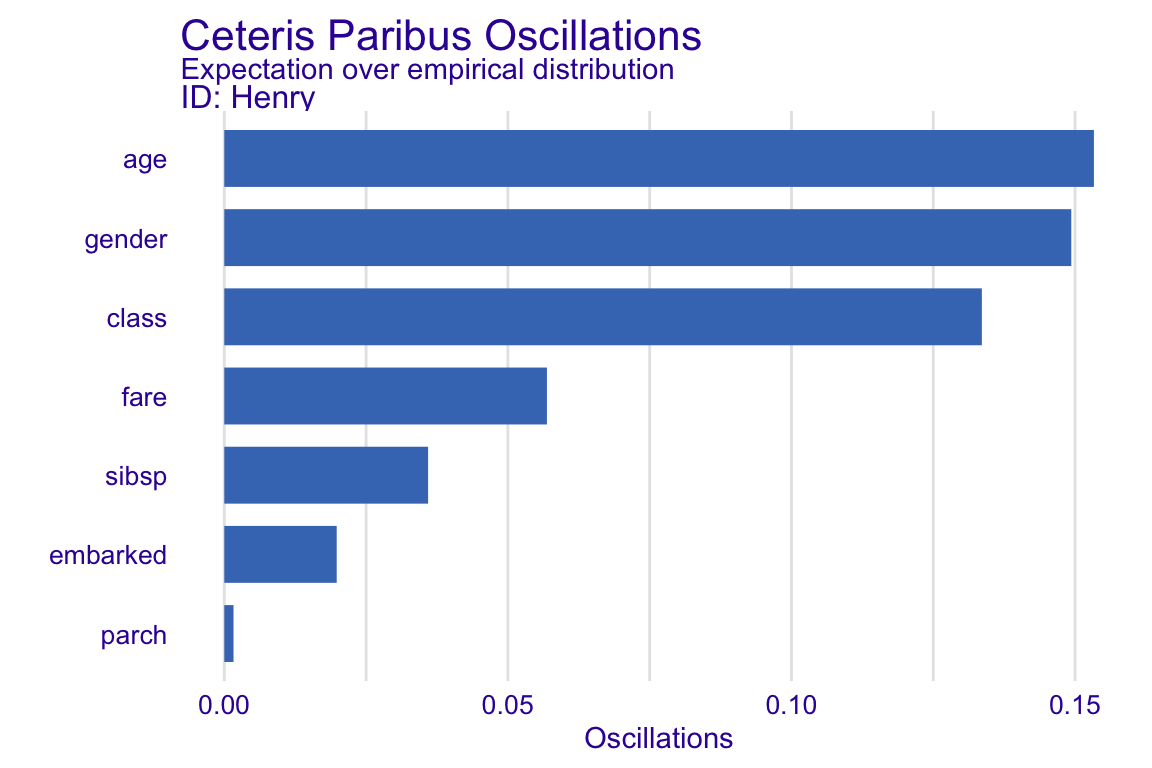
\includegraphics[width=0.7\linewidth]{PM_VEE_files/figure-latex/titanicCeterisProfile02I-1} \end{center}

\hypertarget{localDiagnostics}{%
\section{Local Diagnostics With Ceteris-paribus
Profiles}\label{localDiagnostics}}

\hypertarget{cPLocDiagIntro}{%
\subsection{Introduction}\label{cPLocDiagIntro}}

It may happen that, while the global predictive performance of the model
is good, model predictions for some observations are very bad. In this
chapter, we present two local-diagnostics techniques that can address
this issue. In particular, we focus on fidelity plots: the plot of CP
profiles for nearest neighbors and the local-fidelity plot.

The idea behind fidelity plots is to select a number of observations
(``neighbors'') from the validation dataset that are closest to the
instance (observation) of interest. Then, for the selected observations,
we plot CP profiles and check how stable they are. Additionally, if we
know true values of the dependent variable for the selected neighbors,
we may add residuals to the plot to evaluate the local fit of the model.

\hypertarget{cPLocDiagIntuition}{%
\subsection{Intuition}\label{cPLocDiagIntuition}}

One approach to local model diagnostics is to examine how the
predictions vary for observations from the training dataset. Figure
\ref{fig:profileWith10NN} presents CP profiles for the instance of
interest and its 10 nearest neighbors for the random forest model for
the Titanic dataset (Section \ref{model-titanic-rf}). The profiles are
almost parallel and very close to each other. This suggests that model
predictions are stable around the instance of interest, because small
changes in the explanatory variables (represented by the nearest
neighbors) have not got much influence on the predictions.

\textbackslash{}begin\{figure\}

\{\centering 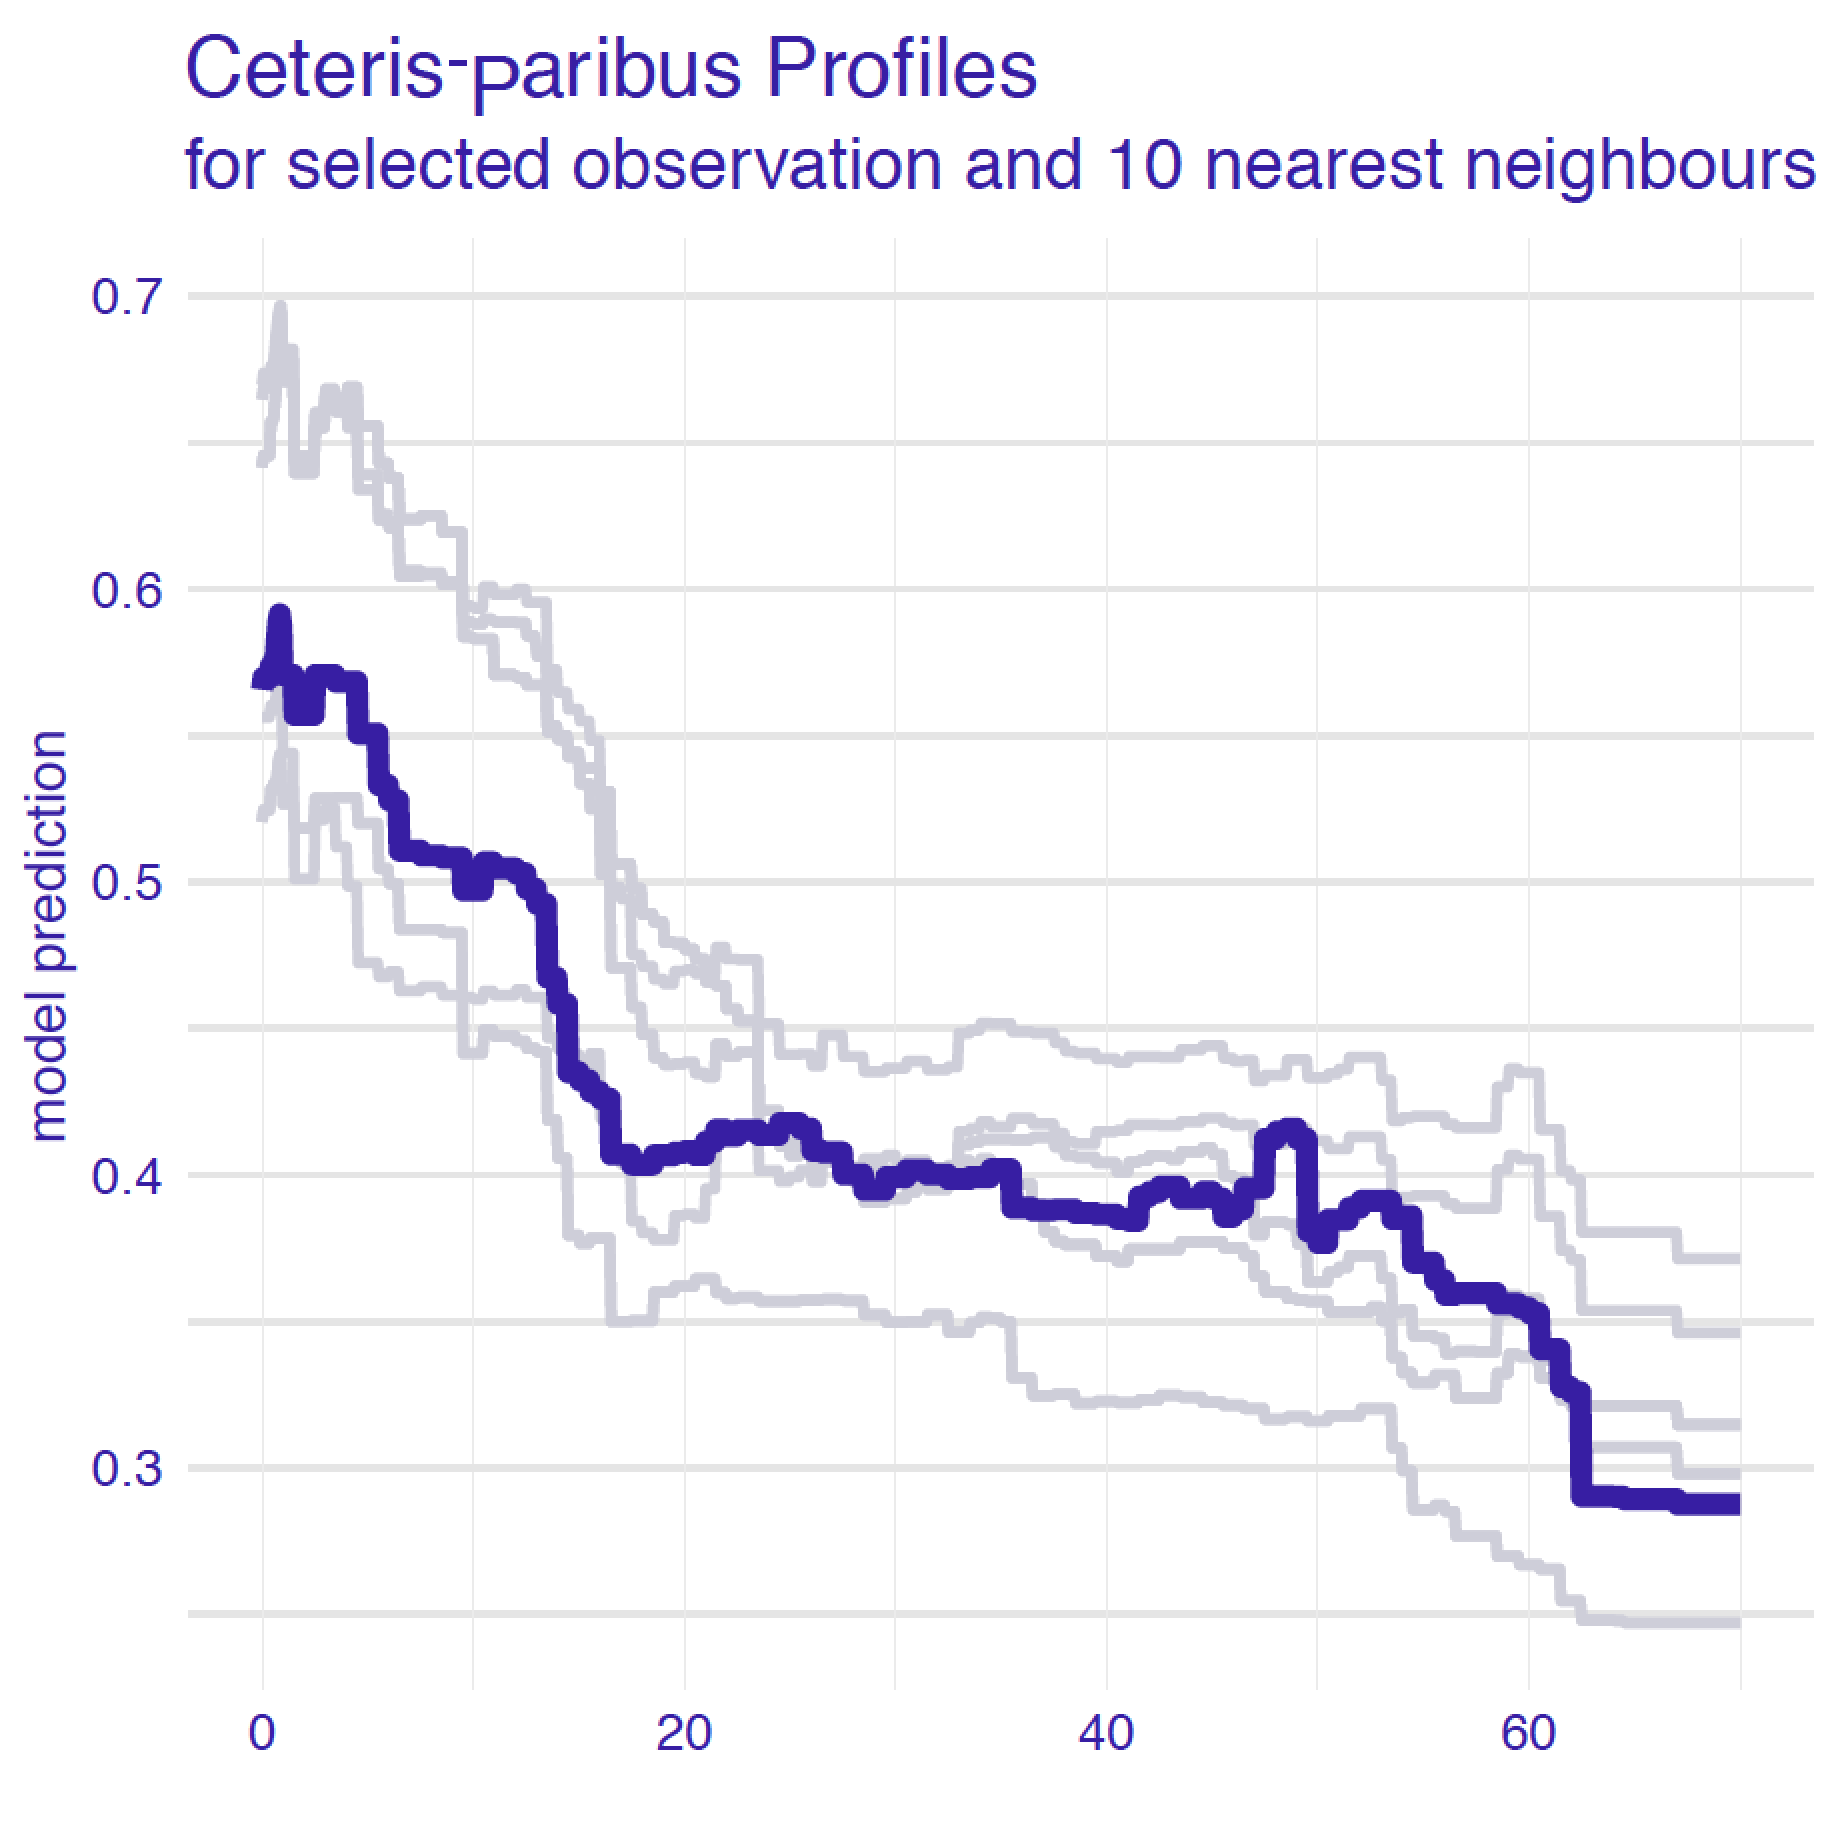
\includegraphics[width=0.5\linewidth]{figure/example_cp}

\}

\textbackslash{}caption\{(fig:profileWith10NN) Ceteris-paribus profiles
for a selected instance (dark violet line) and 10 nearest neighbors
(light grey lines) for the \texttt{titanic\_rf\_b6} model. The profiles
are almost parallel and close to each other what suggests the stability
of the model.\}\label{fig:profileWith10NN} \textbackslash{}end\{figure\}

Once we have selected the nearest neighbors, we can also look closer at
the model fit around the point of interest. Figure
\ref{fig:profileBack2BackHist} presents histograms of residuals for the
entire dataset and the selected neighbors for the random forest model
for the Apartments dataset (Section \ref{model-Apartments-rf}). The
distribution of residuals for the entire dataset is rather symmetric and
centered around 0, suggesting a reasonable average performance of the
model. On the other hand, the residuals for the selected neighbors are
centered around the value of 500. This sugests that, on average, the
model predictions are biased for the instance of interest.

\textbackslash{}begin\{figure\}

\{\centering 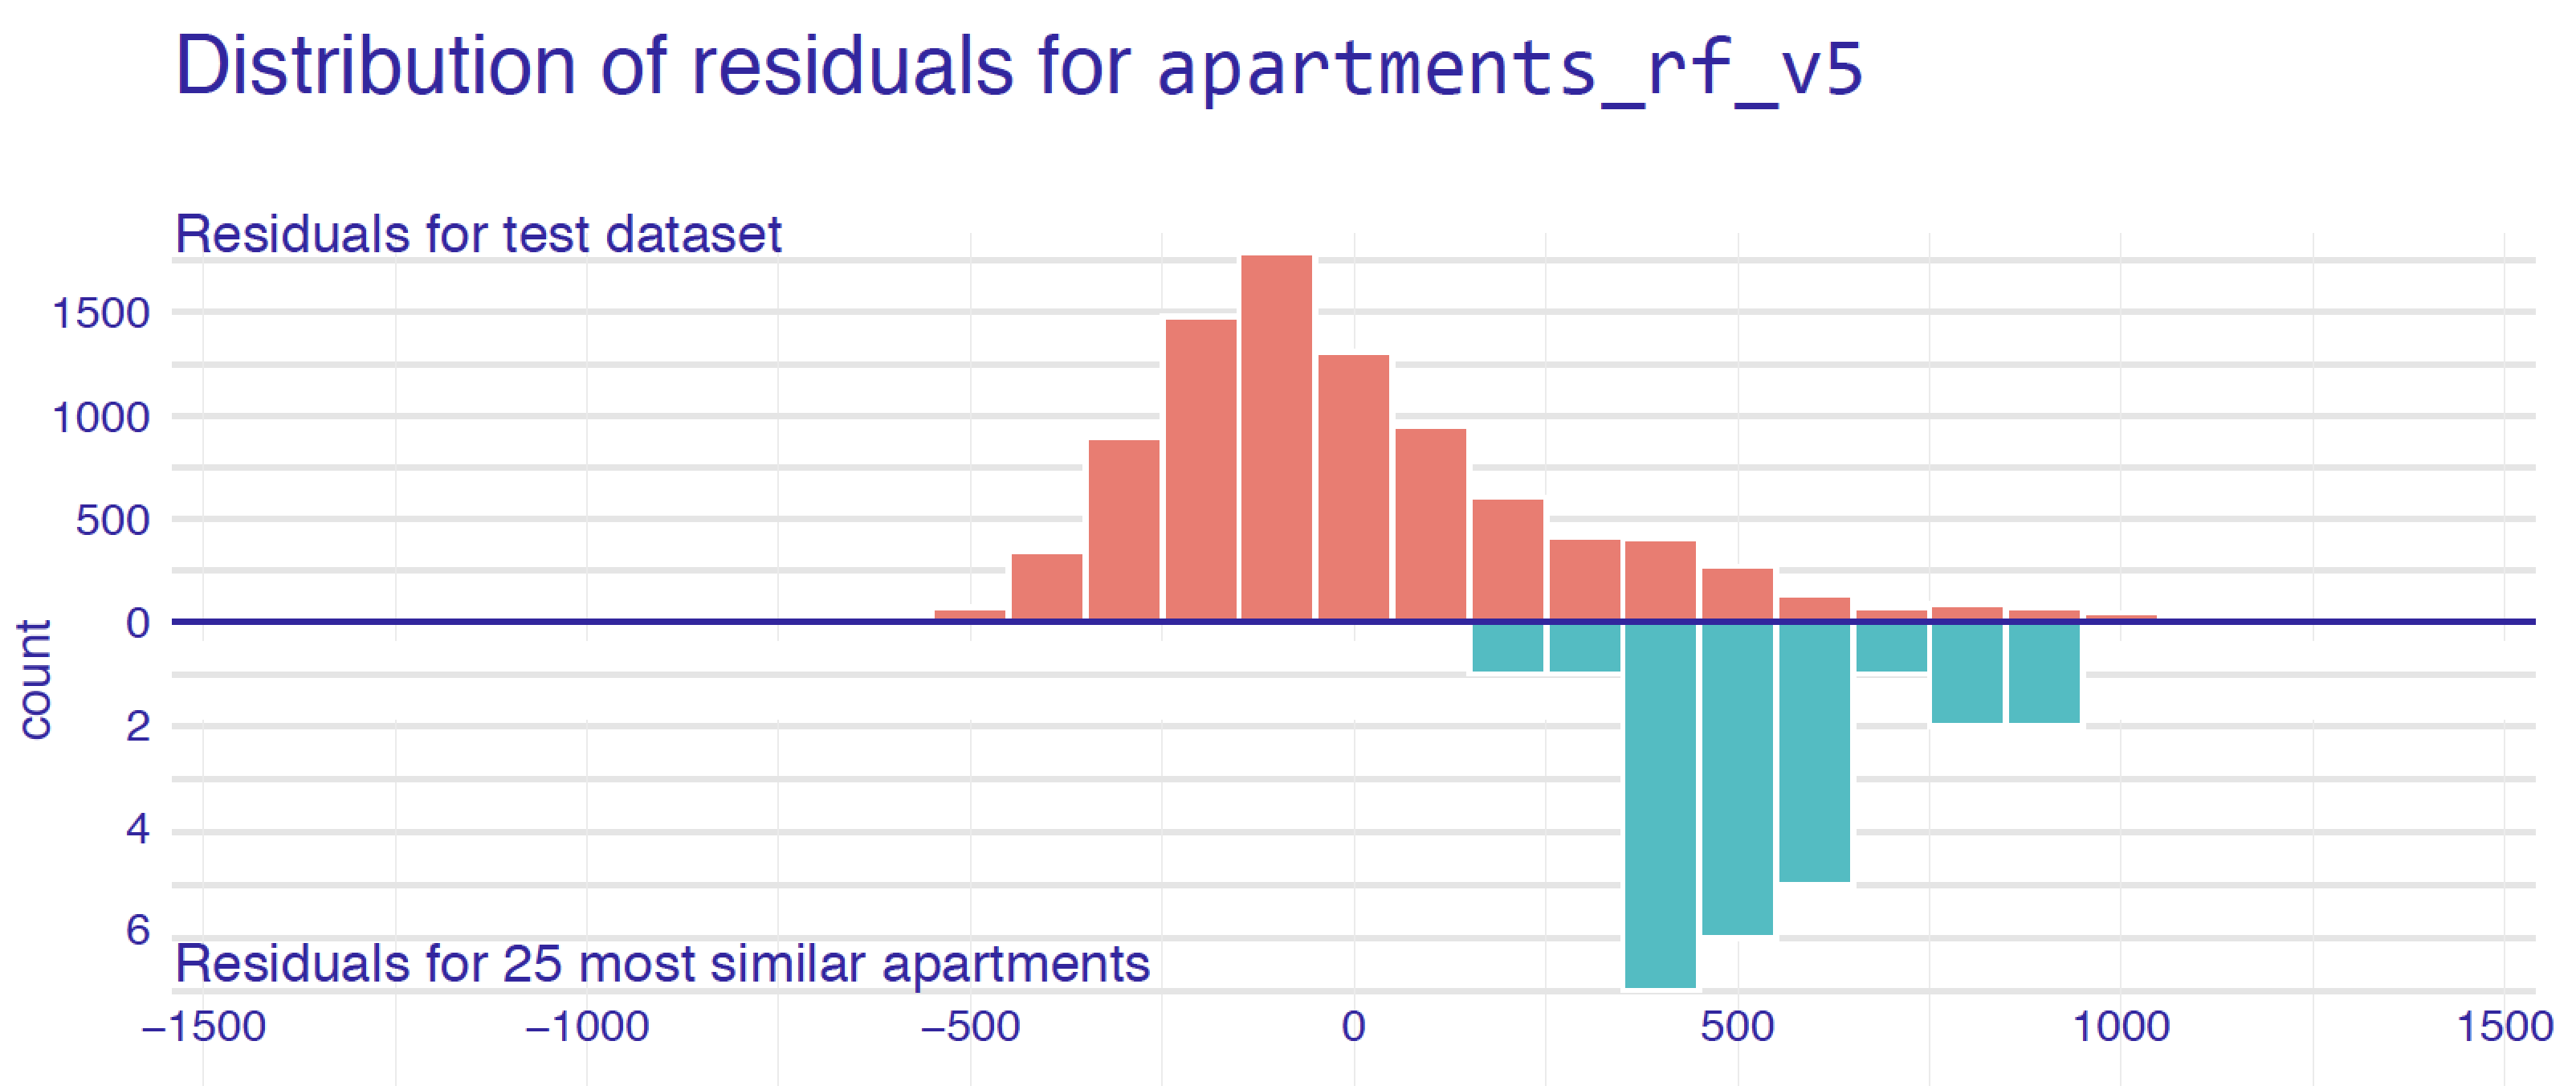
\includegraphics[width=0.7\linewidth]{figure/bb_hist}

\}

\textbackslash{}caption\{(fig:profileBack2BackHist) Histograms of
residuals for the \texttt{apartments\_rf\_v5} model for the Apartments
dataset. Upper panel: residuals calculated for all observations from the
dataset. Bottom panel: residuals calculated for 25 nearest neighbors of
the instance of interest.\}\label{fig:profileBack2BackHist}
\textbackslash{}end\{figure\}

\hypertarget{cPLocDiagMethod}{%
\subsection{Method}\label{cPLocDiagMethod}}

The proposed method is based on three elements:

\begin{itemize}
\tightlist
\item
  identification of nearest neighbors,
\item
  calculation and visualization of CP profiles for the selected
  neighbors, and
\item
  analysis of residuals for the neighbors.
\end{itemize}

In what follows we discuss each of the elements in more detail.

\hypertarget{cPLocDiagNeighbors}{%
\subsubsection{Nearest neighbors}\label{cPLocDiagNeighbors}}

There are two important questions related to the selection of the
neighbors ``nearest'' to the instance (observation) of interest:

\begin{itemize}
\tightlist
\item
  How many neighbors should we choose?
\item
  What metric should be used to measure the ``proximity'' of
  observations?
\end{itemize}

The answer to both questions is, of course, \emph{it depends}.

\begin{itemize}
\tightlist
\item
  The smaller the number of neighbors, the more local is the analysis.
  However, a very small number will lead to a larger variability of the
  results. In many cases we found that 20 neighbors works fine. However,
  one should always take into account computational time (smaller number
  of neighbors results in quicker calculations) and the size of the
  dataset (for a small dataset, smaller sets of neighbors may be
  preferred).
\item
  The metric if very important. The more explanatory variables, the more
  important is the choice. In particular, the metric should be capable
  of accommodating variables of different nature (categorical,
  continuous). Our default choice is the Gower similarity measure:
\end{itemize}

\[
d_{gower}(x_i, x_j) = \frac 1p \sum_{k=1}^p d^k(x_i^k, x_j^k),
\] where \(x_i\) is a \(p\)-dimensional vector of explanatory covariates
for the \(i\)-th observation and \(d^k(x_i^k,x_j^k)\) is the distance
between values of the \(k\)-th variable for the \(i\)-th and \(j\)-th
observations. Note that \(d^k()\) depends on the nature of the variable.
For instance, for a continuous variable it is equal to
\(|x_i^k-x_j^k|/\{max(x_1^k,\ldots,x_n^k)-min(x_1^k,\ldots,x_n^k)\}\),
i.e., the absolute difference scaled by the observed range of the
variable. On the other hand, for a categorical variable, it is simply
\(I(x_i^k = x_j^k)\), where \(I()\) is the indicator function. Note that
\(p\) may be equal to the number of all explanatory variables included
in the model, or only a subset of them.

Once we have decided on the number of neighbors, we can use the chosen
metric to select the required number observations ``closest'' to the one
of interest.

\hypertarget{cPLocDiagProfiles}{%
\subsubsection{Profiles for neighbors}\label{cPLocDiagProfiles}}

Once nearest neighbors have been identified, we can graphically compare
CP profiles for selected (or all) variables.

For a model with a large number of variables, we may end up with a large
number of plots. In such a case a better strategy is to focus only on
\(K\) most important variables, selected by using the
variable-importance measure (see Chapter
\ref{ceterisParibusOscillations}).

\hypertarget{cPLocDiagLFplot}{%
\subsubsection{Local-fidelity plot}\label{cPLocDiagLFplot}}

CP profiles are helpful to assess the model stability. In addition, we
can enhance the plot by adding residuals to it to allow evaluation of
the local model fit. For model \(f()\) and observation \(i\) described
by the vector of explanatory variables \(x_i\), the residual is the
difference between the observed and predicted value of the dependent
variable \(Y_i\), i.e.,

\[
r_i = y_i - f(x_i).
\] Note that, for a binary variable, the residual is the difference
between the value of 0 or 1, depending on how we code ``success,'' and
the value of the predicted probability of ``success.'' This defintion
also applies to categorical responses, as it is common to define, in
such case, a binary ``success'' indicator and compute the predicted
probaiblity of ``success'' for each category separately.

The plot that includes CP profiles for the nearest neighbors and the
corresponding residuals is called a local-fidelity plot.

\hypertarget{cPLocDiagExample}{%
\subsection{Example: Titanic}\label{cPLocDiagExample}}

As an example, we will use the predictions for the random forest model
for the Titanic data (see Section \ref{model-titanic-rf}).

Figure \ref{fig:localFidelityPlots} presents a detailed explanation of
the elements of a local-fidelity plot for \emph{age}, a continuous
explanatory variable. The plot includes eight nearest neighbors of Henry
(see Section \ref{predictions-titanic}). Profiles are quite apart from
each other, which indicates potential instability of model predictions.
However, the residuals included in the plots are positive and negative,
indicating that, on average, the instance prediction should not be
biased.

Figure \ref{fig:localFidelityPlots2} presents a local-fidelity plot for
the categorical explanatory variable \texttt{class}. Henry and his
neighbors traveled in the \texttt{1st} class. In different panels we see
how the predicted probabilityof survival changes if the \texttt{1st}
class is replaced, for instance, by the \texttt{2nd} (in most cases,
they probability will be reduced) or the \texttt{deck\ crew} (in most
cases, the probability will increase). Such plots can help to detect
interactions, as we see that the same change (let's say, from the
\texttt{1st} to the \texttt{3rd} class) results in a different change of
the model prediction.

\begin{figure}

{\centering 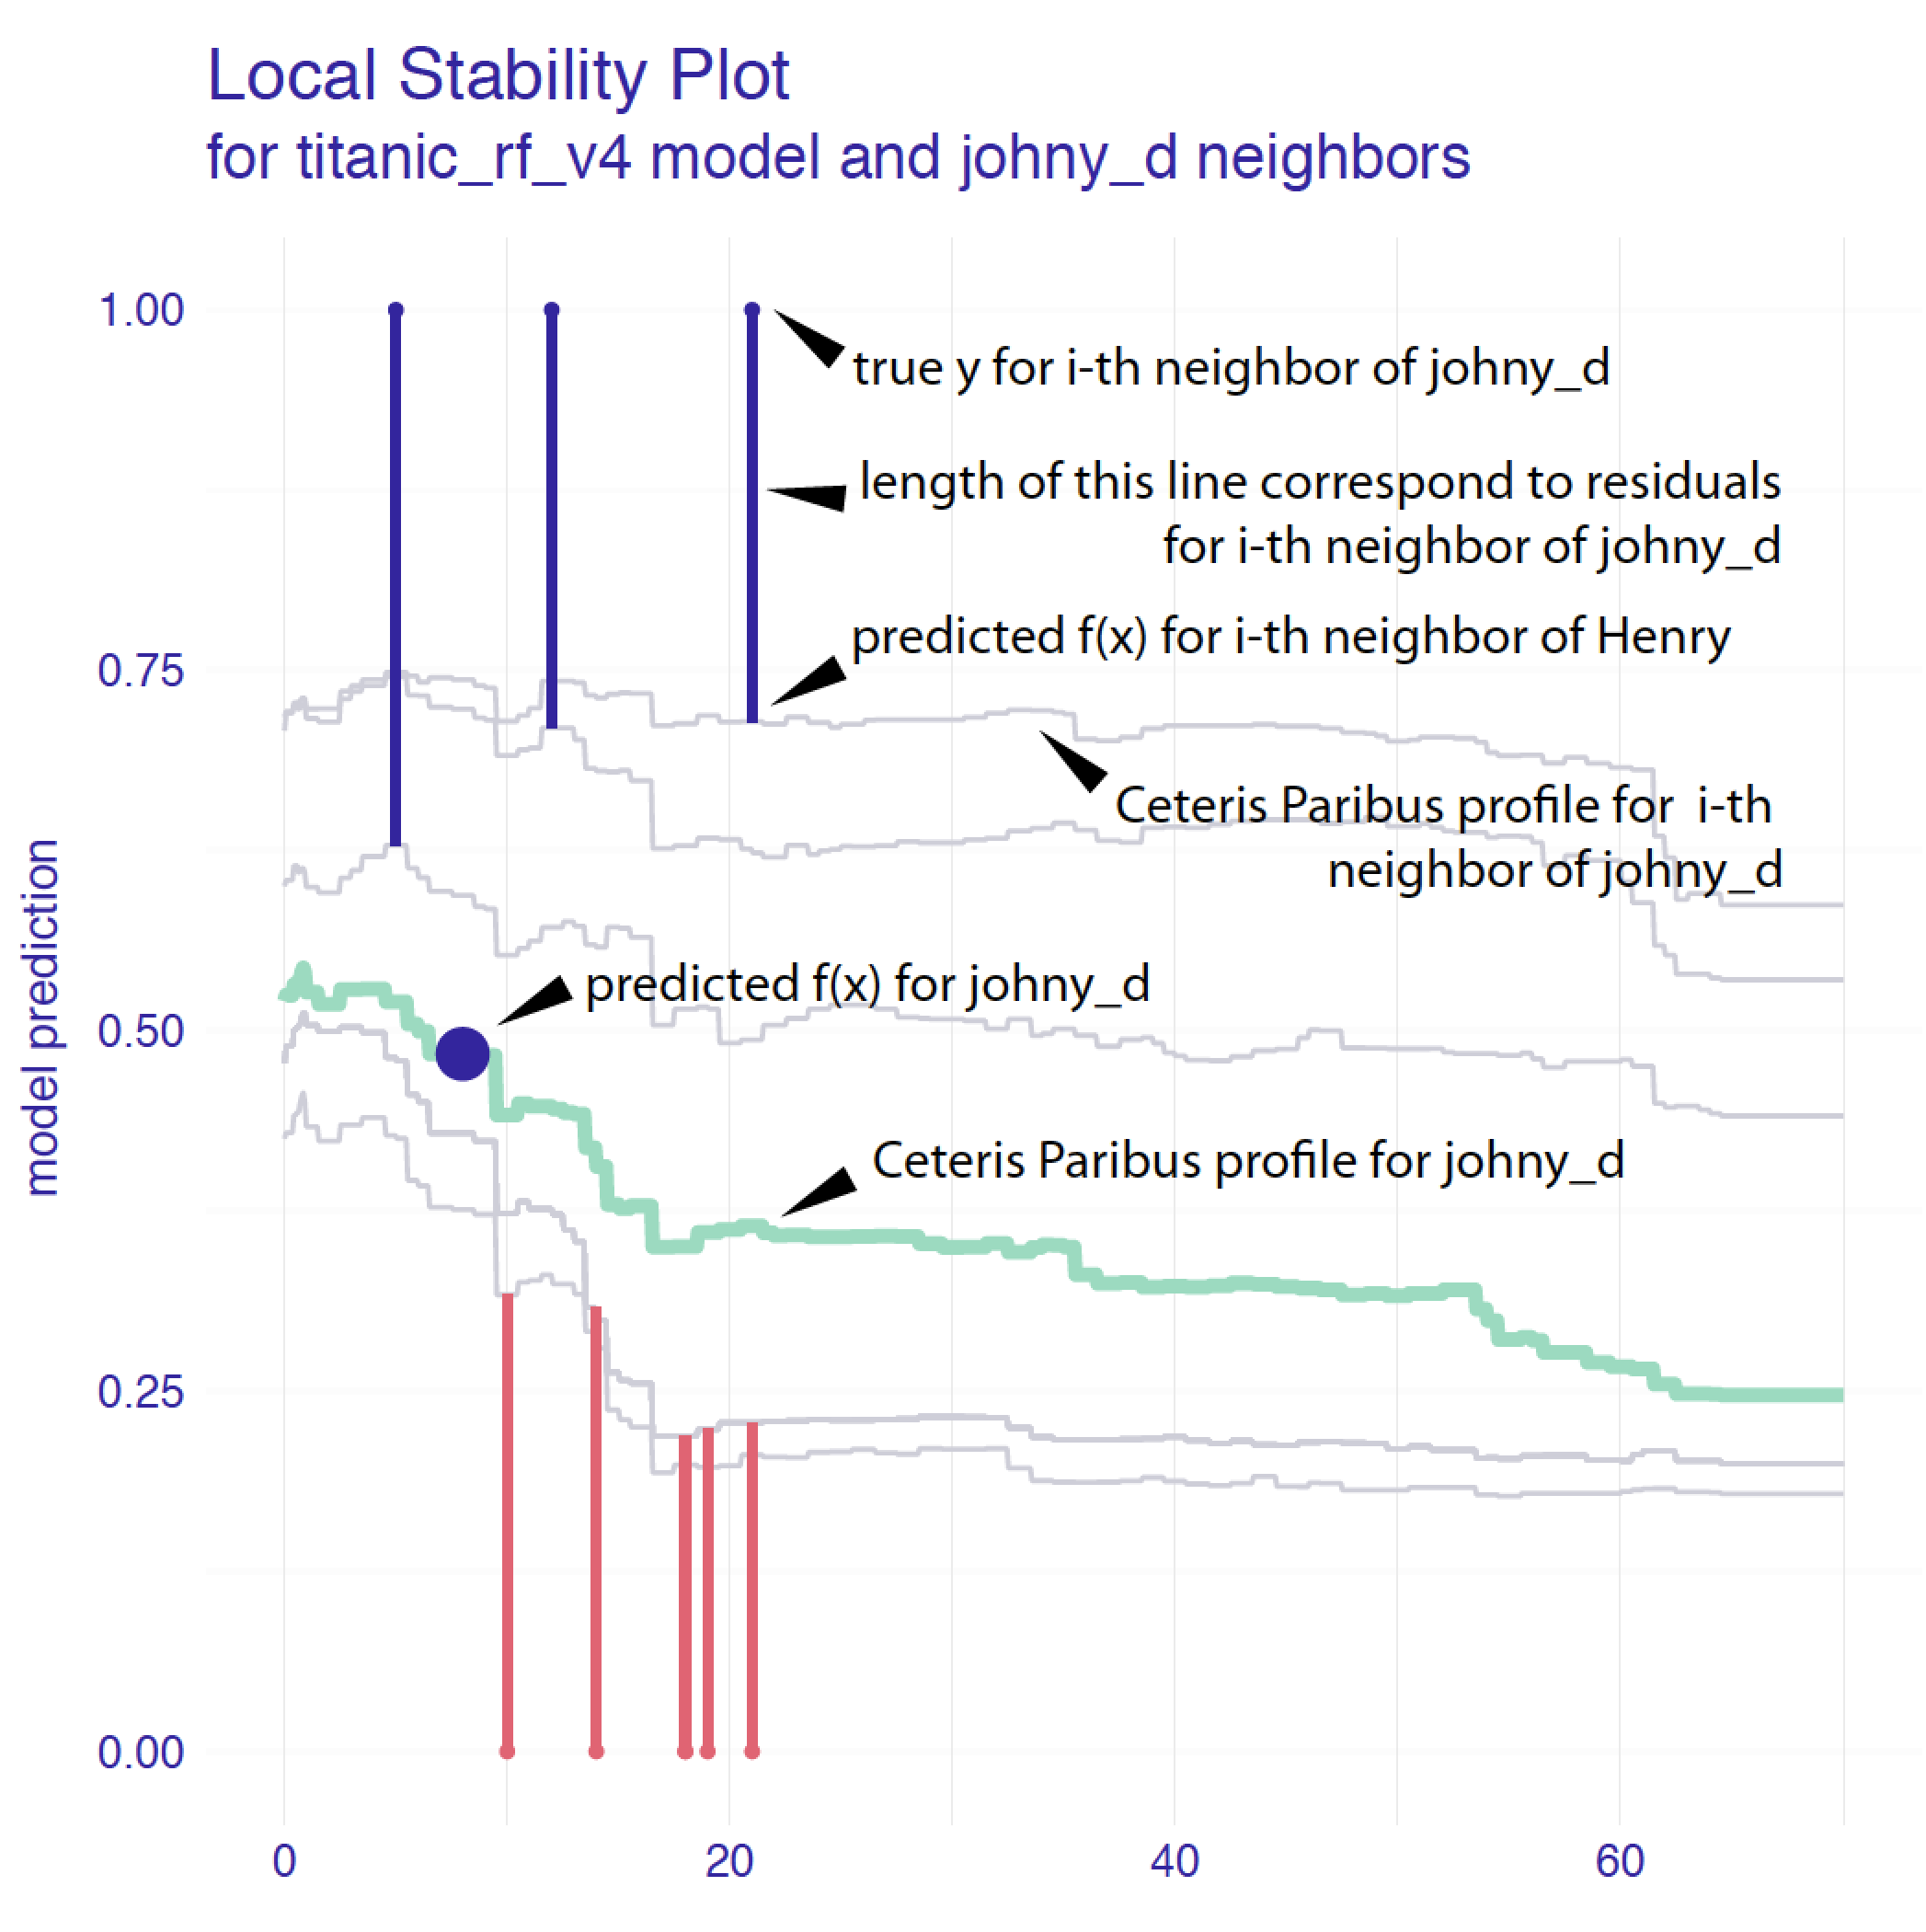
\includegraphics[width=0.7\linewidth]{figure/localFidelityPlots} 

}

\caption{(fig:localFidelityPlots) Elements of a local-fidelity plot for a continuous explanatory variable. The green line shows the Ceteris-paribus profile for the instance of interest. Profiles of the nearest neighbors are marked with grey lines. The vertical intervals correspond to residuals; the shorter the interval, the smaller the residual and the more accurate prediction of the model. Blue intervals correspond to positive residuals, red intervals to negative intervals. Stable model will have profiles close to each other; additive model will have parallel lines.}\label{fig:localFidelityPlots}
\end{figure}

\begin{figure}

{\centering 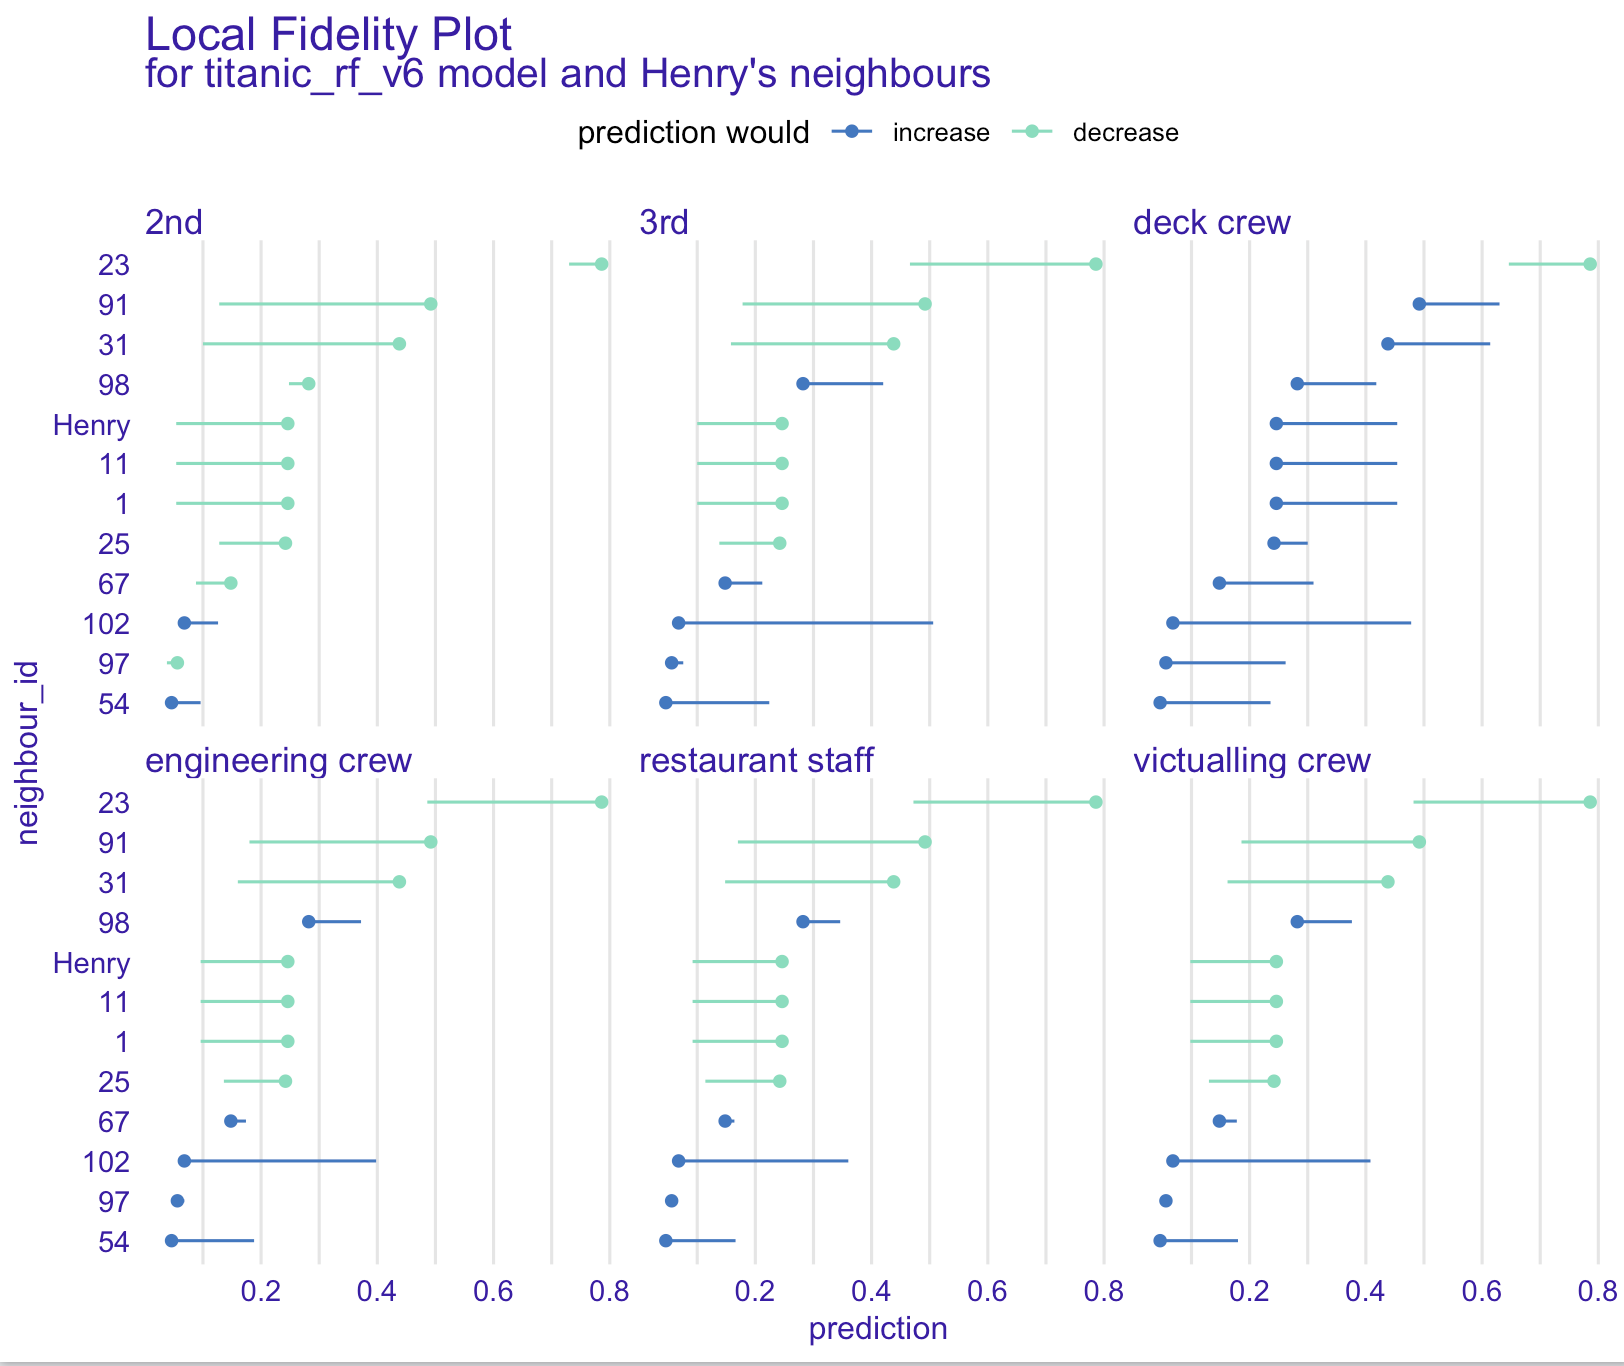
\includegraphics[width=0.7\linewidth]{figure/cp_fidelity_2} 

}

\caption{(fig:localFidelityPlots2) The local-fidelity plot for the categorical explanatory variable `class` in the random effects model for the Titanic data, Henry, and his 10 neighbors. Each panel indicates how the model prediction would change if the class changed from  `1st` to another one. Dots indicate original model predictions for the neighbors; the end of the interval corresponds to model prediction after changing the class. The top-lef panel indicates that, for the majority of the neighbors, the change from the `1st` to the `2nd` class reduces the predicted value of the probability of survival. On the other hand, the top-right panel indicates that changing the lass to `deck crew` members increases the predicted probability.}\label{fig:localFidelityPlots2}
\end{figure}

\hypertarget{cPLocDiagProsCons}{%
\subsection{Pros and cons}\label{cPLocDiagProsCons}}

Local-fidelity plots may be very helpful to check if

\begin{itemize}
\tightlist
\item
  the model is locally additive, as for such models the CP profiles
  should be parallel;
\item
  the model is locally stable, as in that case the CP profiles should be
  close to each other;
\item
  the model fit for the instance of interest is good, as in that case
  the residuals should be small and their distribution should be
  balanced around 0.
\end{itemize}

The drawback is that such plots are quite complex and lack objective
measures of the quality of the model fit. Thus, they are mainly suitable
for an exploratory analysis.

\hypertarget{cPLocDiagR}{%
\subsection{Code snippets for R}\label{cPLocDiagR}}

In this section, we show how to use the R package \texttt{ingredients}
\citep{R-ingredients} to construct local-fidelity plots. More details
and examples can be found at
\texttt{https://modeloriented.github.io/ingredients/}.

We use the random forest model \texttt{titanic\_rf\_v6} developed for
the Titanic dataset (see Section \ref{model-titanic-rf} ) as the
example. Recall that we try to address a classification problem for a
binary dependent variable - we want to predict the probability of
survival for a selected passenger.

\texttt{DALEX} explainers for the model and the \texttt{henry} data
frame are retrieved via \texttt{archivist} hooks, as listed in Section
\ref{ListOfModelsTitanic}.

\begin{Shaded}
\begin{Highlighting}[]
\KeywordTok{library}\NormalTok{(}\StringTok{"randomForest"}\NormalTok{)}
\NormalTok{explain_rf_v6 <-}\StringTok{ }\NormalTok{archivist}\OperatorTok{::}\KeywordTok{aread}\NormalTok{(}\StringTok{"pbiecek/models/9b971"}\NormalTok{)}

\KeywordTok{library}\NormalTok{(}\StringTok{"DALEX"}\NormalTok{)}
\NormalTok{henry <-}\StringTok{ }\NormalTok{archivist}\OperatorTok{::}\KeywordTok{aread}\NormalTok{(}\StringTok{"pbiecek/models/a6538"}\NormalTok{)}
\NormalTok{henry}
\end{Highlighting}
\end{Shaded}

\begin{verbatim}
##   class gender age sibsp parch fare  embarked
## 1   1st   male  47     0     0   25 Cherbourg
\end{verbatim}

We will show how to construct Figure \ref{fig:profileWith10NN}. Toward
this aim we need some number of passengers most similar to
\texttt{henry}. To select the `'neighbors'', we use the
\texttt{select\_neighbours()} function from the \texttt{ingredients}
package. It returns \texttt{n} observations (by default, 20) most
similar to the observation of interest according to the
\texttt{distance} measure (by default, the Gower distance is used).

In the example below, we select 10 nearest neighbors to \texttt{henry}
find from the \texttt{titanic} dataset. Note that the similarity is
based only on two explanatory variables, \emph{gender}, and
\emph{class}, as indicated in the argument \texttt{variables}.

\begin{Shaded}
\begin{Highlighting}[]
\KeywordTok{library}\NormalTok{(}\StringTok{"ingredients"}\NormalTok{)}
\NormalTok{henry_neighbors <-}\StringTok{ }\KeywordTok{select_neighbours}\NormalTok{(titanic, }
\NormalTok{                         henry, }
                         \DataTypeTok{n =} \DecValTok{10}\NormalTok{, }
                         \DataTypeTok{variables =} \KeywordTok{c}\NormalTok{(}\StringTok{"class"}\NormalTok{, }\StringTok{"gender"}\NormalTok{))}
\end{Highlighting}
\end{Shaded}

Now we are ready to plot profiles for Henry and his neighbors. First, we
have got to calculate the corresponding profiles with
\texttt{ceteris\_paribus()} function introduced in Section \ref{CPR}.

\begin{Shaded}
\begin{Highlighting}[]
\NormalTok{cp_henry <-}\StringTok{ }\KeywordTok{ceteris_paribus}\NormalTok{(explain_rf_v6, }
\NormalTok{                            henry,}
                            \DataTypeTok{variable_splits =} \KeywordTok{list}\NormalTok{(}\DataTypeTok{age =} \KeywordTok{seq}\NormalTok{(}\DecValTok{0}\NormalTok{,}\DecValTok{80}\NormalTok{,}\FloatTok{0.1}\NormalTok{)))}
\NormalTok{cp_henry_neighbors <-}\StringTok{ }\KeywordTok{ceteris_paribus}\NormalTok{(explain_rf_v6, }
\NormalTok{                            henry_neighbors,}
                            \DataTypeTok{variable_splits =} \KeywordTok{list}\NormalTok{(}\DataTypeTok{age =} \KeywordTok{seq}\NormalTok{(}\DecValTok{0}\NormalTok{,}\DecValTok{80}\NormalTok{,}\FloatTok{0.1}\NormalTok{)))}
\end{Highlighting}
\end{Shaded}

Subsequently, we can plot the profiles. Note that, in the example below,
we do this only for a single variable \texttt{age}.

\begin{Shaded}
\begin{Highlighting}[]
\KeywordTok{library}\NormalTok{(}\StringTok{"ggplot2"}\NormalTok{)}

\KeywordTok{plot}\NormalTok{(cp_henry_neighbors, }\DataTypeTok{color =} \StringTok{'#ceced9'}\NormalTok{) }\OperatorTok{+}
\CommentTok{#  show_profiles(cp_henry, size = 2)  +}
\StringTok{  }\KeywordTok{ggtitle}\NormalTok{(}\StringTok{"Ceteris-paribus profiles for Henry and neighbors"}\NormalTok{, }\StringTok{"Calculated for the titanic_rf_v6 model"}\NormalTok{)}
\end{Highlighting}
\end{Shaded}

\begin{center}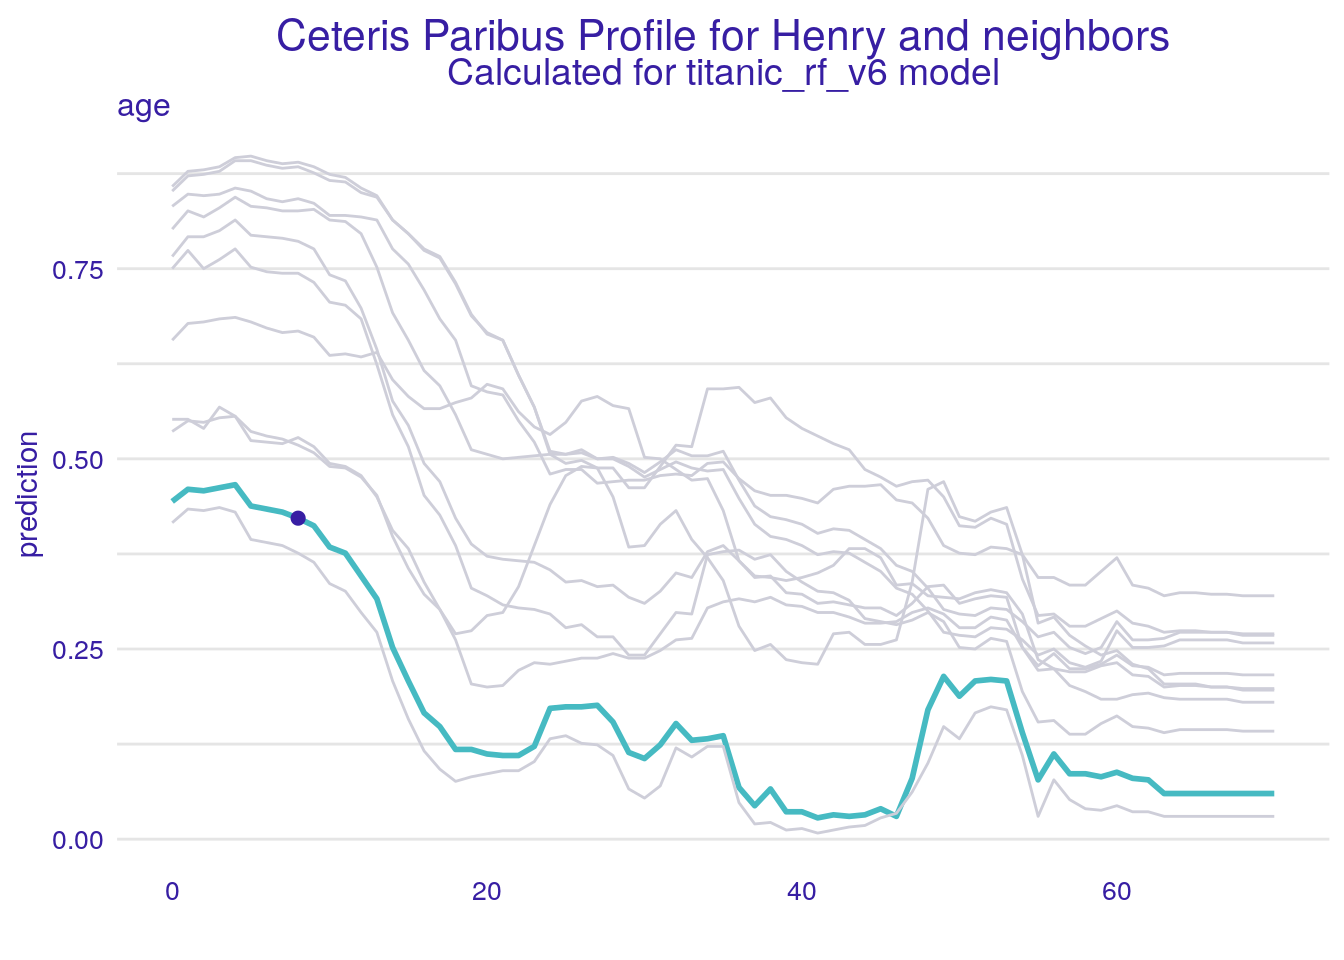
\includegraphics[width=0.7\linewidth]{PM_VEE_files/figure-latex/titanicCeterisParibus05-1} \end{center}

To construct the local-fidelity plot presented in Figure
\ref{fig:localFidelityPlots}, we have got to add the information about
the observed values of the dependent variable for the selected
neighbors. Toward this aim, we use the \texttt{y} argument in the
\texttt{ceteris\_paribus()} function. The argument takes numerical
values. Our binary dependent variable \texttt{survived} assumes values
\texttt{yes/no}; to convert them to numerical values, we use the
\texttt{survived\ ==\ "yes"} expression.

\begin{Shaded}
\begin{Highlighting}[]
\NormalTok{cp_henry_neighbors <-}\StringTok{ }\KeywordTok{ceteris_paribus}\NormalTok{(explain_rf_v6,}
\NormalTok{                          henry_neighbors, }
                          \DataTypeTok{y =}\NormalTok{ henry_neighbors}\OperatorTok{$}\NormalTok{survived }\OperatorTok{==}\StringTok{ "yes"}\NormalTok{,}
                          \DataTypeTok{variable_splits =} \KeywordTok{list}\NormalTok{(}\DataTypeTok{age =} \KeywordTok{seq}\NormalTok{(}\DecValTok{0}\NormalTok{,}\DecValTok{80}\NormalTok{,}\FloatTok{0.1}\NormalTok{)))}
\end{Highlighting}
\end{Shaded}

Finally, we add residuals to the plot by using the
\texttt{show\_residuals()} function. As a result, we obtain the
local-fidelity plot for \texttt{henry}.

\begin{Shaded}
\begin{Highlighting}[]
\KeywordTok{plot}\NormalTok{(cp_henry_neighbors, }\DataTypeTok{color =} \StringTok{'#ceced9'}\NormalTok{) }\OperatorTok{+}
\CommentTok{#  show_profiles(cp_henry, size = 2) + }
\StringTok{  }\KeywordTok{show_observations}\NormalTok{(cp_henry, }\DataTypeTok{variables =} \StringTok{"age"}\NormalTok{, }\DataTypeTok{size =} \DecValTok{5}\NormalTok{) }\OperatorTok{+}
\CommentTok{#  show_residuals(cp_henry_neighbors, variables = "age") +}
\StringTok{  }\KeywordTok{ggtitle}\NormalTok{(}\StringTok{"Local-fidelity plot for Henry"}\NormalTok{,}\StringTok{"Calculated for the titanic_rf_v6 model"}\NormalTok{)}
\end{Highlighting}
\end{Shaded}

\begin{center}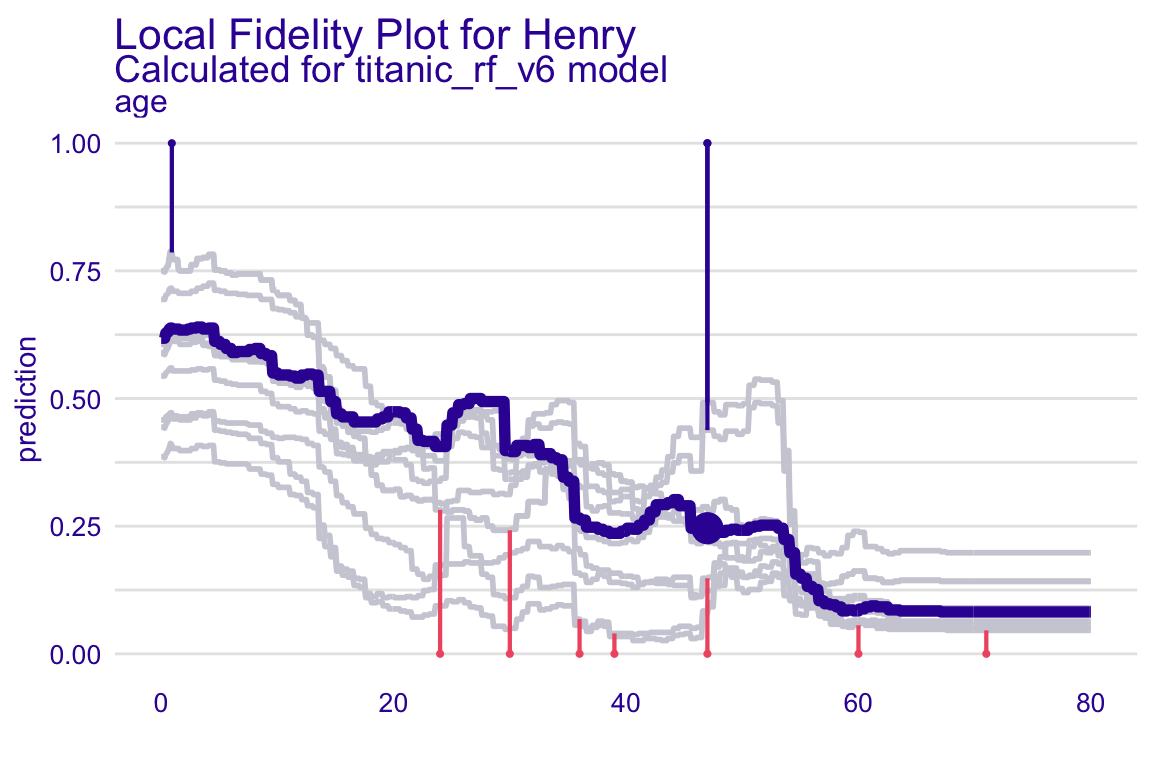
\includegraphics[width=0.7\linewidth]{PM_VEE_files/figure-latex/titanicCeterisParibus07-1} \end{center}

\hypertarget{breakDown}{%
\section{Break Down for Additive Variable
Attributions}\label{breakDown}}

In the Section \ref{ceterisParibusOscillations} we introduced a method
for assessment of local variable importance based on Ceteris Paribus
Profiles. But the main disadvantage of this method is that importance
scores do not sum up to final model predictions.

In this chapter we introduce Break Down Plots which solve this problem.
Note that the described method is also similar to the EXPLAIN algorithm
introduced in \citep{explainPaper} and implemented in
\citep{explainPackage} package.

\hypertarget{intuition}{%
\subsection{Intuition}\label{intuition}}

For any model we may repeat the intuition presented in the Section
\ref{variableAttributionMethods} to calculate variable contribution as
shifts in expected model response after conditioning over consecutive
variables. This intuition is presented in Figure \ref{fig:BDPrice4}.

Panel A shows distribution of model responses. The row
\texttt{all\ data} shows the model response of the validation dataset.
The red dot stands for average model response and it is an estimate of
expected model response \(E [f(x)]\).

Since we want to calculate effects of particular values of selected
variables we then condition over these variables in a sequential manner.
The next row in panel A corresponds to average model prediction for
observations with variable \texttt{class} fixed to value \texttt{1st}.
The next for corresponds to average model prediction with variables
\texttt{class} set to \texttt{1st} and \texttt{age} set to \texttt{0},
and so on. The last row corresponds to model response for \(x_*\).

Black lines in the panel A show how prediction for a single point
changes after coordinate \(j\) is replaced by the \(x_*^j\), so they
span between \(f(x)\) and \(f(x^{j|=x_*^j})\). But finally we are not
interested in particular changes, not even in distributions but only in
averages - expected model responses.

The most minimal form that shows important information is presented in
the panel C. Positive values are presented with green bars while
negative differences are marked with red bar. They sum up to final model
prediction, which is denoted by a violet bar in this example.

\begin{figure}

{\centering 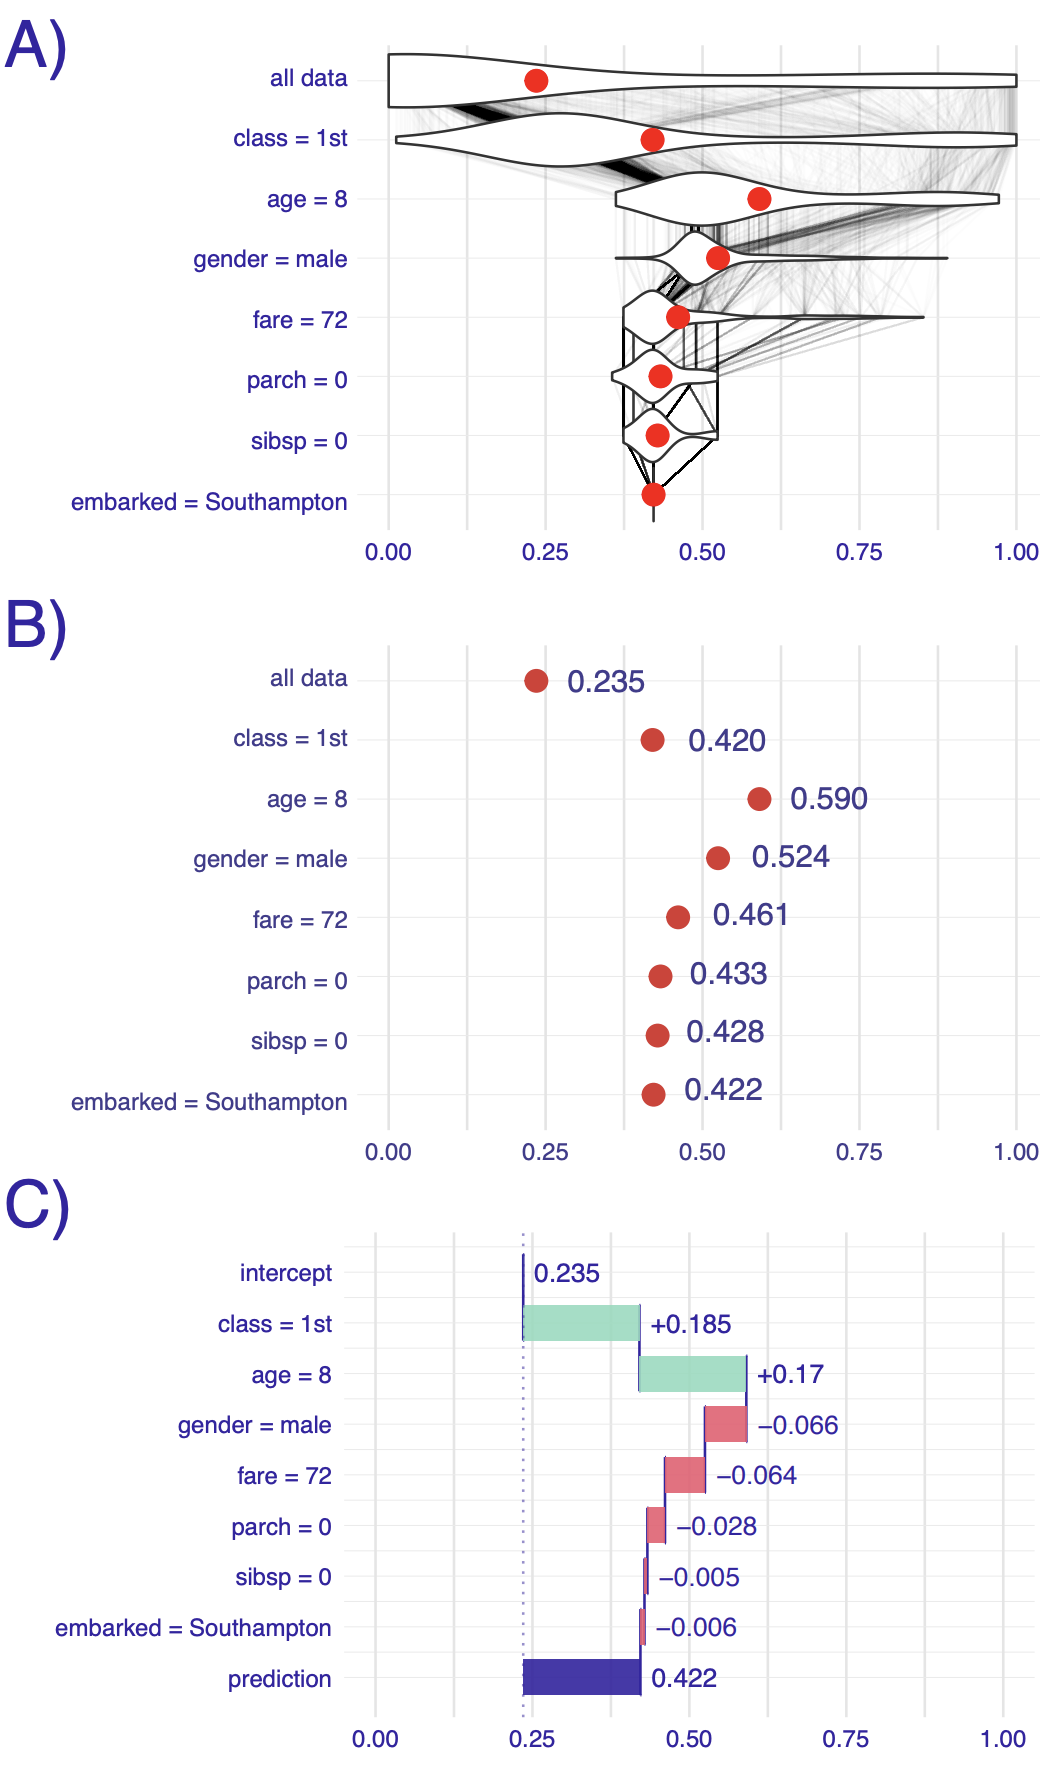
\includegraphics[width=0.8\linewidth]{figure/break_down_distr} 

}

\caption{(fig:BDPrice4) Break Down Plots show how variables move the model prediction from population average to the model prognosis for a single observation. A) The first row shows distribution of model predictions. Next rows show conditional distributions, every row a new variable is added to conditioning. The last row shows model prediction for a single point. Red dots stand for averages. B) Red dots stands for average conditional model response. C) Only variable contributions are presented, i.e. differences between consecutive conditional expectations. }\label{fig:BDPrice4}
\end{figure}

\hypertarget{method}{%
\subsection{Method}\label{method}}

Again, as in previous chapter, let \(v(j, x_*)\) stands for the
contribution of variable \(j\) to prediction of model \(f\) in point
\(x_*\).

We expect that such contribution will sum up to the model prediction in
a given point (property called \emph{local accuracy}), so \[
f(x_*) = v_0 + \sum_{j=1}^p v(j, x_*)
\] where \(v_0\) stands for average model response (it may be different
for different models).

Note that the equation above may be rewritten as

\[
E [f(X)|X^1 = x^1_*, \ldots, X^p = x^p_*] = E[f(X)] + \sum_{j=1}^p v(j, x_*)
\] what leads to quite natural proposition for \(v(j, x_*)\), such as

\[
v(j, x_*) = E [f(X) | X^1 = x^1_*, \ldots, X^j = x^j_*] - E [f(X) | X^1 = x^1_*, \ldots, X^{j-1} = x^{j-1}_*] 
\] In other words the contribution of variable \(j\) is the difference
between expected model response conditioned on first \(i\) variables
minus the model response conditioned on first \(j-1\) variables.

To simplify notation, let's define a symbol \(\Delta^{i|J}\) as \[
\Delta^{i|J} = E [f(X) | X^{J \cup \{i\}} = x^{J \cup \{i\}}_*] - E [f(X) | X^{J} = x^{J}_*],
\] So \(\Delta^{i|J}\) is the change between expectation over variables
from the set \(J \cup \{i\}\) minus expectation over variables from the
set \(J\).

Then

\[
v(j, x_*) = \Delta^{j|\{1,  ..., j-1\}}.
\]

Such proposition fulfills the \emph{local accuracy} condition.

Unfortunately, for non-additive models, variable contributions depend on
the ordering of variables. See for example Figure \ref{fig:ordering}. In
the first ordering the contribution of variable \texttt{age} is
calculated as 0.01, while in the second the contribution is calculated
as 0.13. Such differences are related to the lack of additivness of the
model \(f()\).

\begin{figure}

{\centering 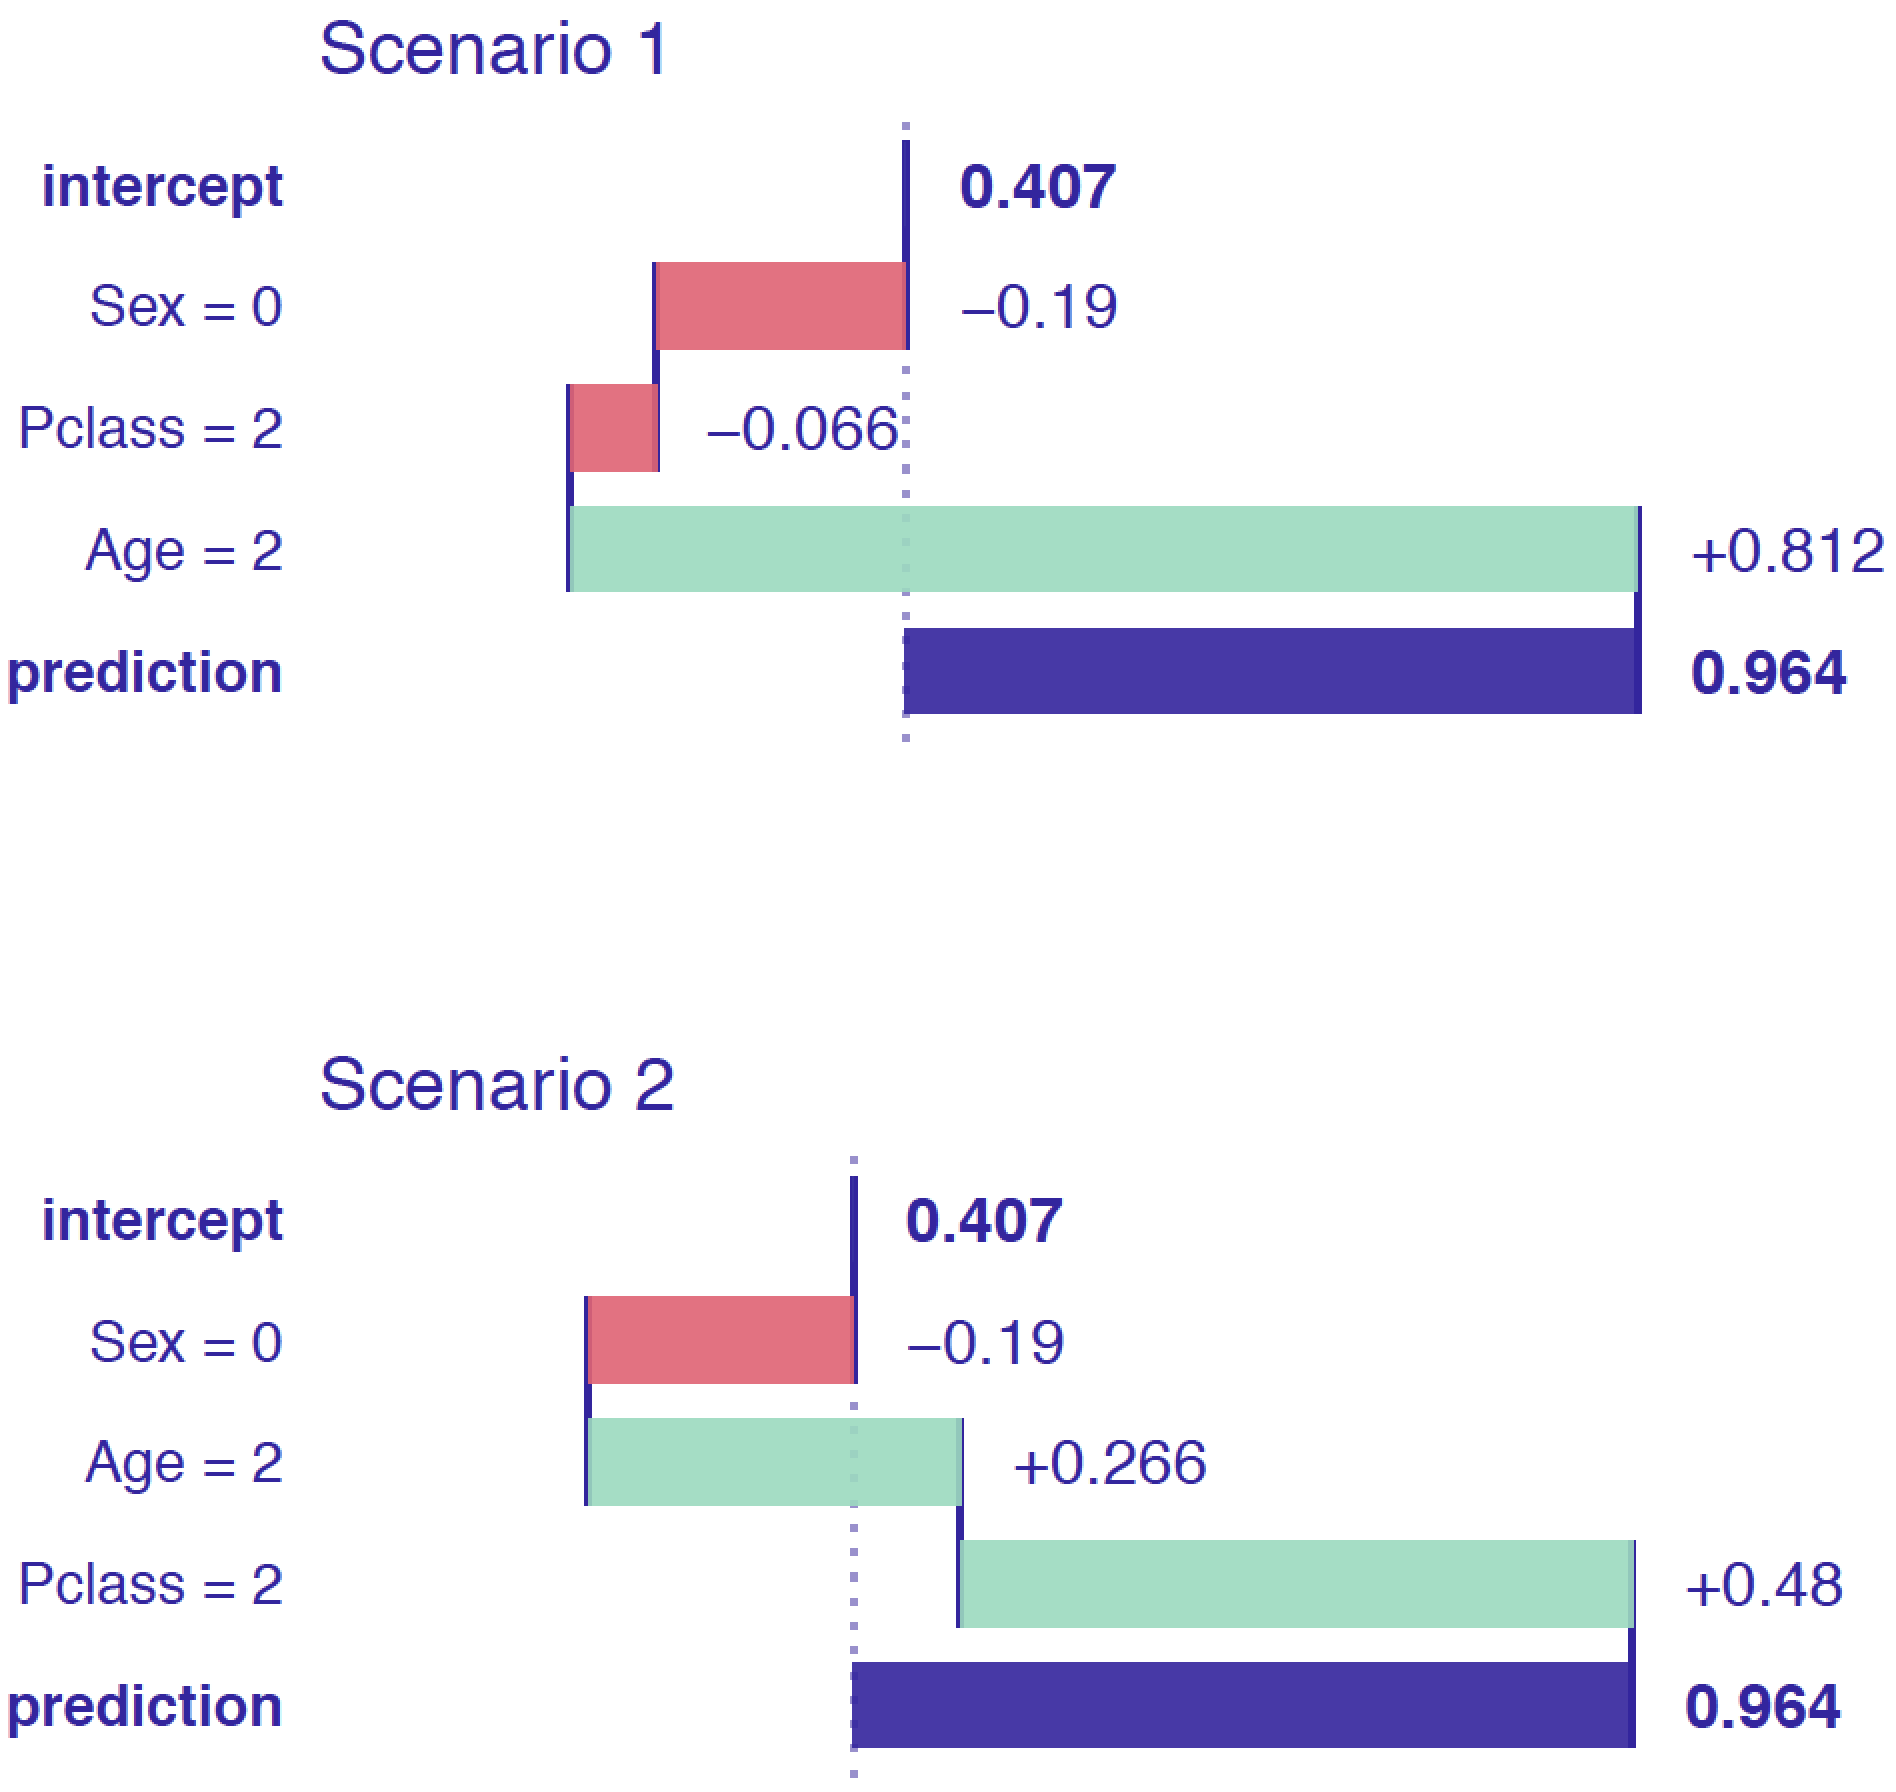
\includegraphics[width=1\linewidth]{figure/ordering} 

}

\caption{(fig:ordering) Two different paths between average model prediction and the model prediction for a selected observation. Black dots stand for conditional average, red arrows stands for changes between conditional averages.}\label{fig:ordering}
\end{figure}

There are different attempts to solve the problem with the ordering.

A. choose an ordering in which variables with largest contributions are
first. In this chapter we will describe a heuristic behind this
approach. B. identify interactions that causes difference in
attributions for different orderings and show these interactions. In the
chapter \ref{iBreakDown} we will describe a heuristic behind this idea.
C. calculate average across all possible orderings. There is \(p!\)
possible orderings, be the may quite accurately approximate the average.
This approach will be presented in the chapter \ref{shapley}.

So, let's start with approach A. The easiest way to solve this problem
is to use two-step procedure. In the first step variables are ordered
and in the second step the consecutive conditioning is applied to
ordered variables.

First step of this algorithm is to determine the order of variables for
conditioning. It seems to be reasonable to include first variables that
are likely to be most important, leaving the noise variables at the end.
This leads to order based on following scores

\[
\Delta^j = \left| E [f(X)] - E [f(X)|X^j = x_*^j] \right|
\] Note, that the absolute value is needed as variable contributions can
be both positive and negative.

Once the ordering is determined in the second step variable
contributions are calculated as

\[
v(j, x_*) = E [f(X) | X^{J \cup \{i\}} = x^{J \cup \{i\}}_*] - E [f(X) | X^{J} = x^{J}_*]  = \Delta ^{i|J}
\] where \(J\) is the set of variables that have scores \(\Delta^i\)
smaller than score for variable \(i\).

\[
J = \{j: \Delta^{j} < \Delta^{i}\}
\]

The time complexity of the first step is \(O(p)\) where \(p\) is the
number of variables and the time complexity of the second step is also
\(O(p)\).

\hypertarget{example-titanic}{%
\subsection{Example: Titanic}\label{example-titanic}}

Let us consider a random forest model \texttt{titanic\_rf\_v6} and the
passenger \texttt{johny\_d} as defined in section
\ref{ListOfModelsTitanic}.

Average model response for all passengers for this model is
\(v_0 = 0.2356585\). For each coordinate of \texttt{johny\_d} we can
calculate scores \(\Delta^j\) and they are presented in the table
\ref{tab:titanicBreakDownDeltas}. These scores determine the order in
which we do the conditioning.

\begin{longtable}[]{@{}lrr@{}}
\caption{\label{tab:titanicBreakDownDeltas} For each variable we calculated
scores \(\Delta^j\). These scores are sorted in the decreasing
order.}\tabularnewline
\toprule
variable \(j\) & \(E[f(X : x^j = x^j_*)]\) & \(\Delta^j\)\tabularnewline
\midrule
\endfirsthead
\toprule
variable \(j\) & \(E[f(X : x^j = x^j_*)]\) & \(\Delta^j\)\tabularnewline
\midrule
\endhead
age & 0.7407795 & 0.5051210\tabularnewline
class & 0.6561034 & 0.4204449\tabularnewline
fare & 0.6141968 & 0.3785383\tabularnewline
sibsp & 0.4786182 & 0.2429597\tabularnewline
parch & 0.4679240 & 0.2322655\tabularnewline
embarked & 0.4602620 & 0.2246035\tabularnewline
gender & 0.3459458 & 0.1102873\tabularnewline
\bottomrule
\end{longtable}

Once the order is determined we can calculate sequential contributions
\(\Delta^{i|J}\). For \texttt{johny\_d} and the model unde
consideration, these coefficients are listed in Table
\ref{tab:titanicBreakDownDeltasConseq}.

\begin{longtable}[]{@{}lrr@{}}
\caption{\label{tab:titanicBreakDownDeltasConseq} Following order defined by
\(\Delta^i\) we calculate sequential conditioning
\(E[f(X|x^I = x^I_*)]\) where \(I\) is an increasing set of already
considered coefficients.}\tabularnewline
\toprule
variable \(i\) & \(E[f(X : x^I = x^I_*)]\) &
\(\Delta^{i|J}\)\tabularnewline
\midrule
\endfirsthead
\toprule
variable \(i\) & \(E[f(X : x^I = x^I_*)]\) &
\(\Delta^{i|J}\)\tabularnewline
\midrule
\endhead
intercept & 0.2353095 & 0.2353095\tabularnewline
age = 8 & 0.5051210 & 0.2698115\tabularnewline
class = 1st & 0.5906969 & 0.0855759\tabularnewline
fare = 72 & 0.5443561 & -0.0463407\tabularnewline
gender = male & 0.4611518 & -0.0832043\tabularnewline
embarked = Southampton & 0.4584422 & -0.0027096\tabularnewline
sibsp = 0 & 0.4523398 & -0.0061024\tabularnewline
parch = 0 & 0.4220000 & -0.0303398\tabularnewline
prediction & 0.4220000 & 0.4220000\tabularnewline
\bottomrule
\end{longtable}

These results can be visually presented with waterfall plot as in the
Figure \ref{fig:BDjohnyExample}.

\textbackslash{}begin\{figure\}

\{\centering 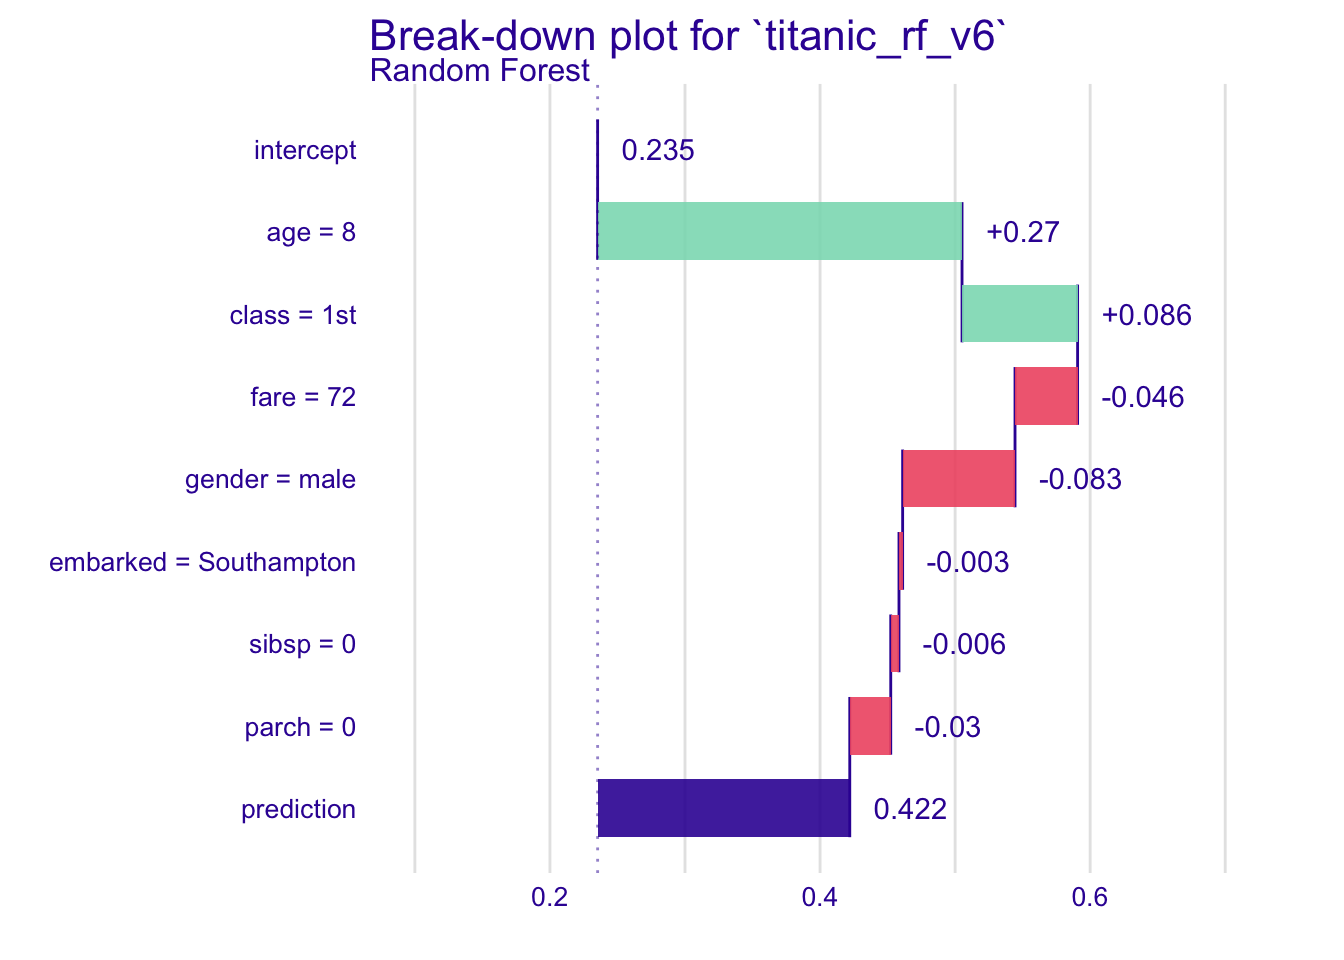
\includegraphics[width=0.99\linewidth]{PM_VEE_files/figure-latex/BDjohnyExample-1}

\}

\textbackslash{}caption\{(fig:BDjohnyExample) Break Down explanations
for the \texttt{titanic\_rf\_v6} model and \texttt{johny\_d}
passanger.\}\label{fig:BDjohnyExample} \textbackslash{}end\{figure\}

\hypertarget{pros-and-cons}{%
\subsection{Pros and cons}\label{pros-and-cons}}

Break Down approach is model agnostic, can be applied to any predictive
model that returns a single number. It leads to additive variable
attribution. Below we summarize key strengths and weaknesses of this
approach.

\textbf{Pros}

\begin{itemize}
\tightlist
\item
  Break Down Plots are easy to understand and decipher.
\item
  Break Down Plots are compact; many variables may be presented in a
  small space.
\item
  Break Down Plots are model agnostic yet they reduce to intuitive
  interpretation for linear Gaussian and generalized models.
\item
  Complexity of Break Down Algorithm is linear in respect to the number
  of variables.
\end{itemize}

\textbf{Cons}

\begin{itemize}
\tightlist
\item
  If the model is non-additive then showing only additive contributions
  may be misleading.
\item
  Selection of the ordering based on scores is subjective. Different
  orderings may lead to different contributions.
\item
  For large number of variables the Break Down Plot may be messy with
  many variables having small contributions.
\end{itemize}

\hypertarget{code-snippets-for-r}{%
\subsection{Code snippets for R}\label{code-snippets-for-r}}

In this section we present key features of the \texttt{iBreakDown}
package for R \citep{iBreakDownRPackage} which is a part of
\texttt{DrWhy.AI} universe. This package covers all features presented
in this chapter. It is available on CRAN and GitHub. Find more examples
at the website of this package
\texttt{https://modeloriented.github.io/iBreakDown/}.

In this section, we use a random forest classification model developed
in the chapter \ref{TitanicDataset}, namely the \texttt{titanic\_rf\_v6}
model. It is trained to predict probability of survival from sinking of
Titanic. Instance level explanations are calculated for a single
observation \texttt{johny\_d} - 8 years old passenger that travels 1st
class.

\texttt{DALEX} explainers for both models and the Henry data are
retrieved via \texttt{archivist} hooks as listed in Chapter
\ref{ListOfModelsTitanic}.

\begin{Shaded}
\begin{Highlighting}[]
\KeywordTok{library}\NormalTok{(}\StringTok{"randomForest"}\NormalTok{)}
\NormalTok{explain_rf_v6 <-}\StringTok{ }\NormalTok{archivist}\OperatorTok{::}\KeywordTok{aread}\NormalTok{(}\StringTok{"pbiecek/models/9b971"}\NormalTok{)}

\KeywordTok{library}\NormalTok{(}\StringTok{"DALEX"}\NormalTok{)}
\NormalTok{johny_d <-}\StringTok{ }\NormalTok{archivist}\OperatorTok{::}\KeywordTok{aread}\NormalTok{(}\StringTok{"pbiecek/models/e3596"}\NormalTok{)}
\NormalTok{johny_d}
\end{Highlighting}
\end{Shaded}

\hypertarget{basic-usage-for-the-break_down-function}{%
\subsubsection{\texorpdfstring{Basic usage for the \texttt{break\_down}
function}{Basic usage for the break\_down function}}\label{basic-usage-for-the-break_down-function}}

The \texttt{iBreakDown::break\_down()} function calculates Break Down
contributions for a selected model around a selected observation.

The result from \texttt{break\_down()} function is a data frame with
additive attributions for selected observation.

The simplest use case is to set only the arguments - model explainers
and observation of interest.

Note that the table below recreates values presented in Table
\ref{tab:titanicBreakDownDeltasConseq}.

\begin{Shaded}
\begin{Highlighting}[]
\KeywordTok{library}\NormalTok{(}\StringTok{"iBreakDown"}\NormalTok{)}
\NormalTok{bd_rf <-}\StringTok{ }\KeywordTok{break_down}\NormalTok{(explain_rf_v6,}
\NormalTok{                 johny_d)}
\NormalTok{bd_rf}
\end{Highlighting}
\end{Shaded}

\begin{verbatim}
##                                          contribution
## Random Forest v6: intercept                     0.235
## Random Forest v6: age = 8                       0.270
## Random Forest v6: class = 1st                   0.086
## Random Forest v6: fare = 72                    -0.046
## Random Forest v6: gender = male                -0.083
## Random Forest v6: embarked = Southampton       -0.003
## Random Forest v6: sibsp = 0                    -0.006
## Random Forest v6: parch = 0                    -0.030
## Random Forest v6: prediction                    0.422
\end{verbatim}

The generic \texttt{plot()} function creates Break Down plots.

Note that the plot below recreates Figure \ref{fig:BDjohnyExample}.

\begin{Shaded}
\begin{Highlighting}[]
\KeywordTok{plot}\NormalTok{(bd_rf) }
\end{Highlighting}
\end{Shaded}

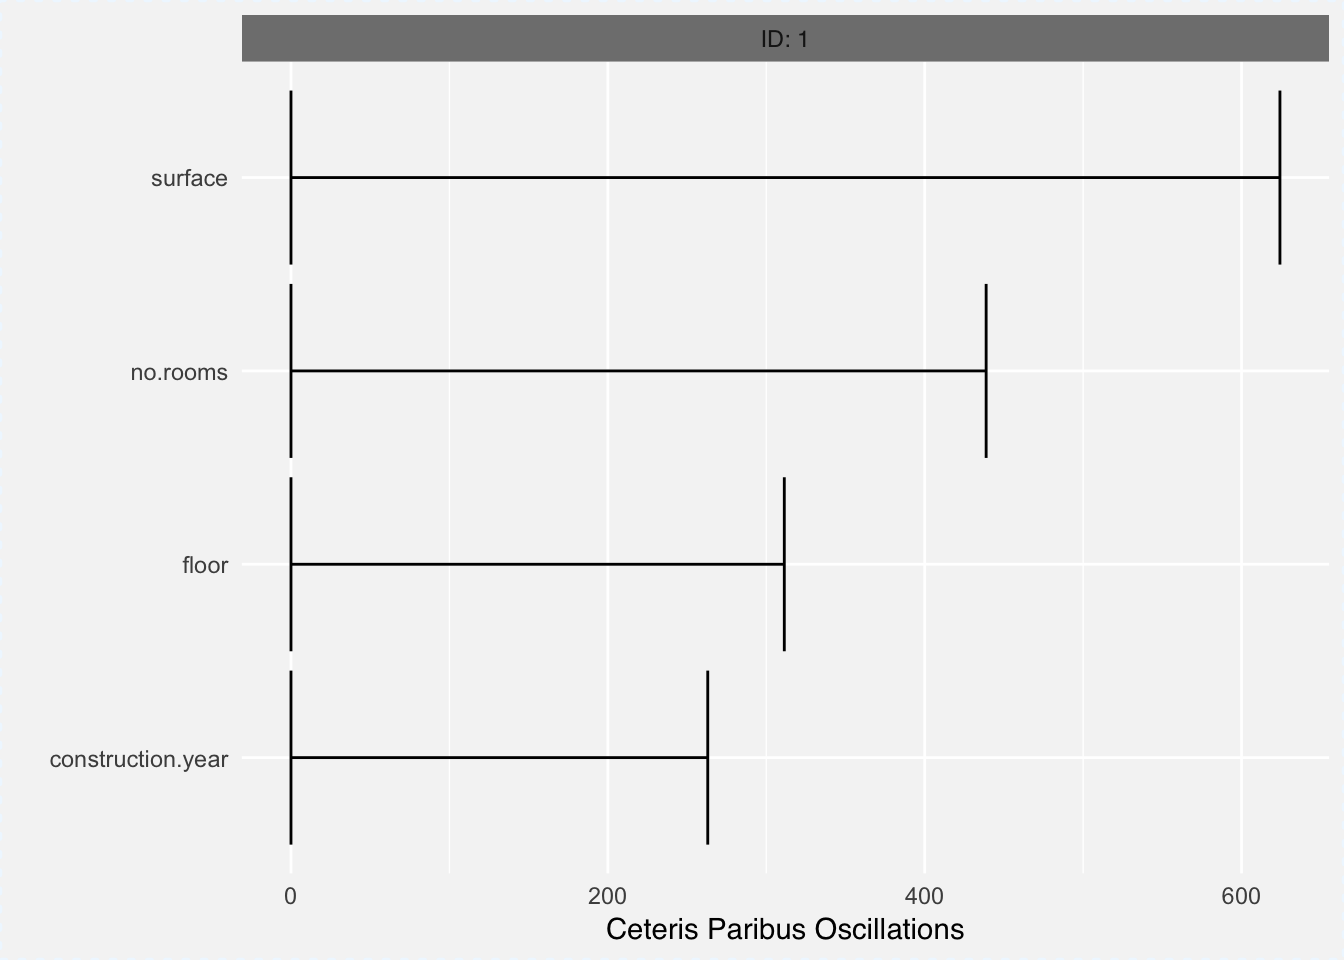
\includegraphics{PM_VEE_files/figure-latex/unnamed-chunk-36-1.pdf}

\hypertarget{advanced-usage-for-the-break_down-function}{%
\subsubsection{\texorpdfstring{Advanced usage for the
\texttt{break\_down}
function}{Advanced usage for the break\_down function}}\label{advanced-usage-for-the-break_down-function}}

The function \texttt{break\_down()} can take more arguments. The most
commonly used are:

\begin{itemize}
\tightlist
\item
  \texttt{x} a wrapper over a model created with function
  \texttt{DALEX::explain()},
\item
  \texttt{new\_observation} an observation to be explained is should be
  a data frame with structure that matches the training data,
\item
  \texttt{order} if specified then it can be a vector of characters
  (column names) or integers (column indexes) that specify order of
  variable conditioning. If not specified (default) then a one-step
  heuristic is used to determine the order,
\item
  \texttt{keep\_distributions} logical value.\\
  if \texttt{TRUE}, then additional diagnostic information is about
  conditional distributions is stored and can be plotted with the
  generic \texttt{plot()} function.
\end{itemize}

Let's see these additional arguments in action.

First we will specify order. You can use integer indexes or variable
names. Note that the second option is in most cases better because of
higher readability. Additionally, to reduce clutter in the plot we set
\texttt{max\_features\ =\ 3} argument in the \texttt{plot()} function.

\begin{Shaded}
\begin{Highlighting}[]
\KeywordTok{library}\NormalTok{(}\StringTok{"iBreakDown"}\NormalTok{)}
\NormalTok{bd_rf_order <-}\StringTok{ }\KeywordTok{break_down}\NormalTok{(explain_rf_v6,}
\NormalTok{                 johny_d,}
                 \DataTypeTok{order =} \KeywordTok{c}\NormalTok{(}\StringTok{"class"}\NormalTok{, }\StringTok{"age"}\NormalTok{, }\StringTok{"gender"}\NormalTok{, }\StringTok{"fare"}\NormalTok{, }\StringTok{"parch"}\NormalTok{, }\StringTok{"sibsp"}\NormalTok{, }\StringTok{"embarked"}\NormalTok{))}
\KeywordTok{plot}\NormalTok{(bd_rf_order, }\DataTypeTok{max_features =} \DecValTok{3}\NormalTok{) }
\end{Highlighting}
\end{Shaded}

\includegraphics{PM_VEE_files/figure-latex/unnamed-chunk-37-1.pdf}

The \texttt{plot\_distributions\ =\ TRUE} argument of
\texttt{break\_down()} function enriches model response with additional
information about conditional distribution.

It can be presented after setting \texttt{plot\_distributions\ =\ TRUE}
in the \texttt{plot()} function. Conditional distributions are presented
as vioplots. Red dots stand for conditional average model response. Thin
black lines between vioplots correspond to predictions for individual
observations. With them we can trace how model predictions change after
consecutive conditioning.

\begin{Shaded}
\begin{Highlighting}[]
\NormalTok{bd_rf_distr <-}\StringTok{ }\KeywordTok{break_down}\NormalTok{(explain_rf_v6,}
\NormalTok{                 johny_d,}
                 \DataTypeTok{order =} \KeywordTok{c}\NormalTok{(}\StringTok{"class"}\NormalTok{, }\StringTok{"age"}\NormalTok{, }\StringTok{"gender"}\NormalTok{, }\StringTok{"fare"}\NormalTok{, }\StringTok{"parch"}\NormalTok{, }\StringTok{"sibsp"}\NormalTok{, }\StringTok{"embarked"}\NormalTok{),}
                 \DataTypeTok{keep_distributions =} \OtherTok{TRUE}\NormalTok{)}
\KeywordTok{plot}\NormalTok{(bd_rf_distr, }\DataTypeTok{plot_distributions =} \OtherTok{TRUE}\NormalTok{) }
\end{Highlighting}
\end{Shaded}

\includegraphics{PM_VEE_files/figure-latex/unnamed-chunk-38-1.pdf}

\hypertarget{iBreakDown}{%
\section{iBreakDown for Variable Attributions with
Interactions}\label{iBreakDown}}

In the Section \ref{breakDown} we presented a model agnostic approach to
additive decomposition of model predictions. We also showed that for
non-additive moedls the proposed attribution depends on the ordering of
variables.

Lack of additivness means, that effect of one variable is modulated by
another variable(s). In such pair (or larger tuple) a single variable
does not contribute independently, therefore in model explanations they
should be presented together.

In this section we present an algorithm that identifies interactions
between pairs of variables and include such interactions in variable
decomposition plots. Here we present an algorithm for pairs of
variables, but it can be easily generalized to larger number of
variables.

\hypertarget{intuition-1}{%
\subsection{Intuition}\label{intuition-1}}

First, let's see an example of an interaction between two variables. We
will use real data from the Titanic dataset. Table
\ref{tab:titanicMaleSurvival} shows survival statistics for men on
Titanic. For the sake of simplicity, in this example we consider only
two variables - \texttt{age} and \texttt{class}. In the data
\texttt{age} is a continuous variable, but again, for simplicity we have
dychotomized it into two levels: boys (0-16 years old) and adults (17+
years old).

Suppose that we would like to explain factors that contribute to the
survival of kids from the second class. As we can read, the survival for
young passengers from 2nd class is 91.7\% (survived 11 out of 12 male
passengers in this group). It is higher than survival for men on titanic
which is 20.5\% (survived 352 out of 1716 men). So the question is, how
age and class contribute to this higher survival?

Let us consider two explanations, that correspond to two different
orderings:

\begin{itemize}
\tightlist
\item
  Overall men survival is 20.5\%, but when we condition on male
  passengers from 2nd class the survival is even lower, i.e.~13.5\%.
  Thus effect of the 2nd class is negative, it decreases the probability
  of survival by 7 percent points. Being a kid in the 2nd class is very
  lucky though. It changes of survival increase from 13.5\% (male 2nd
  class) to 91.7\% (boys from 2nd class). It's an increase by 78.2
  percent points. So the contributions are -7\% for class and +78.2\%
  for age.
\item
  Overall men survival is 20.5\%, but when we condition on young man
  then the survival is higher, i.e.~40.7\%. Thus the effect of age is
  positive, being a boy increases the probability of survival by 20.2
  percent points. Being a kid in 2nd class is even better, it changes
  the survival increase from 40.7\% (boys) to 91.7\% (boys from 2nd
  class). It's an increase by 51 percent points. So the contributions
  are +51\% for class and +20.2\% for age.
\end{itemize}

As we see these two paths leads to two very different explanations. They
differ not only in the size but also in the sign of attributed
importance. It has happend because one variable modulate effect on the
second variable as the moedl is not additive. Below we will show how to
deal with such cases.

\begin{longtable}[]{@{}llll@{}}
\caption{\label{tab:titanicMaleSurvival} Survival rates for men on Titanic.
Ratios show how many survived in each Class/Age
category.}\tabularnewline
\toprule
Class / Age & Kids (0-16) & Adults (\textgreater{}16) &
Total\tabularnewline
\midrule
\endfirsthead
\toprule
Class / Age & Kids (0-16) & Adults (\textgreater{}16) &
Total\tabularnewline
\midrule
\endhead
1st & 5/5 = 100\% & 57/175 = 32.6\% & 62/180 = 34.4\%\tabularnewline
2nd & 11/12 = 91.7\% & 13/166 = 7.8\% & 24/178 = 13.5\%\tabularnewline
3rd & 17/61 = 27.9\% & 58/430 = 13.5\% & 75/491 = 15.3\%\tabularnewline
deck crew & & 43/66 = 65.2\% & 43/66 = 65.2\%\tabularnewline
engineering crew & & 71/324 = 21.9\% & 71/324 = 21.9\%\tabularnewline
restaurant staff & & 1/67 = 1.5\% & 1/67 = 1.5\%\tabularnewline
victualling crew & 0/3 = 0\% & 76/407 = 18.7\% & 76/410 =
18.5\%\tabularnewline
Total & 33/81 = 40.7\% & 319/1635 = 19.5\% & 352/1716 =
20.5\%\tabularnewline
\bottomrule
\end{longtable}

The key intuition behind an iBreakDown algorithm is to include variable
interactions to the visual explanations. To do this we need to identify
some candidated for interactions. Here we propose a very simple
algorithm that will do this in two steps.

\begin{enumerate}
\def\labelenumi{\arabic{enumi}.}
\tightlist
\item
  First it will calculate variable contributions for each variable
  independently.
\item
  Second it will calculate joint effect for each pair of variables. If
  this effect is different than the sum of separate variables then such
  pair is identified as candidate for an interaction.
\end{enumerate}

\hypertarget{method-1}{%
\subsection{Method}\label{method-1}}

Identification of interactions in the model is performed in three steps
\citep{iBreakDownRPackage}

\begin{itemize}
\tightlist
\item
  Calculate a \emph{single-step} contribution for each variable.
\item
  Calculate a \emph{single-step} contribution for every pair of
  variables. Subtract individual contributions to assess the size of non
  additivness.
\item
  Order interaction effects and additive effects in a list to determin
  the final order for conditioning/explanations.
\end{itemize}

This simple intuition may be generalized into higher order interactions.

\hypertarget{single-step-contributions}{%
\subsubsection{Single step
contributions}\label{single-step-contributions}}

For a feature \(x_i\) we may define a single-step contribution as \[
\Delta^j =  \mathbb{E}[f(x)|x^j = x_*^j] - \mathbb{E}[f(x)].
\]

The expected model prediction \(\mathbb{E}[f(x)]\) is sometimes called
baseline or intercept and may be denoted as \(\Delta_\varnothing\).

Expected value \(\mathbb{E}[f(x)|x^j = x_*^j]\) corresponds to an
average prediction of a model \(f\) if feature \(x_j\) is fixed on
\(x^j_*\) coordinate from the observation to explain \(x_*\).

I.e. the \(\Delta^j\) is the difference between expected model response
after conditioning on \(j\) variable minus the expected model response.
\(\Delta^j\) measures a naive single-step local variable importance, it
indicates how much the average prediction of model \(f\) changes if
feature \(x^j\) is set on \(x_*^j\).

\hypertarget{two-steps-contributions}{%
\subsubsection{Two steps contributions}\label{two-steps-contributions}}

For a pair of variables \(x_i\), \(x_j\) we introduce a single-step
contribution as \[
\Delta^{ij} =  \mathbb{E}[f(x)|x^i = x_*^i, x^j = x_*^j] - \mathbb{E}[f(x)].
\]

And non additive component of this contribution as

\[
\Delta_{I}^{ij} =  \mathbb{E}[f(x)|x^i = x_*^i, x^j = x_*^j] -  \mathbb{E}[f(x)|x^i = x_*^i] -  \mathbb{E}[f(x)|x^j = x_*^j] + \mathbb{E}[f(x)].
\]

Or equivalently

\[
\Delta_{I}^{ij} = \Delta^{ij} - \Delta^i - \Delta^j. 
\]

\hypertarget{sequential-contributions}{%
\subsubsection{Sequential
contributions}\label{sequential-contributions}}

The \(\Delta_{I}^{ij}\) is the difference between collective effect of
variables \(x^i\) and \(x^j\) denoted as \(\Delta^{ij}\) and their
additive effects \(\Delta^{i}\) and \(\Delta^{j}\). Therefore,
\(\Delta_{I}^{ij}\) measures the importance of local lack-of-additivnes
(aka. interaction) between features \(i\) and \(j\). For additive models
\(\Delta_{I}^{ij}\) should be small\textasciitilde{}for any \(i\),
\(j\).

Note that contributions \(\Delta^{i}\) do not sum to final model
prediction. We only use them to determine the order of features in which
the instance shall be explained. To calculate contributions that have
the property of \emph{local accuracy} we need to introduce one more
symbol, that corresponds to the added contribution of feature \(i\) to
the set of features\textasciitilde{}\(J\).

\[
\Delta^{i|J} = \mathbf{E}[f(X)| x^{J\cup\{i\}} = x^{J\cup\{i\}}_{*}] -  \mathbf{E}[f(X)| x^{J} = x^{J}_{*}] =     \Delta^{J\cup\{i\}} - \Delta^{J}.
\]

And for pairs of features

\[
\Delta^{ij|J} = \mathbf{E}[f(X)| x^{J\cup\{i,j\}} = x^{J\cup\{i,j\}}_{*}] -  \mathbf{E}[f(X)| x^{J} = x^{J}_{*}] = 
    \Delta^{J\cup\{i,j\}} - \Delta^{J}.
\]

Once the order of single-step importance is determined based on
\(\Delta^i\) and \(\Delta_{I}^{ij}\) scores, the final explanation is
the attribution to the sequence of \(\Delta^{i|J}\) scores. These
contributions sum up to the model predictions, because

\[
\Delta^{1,2...p} = f(x_*) - E[f(X)].
\]

This approach can be generalized to interactions between any number of
variables.

The complexity of the calculation of single step attributions is
\(O(p)\) where \(p\) stands for the number of variables, wile complexity
for all pairs is \(O(p^2)\). The complexity of the consecutive
conditioning is \(O(p)\), thus the complexity of whole algorithm is
\(O(p^2)\).

\hypertarget{example-titanic-1}{%
\subsection{Example: Titanic}\label{example-titanic-1}}

In this example we will use a random forest model for Titanic data and
Johny D example - an 8 years old boy from 1st class.

In Table \ref{tab:titanicIBreakDownList} we showed expected model
responses \(\mathbb{E}[f(x)|x^i = x_*^i, x^j = x_*^j]\), single-step
effects \(\Delta^{ij}\) and non-additive effects \(\Delta_{I}^{ij}\) for
each variable and each pair of variables. All these values are
calculated locally for Johny D. These values are sorted along local
importance, most important to the top.

Based on this ordering a following sequence of variables are indentified
as informative: \texttt{age}, \texttt{fare:class}, \texttt{gender}.
\texttt{embarked}, \texttt{sibsp} and \texttt{parch}.

Once the ordering is specified, in the table
\ref{tab:titanicIBreakDownList2} we showed how the sequential
attribution is calculated. These values are then presented in the
iBreakDown plot \ref{fig:iBreakDownTitanicExamplePlot}.

\begin{longtable}[]{@{}lrrr@{}}
\caption{\label{tab:titanicIBreakDownList} For each variable and each pair
of variables we calculated the expected conditional model response, the
difference between conditional model response and the baseline and for
pairs of variables the non-additive contribution. Rows are sorted
according to the absolute value of the last column (if
provided).}\tabularnewline
\toprule
Variable & \(E[f(x):x^{ij}= x_*^{ij}]\) & \(\Delta^{ij}\) &
\(\Delta_I^{ij}\)\tabularnewline
\midrule
\endfirsthead
\toprule
Variable & \(E[f(x):x^{ij}= x_*^{ij}]\) & \(\Delta^{ij}\) &
\(\Delta_I^{ij}\)\tabularnewline
\midrule
\endhead
age & 0.505 & 0.270 &\tabularnewline
fare:class & 0.333 & 0.098 & -0.231\tabularnewline
class & 0.420 & 0.185 &\tabularnewline
fare:age & 0.484 & 0.249 & -0.164\tabularnewline
fare & 0.379 & 0.143 &\tabularnewline
gender & 0.110 & -0.125 &\tabularnewline
age:class & 0.591 & 0.355 & -0.100\tabularnewline
age:gender & 0.451 & 0.215 & 0.070\tabularnewline
fare:gender & 0.280 & 0.045 & 0.027\tabularnewline
embarked & 0.225 & -0.011 &\tabularnewline
embarked:age & 0.504 & 0.269 & 0.010\tabularnewline
parch:gender & 0.100 & -0.136 & -0.008\tabularnewline
sibsp & 0.243 & 0.008 &\tabularnewline
sibsp:age & 0.520 & 0.284 & 0.007\tabularnewline
sibsp:class & 0.422 & 0.187 & -0.006\tabularnewline
embarked:fare & 0.374 & 0.138 & 0.006\tabularnewline
sibsp:gender & 0.113 & -0.123 & -0.005\tabularnewline
fare:parch & 0.380 & 0.145 & 0.005\tabularnewline
parch:sibsp & 0.236 & 0.001 & -0.004\tabularnewline
parch & 0.232 & -0.003 &\tabularnewline
parch:age & 0.500 & 0.264 & -0.002\tabularnewline
embarked:gender & 0.101 & -0.134 & 0.002\tabularnewline
embarked:parch & 0.223 & -0.012 & 0.001\tabularnewline
fare:sibsp & 0.387 & 0.152 & 0.001\tabularnewline
embarked:class & 0.409 & 0.173 & -0.001\tabularnewline
gender:class & 0.296 & 0.061 & 0.001\tabularnewline
embarked:sibsp & 0.233 & -0.002 & 0.001\tabularnewline
parch:class & 0.418 & 0.183 & 0.000\tabularnewline
\bottomrule
\end{longtable}

\begin{longtable}[]{@{}lrr@{}}
\caption{\label{tab:titanicIBreakDownList2} Based on identified order we
calculated the expected conditional model response and the difference
between conditional model response with and without a specified
variable. These values are plotted in the iBreakDown
plot.}\tabularnewline
\toprule
Variable & \(\Delta^{i:J}\) & \(\Delta^{J\cup\{i\}}\)\tabularnewline
\midrule
\endfirsthead
\toprule
Variable & \(\Delta^{i:J}\) & \(\Delta^{J\cup\{i\}}\)\tabularnewline
\midrule
\endhead
intercept & & 0.235\tabularnewline
age = 8 & 0.269 & 0.505\tabularnewline
fare:class = 72:1st & 0.039 & 0.544\tabularnewline
gender = male & -0.083 & 0.461\tabularnewline
embarked = Southampton & -0.002 & 0.458\tabularnewline
sibsp = 0 & -0.006 & 0.452\tabularnewline
parch = 0 & -0.030 & 0.422\tabularnewline
\bottomrule
\end{longtable}

\begin{figure}

{\centering \includegraphics[width=0.8\linewidth]{PM_VEE_files/figure-latex/iBreakDownTitanicExamplePlot-1} 

}

\caption{(fig:iBreakDownTitanicExamplePlot) Break Down Plots with interactions for Johny D. }\label{fig:iBreakDownTitanicExamplePlot}
\end{figure}

\hypertarget{pros-and-cons-1}{%
\subsection{Pros and cons}\label{pros-and-cons-1}}

Break Down for interactions shares many features of Break Down for
single variables. Below we summarize unique strengths and weaknesses of
this approach.

\textbf{Pros}

\begin{itemize}
\tightlist
\item
  If interactions are present in the model, then additive contributions
  may be misleading. In such case the identification of interactions
  leads to better explanations.
\item
  Complexity of Break Down Algorithm is quadratic, what is not that bad
  if number of features is small or moderate.
\end{itemize}

\textbf{Cons}

\begin{itemize}
\tightlist
\item
  For large number of variables, the consideration of all interactions
  is both time consuming and sensitive to noise as the number of pairs
  grow faster than number of variables.
\item
  Identification of interaction is not based on significance testing,
  it's purely based on absolute empirical effects, thus for small
  samples this procedure is prone to errors.
\end{itemize}

\hypertarget{code-snippets-for-r-1}{%
\subsection{Code snippets for R}\label{code-snippets-for-r-1}}

In this section we present key features of the \texttt{iBreakDown}
package for R \citep{iBreakDownRPackage}. This package covers all
features presented in this chapter. It is available on CRAN and GitHub.
Find more examples at the website of this package
\texttt{https://modeloriented.github.io/iBreakDown/}.

All steps are very similar to these presented in the previouse chapter
for variable attributions. The only difference is that the
\texttt{break\_down()} function will now take
\texttt{interactions\ =\ TRUE} argument.

\textbf{Model preparation}

As in previous chapters we will use the random forest
\citep{R-randomForest} model \texttt{titanic\_rf\_v6} developed for the
Titanic dataset (see Section \ref{TitanicDataset}). Using the same model
will help us (1) to understand how the Break Down method works, (2) to
compare these explanations against methods presented in previous
chapters.

So let restore the \texttt{explain\_rf\_v6} explainer

\begin{Shaded}
\begin{Highlighting}[]
\KeywordTok{library}\NormalTok{(}\StringTok{"randomForest"}\NormalTok{)}
\NormalTok{explain_rf_v6 <-}\StringTok{ }\NormalTok{archivist}\OperatorTok{::}\KeywordTok{aread}\NormalTok{(}\StringTok{"pbiecek/models/9b971"}\NormalTok{)}

\KeywordTok{library}\NormalTok{(}\StringTok{"DALEX"}\NormalTok{)}
\NormalTok{johny_d <-}\StringTok{ }\NormalTok{archivist}\OperatorTok{::}\KeywordTok{aread}\NormalTok{(}\StringTok{"pbiecek/models/e3596"}\NormalTok{)}
\NormalTok{johny_d}
\end{Highlighting}
\end{Shaded}

\begin{verbatim}
##   class gender age sibsp parch fare    embarked
## 1   1st   male   8     0     0   72 Southampton
\end{verbatim}

The \texttt{iBreakDown::break\_down()} function calculates Break Down
contributions for a selected model around a selected observation.

The result from \texttt{break\_down()} function is a data frame with
additive attributions for selected observation.

The simplest use case is to set only the arguments - model explainers
and observation of interest.

By default only additive attributions are calculated. Use
\texttt{interactions\ =\ TRUE} argument to look for interactions.

\begin{Shaded}
\begin{Highlighting}[]
\KeywordTok{library}\NormalTok{(}\StringTok{"iBreakDown"}\NormalTok{)}
\NormalTok{bd_rf <-}\StringTok{ }\KeywordTok{break_down}\NormalTok{(explain_rf_v6,}
\NormalTok{                 johny_d,}
                 \DataTypeTok{interactions =} \OtherTok{TRUE}\NormalTok{)}

\NormalTok{bd_rf}
\end{Highlighting}
\end{Shaded}

\begin{verbatim}
##                                          contribution
## Random Forest v6: intercept                     0.235
## Random Forest v6: age = 8                       0.270
## Random Forest v6: fare:class = 72:1st           0.039
## Random Forest v6: gender = male                -0.083
## Random Forest v6: embarked = Southampton       -0.003
## Random Forest v6: sibsp = 0                    -0.006
## Random Forest v6: parch = 0                    -0.030
## Random Forest v6: prediction                    0.422
\end{verbatim}

The generic \texttt{plot()} function creates a Break Down plots.

\begin{Shaded}
\begin{Highlighting}[]
\KeywordTok{plot}\NormalTok{(bd_rf) }
\end{Highlighting}
\end{Shaded}

\includegraphics{PM_VEE_files/figure-latex/unnamed-chunk-43-1.pdf}

\hypertarget{shapley}{%
\section{SHapley Additive exPlanations (SHAP) and Average Variable
Attributions}\label{shapley}}

In the Section \ref{breakDown} we show a procedure that attributes parts
of model prediction to input features. We also show that in the presence
of interactions attributions depend on the feature ordering. One
solution to this problem is to find an ordering that put most important
features to the front. Other solution is introduced in the Section
\ref{iBreakDown} - identify interactions and show interactions in model
explanations.

In this section we introduce another, very popular approach that deal
with feature ordering. Basically, the problem of ordering is solved by
averaging over all possible orderings. Or at least some large number of
sampled orderings. Additionally, such average is closely linked with
Shapley values developed originally for cooperative games.

This approach was first introduced in \citep{imeJLMR} and
\citep{Strumbelj2014}. Wide adoption of this method comes with a NIPS
2017 paper \citep{SHAP} and python library SHAP \citep{shapPackage}.
Authors of the SHAP (SHapley Additive exPlanations) method introduced an
efficient algorithm for tree-based models \citep{TreeSHAP} and show that
Shapley values is an unification of a collection of different commonly
used techniques for model explanations.

\hypertarget{intuition-2}{%
\subsection{Intuition}\label{intuition-2}}

Figure \ref{fig:shap10orderings} shows Break Down attributions for 10
random orderings for Titanic dataset. As we see there are differences in
feature attribution. The most striking ones are linked with features
\texttt{fare} or \texttt{class}. They attribution may be positive or
negative depending on the ordering

\begin{figure}

{\centering \includegraphics[width=1\linewidth]{figure/shap_10_replicates} 

}

\caption{(fig:shap10orderings) Break Down plots for 10 random orderings. Each panel shows a single ordering}\label{fig:shap10orderings}
\end{figure}

SHAP attributions are averages across all (or at least large number) of
different orderings. See for example Figure \ref{fig:shapOrdering}. In a
single plot we summarize all orderings from Figure
\ref{fig:shap10orderings}. Violet boxplots show distributions for
attributions for a selected variable, while length of the bar stands for
an average attribution.

\begin{figure}

{\centering \includegraphics[width=0.7\linewidth]{figure/shap_ordering} 

}

\caption{(fig:shapOrdering) Summary for 10 random orderings. Boxplots show distribution of feature attributions. Bars stand for average attributions.}\label{fig:shapOrdering}
\end{figure}

\hypertarget{method-2}{%
\subsection{Method}\label{method-2}}

SHapley Additive exPlanations are based on \emph{Shapley Values}, a
solution concept in cooperative game theory developed by Lloyd Shapley.

Consider a following problem. A coalition of players cooperates, and
obtains a certain overall gain from that cooperation. Players are not
identical, different players may have different importance. Cooperation
is beneficial, from cooperation they got more than from individual
actions. The problem to solve is how to distribute the generated surplus
among the players? The Shapley value provides one possible fair answer
to this question \citep{shapleybook1952}.

Now let's translate this problem to machine learning settings. Instead
of players we have features and instead of coalitions we have specific
settings of values for features in the coalition. The payoff from a
coalition is the model response for a selected setting. Problem to
solve: how to distribute model response to particular features. Shapley
values are defined for a single instance \(x^*\). The idea of using
Shapley values for feature attribution was introduced in
\citep{imeJLMR}. Here we present a different notation more suited with
approach presented in previous sections.

Let \(v(S)\) stand for value of coalition of \(S\) features, defined as
\[
v(x^*, S) = E[f(X) | X_S = x^*_S].
\] The value is defined as expected model response given features in the
set \(S\) are set to values in the selected instance \(x^*\). Expected
value averages across all features that are not in the set \(S\).

A special case is for empty coalition. Its value is an expected model
response \[
v(x^*, \emptyset) = E[f(X)].
\]

Shapley values may be defined as \[
\varphi(i) = \frac{1}{p!} \sum_{\pi} [v(x^*, \pi(i) \cup \{i\}) - v(x^*, \pi(i))]  
\] where \(p\) is a number of all features, \(p!\) is number of all
possible orderings, \(\pi\) is an ordering and \(\pi(i)\) are all
features in the ordering \(\pi\) that appear before feature \(i\). Thus
the \(v(\pi(i) \cup \{i\}) - v(\pi(i))\) corresponds to a difference in
value of a coalition \(v(\pi(i))\) when feature \(i\) is added to it.

Of course for large \(p\) it is not feasible to consider all \(p!\)
permutations. A Monte Carlo estimator of this value was introduced in
\citep{Strumbelj2014} and efficient implementation of Shapley values was
introduced in \citep{SHAP}. Later in this chapter we will use a crude
estimator on \(\varphi(i)\) in which instead of all \(p!\) permutations
we average across \(B\) randomly selected permutations.

Alternative formulation of Shapley values averages across coalitions not
orderings.

\[
\varphi(i) = \frac 1{p}\sum_{S \subseteq \{1:p\}\setminus \{i\}}  {{p-1}\choose{|S|}}^{-1} \left[ v(x^*, S \cup \{i\}) - v (x^*, S) \right]
\]

Note that the number of all subsets is \(2^{p-1}\) is much smaller than
number of all orderings \(p!\). Binomial coefficients weight according
to number of ordering with selected prefix coalition.

\textbf{Properties}

Shapley values are proven to be fair. And here fairness means that they
are a single unique solution with following properties. Proved for
cooperative games and then translated to machine learning.

\begin{itemize}
\tightlist
\item
  Symmetry. If two features are interchangeable, i.e.~contribute equally
  to all coalitions
\end{itemize}

\[
\forall_{S} v(x^*, S \cup \{i\}) = v(x^*, S \cup \{j\})
\]

then they should have equal Shapley values

\[
\varphi(i) = \varphi(j).
\]

\begin{itemize}
\tightlist
\item
  Dummy feature. If a features does not contribute to any coalitions \[
  \forall_{S} v(x^*, S \cup \{i\}) = v(x^*, S)
  \]
\end{itemize}

then it should have Shapley value equal to 0

\[
\varphi(i) = 0.
\]

\begin{itemize}
\item
  Additivity. If a model \(f\) is sum of two other models \(g\) and
  \(h\) then Shapley value calculated for model \(f\) is a sum of
  Shapley values for \(g\) and \(h\).
\item
  Local accuracy. Sum of Shapley values is equal to the model response
\end{itemize}

\[
f(x^*) - v(x^*, \emptyset) = \sum_{i=1}^p   \varphi(i). 
\]

\hypertarget{example-titanic-2}{%
\subsection{Example: Titanic}\label{example-titanic-2}}

Let us again consider explanation for prediction of the
\texttt{titanic\_rf\_v6} model for \emph{Johny D}, an 8-years old boy
from 1st class.

In Figure \ref{fig:shappJohny02} we have presented distribution of
attributions for random 25 orderings. As we see, young age of Johny D
has positive effect in all orderings. An average age-effect is equal
\(0.2525\). Similarly, effect of being male is in all cases negative for
this model, on average the negative effect is \(-0.0908\).

Things get complicated for \texttt{fare} and \texttt{class} features.
Depending on the order one or another is largely positive or negative.
In the section \ref{iBreakDown} we showed them as a pair, which should
not be separated. Here we show average attributions for each feature.

\begin{figure}

{\centering \includegraphics[width=0.8\linewidth]{PM_VEE_files/figure-latex/shappJohny02-1} 

}

\caption{(fig:shappJohny02) Average attributions for Johny D. Violet boxplots show distributions of attributions.}\label{fig:shappJohny02}
\end{figure}

Note, that in most applications the detailed information about
distribution of orderings will be unnecessary complicated. So it is more
common to keep only information about Shapley values as it is presented
in Figure \ref{fig:shappJohny01}.

\begin{figure}

{\centering \includegraphics[width=0.8\linewidth]{PM_VEE_files/figure-latex/shappJohny01-1} 

}

\caption{(fig:shappJohny01) Average attributions for Johny D. }\label{fig:shappJohny01}
\end{figure}

Table \ref{tab:shapOrderingTable} shows average attributions for Johny
D.

\begin{longtable}[]{@{}lr@{}}
\caption{\label{tab:shapOrderingTable} Average attributions for Johny
D.}\tabularnewline
\toprule
feature & avg. attribution\tabularnewline
\midrule
\endfirsthead
\toprule
feature & avg. attribution\tabularnewline
\midrule
\endhead
age = 8 & 0.2525\tabularnewline
class = 1st & 0.0246\tabularnewline
embarked = Southampton & -0.0032\tabularnewline
fare = 72 & 0.0140\tabularnewline
gender = male & -0.0943\tabularnewline
parch = 0 & -0.0097\tabularnewline
sibsp = 0 & 0.0027\tabularnewline
\bottomrule
\end{longtable}

\hypertarget{pros-and-cons-2}{%
\subsection{Pros and cons}\label{pros-and-cons-2}}

Shapley Values give a uniform approach to decompose model prediction
into parts that can be attributed additively to variables. Below we
summarize key strengths and weaknesses of this approach.

\textbf{Pros}

\begin{itemize}
\tightlist
\item
  There is a nice theory based on cooperative games.
\item
  \citep{SHAP} shows that this method unifies different approaches to
  additive features attribution, like DeepLIFT, Layer-Wise Relevance
  Propagation, LIME.
\item
  There is an efficient implementation available for Python and ports or
  reimplementations for R.
\item
  \citep{SHAP} shows more desired properties of this method, like
  symmetry or Local accuracy.
\end{itemize}

\textbf{Cons}

\begin{itemize}
\tightlist
\item
  The exact calculation of Shapley values is time consuming.
\item
  If the model is not additive, then the Shapley scores may be
  misleading. And there is no way to determine if model is far from
  additiveness.
\item
  In the cooperation games the goal was to distribute payoff among
  payers, but in machine learning we want to understand how players
  affect payoff. Thus we are not limited to independent payoffs for
  players.
\end{itemize}

Note that for an additive model other approaches like these presented in
Sections \ref{breakDown}, \ref{iBreakDown} and \ref{shapley} lead to
same variable contributions.

\hypertarget{code-snippets-for-r-2}{%
\subsection{Code snippets for R}\label{code-snippets-for-r-2}}

In this section we present key features of the R package
\texttt{iBreakDown} \citep{iBreakDownRPackage} which is a part of
\texttt{DrWhy.AI} universe and covers methods presented in this chapter.
More details and examples can be found at
\texttt{https://modeloriented.github.io/iBreakDown/}.

Note that there are also other R packages that offer similar
functionality, like \texttt{shapper} \citep{shapperPackage} which is a
wrapper over SHAP python library \citep{shapPackage} and \texttt{iml}
\citep{imlRPackage}.

In this section, we use the random forest \citep{R-randomForest} model
\texttt{titanic\_rf\_v6} developed for the Titanic dataset (see Chapter
\ref{TitanicDataset}).

So let restore the \texttt{titanic\_rf\_v6} model and explainer created
with the \texttt{explain()} function from \texttt{DALEX} package
\citep{R-DALEX}.

\begin{Shaded}
\begin{Highlighting}[]
\KeywordTok{library}\NormalTok{(}\StringTok{"randomForest"}\NormalTok{)}
\NormalTok{explain_rf_v6 <-}\StringTok{ }\NormalTok{archivist}\OperatorTok{::}\KeywordTok{aread}\NormalTok{(}\StringTok{"pbiecek/models/9b971"}\NormalTok{)}

\KeywordTok{library}\NormalTok{(}\StringTok{"DALEX"}\NormalTok{)}
\NormalTok{johny_d <-}\StringTok{ }\NormalTok{archivist}\OperatorTok{::}\KeywordTok{aread}\NormalTok{(}\StringTok{"pbiecek/models/e3596"}\NormalTok{)}
\NormalTok{johny_d}
\end{Highlighting}
\end{Shaded}

Here again we will use a data frame \texttt{johny\_d} with a single row,
that describes an 8-years old boy that travels in the first class
without parents and siblings. Then, we obtain the model prediction for
this instance with the help of the `predict()' function.

\begin{Shaded}
\begin{Highlighting}[]
\KeywordTok{predict}\NormalTok{(explain_rf_v6, johny_d)}
\end{Highlighting}
\end{Shaded}

\begin{verbatim}
## [1] 0.422
\end{verbatim}

First, we will recreate Figure \ref{fig:shappJohny01}. To do this we use
function \texttt{iBreakDown::shap()} that calculates \texttt{B} random
orderings and average Shapley contributions. This function takes an
explainer created with \texttt{DALEX::explain()} function and an
observation for which attributions shall be calculated. Additionally one
can specify \texttt{B} number of orderings to sample.

The generic function \texttt{plot()} shows Shapley values with
corresponding boxplots.

\begin{Shaded}
\begin{Highlighting}[]
\KeywordTok{library}\NormalTok{(}\StringTok{"iBreakDown"}\NormalTok{)}

\NormalTok{shap_johny <-}\StringTok{ }\KeywordTok{shap}\NormalTok{(explain_rf_v6, johny_d, }\DataTypeTok{B =} \DecValTok{25}\NormalTok{)}
\KeywordTok{plot}\NormalTok{(shap_johny) }
\end{Highlighting}
\end{Shaded}

\includegraphics{PM_VEE_files/figure-latex/unnamed-chunk-49-1.pdf}

Figure \ref{fig:shappJohny02} is generated in the same way. The only
difference is that boxplots are not plotted. Use the
\texttt{show\_boxplots} argument to decide whatever they shall be added
or not.

\begin{Shaded}
\begin{Highlighting}[]
\KeywordTok{plot}\NormalTok{(shap_johny, }\DataTypeTok{show_boxplots =} \OtherTok{FALSE}\NormalTok{) }
\end{Highlighting}
\end{Shaded}

\includegraphics{PM_VEE_files/figure-latex/unnamed-chunk-50-1.pdf}

Function \texttt{shap()} results a data frame with attributions for
every ordering. Having all these values we can calculated not only
Shapley values (averages) but also some other statistics, like quintiles
or range for feature attributions.

\begin{Shaded}
\begin{Highlighting}[]
\NormalTok{shap_johny}
\end{Highlighting}
\end{Shaded}

\begin{verbatim}
##                                   min            q1       median
## Random Forest v6-age       0.10631717  0.1710566380  0.252221985
## Random Forest v6-class    -0.05615224 -0.0008022202  0.060401903
## Random Forest v6-embarked -0.01580879 -0.0105541459 -0.007472134
## Random Forest v6-fare     -0.08729950 -0.0713928410 -0.045135931
## Random Forest v6-gender   -0.17778251 -0.1248278206 -0.105988219
## Random Forest v6-parch    -0.03033983 -0.0134748527 -0.009966017
## Random Forest v6-sibsp    -0.01059538 -0.0059755324 -0.001904848
##                                    mean           q3          max
## Random Forest v6-age       0.2370556593  0.269811509  0.357347531
## Random Forest v6-class     0.0703436701  0.179579067  0.185606706
## Random Forest v6-embarked -0.0063245310 -0.004847558  0.007968283
## Random Forest v6-fare     -0.0014576167 -0.003210340  0.195174445
## Random Forest v6-gender   -0.1004931944 -0.078935433 -0.042726778
## Random Forest v6-parch    -0.0116046398 -0.003649751 -0.001842320
## Random Forest v6-sibsp    -0.0008288174  0.003267784  0.014658813
\end{verbatim}

\begin{Shaded}
\begin{Highlighting}[]
\KeywordTok{library}\NormalTok{(}\StringTok{"dplyr"}\NormalTok{)}
\NormalTok{shap_johny }\OperatorTok
\StringTok{  }\KeywordTok{group_by}\NormalTok{(variable) }\OperatorTok
\StringTok{  }\KeywordTok{summarise}\NormalTok{(}\DataTypeTok{avg =} \KeywordTok{mean}\NormalTok{(contribution),}
            \DataTypeTok{q10 =} \KeywordTok{quantile}\NormalTok{(contribution, }\FloatTok{0.1}\NormalTok{),}
            \DataTypeTok{q90 =} \KeywordTok{quantile}\NormalTok{(contribution, }\FloatTok{0.9}\NormalTok{)) }\OperatorTok
\StringTok{  }\KeywordTok{arrange}\NormalTok{(}\OperatorTok{-}\KeywordTok{abs}\NormalTok{(avg))}
\end{Highlighting}
\end{Shaded}

\begin{verbatim}
## # A tibble: 7 x 4
##   variable       avg      q10      q90
##   <fct>        <dbl>    <dbl>    <dbl>
## 1 age       0.237     0.158    0.313  
## 2 gender   -0.100    -0.133   -0.0555 
## 3 class     0.0703   -0.0293   0.185  
## 4 parch    -0.0116   -0.0303  -0.00304
## 5 embarked -0.00632  -0.0124   0.00348
## 6 fare     -0.00146  -0.0714   0.146  
## 7 sibsp    -0.000829 -0.00835  0.00824
\end{verbatim}

\hypertarget{LIME}{%
\section{Local Interpretable Model-Agnostic Explanations
(LIME)}\label{LIME}}

\hypertarget{introduction-1}{%
\subsection{Introduction}\label{introduction-1}}

Ceteris Paribus profiles introduced in the Chapter \ref{ceterisParibus}
work best for models with small number of interpretable features. In
this case it makes sense to explore feature by feature and analyze how a
single feature affects model predictions

Break Down and Shapley attributions introduced in the Chapter
\ref{breakDown} work best for small and moderate number of features.
These attributions are not as detailed as Ceteris Paribus profiles, but
can handle more variables that are presented by narrow bars.

Both these approaches are not well suited for high-dimensional data. For
instance in bioinformatics when working with gene expression, mutations
or methylation it is not uncommon to have thousands or even million of
features. If most of them are binary low/high, present/absent,
wild/mutated then Ceteris Paribus and Break Down plots become
unreadable. In such cases an useful alternatives are sparse explainers.
The most popular example of such explainers is LIME and its
modifications.

The LIME method was originally proposed in the paper \emph{Why Should I
Trust You?: Explaining the Predictions of Any Classifier} \citep{lime}.
The acronym stands for Local Interpretable Model-Agnostic Explanations.
The key idea behind this method is to locally approximate a black-box
model by a sparse local glass-box surrogate model, which is easier to
interpret.

\hypertarget{intuition-3}{%
\subsection{Intuition}\label{intuition-3}}

The intuition behind LIME is presented in Figure \ref{fig:limeEx}. We
want to understand a complex black-box model around a single instance.
Here the black box model is a binary classifier and colored areas in the
plot correspond to its decision regions. We are interested in instance
explanation, and the instance of interest is marked with large black
dot. Having some artificial dataset around this black dot we can train a
glass-box model that will locally approximate the black-box model. The
glass-box model may then serves as local explainer for the complex
model.

We may select different classes of glass-box models, e.g.~linear models.
The important part is to keep it sparse and low-dimensions, this way the
surrogate model is easier to explain. The most typical choices for
glass-box models are regularized linear models like LASSO regression or
decision trees.

\begin{figure}

{\centering \includegraphics[width=0.7\linewidth]{figure/limeEx} 

}

\caption{(fig:limeEx) A schematic idea behind local model approximations. Colors stand for decision regions for black-box model. We want to explain model decision for the largest black point. To do this we create artificial points around point of interest and train a glass-box model. Here it's a logistic regression presented as a dashed line.}\label{fig:limeEx}
\end{figure}

\hypertarget{method-3}{%
\subsection{Method}\label{method-3}}

The objective is to find a local model \(M_{*}\) that approximates a
black box model \(f\) around the point of interest \(x_*\). This
intuition can be formalized in a following formula

\[
M(x_{*}) = \arg \min_{g \in G} L(f, g, \Pi_{x_*}) + \Omega (g). 
\] For a selected instance \(x_*\) we are looking for a local model
\(g\) from the class \(G\) of interpretable models. The model shall be
simple so we add penalty for the model complexity measured as
\(\Omega(g)\). And the white-box model \(g\) shall approximate well the
black-box model \(f\) locally, where locality is defined by neighborhood
\(\Pi_{x_*}\) of \(x^*\). The \(L\) stands for some goodness of fit
measure like for example likelihood.

Note that functions \(f\) and \(g\) may work on different data
representations. The black-box
\(f(x):\mathcal X \rightarrow \mathcal R\) works on original feature
space \(\mathcal X\) while the glass-box function
\(g:\mathcal X' \rightarrow \mathcal R\) usually works on an
interpretable feature space \(\mathcal X'\), which is in many
applications smaller. We will present some examples for \(\mathcal X'\)
in the next section, but for now let's just assume that function \(h\)
transforms \(\mathcal X\) on \(\mathcal X'\).

Let's limit the class \(G\) of interpretable models to sparse linear
models. Following algorithm may be used to find an interpretable
surrogate model that selects \(K\) most important interpretable
features.

\begin{verbatim}
Input: N - length of sample for surrogate model
Input: K - length of explanation
1. Let x' = h(x) be an interpretable version of x
2. for i in 1...N {
3.   z'[i] <- sample_around(x')
4.   y'[i] <- f(z[i]) # prediction for a new observation
5.   w'[i] <- similarity(x, z[i])
6. }
7. return K-LASSO(y', x', w')
\end{verbatim}

Where \(K-LASSO(y', x', w')\) stands for weighted LASSO linear
regression that selects \(K\) most important features based on new
dataset \((y', x')\) weighted with \(w'\). This algorithm selects \(K\)
most important interpretable features.

As it is presented in the paper \citep{lime}, the LIME method has
following properties:

\begin{itemize}
\tightlist
\item
  \emph{model-agnostic}, they do not imply any assumptions on model
  structure, \(f\) can be any function,
\item
  \emph{interpretable representation}, model input is transformed into a
  feature space that is easier to understand. One of applications comes
  from image data, single pixels are not easy to interpret, thus the
  LIME method decompose image into a series of super pixels, that are
  easier to interpret to humans,
\item
  \emph{local fidelity} means that the explanations shall be locally
  well fitted to the black-box model.
\end{itemize}

Where it comes to the implementation of this idea there are at least
three important steps, which will be presented in consecutive
subsections.

\hypertarget{interpretable-data-representation}{%
\subsubsection{Interpretable data
representation}\label{interpretable-data-representation}}

It is important to remember that functions \(f\) and \(g\) may work on
different data representations.

For example, let's consider a VGG16 neural network trained for ImageNet
data. Such network takes an image of the size 244x244 pixels as an input
and predicts an image category out of 1000 classes. The original input
space is 3x244x244 = 178608 dimensional as single dimensional is a
single color channel for a single pixel. Explanations in such input
space would be hard to interpret. Instead, the input space is
transformed into superpixels - binary features that can be turned on or
off. Figure \ref{fig:duckHorse06} shows an example 100 superpixels
created for some ambiguous picture.

In this case the black box model \(f\) works on \(\mathcal X\) which is
\(\mathcal R^{178608}\) while \(g\) works on interpretable binary space
of 100 superpixels \(\mathcal X' = [0,1]^{100}\).

Superpixels are frequent choices for image data. For text data words are
frequently used as interpretable features. For tabular data sometimes
continuous features are discretized.

\begin{figure}

{\centering \includegraphics[width=1\linewidth]{figure/duck_horse_06} 

}

\caption{(fig:duckHorse06) The left panel shows an ambiguous picture, half horse and hals duck. The right panel shows 100 superpixes identified for this figure.}\label{fig:duckHorse06}
\end{figure}

\hypertarget{sampling-around-point-of-interest}{%
\subsubsection{Sampling around point of
interest}\label{sampling-around-point-of-interest}}

In order to fit surrogate local model \(g\) we need new data points
around point of interest. It is not enough to sample points from
original dataset, because in very highdimensional space the input
dataset is very sparse and points are ,,far'' from each other.

This is why the training data for surrogate model is created through
some perturbations of the point of interest.

For binary interpretable input space the common choice is to sample
subset of features (i.e.~new datapoints are the point of interest with
some random number of features switched to 0).

For nonbinary features various propositions are introduced in different
papers.

In our example with the duck-horse samples around the image are subsets
of superpixels.

\hypertarget{fitting-a-glass-box-model}{%
\subsubsection{Fitting a glass-box
model}\label{fitting-a-glass-box-model}}

Once the new data are sampled around the point of interest we are ready
to create an interpretable model \(g\) from class \(G\).

The most common choices for \(G\) are linear models (for regression) or
generalized linear models (for classification). In order to get sparse
models the LASSO or similar regularisation/feature selection is used. An
alternative choice is classification and regression trees.

In our example we are using \(K-LASSO\) method which selects \(K\) super
pixels that are the most influential when it comes to model prediction.
In the Figure \ref{fig:duckHorse04} we present explanations for the top
2 classes selected by the model VGG16. For each class the top \(K\)
superpixels / interpretabble features are highlighted

Interesting to see that the superpixel that shows the nib is influential
when it comes to prediction \emph{`goose'} and superpixels linked with
white fur are linked with prediction \emph{`standard poodle'}.

\begin{figure}

{\centering \includegraphics[width=1\linewidth]{figure/duck_horse_04} 

}

\caption{(fig:duckHorse04) LIME explanations for two classess identified by the VGG16 network with ImageNet weights.}\label{fig:duckHorse04}
\end{figure}

\hypertarget{example-titanic-3}{%
\subsection{Example: Titanic}\label{example-titanic-3}}

Let us again consider explanation for prediction of the
\texttt{titanic\_rf\_v6} model for \emph{Johny D}, an 8-years old boy
from 1st class.

In Figure \ref{fig:LIMEexample01} we have presented explanations
generated with the LIME method. Three variables were identified as the
most influential, age, gender and class.

\begin{figure}

{\centering \includegraphics[width=0.6\linewidth]{figure/LIMEexample01} 

}

\caption{(fig:LIMEexample01) LIME explanations for single instance Johny D and generated for Random Forest v6 model.}\label{fig:LIMEexample01}
\end{figure}

It is important here to mention how interpretable features are created.
For tabular data the most common approach is to discretized continuous
variables and combine levels in categorical variables.

Figure \ref{fig:LIMEexample02} shows how interpretable feature can be
extracted from Ceteris Paribus Profile for the variable \texttt{age}.

\begin{figure}

{\centering \includegraphics[width=0.6\linewidth]{figure/LIMEexample02} 

}

\caption{(fig:LIMEexample02) Interpretable local feature generated for age variable. LIME explanations for single instance Johny D and generated for Random Forest v6 model }\label{fig:LIMEexample02}
\end{figure}

Different implementations of the LIME method have different algorithms
for extraction of interpretable features, different methods for sampling
and different methods for weighting.

In the section \emph{Code snippets for R} we present different available
implementations.

\hypertarget{pros-and-cons-3}{%
\subsection{Pros and cons}\label{pros-and-cons-3}}

Local approximations are model agnostic, can be applied to any
predictive model. Below we summarize key strengths and weaknesses of
this approach.

\textbf{Pros}

\begin{itemize}
\tightlist
\item
  This method is highly adopted in text analysis and image analysis, in
  part thanks to the interpretable data representations.
\item
  The intuition behind the method is straightforward, fit simple model
  to approximate a complex model.
\item
  Model explanations are sparse, thus only small number of features are
  in the surrogate models used what makes it easier to explain.
\item
  The LIME method can be applied to high dimensional models.
\end{itemize}

\textbf{Cons}

\begin{itemize}
\tightlist
\item
  For continuous variables and tabular data it is not that easy to find
  interpretable representations. IMHO this problem is not solved yet.
\item
  The black-box model approximated the data and the glass-box model
  approximates the black box model. We do not have control over the
  quality of local fit of the glass-box model, thus the surrogate model
  may be misleading.
\item
  Due to the \emph{curse of dimensionality}, for high dimensional space
  points are sparse. Measuring of being local is tricky.
\end{itemize}

\hypertarget{code-snippets-for-r-3}{%
\subsection{Code snippets for R}\label{code-snippets-for-r-3}}

The LIME methods and it's clones are now implemented in various R and
python packages, see for example \texttt{lime} \citep{R-lime} which is a
port of LIME python library \citep{shapPackage}, \texttt{live}
\citep{R-live} and \texttt{localModel} \citep{localModelPackage} and
\texttt{iml} \citep{imlRPackage}.

These packages are different in a way how they turn continuous variables
into interpretable features. For example, package \texttt{lime} performs
global discretization using quartiles, \texttt{localModel} performs
local discretization using Ceteris Paribus profiles, while \texttt{live}
and \texttt{iml} works directly on continuous variables. Also they
differ in terms of which surrogate models they use and how new instances
are being sampled. For these reasons these packages results different
explanations.

Below we present explanations returned for these four methods for the
Johny D and \texttt{titanic\_rf\_v6} model.

\begin{Shaded}
\begin{Highlighting}[]
\KeywordTok{library}\NormalTok{(}\StringTok{"DALEX"}\NormalTok{)}
\KeywordTok{library}\NormalTok{(}\StringTok{"randomForest"}\NormalTok{)}

\NormalTok{titanic <-}\StringTok{ }\NormalTok{archivist}\OperatorTok{::}\KeywordTok{aread}\NormalTok{(}\StringTok{"pbiecek/models/27e5c"}\NormalTok{)}
\NormalTok{titanic_rf_v6 <-}\StringTok{ }\NormalTok{archivist}\OperatorTok{::}\KeywordTok{aread}\NormalTok{(}\StringTok{"pbiecek/models/31570"}\NormalTok{)}
\NormalTok{johny_d <-}\StringTok{ }\NormalTok{archivist}\OperatorTok{::}\KeywordTok{aread}\NormalTok{(}\StringTok{"pbiecek/models/e3596"}\NormalTok{)}
\end{Highlighting}
\end{Shaded}

\hypertarget{the-lime-package}{%
\subsubsection{\texorpdfstring{\textbf{The lime
package}}{The lime package}}\label{the-lime-package}}

An example code snippet for the \texttt{lime} package is presented
below. Key parts are function \texttt{lime::lime} which creates an
explainer and \texttt{lime::explain} which evaluates explanations.

Resulting explanations are presented in Figure
\ref{fig:limeExplLIMETitanic}.

For continuous variables \texttt{lime} package discretizes features by
using quartiles. This is why in the explanation we have
\texttt{age\ \textless{}\ 22}.

\begin{Shaded}
\begin{Highlighting}[]
\KeywordTok{library}\NormalTok{(}\StringTok{"lime"}\NormalTok{)}
\NormalTok{model_type.randomForest <-}\StringTok{ }\ControlFlowTok{function}\NormalTok{(x, ...) }\StringTok{"classification"}
\NormalTok{lime_rf <-}\StringTok{ }\KeywordTok{lime}\NormalTok{(titanic[,}\KeywordTok{colnames}\NormalTok{(johny_d)], titanic_rf_v6)}
\NormalTok{lime_expl <-}\StringTok{ }\NormalTok{lime}\OperatorTok{::}\KeywordTok{explain}\NormalTok{(johny_d, lime_rf, }\DataTypeTok{labels =} \StringTok{"yes"}\NormalTok{, }\DataTypeTok{n_features =} \DecValTok{4}\NormalTok{, }\DataTypeTok{n_permutations =} \DecValTok{1000}\NormalTok{)}
\NormalTok{lime_expl}

\CommentTok{#      model_type case label label_prob  model_r2 model_intercept model_prediction}
\CommentTok{#1 classification    1    no      0.602 0.5806297       0.5365448        0.5805939}
\CommentTok{#2 classification    1    no      0.602 0.5806297       0.5365448        0.5805939}
\CommentTok{#3 classification    1    no      0.602 0.5806297       0.5365448        0.5805939}
\CommentTok{#4 classification    1    no      0.602 0.5806297       0.5365448        0.5805939}
\CommentTok{#  feature feature_value feature_weight  feature_desc                 data   prediction}
\CommentTok{#1    fare            72     0.00640936  21.00 < fare 1, 2, 8, 0, 0, 72, 4 0.602, 0.398}
\CommentTok{#2  gender             2     0.30481181 gender = male 1, 2, 8, 0, 0, 72, 4 0.602, 0.398}
\CommentTok{#3   class             1    -0.16690730   class = 1st 1, 2, 8, 0, 0, 72, 4 0.602, 0.398}
\CommentTok{#4     age             8    -0.10026475     age <= 22 1, 2, 8, 0, 0, 72, 4 0.602, 0.398}

\KeywordTok{plot_features}\NormalTok{(lime_expl)}
\end{Highlighting}
\end{Shaded}

\begin{figure}

{\centering \includegraphics[width=0.6\linewidth]{figure/lime_expl_lime_titanic} 

}

\caption{(fig:limeExplLIMETitanic) Explanations for Johny D generated by the lime package. }\label{fig:limeExplLIMETitanic}
\end{figure}

\hypertarget{the-localmodel-package}{%
\subsubsection{\texorpdfstring{\textbf{The localModel
package}}{The localModel package}}\label{the-localmodel-package}}

An example code snippet for the \texttt{localModel} package is presented
below. Key parts are function \texttt{DALEX::explain} which creates an
explainer and \texttt{individual\_surrogate\_model} which fits a local
model.

Resulting explanations are presented in Figure
\ref{fig:limeExplLocalModelTitanic}.

For continuous variables \texttt{localModel} package discretizes
features by using local Ceteris Paribus Profiles. This is why in the
explanation we have \texttt{age\ \textless{}\ 15}. As we show in the
Ceteris Paribus Chapter \ref{ceterisParibus} the largest drop in
survival is observed around 15 years old boys.

\begin{Shaded}
\begin{Highlighting}[]
\KeywordTok{library}\NormalTok{(}\StringTok{"localModel"}\NormalTok{)}

\NormalTok{localModel_rf <-}\StringTok{ }\NormalTok{DALEX}\OperatorTok{::}\KeywordTok{explain}\NormalTok{(}\DataTypeTok{model =}\NormalTok{ titanic_rf_v6,}
                     \DataTypeTok{data =}\NormalTok{ titanic[,}\KeywordTok{colnames}\NormalTok{(johny_d)])}
\NormalTok{localModel_lok <-}\StringTok{ }\KeywordTok{individual_surrogate_model}\NormalTok{(localModel_rf, johny_d,}
                                        \DataTypeTok{size =} \DecValTok{1000}\NormalTok{, }\DataTypeTok{seed =} \DecValTok{1313}\NormalTok{)}
\NormalTok{localModel_lok}
\CommentTok{#   estimated                    variable dev_ratio response}
\CommentTok{#1 0.23479837                (Model mean) 0.6521442         }
\CommentTok{#2 0.14483341                 (Intercept) 0.6521442         }
\CommentTok{#3 0.08081853 class = 1st, 2nd, deck crew 0.6521442         }
\CommentTok{#4 0.00000000     gender = female, NA, NA 0.6521442         }
\CommentTok{#5 0.23282293                age <= 15.36 0.6521442         }
\CommentTok{#6 0.02338929                fare > 31.05 0.6521442    }
\KeywordTok{plot}\NormalTok{(localModel_lok)}
\end{Highlighting}
\end{Shaded}

\begin{figure}

{\centering \includegraphics[width=0.6\linewidth]{figure/lime_expl_localModel_titanic} 

}

\caption{(fig:limeExplLocalModelTitanic) Explanations for Johny D generated by the localModel package. }\label{fig:limeExplLocalModelTitanic}
\end{figure}

\hypertarget{the-iml-package}{%
\subsubsection{\texorpdfstring{\textbf{The iml
package}}{The iml package}}\label{the-iml-package}}

An example code snippet for the \texttt{iml} package is presented below.
Key parts are function \texttt{Predictor\$new} which creates an
explainer and \texttt{LocalModel\$new} which fits local model.

Resulting explanations are presented in Figure
\ref{fig:limeExplIMLTitanic}.

For continuous variables like \texttt{age} the \texttt{iml} package
approximates this feature without any discretization. As we showed in
the Ceteris Paribus Chapter \ref{ceterisParibus}, the profile for age is
constant in the interval 0-15, this is why here age is not an important
feature.

\begin{Shaded}
\begin{Highlighting}[]
\KeywordTok{library}\NormalTok{(}\StringTok{"iml"}\NormalTok{)}
\NormalTok{iml_rf =}\StringTok{ }\NormalTok{Predictor}\OperatorTok{$}\KeywordTok{new}\NormalTok{(titanic_rf_v6, }\DataTypeTok{data =}\NormalTok{ titanic[,}\KeywordTok{colnames}\NormalTok{(johny_d)])}
\NormalTok{iml_glass_box =}\StringTok{ }\NormalTok{LocalModel}\OperatorTok{$}\KeywordTok{new}\NormalTok{(iml_rf, }\DataTypeTok{x.interest =}\NormalTok{ johny_d, }\DataTypeTok{k =} \DecValTok{6}\NormalTok{)}
\NormalTok{iml_glass_box}
\CommentTok{#Interpretation method:  LocalModel }
\CommentTok{#}
\CommentTok{#Analysed predictor: }
\CommentTok{#Prediction task: unknown }
\CommentTok{#}
\CommentTok{#Analysed data:}
\CommentTok{#Sampling from data.frame with 2207 rows and 7 columns.}
\CommentTok{#}
\CommentTok{#Head of results:}
\CommentTok{#          beta x.recoded     effect  x.original              feature}
\CommentTok{#1 -0.158368701         1 -0.1583687         1st            class=1st}
\CommentTok{#2  1.739826204         1  1.7398262        male          gender=male}
\CommentTok{#3  0.018515945         0  0.0000000           0                sibsp}
\CommentTok{#4 -0.001484918        72 -0.1069141          72                 fare}
\CommentTok{#5  0.131819869         1  0.1318199 Southampton embarked=Southampton}
\CommentTok{#6  0.158368701         1  0.1583687         1st            class=1st}

\KeywordTok{plot}\NormalTok{(iml_glass_box) }
\end{Highlighting}
\end{Shaded}

\begin{figure}

{\centering \includegraphics[width=0.6\linewidth]{figure/lime_expl_iml_titanic} 

}

\caption{(fig:limeExplIMLTitanic) Explanations for Johny D generated by the iml package. }\label{fig:limeExplIMLTitanic}
\end{figure}

\hypertarget{summaryInstanceLevel}{%
\section{Summary of Instance-level
Explainers}\label{summaryInstanceLevel}}

This part of the book was devoted to tools for exploration, explanation
and debugging of predictive models around single prediction/single
instance.

In Chapters \ref{ceterisParibus}-\ref{localDiagnostics} we discussed
methods related to the concept of feature oriented exploration, aka.
Ceteris Paribus Profils. Chapters \ref{breakDown}-\ref{shapley} show
methods that calculate contributions of individual feature to model
predictions. Chapter \ref{LIME} presens an alternative approach focused
on sparse explanations. All these chapters were method-oriented. In this
chapter we will compare these methods, discuss options how they can be
used together and when they serves a different needs.

\hypertarget{number-of-features-size-of-the-data}{%
\subsection{Number of features, size of the
data}\label{number-of-features-size-of-the-data}}

\hypertarget{questions-in-mind}{%
\subsection{Questions in mind}\label{questions-in-mind}}

TODO compare pros and cons of different techniques

TODO: Sparse model approximation / variable selection / feature ranking

TODO comparison of difrerent approach for Johny D

TODO Champion-Challenger explainers

\begin{figure}
\centering
\includegraphics{figure/localExplainers.png}
\caption{figure/localExplainers.png}
\end{figure}

\hypertarget{when-to-use}{%
\subsection{When to use?}\label{when-to-use}}

There are several use-cases for such explainers. Think about following.

\begin{itemize}
\tightlist
\item
  Model improvement. If model works particular bad for a selected
  observation (the residual is very high) then investigation of model
  responses for miss fitted points may give some hints how to improve
  the model. For individual predictions it is easier to notice that
  selected variable should have different a effect.
\item
  Additional domain specific validation. Understanding which factors are
  important for model predictions helps to be critical about model
  response. If model contributions are against domain knowledge then we
  may be more skeptical and willing to try another model. On the other
  hand, if the model response is aligned with domain knowledge we may
  trust more in these responses. Such trust is important in decisions
  that may lead to serious consequences like predictive models in
  medicine.
\item
  Model selection. Having multiple candidate models one may select the
  final response based on model explanations. Even if one model is
  better in terms of global model performance it may happen that locally
  other model is better fitted. This moves us towards model
  consultations that identify different options and allow human to
  select one of them.
\end{itemize}

Enslaving the Algorithm: From a `Right to an Explanation' to a `Right to
Better Decisions'? \citep{Edwards_Veale_2018}

\hypertarget{modelLevelExploration}{%
\section{Model-level exploration}\label{modelLevelExploration}}

Model level explainers help to understand how the model works in
general, for some population of interest. This is the main difference
from the instance level explainers that were focused on a model
behaviour around a single observation. Model level explainers work in
the context of a population or subpopulation.

Think about following use-cases

\begin{itemize}
\tightlist
\item
  One wants to know which variables are important in the model. Think
  about model for heart accident in which features come from additional
  medical examinations. Knowing which examinations are not important one
  can reduce a model by removing unnecessary variables.
\item
  One wants to understand how a selected variable affects the model
  response. Think about a model for prediction of apartment prices. You
  know that apartment location is an important factor, but which
  locations are better and how much a given location is worth? Model
  explainers help to understand how values of a selected variable affect
  the model response.
\item
  One wants to know if there are any unusual observations that do not
  fit to the model. Observations with unusually large residuals. Think
  about a model for survival after some very risky treatment. You would
  like to know if for some patients the model predictions are extremely
  incorrect.
\end{itemize}

All cases mentioned above are linked with either model diagnostic
(checking if model behaves alog our expectations) or knowledge
extraction (model was trained to extract some knowledge about the
discipline).

\hypertarget{approaches-to-model-explanations}{%
\subsection{Approaches to model
explanations}\label{approaches-to-model-explanations}}

Model level explanations are focused on four main aspects of a model.

\begin{itemize}
\tightlist
\item
  Model performance. Here the question is how good is the model, is it
  good enough (better than some predefined threshold), is a model A
  better than model B?
\item
  Variable importance. How important are variables, which are the most
  important and which are not important at all?
\item
  Variable effects. What is the relation between a variable and model
  response, can the variable be transformed to create a better model?
\item
  Model residuals. Is there any unusual pattern related to residuals,
  are they biased, are they correlated with some additional variable?
\end{itemize}

\hypertarget{a-bit-of-philosophy-three-laws-for-model-level-explanations}{%
\subsection{A bit of philosophy: Three Laws for Model Level
Explanations}\label{a-bit-of-philosophy-three-laws-for-model-level-explanations}}

In the spirit of three laws introduces in the chapter
\ref{three-single-laws} here we propose three laws for model level
explanations.

\begin{itemize}
\tightlist
\item
  \textbf{Variable importance.} For every model we shall be able to
  understand which variables are important and which are not.
\item
  \textbf{Model audit.} For every model we shall be able to verify basic
  check like if residuals are correlated with variables and if there are
  unusual observations.
\item
  \textbf{Second opinion.} For every model we shall be able to compare
  it against other models to verify if they capture different stories
  about the data.
\end{itemize}

\hypertarget{featureImportance}{%
\section{Feature Importance}\label{featureImportance}}

Methods presented in this chapter are useful for assessment of feature
importance. There are many possible applications of such methods, for
example:

\begin{itemize}
\tightlist
\item
  Feature importance scores may be used for feature filtering. Features
  that are not important may be removed from the model training
  procedure. Removal of the noise shall lead to better models.
\item
  Identification of the most important features may be used as a
  validation of a model against domain knowledge. Just to make sure that
  it's not like a single random feature dominates model predictions.
\item
  Identification of the most important features may leads to new domain
  knowledge. Well, we have identified important features.
\item
  Comparison of feature importance between different models helps to
  understand how different models handle particular features.
\item
  Ranking of feature importance helps to decide in what order we shall
  perform further model exploration, in what order we shall examine
  particular feature effects.
\end{itemize}

There are many methods for assessment of feature importance. In general
we may divide them into two groups, methods that are model specific and
methods that are model agnostic.

Some models like random forest, gradient boosting, linear models and
many others have their own ways to assess feature importance. Such
method are linked with the particular structure of the model. In terms
of linear models such specific measures are linked with normalized
regression coefficients of p-values. For tree based ensembles such
measures may be based on utilization of particular features in
particular trees, see \citep{xgboostExplainer} for gradient boosting or
\citep{randomForestExplainer} for random forest.

But in this book we are focused on methods that are model agnostic. The
may reason for that is

\begin{itemize}
\tightlist
\item
  First, be able to apply this method to any predictive model or
  ensemble of models.
\item
  Second, (which is maybe even more important) to be able to compare
  feature importance between models despite differences in their
  structure.
\end{itemize}

Model agnostic methods cannot assume anything about the model structure
and we do not want to refit a model. The method that is presented below
is described in details in the \citep{variableImportancePermutations}.
The main idea is to measure how much the model fit will decrease if a
selected feature or group of features will be cancelled out. Here
cancellation means perturbations like resampling from empirical
distribution of just permutation.

The method can be used to measure importance of single features, pairs
of features or larger tuples For the simplicity below we describe
algorithm for single features, but it is straight forward to use it for
larger subsets of features.

\hypertarget{permutation-based-feature-importance}{%
\subsection{Permutation Based Feature
Importance}\label{permutation-based-feature-importance}}

The idea behind is easy and in some sense borrowed from Random Forest
\citep{R-randomForest}. If a feature is important then after permutation
model performance shall drop. The larger drop the more important is the
feature.

Let's describe this idea in a bit more formal way. Let
\(\mathcal L(f(x), y)\) be a loss function that assess goodness of fit
for a model \(f(x)\) while let \(\mathcal X\) be a set of features.

\begin{enumerate}
\def\labelenumi{\arabic{enumi}.}
\tightlist
\item
  For each feature \(x_i \in \mathcal X\) do steps 2-5
\item
  Create a new data \(x^{*,-i}\) with feature \(x_i\) resampled (or
  permutated).
\item
  Calculate model predictions for the new data \(x^{*,-i}\), they will
  be denoted as \(f(x^{*,-i})\).
\item
  Calculate loss function for models predictions on perturbed data \[
  L^{*,-i} = \mathcal L(f(x^{*,-i}), y)
  \]
\item
  Feature importance may be calculated as difference or ratio of the
  original loss and loss on perturbed data, i.e.
  \(vip(x_i) = L^{*,-i} - L\) or \(vip(x_i) = L^{*,-i} / L\).
\end{enumerate}

Note that ranking of feature importance will be the same for the
difference and the ratio since the loss \(L\) is the same.

Note also, that the main advantage of the step 5 is that feature
importance is kind of normalized. But in many cases such normalization
is not needed and in fact it makes more sense to present raw
\(L^{*,-i}\) values.

\hypertarget{example-titanic-4}{%
\subsection{Example: Titanic}\label{example-titanic-4}}

Let's use this approach to a random forest model created for the Titanic
dataset. The goal is to predict passenger survival probability based on
their sex, age, class, fare and some other features available in the
\texttt{titanic} dataset.

\begin{Shaded}
\begin{Highlighting}[]
\KeywordTok{head}\NormalTok{(titanic)}
\end{Highlighting}
\end{Shaded}

\begin{verbatim}
##   gender age class    embarked       country  fare sibsp parch survived
## 1   male  42   3rd Southampton United States  7.11     0     0       no
## 2   male  13   3rd Southampton United States 20.05     0     2       no
## 3   male  16   3rd Southampton United States 20.05     1     1       no
## 4 female  39   3rd Southampton       England 20.05     1     1      yes
## 5 female  16   3rd Southampton        Norway  7.13     0     0      yes
## 6   male  25   3rd Southampton United States  7.13     0     0      yes
##   age_cat fare_cat
## 1 (30,50]   (0,10]
## 2 (10,18]  (10,25]
## 3 (10,18]  (10,25]
## 4 (30,50]  (10,25]
## 5 (10,18]   (0,10]
## 6 (18,30]   (0,10]
\end{verbatim}

Permutation based feature importance can be calculated with the
\texttt{feature\_importance\{ingredients\}}. By default it permutes
values feature by feature.

Instead of showing normalized feature importance we plot both original
\(L\) and loss after permutation \(L^{*,-i}\). This way we can read also
how good was the model, and as we will see in next subsection it will be
useful for model comparison.

\begin{Shaded}
\begin{Highlighting}[]
\KeywordTok{library}\NormalTok{(}\StringTok{"ingredients"}\NormalTok{)}
\NormalTok{fi_rf <-}\StringTok{ }\KeywordTok{feature_importance}\NormalTok{(explain_titanic_rf) }
\KeywordTok{plot}\NormalTok{(fi_rf) }\OperatorTok{+}\StringTok{ }\KeywordTok{ggtitle}\NormalTok{(}\StringTok{"Permutation based feature importance"}\NormalTok{, }\StringTok{"For Random Forest model and Titanic data"}\NormalTok{)}
\end{Highlighting}
\end{Shaded}

\begin{figure}
\centering
\includegraphics{PM_VEE_files/figure-latex/titanic3-1.pdf}
\caption{\label{fig:titanic3}Feature importance. Each interval presents the
difference between original model performance (left end) and the
performance on a dataset with a single feature perturbed}
\end{figure}

It's interesting that the most important variable for Titanic data is
the Sex. So it have been ,,women first'' after all. Then the three
features of similar importance are passenger class (first class has
higher survival), age (kids have higher survival) and fare (owners of
more pricy tickets have higher survival).

Note that drawing permutations evolves some randomness. Thus to have
higher repeatability of results you may either set a seed for random
number generator or replicate the procedure few times. The second
approach has additional advantage, that you will learn the uncertainty
behind feature importance assessment.

Here we present scores for 10 repetition of the process.

\begin{Shaded}
\begin{Highlighting}[]
\NormalTok{fi_rf10 <-}\StringTok{ }\KeywordTok{replicate}\NormalTok{(}\DecValTok{10}\NormalTok{, }\KeywordTok{feature_importance}\NormalTok{(explain_titanic_rf), }\DataTypeTok{simplify =} \OtherTok{FALSE}\NormalTok{)}
\KeywordTok{do.call}\NormalTok{(plot, fi_rf10) }\OperatorTok{+}\StringTok{ }\KeywordTok{ggtitle}\NormalTok{(}\StringTok{"Permutation based feature importance"}\NormalTok{, }\StringTok{"For Random Forest model and Titanic data"}\NormalTok{)}
\end{Highlighting}
\end{Shaded}

\begin{figure}
\centering
\includegraphics{PM_VEE_files/figure-latex/titanic4-1.pdf}
\caption{\label{fig:titanic4}Feature importance for 10 replication of
feature importance assessment}
\end{figure}

It is much easier to assess feature importance if they come with some
assessment of the uncertainty. We can read from the plot that Age and
passenger class are close to each other.

Note that intervals are useful for model comparisons. In the Figure
@ref\{titanic5\} we can read feature importance for random forest,
gradient boosting and logistic regression models. Best results are
achieved by the random forest model and also this method consume more
features than others. A good example is the \emph{Fare} variable, not
used in gradient boosting not logistic regression (as a feature highly
correlated with passenger class) but consumed in the random forest
model.

\begin{Shaded}
\begin{Highlighting}[]
\NormalTok{fi_rf <-}\StringTok{ }\KeywordTok{feature_importance}\NormalTok{(explain_titanic_rf)}
\NormalTok{fi_gbm <-}\StringTok{ }\KeywordTok{feature_importance}\NormalTok{(explain_titanic_gbm)}
\NormalTok{fi_glm <-}\StringTok{ }\KeywordTok{feature_importance}\NormalTok{(explain_titanic_lmr)}

\KeywordTok{plot}\NormalTok{(fi_rf, fi_gbm, fi_glm)}
\end{Highlighting}
\end{Shaded}

\begin{figure}
\centering
\includegraphics{PM_VEE_files/figure-latex/titanic5-1.pdf}
\caption{\label{fig:titanic5}Feature importance for random forest, gradient
boosting and logistic regression models}
\end{figure}

\hypertarget{example-price-prediction}{%
\subsection{Example: Price prediction}\label{example-price-prediction}}

Let's create a regression model for prediction of apartment prices.

\begin{Shaded}
\begin{Highlighting}[]
\KeywordTok{library}\NormalTok{(}\StringTok{"DALEX"}\NormalTok{)}
\KeywordTok{library}\NormalTok{(}\StringTok{"randomForest"}\NormalTok{)}
\KeywordTok{set.seed}\NormalTok{(}\DecValTok{59}\NormalTok{)}
\NormalTok{model_rf <-}\StringTok{ }\KeywordTok{randomForest}\NormalTok{(m2.price }\OperatorTok{~}\StringTok{ }\NormalTok{construction.year }\OperatorTok{+}\StringTok{ }\NormalTok{surface }\OperatorTok{+}\StringTok{ }\NormalTok{floor }\OperatorTok{+}\StringTok{ }
\StringTok{                           }\NormalTok{no.rooms }\OperatorTok{+}\StringTok{ }\NormalTok{district, }\DataTypeTok{data =}\NormalTok{ apartments)}
\end{Highlighting}
\end{Shaded}

A popular loss function for regression model is the root mean square
loss \[
  L(x, y) = \sqrt{\frac1n \sum_{i=1}^n (x_i - y_i)^2}
\]

\begin{Shaded}
\begin{Highlighting}[]
\KeywordTok{loss_root_mean_square}\NormalTok{(}
  \KeywordTok{predict}\NormalTok{(model_rf, apartments), }
\NormalTok{  apartments}\OperatorTok{$}\NormalTok{m2.price}
\NormalTok{)}
\end{Highlighting}
\end{Shaded}

\begin{verbatim}
## [1] 193.8477
\end{verbatim}

Let's calculate feature importance

\begin{Shaded}
\begin{Highlighting}[]
\NormalTok{explainer_rf <-}\StringTok{ }\KeywordTok{explain}\NormalTok{(model_rf, }
            \DataTypeTok{data =}\NormalTok{ apartmentsTest[,}\DecValTok{2}\OperatorTok{:}\DecValTok{6}\NormalTok{], }\DataTypeTok{y =}\NormalTok{ apartmentsTest}\OperatorTok{$}\NormalTok{m2.price)}
\NormalTok{vip <-}\StringTok{ }\KeywordTok{variable_importance}\NormalTok{(explainer_rf, }
            \DataTypeTok{loss_function =}\NormalTok{ loss_root_mean_square)}
\NormalTok{vip}
\end{Highlighting}
\end{Shaded}

\begin{verbatim}
##            variable dropout_loss        label
## 1      _full_model_     794.5552 randomForest
## 2          no.rooms     822.6120 randomForest
## 3 construction.year     853.5165 randomForest
## 4             floor     855.3036 randomForest
## 5          district     860.7501 randomForest
## 6           surface     871.8285 randomForest
## 7        _baseline_    1130.2765 randomForest
\end{verbatim}

On a diagnostic plot is useful to present feature importance as an
interval that start in a loss and ends in a loss of perturbed data.

\begin{Shaded}
\begin{Highlighting}[]
\KeywordTok{plot}\NormalTok{(vip)}
\end{Highlighting}
\end{Shaded}

\includegraphics{PM_VEE_files/figure-latex/unnamed-chunk-60-1.pdf}

\hypertarget{more-models}{%
\subsection{More models}\label{more-models}}

Much more can be read from feature importance plots if we compare models
of a different structure. Let's train three predictive models trained on
\texttt{apartments} dataset from the \texttt{DALEX} package. Random
Forest model \citep{R-randomForest} (elastic but biased), Support Vector
Machines model \citep{R-e1071} (large variance on boundaries) and Linear
Model (stable but not very elastic). Presented examples are for
regression (prediction of square meter price), but the CP profiles may
be used in the same way for classification.

Let's fit these three models.

\begin{Shaded}
\begin{Highlighting}[]
\KeywordTok{library}\NormalTok{(}\StringTok{"DALEX"}\NormalTok{)}
\NormalTok{model_lm <-}\StringTok{ }\KeywordTok{lm}\NormalTok{(m2.price }\OperatorTok{~}\StringTok{ }\NormalTok{construction.year }\OperatorTok{+}\StringTok{ }\NormalTok{surface }\OperatorTok{+}\StringTok{ }\NormalTok{floor }\OperatorTok{+}\StringTok{ }
\StringTok{                      }\NormalTok{no.rooms }\OperatorTok{+}\StringTok{ }\NormalTok{district, }\DataTypeTok{data =}\NormalTok{ apartments)}

\KeywordTok{library}\NormalTok{(}\StringTok{"randomForest"}\NormalTok{)}
\KeywordTok{set.seed}\NormalTok{(}\DecValTok{59}\NormalTok{)}
\NormalTok{model_rf <-}\StringTok{ }\KeywordTok{randomForest}\NormalTok{(m2.price }\OperatorTok{~}\StringTok{ }\NormalTok{construction.year }\OperatorTok{+}\StringTok{ }\NormalTok{surface }\OperatorTok{+}\StringTok{ }\NormalTok{floor }\OperatorTok{+}\StringTok{ }
\StringTok{                      }\NormalTok{no.rooms }\OperatorTok{+}\StringTok{ }\NormalTok{district, }\DataTypeTok{data =}\NormalTok{ apartments)}

\KeywordTok{library}\NormalTok{(}\StringTok{"e1071"}\NormalTok{)}
\NormalTok{model_svm <-}\StringTok{ }\KeywordTok{svm}\NormalTok{(m2.price }\OperatorTok{~}\StringTok{ }\NormalTok{construction.year }\OperatorTok{+}\StringTok{ }\NormalTok{surface }\OperatorTok{+}\StringTok{ }\NormalTok{floor }\OperatorTok{+}\StringTok{ }
\StringTok{                         }\NormalTok{no.rooms }\OperatorTok{+}\StringTok{ }\NormalTok{district, }\DataTypeTok{data =}\NormalTok{ apartments)}
\end{Highlighting}
\end{Shaded}

For these models we use \texttt{DALEX} explainers created with
\texttt{explain()} function. These explainers wrap models, predict
functions and validation data.

\begin{Shaded}
\begin{Highlighting}[]
\NormalTok{explainer_lm <-}\StringTok{ }\KeywordTok{explain}\NormalTok{(model_lm, }
                       \DataTypeTok{data =}\NormalTok{ apartmentsTest[,}\DecValTok{2}\OperatorTok{:}\DecValTok{6}\NormalTok{], }\DataTypeTok{y =}\NormalTok{ apartmentsTest}\OperatorTok{$}\NormalTok{m2.price)}
\NormalTok{vip_lm <-}\StringTok{ }\KeywordTok{variable_importance}\NormalTok{(explainer_lm, }
            \DataTypeTok{loss_function =}\NormalTok{ loss_root_mean_square)}
\NormalTok{vip_lm}
\end{Highlighting}
\end{Shaded}

\begin{verbatim}
##            variable dropout_loss label
## 1      _full_model_     282.0062    lm
## 2 construction.year     281.9007    lm
## 3          no.rooms     292.8398    lm
## 4             floor     492.0857    lm
## 5           surface     614.9198    lm
## 6          district    1002.3487    lm
## 7        _baseline_    1193.6209    lm
\end{verbatim}

\begin{Shaded}
\begin{Highlighting}[]
\NormalTok{explainer_rf <-}\StringTok{ }\KeywordTok{explain}\NormalTok{(model_rf, }
                       \DataTypeTok{data =}\NormalTok{ apartmentsTest[,}\DecValTok{2}\OperatorTok{:}\DecValTok{6}\NormalTok{], }\DataTypeTok{y =}\NormalTok{ apartmentsTest}\OperatorTok{$}\NormalTok{m2.price)}
\NormalTok{vip_rf <-}\StringTok{ }\KeywordTok{variable_importance}\NormalTok{(explainer_rf, }
            \DataTypeTok{loss_function =}\NormalTok{ loss_root_mean_square)}
\NormalTok{vip_rf}
\end{Highlighting}
\end{Shaded}

\begin{verbatim}
##            variable dropout_loss        label
## 1      _full_model_     799.9382 randomForest
## 2          no.rooms     827.8470 randomForest
## 3 construction.year     852.1447 randomForest
## 4          district     857.3774 randomForest
## 5             floor     874.5364 randomForest
## 6           surface     898.5794 randomForest
## 7        _baseline_    1104.9754 randomForest
\end{verbatim}

\begin{Shaded}
\begin{Highlighting}[]
\NormalTok{explainer_svm <-}\StringTok{ }\KeywordTok{explain}\NormalTok{(model_svm, }
                       \DataTypeTok{data =}\NormalTok{ apartmentsTest[,}\DecValTok{2}\OperatorTok{:}\DecValTok{6}\NormalTok{], }\DataTypeTok{y =}\NormalTok{ apartmentsTest}\OperatorTok{$}\NormalTok{m2.price)}
\NormalTok{vip_svm <-}\StringTok{ }\KeywordTok{variable_importance}\NormalTok{(explainer_svm, }
            \DataTypeTok{loss_function =}\NormalTok{ loss_root_mean_square)}
\NormalTok{vip_svm}
\end{Highlighting}
\end{Shaded}

\begin{verbatim}
##            variable dropout_loss label
## 1      _full_model_     960.1219   svm
## 2          district     902.5403   svm
## 3          no.rooms     956.8193   svm
## 4 construction.year    1010.1792   svm
## 5             floor    1041.8232   svm
## 6           surface    1061.1809   svm
## 7        _baseline_    1248.4173   svm
\end{verbatim}

Let's plot feature importance for all three models on a single plot.

Intervals start in a different values, thus we can read that loss for
SVM model is the lowest.

When we compare other features it looks like in all models the
\texttt{district} is the most important feature followed by
\texttt{surface} and \texttt{floor}.

\begin{Shaded}
\begin{Highlighting}[]
\KeywordTok{plot}\NormalTok{(vip_rf, vip_svm, vip_lm)}
\end{Highlighting}
\end{Shaded}

\includegraphics{PM_VEE_files/figure-latex/unnamed-chunk-63-1.pdf}

There is interesting difference between linear model and others in the
way how important is the \texttt{construction.year}. For linear model
this variable is not importance, while for remaining two models there is
some importance.

In the next chapter we will see how this is possible.

\hypertarget{level-frequency}{%
\subsection{Level frequency}\label{level-frequency}}

What does the feature importance mean? How it is linked with a data
distribution.

\hypertarget{featureEffects}{%
\section{Feature effects}\label{featureEffects}}

In following chapters we introduce tools for extraction of the
information between model response and individual model inputs. These
tools are useful to summarize how ,,in general'' model responds to the
input of interest. All presented approaches are based on Ceteris Ceteris
Paribus Profiles introduced in Chapter @ref\{ceterisParibus\} but they
differ in a way how individual profiles are merged into a global model
response.

We use the term ,,feature effect'' to refer to global model response as
a function of single or small number of model features. Methods
presented in this chapter are useful for extraction information of
feature effect, i.e.~how a feature is linked with model response. There
are many possible applications of such methods, for example:

\begin{itemize}
\tightlist
\item
  Feature effect may be used for feature engineering. The crude approach
  to modeling is to fit some elastic model on raw data and then use
  feature effects to understand the relation between a raw feature and
  model output and then to transform model input to better fit the model
  output. Such procedure is called surrogate training. In this procedure
  an elastic model is trained to learn about link between a feature and
  the target. Then a new feature is created in a way to better utilized
  the feature in a simpler model \citep{SAFE-arxiv}. In the next
  chapters we will show how feature effects can be used to transform a
  continuous variable in to a categorical one in order to improve the
  model behavior.
\item
  Feature effect may be used for model validation. Understanding how a
  model utilizes a feature may be used as a validation of a model
  against domain knowledge. For example if we expect monotonic relation
  or linear relation then such expectations can be verified. Also if we
  expect smooth relation between model and its inputs then the
  smoothness can be visually examined. In the next chapters we will show
  how feature effects can be used to warn a model developer that model
  is unstable and should be regularized.
\item
  In new domains an understanding of a link between model output and the
  feature of interest may increase our domain knowledge. It may give
  quick insights related to the strength or character of the relation
  between a feature of interest and the model output.
\item
  The comparison of feature effects between different models may help to
  understand how different models handle particular features. In the
  next chapters we will show how feature effects can be used learn
  limitations of particular classes of models.
\end{itemize}

\hypertarget{global-level-vs-instance-level-explanations}{%
\subsection{Global level vs instance level
explanations}\label{global-level-vs-instance-level-explanations}}

The plot below shows Ceteris Paribus Profiles for the random forest
\texttt{rf\_5} for 10 selected passengers. Different profiles behave
differently. In following chapter we discuss different approaches to
aggregation of such profiles into model level feature effects.

\begin{figure}
\centering
\includegraphics{PM_VEE_files/figure-latex/pdp_part_1A-1.pdf}
\caption{(\#fig:pdp\_part\_1A)Ceteris Paribus profiles for 10 passangers
and the random forest model}
\end{figure}

\hypertarget{partialDependenceProfiles}{%
\section{Partial Dependency Profiles}\label{partialDependenceProfiles}}

One of the first and the most popular tools for inspection of black-box
models on the global level are Partial Dependence Plots (sometimes
called Partial Dependence Profiles).

PDP were introduced by Friedman in 2000 in his paper devoted to Gradient
Boosting Machines (GBM) - new type of complex yet effective models
\citep{Friedman00greedyfunction}. For many years PDP as sleeping
beauties stay in the shadow of the boosting method. But this has changed
in recent years. PDP are very popular and available in most of data
science languages. In this chapter we will introduce key intuitions,
explain the math beyond PDP and discuss strengths and weaknesses.

General idea is to show how the expected model response behaves as a
function of a selected feature. Here the term ,,expected'' will be
estimated simply as the average over the population of individual
Ceteris Paribus Profiles introduced in \ref{ceterisParibus}.

\hypertarget{definition}{%
\subsection{Definition}\label{definition}}

Partial Dependency Profile for for a model \(f\) and a variable \(x^j\)
is defined as

\[
g_{PD}^{f, j}(z) = E[f(x^j=z, X^{-j})] = E[f(x|^j=z)].
\]

So it's an expected value for \(x^j = z\) over \textbf{marginal}
distribution \(X^{-j}\) or equivalently expected value of \(f\) after
variable \(x^j\) is set to \(z\).

\emph{Exercise}

Let \(f = x_1 + x_2\) and distribuion of \((x_1, x_2)\) is given by
\(x_1 \sim U[0,1]\) and \(x_2=x_1\).

Calculate \(g_{PD}^{f, 1}(z)\).

\emph{Answer} \(g_{PD}^{f, 1}(z) = z + 0.5\).

\hypertarget{estimation}{%
\subsection{Estimation}\label{estimation}}

Let's see how they are constructed step by step. Here we will use a
random forest \texttt{rf\_5} model for the \emph{titanic} dataset.
Examples are related to a single variable \emph{age}.

The expectation cannot be calculated directly as we do not know fully
neither the distribution of \(X^{-j}\) nor the \(f()\). Yet this value
may be estimated by as average from CP profiles.

\[
\hat g_{PD}^{f, j}(z) = \frac 1n \sum_{i=1}^{N} f(x_i^j=z, x^{-j}_i)] = \frac 1n \sum_{i=1}^{N} f(x_i|^j=z).
\]

\begin{enumerate}
\def\labelenumi{\arabic{enumi}.}
\tightlist
\item
  Calculate Ceteris Paribus Profiles for observations from the dataset
\end{enumerate}

As it was introduced in @ref\{ceterisParibus\} Ceteris Paribus profiles
are calculated for observations. They show how model response change is
a selected variable in this observation is modified.

\[
CP^{f, j, x}(z) := f(x|^j = z).
\]

Such profiles can be calculated for example with the
\texttt{ceteris\_paribus\{ingredients\}} function.

\begin{figure}
\centering
\includegraphics{PM_VEE_files/figure-latex/pdp_part_1-1.pdf}
\caption{(\#fig:pdp\_part\_1)Ceteris Paribus profiles for 100
observations, the age variable and the random forest model}
\end{figure}

So for a single model and a single variable we get a bunch of
\emph{what-if} profiles. In the figure @ref\{pdp\_part\_1\} we show an
example for 100 observations. Despite some variation (random forest are
not as stable as we would hope) we see that most profiles are
decreasing. So the older the passengers is the lower is the survival
probability.

\begin{enumerate}
\def\labelenumi{\arabic{enumi}.}
\setcounter{enumi}{1}
\tightlist
\item
  Aggregate Ceteris Paribus into a single Partial Dependency Profile
\end{enumerate}

Simple pointwise average across CP profiles. If number of CPprofiles is
large, it is enoug to sample some number of them to get resonably
accurate PD profiles.

Here we show profiles calculated with \texttt{ingredients} package, but
find siilar implementation in the \texttt{pdp} package \citep{pdp},
\texttt{ALEPlots} package \citep{R-ALEPlot} or \texttt{iml} \citep{iml}
package.

Such average can be calculated with the
\texttt{aggregate\_profiles\{ingredients\}} function.

\begin{Shaded}
\begin{Highlighting}[]
\NormalTok{pdp_rf <-}\StringTok{ }\KeywordTok{aggregate_profiles}\NormalTok{(cp_rf)}
\KeywordTok{plot}\NormalTok{(pdp_rf) }\OperatorTok{+}
\StringTok{  }\KeywordTok{ggtitle}\NormalTok{(}\StringTok{"Partial Dependency profile"}\NormalTok{, }\StringTok{"For a random forest model / Titanic data"}\NormalTok{) }
\end{Highlighting}
\end{Shaded}

\includegraphics{PM_VEE_files/figure-latex/unnamed-chunk-64-1.pdf}

So for a single model and a single variable we get a profile. See an
example in figure @ref\{pdp\_part\_2\}. It is much easier than following
100 separate curves, and in cases in which Ceteris Paribus are more or
less parallel, the Partial Dependency is a good summary of them.

The average response is of course more stable (as it's an average) and
in this case is more or less a decreasing curve. It's much easier to
notice that the older the passenger is the lower the survival
probability. Moreover it is easier to notice that the largest drop in
survival changes happen for teenagers. On average the survival for
adults is 30 percent points smaller than for kids.

\begin{figure}
\centering
\includegraphics{PM_VEE_files/figure-latex/pdp_part_2-1.pdf}
\caption{(\#fig:pdp\_part\_2)Partial Dependency profile as an average
for 100 observations}
\end{figure}

\hypertarget{clustered-partial-dependency-profiles}{%
\subsection{Clustered Partial Dependency
Profiles}\label{clustered-partial-dependency-profiles}}

As we said in the previous section, Partial Dependency is a good summary
if Ceteris Paribus profiles are similar, i.e.~parallel. But it may
happen that the variable of interest is in interaction with some other
variable. Then profiles are not parallel because the effect of variable
of interest depends on some other variables.

So on one hand it would be good to summaries all this Ceteris Paribus
profiles with smaller number of profiles. But on another hand a single
aggregate may not be enough. To deal with this problem we propose to
cluster Ceteris Paribus profiles and check how homogenous are these
profiles.

The most straightforward approach would be to use a method for
clustering, like k-means algorithm or hierarchical clustering, and see
how these cluster of profiles behave. Once clusters are established we
can aggregate within clusters in the same way as in case of Partial
Dependency Plots.

Such clusters can be calculated with the
\texttt{cluster\_profiles\{ingredients\}} function. We choose the
hierarchical clustering with Ward linkage as it gives most stable
results.

So for a single model and a single variable we get \(k\) profiles. The
common problem in clustering is the selection of \(k\). However in our
case, as it's an exploration, the problem is simpler, as we are
interesting if \(k=1\) (Partial Dependency is a good summary) or not
(there are some interactions).

See an example in Figure @ref\{pdp\_part\_4\}. It is easier to notice
that Ceteris Paribus profiles can be groups in three clusters. Group of
passengers with a very large drop in the survival (cluster 1), moderate
drop (cluster 2) and almost no drop in survival (cluster 3). Here we do
not know what other factors are linked with these clusters, but some
additional exploratory analysis can be done to identify these factors.

\begin{figure}
\centering
\includegraphics{PM_VEE_files/figure-latex/pdp_part_4-1.pdf}
\caption{(\#fig:pdp\_part\_4)Cluster profiles for 3 clusters over 100
Ceteris Paribus profiles}
\end{figure}

\hypertarget{grouped-partial-dependency-profiles}{%
\subsection{Grouped Partial Dependency
Profiles}\label{grouped-partial-dependency-profiles}}

Once we see that variable of interest may be in interaction with some
other variable, it is tempting to look for the factor that distinguish
clusters.

The most straightforward approach is to use some other variable as a
grouping variable. This can be done by setting the \texttt{groups}
argument in the \texttt{aggregate\_profiles\{ingredients\}} function.

\begin{Shaded}
\begin{Highlighting}[]
\KeywordTok{library}\NormalTok{(}\StringTok{"ingredients"}\NormalTok{)}
\NormalTok{selected_passangers <-}\StringTok{ }\KeywordTok{select_sample}\NormalTok{(titanic, }\DataTypeTok{n =} \DecValTok{100}\NormalTok{)}
\NormalTok{cp_rf <-}\StringTok{ }\KeywordTok{ceteris_paribus}\NormalTok{(explain_titanic_rf, selected_passangers)}
\NormalTok{pdp_Sex_rf <-}\StringTok{ }\KeywordTok{aggregate_profiles}\NormalTok{(cp_rf, }\DataTypeTok{variables =} \StringTok{"age"}\NormalTok{,}
                \DataTypeTok{groups =} \StringTok{"gender"}\NormalTok{)}
\end{Highlighting}
\end{Shaded}

See an example in Figure @ref\{pdp\_part\_5\}. Clearly there is an
interaction between Age and Sex. The survival for woman is more stable,
while for man there is more sudden drop in Survival for older
passengers. Check how the interaction for \texttt{Pclass} (passenger
class) looks like.

\begin{figure}
\centering
\includegraphics{PM_VEE_files/figure-latex/pdp_part_5-1.pdf}
\caption{(\#fig:pdp\_part\_5)Grouped profiles with respect to the gender
variable}
\end{figure}

\hypertarget{contrastive-model-comparisons}{%
\subsection{Contrastive Model
Comparisons}\label{contrastive-model-comparisons}}

Contrastive comparisons of Partial Dependency Plots are useful not only
for subgroups of observations but also for model comparisons.

Why one would like to compare models? There are at least three reasons
for it.

\begin{itemize}
\tightlist
\item
  \emph{Agreement of models will calm us.} Some models are known to be
  more stable other to be more elastic. If profiles for models from
  these two classes are not far from each other we can be more convinced
  that elastic model is not over-fitted.
\item
  \emph{Disagreement of models helps to improve.} If simpler
  interpretable model disagree with an elastic model, this may suggest a
  feature transformation that can be used to improve the interpretable
  model. For example if random forest learned non linear relation then
  it can be captures by a linear model after suitable transformation.
\item
  \emph{Validation of boundary conditions.} Some models are know to have
  different behavior on the boundary, for largest or lowest values.
  Random forest is known to shrink predictions towards the average,
  while support vector machines are known to have larger variance at
  edges. Contrastive comparisons may help to understand differences in
  boundary behavior.
\end{itemize}

Generic \texttt{plot\{ingredients\}} function handles multiple models as
consecutive arguments.

See an example in Figure @ref\{pdp\_part\_7\}. Random forest is compared
with gradient boosting model and generalized linear model (logistic
regression). All three models agree when it comes to a general relation
between Age and Survival. Logistic regression is of course the most
smooth. Gradient boosting has on average higher predictions than random
forest.

\begin{figure}
\centering
\includegraphics{PM_VEE_files/figure-latex/pdp_part_7-1.pdf}
\caption{(\#fig:pdp\_part\_7)Comparison on three predictive models with
different structures.}
\end{figure}

\hypertarget{conditionalProfiles}{%
\section{Conditional Dependency Profiles}\label{conditionalProfiles}}

One of the largest advantages of the Partial Dependency Profiles is that
they are easy to explain, as they are just an average across Ceteris
Paribus profiles. But one of the largest disadvantages lies in
expectation over marginal distribution which implies that \(x^j\) is
independent from \(x^{-j}\). In many applications this assumption is
violated. For example, for the \emph{apartments} dataset one can expect
that features like \(surface\) and \(number.or.rooms\) are strongly
correlated as apartments with larger number of rooms usually have larger
surface. It may makes no sense to consider an apartment with 10 rooms
and 20 square meters, so it may be misleading to change \(x^{surface}\)
independently from \(x^{number.of.rooms}\). In the \texttt{titanic}
dataset we shall expect correlation between \texttt{fare} and
\texttt{passanger\ class} as tickets in the 1st class are the most
expensive.

There are several attempts to fix this problem. Here we introduce Local
Dependency Profiles presented in the \citep{R-ALEPlot} under the name
M-profiles.

The general idea is to use conditional distribution instead of marginal
distribution to accomodate for the dependency between \(x^j\) and
\(x^{-j}\).

\hypertarget{definition-1}{%
\subsection{Definition}\label{definition-1}}

Conditional Dependency Profile for a model \(f\) and a variable \(x^j\)
is defined as

\[
g_{CD}^{f, j}(z) = E[f(X^j, X^{-j})|X^j = z].
\]

So it's an expected value over \textbf{conditional} distribution
\((X^j,X^{-j})|X^j=z\).

\emph{Exercise}

Let \(f = x_1 + x_2\) and distribuion of \((x_1, x_2)\) is given by
\(x_1 \sim U[0,1]\) and \(x_2=x_1\).

Calculate \(g_{CD}^{f, 1}(z)\).

\emph{Answer} \(g_{CD}^{f, 1}(z) = 2*z\).

\hypertarget{estimation-1}{%
\subsection{Estimation}\label{estimation-1}}

Partial Dependency Profiles are defined as an expected value from
Ceteris Paribus Profiles.

\[
g^{PD}_i(z) = E_{X_{-i}}[ f(x|^i = z, x^{-i}) ].
\] And can be estimated as average from CP profiles.

\[
\hat g^{PD}_i(z) = \frac{1}{n} \sum_{j=1}^{n} f(x|^i = z, x_j^{-i}).
\]

As it was said, if \(X_i\) and \(X_{-i}\) are related it may have no
sense to average CP profiles over marginal \(X_{-i}\). Instead, an
intuitive approach would to use a conditional distribution
\(X_{-i}|X_i=x_i\).

\[
g^{M}_i(z) = E_{X_{-i}|X_i=x_i}[ f(x|^i = z, x^{-i}) ].
\]

\hypertarget{example}{%
\subsection{Example}\label{example}}

See Figure \ref{accumulatedCor} for illustration of difference between
marginal and conditional distribution. Such profiles are called
Conditional Dependency Profiles and are estimated as

\[
\hat g^{M}_i(z) = \frac{1}{|N_i|} \sum_{j\in N_i} f(x|^i = z, x_j^{-i}). 
\] where \(N_i\) is the set of observations with \(x_i\) close to \(z\).

\begin{figure}

{\centering \includegraphics[width=0.4\linewidth]{figure/CP_ALE_2} 

}

\caption{(fig:accumulatedCor) }\label{fig:accumulatedCor}
\end{figure}

As it is justified in \citep{R-ALEPlot}, there is a serious problem with
this approach, illustrated by a following observation. If \(y\) depends
on \(x_2\) but not \(x_1\) then the correlation between \(x_1\) and
\(x_2\) will produce a \emph{false} relation in the Marginal profiles
for feature \(x_1\). This problem is also illustrated in the Figure
\ref{accumulatedLocalEffects}.

\begin{figure}
\centering
\includegraphics{PM_VEE_files/figure-latex/mp_part_1-1.pdf}
\caption{(\#fig:mp\_part\_1)Conditional Dependency Profile for 100
observations}
\end{figure}

\hypertarget{accumulatedLocalProfiles}{%
\section{Accumulated Local Profiles}\label{accumulatedLocalProfiles}}

As we showed in the previous chapter, Conditional Dependency Profiles
takes into account dependency between features, but it is both advantage
and disadvantage. The advantage is that in some cases the dependency is
real and should be taken into account when computing expected value of
\(f\). The disadvantage is that in the Conditional Dependency Profiles
we see both effects of the feature of interest \(x^j\) and other
features that are dependent on it. Accumulated Local Profiles
disentangle effects of a feature of interest and features correlated
with it.

For example, for the \emph{apartments} dataset one can expect that
features like \(surface\) and \(number.or.rooms\) are correlated but we
can also imagine that each of these variables affect the apartment price
somehow. Partial Dependency Profiles show how the average price changes
as a function of surface, keeping all other variables unchanged.
Conditional Dependency Profiles show how the average price changes as a
function of surface adjusting all other variables to the current value
of the surface. Accumulated Local Profiles show how the average price
changes as a function of surface adjusting all other variables to the
current value of the surface but extracting changes caused by these
other features.

Accumulated Local Dependency Profiles presented in the \citep{R-ALEPlot}
paper.

The general idea is to accumulate local changes in model response
affected by single feature \(x^j\).

\hypertarget{definition-2}{%
\subsection{Definition}\label{definition-2}}

Accumulated Local Profile for a model \(f\) and a variable \(x^j\) is
defined as

\[
g_{AL}^{f, j}(z) = \int_{z_0}^z E\left[\frac{\partial f(X^j, X^{-j})}{\partial x_j}|X^j = v\right] dv + c,
\] where \(z_0\) if the lower boundry of \(x^j\). The profile
\(g_{AL}^{f, j}(z)\) is calculated up to some constant \(c\). Usually
the constant \(c\) is selected to keep average \(g_{AL}^{f, j}\) equal
to 0 or average \(f\).

The equation may be a bit complex, but the intuition is not that
complicated. Instead of aggregation of Ceteris Paribus we just look
locally how quickly CP profiles are changing. And AL profile is
reconstructed from such local partial changes.

So it's an cummulated expected change of the model response along where
the expected values are calculated over \textbf{conditional}
distribution \((X^j,X^{-j})|X^j=v\).

\emph{Exercise}

Let \(f = x_1 + x_2\) and distribuion of \((x_1, x_2)\) is given by
\(x_1 \sim U[0,1]\) and \(x_2=x_1\).

Calculate \(g_{AD}^{f, 1}(z)\).

\emph{Answer} \(g_{AD}^{f, 1}(z) = z\).

\begin{figure}
\centering
\includegraphics{PM_VEE_files/figure-latex/ale_part_1-1.pdf}
\caption{(\#fig:ale\_part\_1)Accumulated Local Effects for 100
observations}
\end{figure}

\hypertarget{summaryFeatureEffects}{%
\section{Summary of Explainers for Feature
Effects}\label{summaryFeatureEffects}}

In previous chapters we introduced different was to calculate model
level explainers for feature effects. A natural question is how these
approaches are different and which one should we choose.

An example that illustrate differences between these approaches is
presented in Figure @ref\{accumulatedLocalEffects\}. Here we have a
model \(f(x_1, x_2) = x_1*x_2 + x_2\) and what is important features are
correlated \(x_1 \sim U[-1,1]\) and \(x_2 = x_1\).

We have 8 points for which we calculated instance level profiles.

\begin{longtable}[]{@{}ll@{}}
\toprule
\(x_1\) & \(x_2\)\tabularnewline
\midrule
\endhead
-1 & -1\tabularnewline
-0.71 & -0.71\tabularnewline
-0.43 & -0.43\tabularnewline
-0.14 & -0.14\tabularnewline
0.14 & 0.14\tabularnewline
0.43 & 0.43\tabularnewline
0.71 & 0.71\tabularnewline
1 & 1\tabularnewline
\bottomrule
\end{longtable}

Panel A) shows Ceteris Paribus for 8 data points, the feature \(x_1\) is
on the OX axis while \(f\) is on the OY. Panel B) shows Partial
Dependency Profiles calculated as an average from CP profiles.

\[
g_{PD}^{f,1}(z) = E[z*x^2 + x^2] = 0
\] Panel C) shows Conditional Dependency Profiles calculated as an
average from conditional CP profiles. In the figure the conditioning is
calculated in four bins, but knowing the formula for \(f\) we can
calculated it directly as.

\[
g_{CD}^{f,1}(z) = E[X^1*X^2 + X^2 | X^1 = z] = z^2+z
\]

Panel D) shows Accumulated Local Effects calculated as accumulated
changes in conditional CP profiles. In the figure the conditioning is
calculated in four bins, but knowing the formula for \(f\) we can
calculated it directly as.

\[
g_{AL}^{f,1}(z) = \int_{z_0}^z E\left[\frac{\partial (X^1*X^2 + X^2)}{\partial x_1}|X^1 = v\right] dv  = \int_{z_0}^z E\left[X^2|X^1 = v\right] dv  = \frac{z^2 -1 }{2},
\]

\begin{figure}

{\centering \includegraphics[width=0.9\linewidth]{figure/CP_ALL} 

}

\caption{(fig:accumulatedLocalEffects) Differences between Partial Dependency, Marginal and Accumulated Local Effects profiles. Panel A) shows Ceteris Paribus Profiles for 8 points. Panel B) shows Partial Dependency profiles, i.e. an average out of these profiles. Panel C shows Marginal profiles, i.e. an average from profiles similar to the point that is being explained. Panel D shows Accumulated Local Effects, i.e. effect curve that takes into account only changes in the Ceteris Paribus Profiles.}\label{fig:accumulatedLocalEffects}
\end{figure}

\begin{verbatim}
## Distribution not specified, assuming bernoulli ...
\end{verbatim}

\hypertarget{factorMerger}{%
\subsection{Merging Path Plots and Others}\label{factorMerger}}

\citep{demsar2018}

\citep{RJ2017016} \citep{MAGIX}

\citep{R-factorMerger}

\citep{Strobl2007} \citep{Strobl2008} - variable importance

\citep{2018arXiv180101489F}

Beware Default Random Forest Importances

Terence Parr, Kerem Turgutlu, Christopher Csiszar, and Jeremy Howard
March 26, 2018.

\url{http://explained.ai/rf-importance/index.html}

\begin{Shaded}
\begin{Highlighting}[]
\KeywordTok{library}\NormalTok{(factorMerger)}
\end{Highlighting}
\end{Shaded}

\hypertarget{other-topics}{%
\subsection{Other topics}\label{other-topics}}

\citep{R-randomForestExplainer} \citep{R-ICEbox} \citep{R-ALEPlot}

\citep{R-modelDown}

\hypertarget{performanceDiagnostic}{%
\section{Performance Diagnostic}\label{performanceDiagnostic}}

Goal: how good is the model, which is better

\citep{Piltaver2016} how good is the tree explainer

Model selection

\begin{itemize}
\tightlist
\item
  ROC / RROC / LIFT
\end{itemize}

\begin{Shaded}
\begin{Highlighting}[]
\KeywordTok{library}\NormalTok{(}\StringTok{"auditor"}\NormalTok{)}
\KeywordTok{library}\NormalTok{(}\StringTok{"DALEX2"}\NormalTok{)}
\KeywordTok{library}\NormalTok{(}\StringTok{"ranger"}\NormalTok{)}
\KeywordTok{library}\NormalTok{(}\StringTok{"e1071"}\NormalTok{)}

\NormalTok{rf_model <-}\StringTok{ }\KeywordTok{ranger}\NormalTok{(life_length }\OperatorTok{~}\StringTok{ }\NormalTok{., }\DataTypeTok{data =}\NormalTok{ dragons)}
\NormalTok{lm_model <-}\StringTok{ }\KeywordTok{lm}\NormalTok{(life_length }\OperatorTok{~}\StringTok{ }\NormalTok{., }\DataTypeTok{data =}\NormalTok{ dragons)}
\NormalTok{svm_model <-}\StringTok{ }\KeywordTok{svm}\NormalTok{(life_length }\OperatorTok{~}\StringTok{ }\NormalTok{., }\DataTypeTok{data =}\NormalTok{ dragons)}

\NormalTok{predict_function <-}\StringTok{ }\ControlFlowTok{function}\NormalTok{(m,x,...) }\KeywordTok{predict}\NormalTok{(m, x, ...)}\OperatorTok{$}\NormalTok{predictions}
\NormalTok{rf_au <-}\StringTok{ }\KeywordTok{audit}\NormalTok{(rf_model, }\DataTypeTok{data =}\NormalTok{ dragons, }\DataTypeTok{y =}\NormalTok{ dragons}\OperatorTok{$}\NormalTok{life_length,}
           \DataTypeTok{predict.function =}\NormalTok{ predict_function)}
\NormalTok{lm_au <-}\StringTok{ }\KeywordTok{audit}\NormalTok{(lm_model, }\DataTypeTok{data =}\NormalTok{ dragons, }\DataTypeTok{y =}\NormalTok{ dragons}\OperatorTok{$}\NormalTok{life_length)}
\NormalTok{svm_au <-}\StringTok{ }\KeywordTok{audit}\NormalTok{(svm_model, }\DataTypeTok{data =}\NormalTok{ dragons, }\DataTypeTok{y =}\NormalTok{ dragons}\OperatorTok{$}\NormalTok{life_length)}

\KeywordTok{plotResidualBoxplot}\NormalTok{(rf_au, lm_au, svm_au)}
\end{Highlighting}
\end{Shaded}

\includegraphics{PM_VEE_files/figure-latex/unnamed-chunk-68-1.pdf}

\begin{Shaded}
\begin{Highlighting}[]
\KeywordTok{plotRROC}\NormalTok{(rf_au, lm_au, svm_au)}
\end{Highlighting}
\end{Shaded}

\includegraphics{PM_VEE_files/figure-latex/unnamed-chunk-68-2.pdf}

\hypertarget{residualDiagnostic}{%
\section{Residual Diagnostic}\label{residualDiagnostic}}

Goal: verify if model is ok

\citep{R-auditor}

\begin{Shaded}
\begin{Highlighting}[]
\KeywordTok{library}\NormalTok{(}\StringTok{"auditor"}\NormalTok{)}
\KeywordTok{library}\NormalTok{(}\StringTok{"DALEX2"}\NormalTok{)}
\KeywordTok{library}\NormalTok{(}\StringTok{"ranger"}\NormalTok{)}

\NormalTok{rf_model <-}\StringTok{ }\KeywordTok{ranger}\NormalTok{(life_length }\OperatorTok{~}\StringTok{ }\NormalTok{., }\DataTypeTok{data =}\NormalTok{ dragons)}
\NormalTok{predict_function <-}\StringTok{ }\ControlFlowTok{function}\NormalTok{(m,x,...) }\KeywordTok{predict}\NormalTok{(m, x, ...)}\OperatorTok{$}\NormalTok{predictions}
\NormalTok{rf_au <-}\StringTok{ }\KeywordTok{audit}\NormalTok{(rf_model, }\DataTypeTok{data =}\NormalTok{ dragons, }\DataTypeTok{y =}\NormalTok{ dragons}\OperatorTok{$}\NormalTok{life_length,}
           \DataTypeTok{predict.function =}\NormalTok{ predict_function)}
\CommentTok{#check_residuals(rf_au)}

\CommentTok{#plotResidualBoxplot(rf_au)}
\CommentTok{#plotResidual(rf_au, variable = "Observed response")}
\KeywordTok{plotScaleLocation}\NormalTok{(rf_au)}
\KeywordTok{plotRROC}\NormalTok{(rf_au)}
\KeywordTok{plotAutocorrelation}\NormalTok{(rf_au)}
\end{Highlighting}
\end{Shaded}

\hypertarget{conceptDrift}{%
\section{Concept Drift}\label{conceptDrift}}

Machine learning models are often fitted and validated on historical
data under silent assumption that data are stationary. The most popular
techniques for validation (k-fold cross-validation, repeated
cross-validation, and so on) test models on data with the same
distribution as training data.

Yet, in many practical applications, deployed models are working in a
changing environment. After some time, due to changes in the
environment, model performance may degenerate, as model may be less
reliable.

Concept drift refers to the change in the data distribution or in the
relationships between variables over time. Think about model for energy
consumption for a school, over time the school may be equipped with
larger number of devices of with more power-efficient devices that may
affect the model performance.

In this chapter we define basic ideas behind concept drift and propose
some solutions.

\hypertarget{introduction-2}{%
\subsection{Introduction}\label{introduction-2}}

In general, concept drift means that some statistical properties of
variables used in the model change over time. This may result in
degenerated performance. Thus the early detection of concept drift is
very important, as it is needed to adapt quickly to these changes.

The term \texttt{concept} usually refers to target variable, but
generally, it can also refer to model input of relations between
variables.

The most general formulation of a concept drift refers to changes in
joint distribution of \(p(X, y)\). It is useful to define also following
measures.

\begin{itemize}
\tightlist
\item
  Conditional Covariate Drift as change in \(p(X | y)\)
\item
  Conditional Class Drift as change in \(p(y | X)\)
\item
  Covariate Drift or Concept Shift as changes in \(p(X)\)
\end{itemize}

Once the drift is detected one may re-fit the model on newer data or
update the model.

\hypertarget{covariate-drift}{%
\subsection{Covariate Drift}\label{covariate-drift}}

Covariate Drift is a change in distribution of input, change in the
distribution of \(p(X)\). The input is a \(p\)-dimensional vector with
variables of possible mixed types and distributions.

Here we propose a simple one-dimensional method, that can be applied to
each variable separately despite of its type. We do not rely on any
formal statistical test, as the power of the test depends on sample size
and for large samples the test will detect even small differences.

We also consider an use-case for two samples. One sample gathers
historical ,,old'' data, this may be data available during the model
development (part of it may be used as training and part as test data).
Second sample is the current ,,new'' data, and we want to know is the
distribution of \(X_{old}\) differs from the distribution of
\(X_{new}\).

There is a lot of distances between probability measures that can be
used here (as for example Wasserstein, Total Variation and so on). We
are using the Non-Intersection Distance due to its easy interpretation.

For categorical variables \(P\) and \(Q\) non-intersection distance is
defined as \[
d(P,Q) = 1 - \sum_{i\in \mathcal X} \min(p_i, q_i)
\] where \(\mathcal X\) is a set of all possible values while \(p_i\)
and \(q_i\) are probabilities for these values in distribution \(P\) and
\(Q\) respectively. An intuition behind this distance is that it's
amount of the distribution \(P\) that is not shared with \(Q\) (it's
symmetric). The smaller the value the closes are these distributions.

For continuous variables we discretize their distribution in the spirit
of \(\chi^2\) test.

\hypertarget{code-snippets}{%
\subsection{Code snippets}\label{code-snippets}}

Here we are going to use the \texttt{drifter} package that implements
some tools for concept drift detection.

As an illustration we use two datasets from the \texttt{DALEX2} package,
namely \texttt{apartments} (here we do not have drift) and
\texttt{dragons} (here we do have drift).

\begin{Shaded}
\begin{Highlighting}[]
\KeywordTok{library}\NormalTok{(}\StringTok{"DALEX2"}\NormalTok{)}
\KeywordTok{library}\NormalTok{(}\StringTok{"drifter"}\NormalTok{)}

\CommentTok{# here we do not have any drift}
\KeywordTok{head}\NormalTok{(apartments, }\DecValTok{2}\NormalTok{)}
\end{Highlighting}
\end{Shaded}

\begin{verbatim}
##   m2.price construction.year surface floor no.rooms    district
## 1     5897              1953      25     3        1 Srodmiescie
## 2     1818              1992     143     9        5     Bielany
\end{verbatim}

\begin{Shaded}
\begin{Highlighting}[]
\NormalTok{d <-}\StringTok{ }\KeywordTok{calculate_covariate_drift}\NormalTok{(apartments, apartments_test)}
\NormalTok{d}
\end{Highlighting}
\end{Shaded}

\begin{verbatim}
##                   Variable  Shift
##   -------------------------------------
##                   m2.price    4.9  
##          construction.year    6.0  
##                    surface    6.8  
##                      floor    4.9  
##                   no.rooms    2.8  
##                   district    2.6
\end{verbatim}

\begin{Shaded}
\begin{Highlighting}[]
\CommentTok{# here we do have drift}
\KeywordTok{head}\NormalTok{(dragons, }\DecValTok{2}\NormalTok{)}
\end{Highlighting}
\end{Shaded}

\begin{verbatim}
##   year_of_birth   height   weight scars colour year_of_discovery
## 1         -1291 59.40365 15.32391     7    red              1700
## 2          1589 46.21374 11.80819     5    red              1700
##   number_of_lost_teeth life_length
## 1                   25    1368.433
## 2                   28    1377.047
\end{verbatim}

\begin{Shaded}
\begin{Highlighting}[]
\NormalTok{d <-}\StringTok{ }\KeywordTok{calculate_covariate_drift}\NormalTok{(dragons, dragons_test)}
\NormalTok{d}
\end{Highlighting}
\end{Shaded}

\begin{verbatim}
##                   Variable  Shift
##   -------------------------------------
##              year_of_birth    8.9  
##                     height   15.3  .
##                     weight   14.7  .
##                      scars    4.6  
##                     colour   17.9  .
##          year_of_discovery   97.5  ***
##       number_of_lost_teeth    6.3  
##                life_length    8.6
\end{verbatim}

\hypertarget{residual-drift}{%
\subsection{Residual Drift}\label{residual-drift}}

Perhaps the most obvious negative effect of the concept drift is that
the model performance degrades over time.

But this is also something that is straightforward to verify. One can
calculate distribution of residuals on new data and compare this
distribution with residuals obtained on old data.

Again, we have two samples, residuals calculated on the old dataset

\[
r_{old} = y_{old} - \hat y_{old} = y_{old} - f_{old}(X_{old})
\] versus residuals calculated on the new dataset \[
r_{new} = y_{new} - \hat y_{new} = y_{new} - f_{old}(X_{new})
\]

We can use any distance between distributions to compare \(r_{new}\) and
\(r_{old}\), for example the non-intersection distance.

\hypertarget{code-snippets-1}{%
\subsection{Code snippets}\label{code-snippets-1}}

Here we are going to use the \texttt{drifter} package.

\begin{Shaded}
\begin{Highlighting}[]
\KeywordTok{library}\NormalTok{(}\StringTok{"DALEX2"}\NormalTok{)}
\KeywordTok{library}\NormalTok{(}\StringTok{"drifter"}\NormalTok{)}
\KeywordTok{library}\NormalTok{(}\StringTok{"ranger"}\NormalTok{)}

\NormalTok{data_old <-}\StringTok{ }\NormalTok{apartments_test[}\DecValTok{1}\OperatorTok{:}\DecValTok{4000}\NormalTok{,]}
\NormalTok{data_new <-}\StringTok{ }\NormalTok{apartments_test[}\DecValTok{4001}\OperatorTok{:}\DecValTok{8000}\NormalTok{,]}

\NormalTok{predict_function <-}\StringTok{ }\ControlFlowTok{function}\NormalTok{(m,x,...) }\KeywordTok{predict}\NormalTok{(m, x, ...)}\OperatorTok{$}\NormalTok{predictions}
\NormalTok{model_old <-}\StringTok{ }\KeywordTok{ranger}\NormalTok{(m2.price }\OperatorTok{~}\StringTok{ }\NormalTok{., }\DataTypeTok{data =}\NormalTok{ apartments)}
\KeywordTok{calculate_residuals_drift}\NormalTok{(model_old,}
\NormalTok{                      data_old, data_new,}
\NormalTok{                      data_old}\OperatorTok{$}\NormalTok{m2.price, }
\NormalTok{                      data_new}\OperatorTok{$}\NormalTok{m2.price,}
                      \DataTypeTok{predict_function =}\NormalTok{ predict_function)}
\end{Highlighting}
\end{Shaded}

\begin{verbatim}
##                   Variable  Shift
##   -------------------------------------
##                  Residuals    3.9
\end{verbatim}

\hypertarget{model-drift}{%
\subsection{Model Drift}\label{model-drift}}

Model Drift is a change in the relation between target variable and
input variables, change in \(p(y|X)\). The input is a \(p\)-dimensional
vector with variables of possible mixed types and distributions.

Here we propose a simple one-dimensional method based on Partial
Dependency Plots introduced in the Chapter \ref{partialDependence}. PDP
profiles summaries marginal relation between \(\hat y\) and variable
\(x_i\). The idea behind concept drift is to compare two models, the old
model \(f_{old}\) and model refitted on the new data \(f_{new}\) and
compare these models through PDP profiles.

For each variable we can obtain scores for drift calculated as \(L_2\)
distance between PDP profiles for both models.

\[
drift_{i} = \frac 1 {|Z_i|}\int_{z\in Z_i} (PDP_i(f_{old}) - PDP_i(f_{new}))^2 dz
\] where \(Z_i\) is the set of values for variable \(x_i\) (for
simplicity we assume that it's an interval) while \(PDP_i(f_{new})\) is
the PDP profile for variable \(i\) calculated for the model \(f_{new}\).

\hypertarget{code-snippets-2}{%
\subsection{Code snippets}\label{code-snippets-2}}

Here we are going to use the \texttt{drifter} package. Instead of using
\texttt{old} and \texttt{new} data here we compare model trained on data
with males versus new dataset that contain data for females.

But, because of the interaction of gender and age, models created on
these two datasets are different.

\begin{Shaded}
\begin{Highlighting}[]
\KeywordTok{library}\NormalTok{(}\StringTok{"DALEX2"}\NormalTok{)}
\KeywordTok{library}\NormalTok{(}\StringTok{"drifter"}\NormalTok{)}
\KeywordTok{library}\NormalTok{(}\StringTok{"ranger"}\NormalTok{)}

\NormalTok{predict_function <-}\StringTok{ }\ControlFlowTok{function}\NormalTok{(m,x,...) }\KeywordTok{predict}\NormalTok{(m, x, ..., }\DataTypeTok{probability=}\OtherTok{TRUE}\NormalTok{)}\OperatorTok{$}\NormalTok{predictions[,}\DecValTok{1}\NormalTok{]}
\NormalTok{data_old =}\StringTok{ }\NormalTok{HR[HR}\OperatorTok{$}\NormalTok{gender }\OperatorTok{==}\StringTok{ "male"}\NormalTok{, }\DecValTok{-1}\NormalTok{]}
\NormalTok{data_new =}\StringTok{ }\NormalTok{HR[HR}\OperatorTok{$}\NormalTok{gender }\OperatorTok{==}\StringTok{ "female"}\NormalTok{, }\DecValTok{-1}\NormalTok{]}
\NormalTok{model_old <-}\StringTok{ }\KeywordTok{ranger}\NormalTok{(status }\OperatorTok{~}\StringTok{ }\NormalTok{., }\DataTypeTok{data =}\NormalTok{ data_old, }\DataTypeTok{probability =} \OtherTok{TRUE}\NormalTok{)}
\NormalTok{model_new <-}\StringTok{ }\KeywordTok{ranger}\NormalTok{(status }\OperatorTok{~}\StringTok{ }\NormalTok{., }\DataTypeTok{data =}\NormalTok{ data_new, }\DataTypeTok{probability =} \OtherTok{TRUE}\NormalTok{)}
\KeywordTok{calculate_model_drift}\NormalTok{(model_old, model_new,}
\NormalTok{                 HR_test,}
\NormalTok{                 HR_test}\OperatorTok{$}\NormalTok{status }\OperatorTok{==}\StringTok{ "fired"}\NormalTok{,}
                 \DataTypeTok{max_obs =} \DecValTok{1000}\NormalTok{,}
                 \DataTypeTok{predict_function =}\NormalTok{ predict_function)}

\KeywordTok{library}\NormalTok{(}\StringTok{"ceterisParibus2"}\NormalTok{)}
\NormalTok{prof_old <-}\StringTok{ }\KeywordTok{individual_variable_profile}\NormalTok{(model_old,}
                 \DataTypeTok{data =}\NormalTok{ data_new,}
                 \DataTypeTok{new_observation =}\NormalTok{ data_new[}\DecValTok{1}\OperatorTok{:}\DecValTok{1000}\NormalTok{,],}
                 \DataTypeTok{label =} \StringTok{"model_old"}\NormalTok{,}
                 \DataTypeTok{predict_function =}\NormalTok{ predict_function)}
\NormalTok{prof_new <-}\StringTok{ }\KeywordTok{individual_variable_profile}\NormalTok{(model_new,}
                 \DataTypeTok{data =}\NormalTok{ data_new,}
                 \DataTypeTok{new_observation =}\NormalTok{ data_new[}\DecValTok{1}\OperatorTok{:}\DecValTok{1000}\NormalTok{,],}
                 \DataTypeTok{label =} \StringTok{"model_new"}\NormalTok{,}
                 \DataTypeTok{predict_function =}\NormalTok{ predict_function)}
\KeywordTok{plot}\NormalTok{(prof_old, prof_new,}
     \DataTypeTok{variables =} \StringTok{"age"}\NormalTok{, }\DataTypeTok{aggregate_profiles =}\NormalTok{ mean,}
     \DataTypeTok{show_observations =} \OtherTok{FALSE}\NormalTok{, }\DataTypeTok{color =} \StringTok{"_label_"}\NormalTok{, }\DataTypeTok{alpha =} \DecValTok{1}\NormalTok{)}
\end{Highlighting}
\end{Shaded}

\hypertarget{appendixes}{%
\section*{Appendixes}\label{appendixes}}
\addcontentsline{toc}{section}{Appendixes}

\hypertarget{ceterisParibus2d}{%
\section{Ceteris-paribus Two-dimensional Profiles - a Tool for Pairwise
Interactions}\label{ceterisParibus2d}}

\hypertarget{ceterisParibus2dIntro}{%
\subsection{Introduction}\label{ceterisParibus2dIntro}}

The definition of Ceteris-paribus (CP) profiles, given in Section
\ref{ceterisParibus}, may be easily extended to two or more explanatory
variables. Also, the definition of the variable importance measure
\(vip^{CP}_j(x^*)\) have a straightforward extension for a larger number
of variables. The extensions are useful to identify or visualize
pairwise interactions between explanatory variables.

\hypertarget{ceterisParibus2dIntuition}{%
\subsection{Intuition}\label{ceterisParibus2dIntuition}}

Figure \ref{fig:profile2d} presents response (prediction) surface for
the \texttt{titanic\_lmr\_v6} model for two explanatory variables,
\emph{age} and \emph{sibsp}, from the \emph{titanic} dataset (see
Section \ref{TitanicDataset}). We are interested in the change of the
model prediction induced jointly by the variables.

{[}TOMASZ: THIS IS A BIT WEAK. WHAT INTUITIVE IS ABOUT THE PLOT? WHAT
CAN BE SEEN DIFFERENTLY THAN IN AN 1D CP PROFILE? WHICH STRUCTURE WOULD
WE LOOK FOR?{]}

\textbackslash{}begin\{figure\}

\{\centering \includegraphics[width=0.7\linewidth]{figure/profile_2d}

\}

\textbackslash{}caption\{(fig:profile2d) Ceteris-paribus profile for
\texttt{age} and \texttt{sibsp} explanatory variables for the
\texttt{titanic\_lmr\_v6} model.\}\label{fig:profile2d}
\textbackslash{}end\{figure\}

\hypertarget{ceterisParibus2dMethod}{%
\subsection{Method}\label{ceterisParibus2dMethod}}

The definition of one-dimensional CP profiles (see Section
\ref{CPMethod}) may be easily extended to two or more explanatory
variables. A two-dimensional CP profile for model \(f()\), explanatory
variables \(j\) and \(k\), and point \(x^*\) is defined as follows:

\[
CP^{f, (j,k), x^*}(z_1, z_2) \equiv f(x^*|^{(j,k)} = (z_1,z_2)).
\]

Thus, a two-dimensional (2D) CP profile is a function that provides the
dependence of the instance prediction of the model on the values of
\(j\)-th and \(k\)-th explanatory variables \(Z_1\) and \(Z_2\),
respectively. The values of \(Z_1\) and \(Z_2\) are taken to go through
the range of values typical for the variables. All other explanatory
variables are kept fixed at the values given by \(x^*\).

The corresponding variable importance measure is defined as follows: \[
vip^{CP}_{j,k}(x^*) = \int_{\mathcal R}\int_{\mathcal R} |CP^{f,(j,k),x^*}(z_1,z_2) - f(x^*)| g^{j,k}(z_1,z_2)dz_1dz_2=E_{X_j,X_k}[|CP^{f,j,x^*}(X_j,X_k) - f(x^*)|],
\] where the expected value is taken over the joint distribution of the
\(j\)-th and \(k\)-th explanatory variable.

Such multi-dimensional extensions are useful to check if, for instance,
the model involves interactions. In particular, presence of pairwise
interactions may be detected with 2D CP profiles.

\hypertarget{ceterisParibus2dExample}{%
\subsection{Example: Titanic data}\label{ceterisParibus2dExample}}

A natural way to visualize 2D CP profiles is to use a heat map for all
pairs of explanatory variables as, in Figure \ref{fig:profile2dAll}.

\textbackslash{}begin\{figure\}

\{\centering \includegraphics[width=0.9\linewidth]{figure/profile_2d_all}

\}

\textbackslash{}caption\{(fig:profile2dAll) Two-dimensional
ceteris-paribus profiles for all pairs of explanatory variables for the
\texttt{titanic\_lmer\_v6} model. Black-cross marks the point of
interest.\}\label{fig:profile2dAll} \textbackslash{}end\{figure\}

If the number of pairs of explanatory variables is small or moderate,
then it is possible to present 2D CP profiles for all pairs of
variables.

If the number of pairs is large, we can use the variable importance
measure to order the pairs based on their importance and select the most
important pairs for purposes of illustration.

{[}TOMASZ: WE SHOULD INCLUDE HERE A MORE SUBSTANTIVE DISCUSSION
REFERRING TO ``HENRY''.{]}

\hypertarget{ceterisParibus2dProsCons}{%
\subsection{Pros and cons}\label{ceterisParibus2dProsCons}}

Two-dimensional CP profiles can be used to identify the presence and the
influence of pairwise interactions in a model. However, for models with
a large number of explanatory variables, the number of pairs will be
large. Consequently, inspection of all possible 2D CP profiles may be
challenging. Moreover, the profiles are more difficult to read and
interpret than the 1D CP profiles.

{[}TOMASZ: 2D CP PROFILES FOR FACTORS?{]}

\hypertarget{ceterisParibus2R}{%
\subsection{Code snippets for R}\label{ceterisParibus2R}}

In this section, we present key features of the R package
\texttt{ingredients} \citep{ingredientsRPackage} which is a part of
\texttt{DALEXverse} and covers all methods presented in this chapter.
More details and examples can be found at
\texttt{https://modeloriented.github.io/ingredients/}.

There are also other R packages that offer similar functionality, like
\texttt{condvis} \citep{JSSv081i05} or \texttt{ICEbox}
\citep{ICEboxRPackage}.

We use the random forest model \texttt{titanic\_rf\_v6} developed for
the Titanic dataset (see Section @ref(model\_titanic\_rf)) as the
example. Recall that we deal with a binary classification problem - we
want to predict the probability of survival for a selected passenger.

\begin{Shaded}
\begin{Highlighting}[]
\NormalTok{titanic <-}\StringTok{ }\NormalTok{archivist}\OperatorTok{::}\KeywordTok{aread}\NormalTok{(}\StringTok{"pbiecek/models/27e5c"}\NormalTok{)}
\NormalTok{titanic_rf_v6 <-}\StringTok{ }\NormalTok{archivist}\OperatorTok{::}\KeywordTok{aread}\NormalTok{(}\StringTok{"pbiecek/models/31570"}\NormalTok{)}
\end{Highlighting}
\end{Shaded}

First, we have got to create a wrapper around the model (see Section
\ref{CPR}).

\begin{Shaded}
\begin{Highlighting}[]
\KeywordTok{library}\NormalTok{(}\StringTok{"DALEX"}\NormalTok{)}
\KeywordTok{library}\NormalTok{(}\StringTok{"randomForest"}\NormalTok{)}
\NormalTok{explain_titanic_rf <-}\StringTok{ }\KeywordTok{explain}\NormalTok{(}\DataTypeTok{model =}\NormalTok{ titanic_rf_v6, }
                              \DataTypeTok{data =}\NormalTok{ titanic[,}\OperatorTok{-}\DecValTok{9}\NormalTok{],}
                              \DataTypeTok{y =}\NormalTok{ titanic}\OperatorTok{$}\NormalTok{survived }\OperatorTok{==}\StringTok{ "yes"}\NormalTok{, }
                              \DataTypeTok{label =} \StringTok{"Random Forest v6"}\NormalTok{)}
\end{Highlighting}
\end{Shaded}

To calculate oscillations we need to first calculate CP profiles for the
selected observation. Let us use \texttt{henry} as the instance
prediction of interest.

{[}TOMASZ: WHY NOT USING THE PRE-DEFINED DATA FRAME?{]}

\begin{Shaded}
\begin{Highlighting}[]
\NormalTok{henry <-}\StringTok{ }\KeywordTok{data.frame}\NormalTok{(}
  \DataTypeTok{class =} \KeywordTok{factor}\NormalTok{(}\StringTok{"1st"}\NormalTok{, }\DataTypeTok{levels =} \KeywordTok{c}\NormalTok{(}\StringTok{"1st"}\NormalTok{, }\StringTok{"2nd"}\NormalTok{, }\StringTok{"3rd"}\NormalTok{, }\StringTok{"deck crew"}\NormalTok{, }\StringTok{"engineering crew"}\NormalTok{, }
                                  \StringTok{"restaurant staff"}\NormalTok{, }\StringTok{"victualling crew"}\NormalTok{)),}
  \DataTypeTok{gender =} \KeywordTok{factor}\NormalTok{(}\StringTok{"male"}\NormalTok{, }\DataTypeTok{levels =} \KeywordTok{c}\NormalTok{(}\StringTok{"female"}\NormalTok{, }\StringTok{"male"}\NormalTok{)),}
  \DataTypeTok{age =} \DecValTok{8}\NormalTok{,}
  \DataTypeTok{sibsp =} \DecValTok{0}\NormalTok{,}
  \DataTypeTok{parch =} \DecValTok{0}\NormalTok{,}
  \DataTypeTok{fare =} \DecValTok{72}\NormalTok{,}
  \DataTypeTok{embarked =} \KeywordTok{factor}\NormalTok{(}\StringTok{"Southampton"}\NormalTok{, }\DataTypeTok{levels =} \KeywordTok{c}\NormalTok{(}\StringTok{"Belfast"}\NormalTok{, }\StringTok{"Cherbourg"}\NormalTok{, }\StringTok{"Queenstown"}\NormalTok{, }\StringTok{"Southampton"}\NormalTok{))}
\NormalTok{)}
\end{Highlighting}
\end{Shaded}

2D profiles are calculated by applyiing the
\texttt{ceteris\_paribus\_2d()} function to the wrapper object. By
default, all pairs of continuous explanatory variables are used, but one
can limit number of variables for consideration through the
\texttt{variables} argument. {[}TOMASZ: FACTORS?{]}

\begin{Shaded}
\begin{Highlighting}[]
\KeywordTok{library}\NormalTok{(}\StringTok{"ingredients"}\NormalTok{)}
\KeywordTok{library}\NormalTok{(}\StringTok{"ggplot2"}\NormalTok{)}

\NormalTok{wi_rf_2d <-}\StringTok{ }\KeywordTok{ceteris_paribus_2d}\NormalTok{(explain_titanic_rf, }\DataTypeTok{observation =}\NormalTok{ henry, }\DataTypeTok{variables =} \KeywordTok{c}\NormalTok{(}\StringTok{"age"}\NormalTok{, }\StringTok{"sibsp"}\NormalTok{, }\StringTok{"parch"}\NormalTok{))}
\KeywordTok{head}\NormalTok{(wi_rf_2d)}
\end{Highlighting}
\end{Shaded}

As a result, we obtain an object of class
\texttt{ceteris\_paribus\_2d\_explainer} with overloaded
\texttt{print()} and \texttt{plot()} functions. We can use the latter
function to obtain plots of the constructed 2D CP profilest.

{[}TOMASZ: LABELLING OF THE AXES COULD BE IMPROVED. IT IS UNCLEAR WHICH
VARIABLES DEFINE THE Y- AND X AXES. {]}

\begin{Shaded}
\begin{Highlighting}[]
\KeywordTok{plot}\NormalTok{(wi_rf_2d) }\OperatorTok{+}\StringTok{ }
\StringTok{  }\KeywordTok{theme}\NormalTok{(}\DataTypeTok{legend.position =} \StringTok{"right"}\NormalTok{, }\DataTypeTok{legend.direction =} \StringTok{"vertical"}\NormalTok{) }\OperatorTok{+}\StringTok{ }\KeywordTok{ggtitle}\NormalTok{(}\StringTok{"Ceteris Paribus 2D Profiles"}\NormalTok{)}
\end{Highlighting}
\end{Shaded}

The plot suggests that \emph{age} and \emph{sibsp} importantly influence
the model response. {[}TOMASZ: WHY? WHICH FEATURE OF THE PLOTS
DISTIGUISHES THIS PAIR FROM THE THREE OTHERS?{]}

{[}TOMASZ: WE SHOULD DISCUSS ``HENRY'' IN THE EXAMPLE SECTION. IN THE
SNIPPETS, WE SHOULD SIMPLY SHOW THE UNDERLYING CODE.{]}

\hypertarget{variableAttributionMethods}{%
\section{Variable attribution for linear
models}\label{variableAttributionMethods}}

\hypertarget{introduction-3}{%
\subsection{Introduction}\label{introduction-3}}

In this chapter we introduce the concept and the intuitions underlying
`'variable attribution,'' i.e., the decomposition of the difference
between the single-instance and the average model predictions among the
different explanatory variables. We can think about the following
examples:

\begin{itemize}
\tightlist
\item
  Assume that we are interested in predicting the risk of heart attack
  based on person's age, sex, and smoking habits. A patient may want to
  know which factors have the highest impact on the his/her risk score.
\item
  Consider a model for prediction of apartment prices. An investor may
  want to know how much of the predicted price may be attributed to, for
  instance, the location of an apartment.
\item
  Consider a model for credit scoring. A customer may want to know if
  factors like gender, age, or number of children influence model
  predictions.
\end{itemize}

In each of those cases we want to attribute a part of the model
prediction to a single explanatory variable. This can be done directly
for linear models. Hence, in this chapter We focus on those models. The
method can be easily extended to generalized linear models.
Model-agnostic approaches will be presented in Chapters \ref{breakDown}
and \ref{shapley}.

\hypertarget{intuition-4}{%
\subsection{Intuition}\label{intuition-4}}

Assume a classical linear model for response \(Y\) with \(p\)
explanatory variables collected in the vector
\(X = (X_1, X_2, \ldots, X_p)\) and coefficients
\(\beta = (\beta_0, \beta_1, .., \beta_p)\), where \(\beta_0\) is the
intercept. The prediction for \(Y\) at point
\(X=x=(x_1, x_2, \ldots, x_p)\) is given by the expected value of \(Y\)
conditional on \(X=x\). For a linear model, the expected value is given
by the following linear combination:

\[
E_Y(Y | x) = f(x) = \beta_0 + x_1 \beta_1 + \ldots + x_p \beta_p.
\]\\
We are interested in the contribution of the \(i\)-th explanatory
variable to model prediction \(f(x^*)\) for a single observation
described by \(x^*\). In this case, the contribution is equal to
\(x^*_i\beta_i\), because the \(i\)-th variable occurs only in this
term. As it will become clear in the sequel, it is easier to interpret
the variable's contribution if \(x_i\) is is centered by subtracting a
constant \(\hat x_i\) (usually, the mean of \(x_i\)). This leads the
following, intuitive formula for the variable attribution: \[
v(f, x^*, i) = \beta_i (x_i^* - \hat x_i).
\]

\hypertarget{method-4}{%
\subsection{Method}\label{method-4}}

We want to calculate \(v(f, x^*, i)\), which is the contribution of the
\(i\)-th explanatory variable to the prediction of model \(f()\) at
point \(x^*\). Assume that \(E_Y(Y | x^*) \approx f(x^*)\), where
\(f(x^*)\) is the value of the model at \(x^*\). A possible approach to
define \(v(f, x^*, i)\) is to measure how much the expected model
response changes after conditioning on \(x_i^*\): \[
v(f, x^*, i) = E_Y(Y | x^*) - E_{X_i}\{E_Y[Y | (x_1^*,\ldots,x_{i-1}^*,X_i,x_{i+1}^*,x_p^*)]\}\approx f(x^*) - E_{X_i}[f(x_{-i}^*)],
\] where \(x_{-i}^*\) indicates that variable \(X_i\) in vector
\(x_{-i}^*\) is treated as random. For the classical linear model, if
the explanatory variables are independent, \(v(f, x^*, i)\) can be
expressed as follows: \[
v(f, x^*, i) = f(x^*) - E_{X_i}[f(x_{-i}^*)] = \beta_0 + x_1^* \beta_1 + \ldots + x_p^* \beta_p - E_{X_i}[\beta_0 + x_1^* \beta_1 + \ldots +\beta_i X_i \ldots + x_p^* \beta_p] = \beta_i[x^*_i - E_{X_i}(X_i)].
\] In practice, given a dataset, the expected value of \(X_i\) can be
estimated by the sample mean \(\bar x_i\). This leads to\\
\[
v(f, x^*, i) = \beta_i (x^*_i - \bar x_i).
\] Note that the linear-model-based prediction may be re-expressed in
the following way: \[
f(x^*) = [\beta_0 + \bar x_1 \beta_1 + ... + \bar x_p \beta_p] + [(x_1^* - \bar x_1) \beta_1 + ... + (x_p^* - \bar x_p) \beta_p] 
\] \[
 \equiv [average \ prediction] + \sum_{j=1}^p v(f, x^*, j).
\] Thus, the contributions of the explanatory variables are the
differences between the model prediction for \(x^*\) and the average
prediction.

** NOTE for careful readers **

Obviously, sample mean \(\bar x_i\) is an estimator of the expected
value \(E_{X_i}(X_i)\), calculated using a dataset. For the sake of
simplicity we do not emphasize these differences in the notation. Also,
we ignore the fact that, in practice, we never know the model
coefficients and we work with an estimated model.

Also, we assumed that the explanatory variables are independent, which
may not be the case. We will return to this problem in Section
\ref{iBreakDown}, when we will discuss interactions.

\hypertarget{example-wine-quality}{%
\subsection{Example: Wine quality}\label{example-wine-quality}}

Figure \ref{fig:attribution1a} shows the relation between alcohol and
wine quality, based on the wine dataset \citep{wine2009}. The linear
model is \[
quality(alcohol) = 2.5820 + 0.3135 * alcohol.
\] The weakest wine in the dataset has 8\% of alcohol, while the average
alcohol concentration is 10.51\%. Thus, the contribution of alcohol to
the model prediction for the weakest wine is
\(0.3135 \cdot (8-10.51) = -0.786885\). This means that low
concentration of alcohol for this wine (8\%) decreses the predicted
quality by \(-0.786885\).

Note, that it would be misleading to use
\(x_i^*\beta_i = 0.3135*8 = 2.508\) as the alcohol contribution to the
quality. The positive value of the product would not correrspond to the
intuition that, in the presence of a positive relation, a smaller
alcohol concentration should imply a lower quality of the wine.

\begin{figure}

{\centering \includegraphics[width=0.5\linewidth]{figure/attribution_1} 

}

\caption{(fig:attribution1a)Relation between wine quality and concentration of alcohol assessed with linear model}\label{fig:attribution1a}
\end{figure}

\hypertarget{pros-and-cons-4}{%
\subsection{Pros and Cons}\label{pros-and-cons-4}}

The introduced values \(v(f, x^*, i)\) do not depend on neither scale
nor location of \(X_i\); hence, it is easier to understand than, for
instance, the standardized value of \(\beta_i\). For the classical
linear model, \(v(f, x^*, i)\) is not an approximation and it is
directly linked with the structure of a model. An obvious diasadvantage
is that the definition of \(v(f, x^*, i)\) is very much linear-model
based. Also, it does not, in any way, reduce the model complexity; if
model has 10 parameters then the prediction is decomposed into 10
numbers. Maybe these numbers are easier to understand, but
dimensionality of model description has not changed.

\hypertarget{code-snippets-3}{%
\subsection{Code snippets}\label{code-snippets-3}}

In this section, we present an example of computing variable
attributions using the \texttt{HR} dataset (see Section \ref{HRdataset}
for more details).

To calculate variable attributions for a particular point, first we have
got to define this point:

\begin{Shaded}
\begin{Highlighting}[]
\NormalTok{dilbert <-}\StringTok{ }\KeywordTok{data.frame}\NormalTok{(}\DataTypeTok{gender =} \KeywordTok{factor}\NormalTok{(}\StringTok{"male"}\NormalTok{, }\DataTypeTok{levels =} \KeywordTok{c}\NormalTok{(}\StringTok{"male"}\NormalTok{, }\StringTok{"female"}\NormalTok{)),}
                \DataTypeTok{age =} \FloatTok{57.7}\NormalTok{,}
                \DataTypeTok{hours =} \FloatTok{42.3}\NormalTok{,}
                \DataTypeTok{evaluation =} \DecValTok{2}\NormalTok{,}
                \DataTypeTok{salary =} \DecValTok{2}\NormalTok{)}
\end{Highlighting}
\end{Shaded}

Variable attributions for linear and generalized linear models may be
directly extracted by applying the \texttt{predict()} function, with the
argument \texttt{type\ =\ "terms"}, to an object containing results of
fitting of a model. To illustrate the approach for logistic regression,
we build a logistic regression model for the binary variable
\texttt{status\ ==\ "fired"} and extract the estimated model
coefficients:

\begin{Shaded}
\begin{Highlighting}[]
\KeywordTok{library}\NormalTok{(}\StringTok{"DALEX"}\NormalTok{)}
\NormalTok{model_fired <-}\StringTok{ }\KeywordTok{glm}\NormalTok{(status }\OperatorTok{==}\StringTok{ "fired"} \OperatorTok{~}\StringTok{ }\NormalTok{., }\DataTypeTok{data =}\NormalTok{ DALEX}\OperatorTok{::}\NormalTok{HR, }\DataTypeTok{family =} \StringTok{"binomial"}\NormalTok{)}
\KeywordTok{coef}\NormalTok{(model_fired)}
\end{Highlighting}
\end{Shaded}

\begin{verbatim}
##  (Intercept)   gendermale          age        hours   evaluation 
##  5.737945729 -0.066803609 -0.001503314 -0.102021120 -0.425793369 
##       salary 
## -0.015740080
\end{verbatim}

For the new observation, the predicted value of the logit of the
probability of being fired is obtained by applying the
\texttt{predict()} function:

\begin{Shaded}
\begin{Highlighting}[]
\KeywordTok{as.vector}\NormalTok{(pred.inst <-}\StringTok{ }\KeywordTok{predict}\NormalTok{(model_fired, dilbert)) }\CommentTok{# new pediction}
\end{Highlighting}
\end{Shaded}

\begin{verbatim}
## [1] 0.3858406
\end{verbatim}

On the other hand, variable attributions can be obtained by applying the
\texttt{predict()} function with the \texttt{type="terms"} argument:

\begin{Shaded}
\begin{Highlighting}[]
\NormalTok{(var.attr <-}\StringTok{ }\KeywordTok{predict}\NormalTok{(model_fired, dilbert, }\DataTypeTok{type =} \StringTok{"terms"}\NormalTok{)) }\CommentTok{# attributions}
\end{Highlighting}
\end{Shaded}

\begin{verbatim}
##        gender         age     hours evaluation      salary
## 1 -0.03361889 -0.02660691 0.7555555  0.5547197 0.007287334
## attr(,"constant")
## [1] -0.8714962
\end{verbatim}

The largest contributions to the prediction come from variables
`'hours'' and `'evaluation.'' Variables `'gender'' and `'age'' slightly
decrease the predicted value. The sum of the attributions is equal to

\begin{Shaded}
\begin{Highlighting}[]
\KeywordTok{sum}\NormalTok{(var.attr)}
\end{Highlighting}
\end{Shaded}

\begin{verbatim}
## [1] 1.257337
\end{verbatim}

The attribute \texttt{constant} of object \texttt{var.attr} provides the
`'average'' prediction, i.e., the predicted logit for an obsrvation
defined by the means of the explanatory variables, as can be seen from
the calculation below:

\begin{Shaded}
\begin{Highlighting}[]
\KeywordTok{coef}\NormalTok{(model_fired)}\OperatorTok\KeywordTok{c}\NormalTok{(}\DecValTok{1}\NormalTok{, }\KeywordTok{mean}\NormalTok{((HR}\OperatorTok{$}\NormalTok{gender}\OperatorTok{==}\StringTok{"male"}\NormalTok{)), }\KeywordTok{mean}\NormalTok{(HR}\OperatorTok{$}\NormalTok{age), }\KeywordTok{mean}\NormalTok{(HR}\OperatorTok{$}\NormalTok{hours), }
                      \KeywordTok{mean}\NormalTok{(HR}\OperatorTok{$}\NormalTok{evaluation), }\KeywordTok{mean}\NormalTok{(HR}\OperatorTok{$}\NormalTok{salary))}
\end{Highlighting}
\end{Shaded}

\begin{verbatim}
##            [,1]
## [1,] -0.8714962
\end{verbatim}

Adding the `'average'' prediction to the sum of the variable
attributions results in the new-observation prediction:

\begin{Shaded}
\begin{Highlighting}[]
\KeywordTok{attributes}\NormalTok{(var.attr)}\OperatorTok{$}\NormalTok{constant }\OperatorTok{+}\StringTok{ }\KeywordTok{sum}\NormalTok{(var.attr)}
\end{Highlighting}
\end{Shaded}

\begin{verbatim}
## [1] 0.3858406
\end{verbatim}

Below we illustrate how to implement this approach with the
\texttt{DALEX} package. Toward this end, functions \texttt{explain()}
and \texttt{single\_prediction()} can be used. Object
\texttt{model\_fired} stores the definition of the logistic-regression
model used earlier in this section. The contents of object
\texttt{attribution} correspond to the results obtained by using
function \texttt{predict()}.

\begin{Shaded}
\begin{Highlighting}[]
\KeywordTok{library}\NormalTok{(}\StringTok{"DALEX"}\NormalTok{)}

\NormalTok{explainer_fired <-}\StringTok{ }\KeywordTok{explain}\NormalTok{(model_fired,}
                 \DataTypeTok{data =}\NormalTok{ HR,}
                 \DataTypeTok{y =}\NormalTok{ HR}\OperatorTok{$}\NormalTok{status }\OperatorTok{==}\StringTok{ "fired"}\NormalTok{,}
                 \DataTypeTok{label =} \StringTok{"fired"}\NormalTok{)}

\NormalTok{(attribution <-}\StringTok{ }\KeywordTok{single_prediction}\NormalTok{(explainer_fired, dilbert))}
\end{Highlighting}
\end{Shaded}

\begin{verbatim}
##                    variable contribution variable_name variable_value
## 1               (Intercept) -0.871496150     Intercept              1
## hours        + hours = 42.3  0.755555494         hours           42.3
## evaluation + evaluation = 2  0.554719716    evaluation              2
## salary         + salary = 2  0.007287334        salary              2
## age            + age = 57.7 -0.026606908           age           57.7
## gender      + gender = male -0.033618893        gender           male
## 11          final_prognosis  0.385840593                             
##            cummulative sign position label
## 1           -0.8714962   -1        1 fired
## hours       -0.1159407    1        2 fired
## evaluation   0.4387791    1        3 fired
## salary       0.4460664    1        4 fired
## age          0.4194595   -1        5 fired
## gender       0.3858406   -1        6 fired
## 11           0.3858406    X        7 fired
\end{verbatim}

After object \texttt{attribution} has been created, a plot presenting
the variable attributions can be easily constructed:

\begin{Shaded}
\begin{Highlighting}[]
\KeywordTok{plot}\NormalTok{(attribution)}
\end{Highlighting}
\end{Shaded}

\includegraphics{PM_VEE_files/figure-latex/unnamed-chunk-86-1.pdf}

\bibliography{book.bib,packages.bib}


\end{document}
